% Intended LaTeX compiler: pdflatex
\documentclass[../main]{subfiles}

\def\im{\operatorname{Im}}
\def\coker{\operatorname{coker}}
\def\tensor{tensore}
\renewcommand{\tensor}[1][A]{\mathbin{\otimes_{#1}}}
\def\Coker{\mathrm{Coker}}
\def\Ker{\mathrm{Ker}}
\def\Immm{\mathrm{Im}}
\def\[[{\llbracket}
\def\]]{\rrbracket}
\def\AXform{A\[[X\]]}
\def\zdv{\mathrm{zdv}}
\def\ass{\mathrm{ass}}
\def\Ann{\mathrm{Ann}}
\def\tor{\text{tor}}
\def\ann{\mathrm{ann}}
\def\Ass{\mathrm{Ass}}
\def\Spec{\mathrm{Spec}}
\def\Max{\mathrm{Max}}
\def\Syz{\mathrm{Syz}}
\def\End{\operatorname{End}}
\def\Spec{\operatorname{Spec}}
\def\LT{\mathrm{LT}}
\def\LM{\mathrm{LM}}
\def\LC{\mathrm{LC}}
\def\tail{\mathrm{coda}}
\def\restoPolinomiale#1#2{\overline{#1}\,\vphantom{\overline{#1}}^{#2}}
\def\V{\operatorname{V}}
\def\idealeDi{\mathcal{I}}
\def\leUno{\mathrel{\le_{1}}}
\def\leDue{\mathrel{\le_{2}}}
\def\sstar{\star\star}
\def\ssstar{\star\sstar}
\def\<{\langle}
\def\>{\rangle}
\def\supp{\operatorname{supp}}
\def\lelex{\mathrel{\le_{\text{lex}}}}
\def\gelex{\mathrel{\ge_{\text{lex}}}}
\def\idealeA{\mathfrak{A}}
\def\divisoredi{\mathrel{|}}
\def\ledlex{\mathrel{\le_{\text{dlex}}}}
\def\gedlex{\mathrel{\ge_{\text{dlex}}}}
\def\ledrl{\mathrel{\le_{\text{drl}}}}
\def\gedrl{\mathrel{\ge_{\text{drl}}}}
\def\varleq#1{\mathrel{\le_{#1}}}
\def\vargeq#1{\mathrel{\ge_{#1}}}
\def\varminore#1{\mathrel{<_{#1}}}

\begin{document}

\section{Istituzioni di Algebra [CORSO]}
\label{sec:orgd917e7e}
\maketitle
\tableofcontents\newpage
\subsection{Introduzione}
\label{sec:orgc817ba4}

\begin{itemize}
\item Lea Terracini: prima parte
\item Prof.ssa Bertone: seconda parte
\end{itemize}

\uline{Programma}:
\begin{enumerate}
\item Algebra Commutativa di base (Terracini)
\item Algebra Commutativa avanzata (Bertone)
\item Algebra Commutativa computazionale (Bertone)
\end{enumerate}

\uline{Esame}: per ognuno dei tre blocchi, i docenti proporranno 5 problemi.
\begin{itemize}
\item Chi fa l'esame da 9 CFU porta all'esame tutti e tre i blocchi;
dovrà consegnare la soluzione di 9 problemi, di cui almeno 2 per ciascun modulo.
\item Chi fa l'esame da 6 CFU porta il blocco 1 e uno a scelta dei blocchi 2,3;
dovrà consegnare la soluzione di 6 problemi, di cui almeno 2 per ciascun blocco scelto.
\end{itemize}

Da questo possono partire altre domande sui contenuti del corso.

L'esame può essere fatto in qualsiasi momento dell'anno, e il voto verrà poi registrato alla sessione successiva. Basta scrivere per email ai docenti.

\textbf{Venerdì 26 settembre non ci sarà lezione}. Terracini inizia alle :40 + 10 minuti di pausa in mezzo.

\uline{Libro di Testo}: Atiyah - Macdonald, \emph{Introduzione all'algebra commutativa}. \footnote{\url{https://webhomes.maths.ed.ac.uk/\~v1ranick/papers/AtiyahMacdonald.pdf}}

La Terracini seguira pedissequamente il libro, quindi non metterà note.
\newpage
\part{Algebra commutativa di base}
\subsection{Lezione 1 - \textit{<2025-09-22 Lun>}}
\label{sec:orgf0c1723}

\subsubsection{Anelli e ideali}
\label{sec:orgeddf584}

\begin{definizione}
Un \uline{anello commutativo con unità} è una struttura algebrica \(\langle A, +,\cdot\rangle\) tale che
\begin{enumerate}
\item \(\langle A, +\rangle\) è un \href{20250127093245-gruppo_abeliano.org}{gruppo abeliano} con elemento neutro \(0\) o \(0_{A}\); l'inverso additivo si chiamerà \uline{opposto};
\item \(\cdot\) è associativa, commutativa e con elemento neutro \(1_{A}\), \(1\) (\(1_{A}\) sarà detto unità di \(A\));
\item proprietà distributiva di \(\cdot\) rispetto a \(+\):
\begin{equation*}
 \forall a,b,c \in A\ a\cdot (b+c) = ab+ac.
\end{equation*}
\end{enumerate}
\end{definizione}

Ogni anello presentato in questo corso, a meno diversamente specificato, è un anello commutativo con unità.

\begin{oss}
Non escludiamo l'\uline{anello zero}: \(A=\set{0}\).
\end{oss}

\begin{esempio}
Sono esempi di anelli:
\begin{itemize}
\item \(\Z,\Q,\R,\C,\Z_{n}, A[X]\);
\item \(F(S,A) = \set{\text{insieme delle funzioni tra }S\text{ insieme e } A \text{ anello}}\), dove
\begin{equation*}
  (f+g)(s)=f(s)+g(s),\qquad (f\cdot g)(s)=f(s)\cdot g(s)
\end{equation*}
e inoltre \(1_{F(S,A)}\) è la funzione costante \(1_{A}\).
\item \(C(X, \R)\coloneqq\set{f:X\to \R\text{ continua}}\) per \(X\) spazio topologico; sottoanello di \(F(X,\R)\).
\end{itemize}
\end{esempio}

\begin{definizione}
Se \(\langle A, +,\cdot\rangle\) è un anello commutativo con unità, un sottoinsieme \(B \subseteq A\) è detto \uline{sottoanello} se:
\begin{itemize}
\item \(B\) è chiuso rispetto alle operazioni di \(\langle A, +,\cdot\rangle\);
\item \(1_{A} \in B\), con \(1_{B}=1_{A}\).
\end{itemize}
\end{definizione}
\begin{esempio}
Consideriamo \(\Z \subseteq \Q\): \(\Z\) è un sottoanello di \(\Q\).

Viceversa, \(2\Z\subseteq \Z\) è sottoinsieme chiuso rispetto alle operazioni, ma non è sottoanello in quanto non contiene l'unità.

Si consideri invece \(B \subseteq \Z\times \Z\),
\begin{equation*}
B \coloneqq \set{(a,0)\mid a \in \Z}
\end{equation*}
\(B\) è un anello commutativo con unità (è chiuso per le operazioni, ha una sua unità \(1_{B}\coloneqq(1,0)\)), ma non è un sottoanello, in quanto \(1_{B}\neq 1_{\Z\times \Z} =(1,1)\notin B\).
\end{esempio}

\begin{definizione}
Se \(A,B\) sono anelli, un \uline{omomorfismo di anelli} è una funzione
\begin{equation*}
f:A\to B
\end{equation*}
tale che, per ogni \(a_{1},a_{2} \in A\)
\begin{enumerate}
\item \(f(a_{1}+a_{2}) = f(a_{1})+f(a_{2})\);
\item \(f(a_{1}\cdot a_{2}) = f(a_{1})\cdot f(a_{2})\);
\item \(f(1_{A}) = 1_{B}\).
\end{enumerate}
\end{definizione}
\begin{oss}
Se \(A \subseteq B\) è sottoanello, e
\begin{align*}
\iota: A &\hookrightarrow B\\
x &\mapsto x
\end{align*}
è un omomorfismo di anelli.
\end{oss}
\begin{definizione}
Un \uline{isomorfismo di anelli} è un omomorfismo di anelli biiettivo.
\end{definizione}
\begin{oss}
La condizione di cui sopra è sufficiente affinché l'inversa di un isomorfismo sia ancora un omomorfismo.
\end{oss}
\begin{prop}
Si ha:
\begin{itemize}
\item composizione di omomorfismi è un omomorfismo;
\item se \(f:A\to B\) è un isomorfismo, allora \(f^{-1}:B\to A\) è un isomorfismo.
\end{itemize}
\end{prop}
\begin{esempio}
Sia \(S\) un insieme, \(A\) un anello e \(s_{0} \in S\) fissato.
\begin{align*}
\Phi_{s_{0}}: F(S,A) &\longrightarrow A\\
f &\longmapsto f(s_{0})
\end{align*}
valutazione in \(s_{0}\) è un omomorfismo di anelli.
\end{esempio}
\begin{prop}
Se \(f:A\to B\) è omomorfismo di anelli, allora \(f[A] \subseteq B\) è un sottoanello. Inoltre, se \(A_{1} \subseteq A\) è sottoanello, allora \(f[A_{1}] \subseteq B\) è sottoanello.
\end{prop}
\begin{proof}
Lasciata per esercizio.
\end{proof}
\begin{oss}
L'unico anello in cui \(1_{A}=0_{A}\) è l'anello zero: \(A=\set{0}\).  Inoltre, l'anello zero è sottoanello \uline{solo di se stesso}.
\end{oss}
\paragraph{Ideali}
\label{sec:org9d294e1}

\begin{definizione}
Sia \(A\) un anello. Un \uline{ideale di \(A\)} è un sottonsieme \(I \subseteq A\) tale che
\begin{enumerate}
\item \(\langle I,+\rangle\) sottogruppo di \(\langle A,+\rangle\);
\item vale la \uline{proprietà di assorbimento}: \(\forall i \in I,\ \forall  a \in A\):
\begin{equation*}
 ai \in I.
\end{equation*}
\end{enumerate}
\end{definizione}
\begin{oss}
Per verificare che \(I\) sia un ideale, è sufficiente verificare che
\begin{enumerate}
\item per ogni \(a,b \in I\), \(a+b \in I\);
\item la proprietà di assorbimento.
\end{enumerate}
Infatti, per ogni \(x \in I\): \(-x = -1\,x \in I\) per assorbimento.
\end{oss}
\begin{esempio}
Se \(A\) è un anello, sono ideali:
\begin{itemize}
\item gli \uline{ideali banali}: \(\set{0_{A}}\) e \(A\); \(A\) è \uline{ideale improprio};
\item se \(x \in A\):
\begin{equation*}
  Ax=(x)\coloneqq\set{ax \mid a \in A }
\end{equation*}
è l'\uline{ideale principale generato da \(x\)}.
\item gli \uline{ideali propri} sono tutti gli ideali \(I \subsetneqq A\).
\end{itemize}
\end{esempio}
\begin{esempio}
Sia \(S\) un insieme, \(A\) un anello e \(s_{0} \in S\) fissato.
\begin{equation*}
I\coloneqq \set{f \in F(S,A)\mid f(s_{0})=0}
\end{equation*}
è un ideale di \(F(S,A)\):
\begin{itemize}
\item se \(f,g \in I\), allora \((f+g)(s_{0}) = f(s_{0})+g(s_{0})=0+0=0\), e quindi \((f+g) \in I\);
\item se \(g \in I\) e \(f \in F(S,A)\), allora \((fg)(s_{0}) = f(s_{0})\cdot g(s_{0}) = f(s_{0})\cdot 0 = 0\), e quindi \((fg) \in I\).
\end{itemize}
\end{esempio}

\begin{definizione}
Se \(f:A\to B\) è un omomorfismo di anelli, si definisce il \uline{nucleo di \(f\)}:
\begin{align*}
\ker f &= \set{a \in A\mid f(a)=0}\\
&= f^{-1}(0)
\end{align*}
\end{definizione}
\begin{oss}
Il \(\ker f\) è un ideale di \(A\).
\end{oss}
\begin{prop}
Se \(f:A\to B\) è un omomorfismo di anelli e \(J \subseteq B\) è un ideale di \(B\), allora
\begin{equation*}
f^{-1}[J] \subseteq A
\end{equation*}
è un ideale di \(A\).
\end{prop}

\uline{Attenzione}: non è vero che l'immagine di un ideale sia ancora un ideale.
\begin{esempio}
Se \(B \subsetneqq A\) sottoanello, \(\iota:B\to A\) l'inclusione:
\begin{itemize}
\item \(\iota\) è un omomorfismo;
\item \(B\) è ideale di \(B\);
\item \(\iota[B] = B\) contiene \(1_{A}\); se fosse un ideale (per assorbimento), \(B=A\).
\end{itemize}

Quindi \(\iota[B]\) non è un ideale.
\end{esempio}
\begin{oss}
Un \uline{campo} non ha ideali non banali.
\end{oss}
\paragraph{Anelli quoziente}
\label{sec:org72b62fe}

Se \(A\) è un anello e \(I \subseteq A\) è un ideale, allora \(\langle I,+\rangle\) è un sottogruppo normale di \(\langle A,+\rangle\). Si definisce il \uline{gruppo quoziente}
\begin{equation*}
\langle A/I, +\rangle = \set{I+a\mid a \in A}
\end{equation*}
con \((I+a)+(I+b) = I+(a+b)\).

Su \(A/I\) è possibile definire anche un prodotto
\begin{equation*}
(I+a)\cdot (I+b) \coloneqq I+(a\cdot b).
\end{equation*}

\begin{prop}
Il prodotto tra laterali è ben definito.
\end{prop}
\begin{proof}
Se:
\begin{itemize}
\item \(I+a=I+a'\), allora \(x\coloneqq a-a' \in I\);
\item \(I+b=I+b'\), allora \(y\coloneqq b-b' \in I\);
\end{itemize}
allora
\begin{align*}
ab &=(a'+x)(b'+y)\\
&= a'b' + \parentesi{ \in I}{a'y + xb' + xy}
\end{align*}
per assorbimento, e dunque \(I+ab=I+a'b'\).
\end{proof}

Si verifica che \(\langle A/I,+,\cdot\rangle\) è un anello commutativo con unità, e
\begin{align*}
0_{A/I} &= I+0_{A}\\
1_{A/I} &= I+ 1_{A}.
\end{align*}

La proiezione
\begin{align*}
\pi: A &\longrightarrow A/I\\
a &\longmapsto I+a
\end{align*}
è un omomorfismo di anelli suriettivo, e \(\ker \pi = I\).

\begin{oss}
Ogni nucleo di omomorfismo è un ideale, e tutti gli ideali sono nuclei di omomorfismi.
\end{oss}
\begin{esempio}
Se \(A=\Z\) tutti gli ideali hanno la forma \(n\Z=(n)\), e il quoziente \(\Z/n\Z \cong \Z_{n}\) l'anello delle classi di resto modulo \(n\).
\end{esempio}

\uline{Notazione}: in generale, se \(A\) anello, \(I\) ideale e \(a,b \in A\), diremo che
\begin{equation*}
a\equiv b\mod{I}
\end{equation*}
se \(a-b \in I\), ovvero se \(I+a=I+b\).

\begin{oss}
Per ogni anello \(A\), esiste un omomorfismo
\begin{align*}
\varphi: \Z &\longrightarrow A\\
n &\longmapsto \parentesi{n\text{ volte}}{1_{A} + \dots + 1_{A}} \eqqcolon n\cdot 1_{A}
\end{align*}
Considerando quindi l'ideale di \(\Z\):
\begin{equation*}
\ker\varphi = \set{n \in \Z\mid n\cdot 1_{A} = 0_{A}}.
\end{equation*}
Ci sono due possibilità:
\begin{itemize}
\item \(\ker\varphi = (0)\) sse \(\varphi\) è iniettivo; diremo che \(A\) ha \uline{caratteristica \(0\)};
\item \(\ker\varphi = n\Z\) per \(n> 0\); diremo che \(A\) ha \uline{caratteristica \(n\)}.
\end{itemize}

La caratteristica di un anello si indica con \(\operatorname{char}(A)\).
\end{oss}
\uline{Notazione}: per ogni \(a \in A\) e \(n \in \Z\), si indicherà con \(na \coloneqq \parentesi{n\text{ volte}}{a+\dots+a}=\varphi(n)\cdot a\)
\begin{oss}
Se \(A\) ha caratteristica \(n\), si ha che \(\forall a  \in A\): \(na = 0_{A}\).
\end{oss}
\begin{oss}
Il quoziente \(A/A\) è l'anello zero.
\end{oss}
\paragraph{Ideali in un anello quoziente}
\label{sec:org86733b1}

Sia \(A\) un anello, \(I \subseteq A\) un ideale, e si consideri l'anello quoziente con la proiezione:
\begin{equation*}
\pi:A\longrightarrow A/I.
\end{equation*}

Se \(J \subseteq A/I\) è un ideale, allora anche \(\pi^{-1}(J) \subseteq A\) è un ideale, e in particolare \(I \subseteq \pi^{-1}(J)\).

\begin{prop}
Esiste una biiezione naturale che conserva l'ordine:
\begin{equation*}
\begin{tikzcd}[ampersand replacement=\&,cramped,row sep=tiny]
	{\set{\text{ideali di }A\text{ che contengono }I}} \& {\set{\text{ideali di }A/I}} \\
	J \& {\pi(J)} \\
	{\pi^{-1}} \& K
	\arrow[squiggly, tail reversed, from=1-1, to=1-2]
	\arrow[maps to, from=2-1, to=2-2]
	\arrow[maps to, from=3-2, to=3-1]
\end{tikzcd}
\end{equation*}
ed inoltre le due mappe sono una l'inversa dell'altra.
\end{prop}

\begin{proof}
Se \(J\) è ideale di \(A\) contenente \(I\), allora \(\pi(J)\) è un ideale di \(A/I\); infatti è un sottogruppo additivo di \(A/I\), e inoltre, se \(x \in J\) e \(y \in A\)
\begin{equation*}
(I+x)(I+y) = I+\parentesi{\in J}{xy} \in \pi(J).
\end{equation*}

Si ha che \(\pi^{-1}\big(\pi(J)\big) = J\).

Inoltre, se \(K\) è un ideale di \(A/I\), allora \(\pi^{-1}(K)\) è un ideale di \(K\) contenente \(I\) e \(\pi\big(\pi^{-1}(K)\big) = K\).
\end{proof}

\begin{definizione}
Sia \(A\) un anello, \(S \subseteq A\) un sottonsieme. L'\uline{ideale generato} da \(S\) in \(A\) è il più piccolo ideale di \(A\) contenente \(S\):
\begin{equation*}
(S) = \set{a_{1}s_{1}+\dots+a_{k}s_{k}\mid a_{1},\dots,a_{k} \in A, s_{1},\dots,s_{k} \in S, k \in \N}
\end{equation*}
e si denota con \((S)\).
\end{definizione}

\begin{oss}
Se \(S=\set{s_{1},\dots,s_{k}}\), si scriverà
\begin{equation*}
(s_{1},\dots,s_{k}) \coloneqq (S).
\end{equation*}
\end{oss}

\begin{definizione}
Un ideale \(I\) si dice \uline{finitamente generato} se esistono \(s_{1},\dots,s_{k} \in I\) tale che
\begin{equation*}
I=(s_{1},\dots,s_{k}).
\end{equation*}
\end{definizione}
\begin{oss}
Se \(I\) è ideale principale allora \(I\) è finitamente generato, ma \uline{non è vero il viceversa}.
\end{oss}
\begin{esempio}
In \(\R[X,Y]\), l'ideale \((X,Y)\) non è principale:
\begin{align*}
(X,Y) &= \set{f(X,Y)\,X+g(X,Y)\, Y\mid f(X,Y),g(X,Y) \in \R[X,Y]}\\
&= \set{h(X,Y) \in \R[X,Y] \mid h(0,0) = 0}.
\end{align*}
\end{esempio}
\subsection{Lezione 2 - \textit{<2025-09-23 Mar>}}
\label{sec:orgf7fef50}
\paragraph{Domini di integrità}
\label{sec:orgce7edbf}

\begin{definizione}
Sia \(A\) un anello. \(x \in A\) si dice \uline{divisore dello zero} se \(\exists y \in A\), \(y\neq 0\) tale che
\begin{equation*}
xy=0.
\end{equation*}

\(A\) è \uline{dominio di integrità} (o \uline{dominio}) se non ha divisori dello zero \(\neq 0\)
\end{definizione}
\begin{esempio}
\begin{itemize}
\item \(\Z\) è un dominio;
\item \(\K\) campo è dominio;
\item se \(A\) è dominio allora \(A[X]\) è dominio\footnote{Infatti, siano \(f,g \in A[X]\setminus \set{0_{A}}\)
\begin{align*}
f &= a_{n}X^{n} + a_{n-1}X^{n-1} + \dots + a_{0}\\
g &= b_{m}X^{m} + b_{m-1}X^{m-1} + \dots + b_{0}
\end{align*}
con \(a_{i},b_{j} \in A\) e \(a_{n},b_{m}\neq 0\). Se \(fg=0\) allora
\begin{equation*}
0 = fg = a_{n}b_{m}X^{n+m} + \dots
\end{equation*}
e dunque \(a_{n}b_{m} = 0\); poiché \(A\) è un dominio, allora \(a_{n}= 0\) oppure \(b_{m} = 0\). Assurdo.};
\item se \(A\) è dominio allora \(A[X_{1},\dots,X_{n}]\) e \(A[x_{i}\mid i \in I]\) sono domini.
\end{itemize}
\end{esempio}
\begin{definizione}
Sia \(A\) un anello.
\begin{itemize}
\item \(x \in A\) si dice \uline{nilpotente} se \(x^{n} = 0\) per qualche \(n\ge 0\);
\item \(x \in A\) si dice \uline{idempotente} se \(x^{2} = x\).
\item \(x \in A\) si dice \uline{invertibile} se esiste \(y \in A\) tale che \(xy=1\) e
\begin{equation*}
  A^{\times} \coloneqq \set{x \in A\mid x\text{ invertibile}} = \mathds{G}_{m}(A).
\end{equation*}
\end{itemize}
\end{definizione}
\begin{oss}
In un dominio, se \(x^{2} = x\) allora \(x=0\) oppure \(x=1\).
\end{oss}
\begin{oss}
Se \(\langle A,+,\cdot\rangle\) è un anello, allora \(\langle A^{\times}, \cdot\rangle\) è un gruppo abeliano moltiplicativo. Inoltre, \(\mathds{G}_{m}\) è un funtore tra la categoria degli anelli e quella dei gruppi.
\end{oss}
\begin{esempio}
\begin{itemize}
\item \(\Z_{n}\): ogni elemento o è uno zero divisore, o è invertibile:\footnote{Con \((a,b)\) si indica il Massimo Comun Divisore tra \(a\) e \(b\).}
\begin{equation*}
  \Z_{n}^{\times} = \set{k \in \Z_{n}\mid (k,n) = 1}
\end{equation*}
\item \(\Z_{4}\) contiene nilpotenti non banali.
\end{itemize}
\end{esempio}
\begin{esempio}
\(C(\R)\coloneqq \set{f:\R\to \R\mid f \text{ continua}}\) è un dominio? No, poste \(f(x) = x\chi_{[0,+infty)}(x)\) e \(g(x) = -x\chi_{(-\infty,0]}(x)\)\footnote{Con \(\chi_{A}\) si indica la funzione caratteristica di \(A\):
\begin{equation*}
\chi_{A}(x) \coloneqq \begin{cases}
1 & x \in A\\
0 & x \notin A.
\end{cases}
\end{equation*}} si ha che \(f,g\) sono divisori dello zero.

Inoltre \uline{non ci sono nilpotenti non nulli}, in quanto se \(f^{n}=0\) allora per ogni \(x \in \R\) si ha \(\big[f(x)\big]^{n} = 0\), ovvero per ogni \(x \in \R\) si ha \(f(x) = 0\), ovvero \(f=0\).
\end{esempio}
\begin{oss}
In generale, sia \(A\) un anello, \uline{non l'anello zero}. Se \(x \in A\) è uno zero-divisore, allora \(x\) non è invertibile. Infatti, se \(xy=0\) con \(y\neq 0\) e \(x\) è invertibile, allora
\begin{equation*}
0 = x^{-1}xy = y = 0.
\end{equation*}
Assurdo.
\end{oss}
\begin{definizione}
Se \(A\) è un anello e \(A^{\times} = A\setminus\set{0_{A}}\), \(A\) si dice \uline{campo}.
\end{definizione}
\begin{prop}
Sia \(A\) un anello, \(A\neq 0\). Sono fatti equivalenti:
\begin{enumerate}
\item \(A\) è un campo;
\item gli unici ideali di \(A\) sono \((0)\) e \(A\);
\item per ogni anello \(B\neq 0\), ogni omomorfismo tra anelli \(f:A\to B\) è iniettivo.
\end{enumerate}
\end{prop}
\begin{proof}
(\(1.\Rightarrow 2.\)): Sia \(I\) ideale di \(A\), e sia \(I\neq (0)\). Allora esiste \(x \in I\) tale che \(x\neq 0\). Poiché \(A\) è un campo, allora \(x\) è invertibile, e \(x\,x^{-1} \in I\) per assorbimento; quindi: \(1_{A} \in A\), e pertanto \(I=A\).

(\(2.\Rightarrow 3.\)): Sia \(f:A\to B\) un omomorfismo, e si consideri \(\ker f\). Siccome questo è ideale di \(A\), ci sono due possibilità:
\begin{itemize}
\item \(\ker f = (0)\), e quindi \(f\) iniettivo;
\item \(\ker f = A\), e quindi \(1_{B} = f(1_{A}) = f(0_{A}) = 0_{B}\), quindi \(B\) è l'anello zero. Assurdo.
\end{itemize}

(\(3.\Rightarrow 1.\)): Sia \(x \in A\), \(x\neq 0\). Consideriamo \((x)\) e la proiezione:
\begin{equation*}
\pi: A\to A/(x)
\end{equation*}
Se \(\pi\) è iniettiva, allora \((x) = \ker \pi = (0)\), e quindi \(x=0\). Assurdo.

Dunque \(\pi\) non è iniettiva, e pertanto \(A/(x) = 0\), ovvero \((x) = A\) e quindi esiste \(y \in A\) tale che \(xy=1\).
\end{proof}
\begin{oss}
Se \(A\) è un dominio, allora \(\operatorname{char}(A) = 0\) oppure \(\operatorname{char}(A) = p\) primo.

Infatti, se si avesse \(\operatorname{char}(A) = mn\), allora \(mn 1 = 0\), e quindi
\begin{equation*}
0 = mn\, 1 = (m\,1)(n\, 1)
\end{equation*}
ovvero \((m\,1) = 0\) oppure \((n\,1) = 0\) (poiché \(A\) è un dominio). Assurdo, per definizione di caratteristica.

Alternativamente, si consideri il morfismo
\begin{align*}
\varphi: \Z &\longrightarrow A\\
1 &\longmapsto n\cdot 1.
\end{align*}
Allora \(\ker\varphi = n\Z\), dove \(n = \operatorname{char}(A)\). Poiché si ha questa iniezione:
\begin{equation*}
\Z/\ker\varphi\to A
\end{equation*}
allora \(\Z/\ker\varphi\) è un dominio se \(A\) è dominio, e quindi \(\ker\varphi=(0)\) o \(\ker\varphi(p)\) con \(p\) primo. \textbf{??????}
\end{oss}
\begin{prop}
Ogni dominio finito è un campo.
\end{prop}
\begin{proof}
Sia \(A\) un dominio finito, \(x \in A\) e \(x\neq 0\). Definita
\begin{align*}
m_{x}: A &\longrightarrow A\\
y &\longmapsto xy,
\end{align*}
\(m_{x}\) è un omomorfismo di anelli e quindi \(\ker m_{x} = (0)\) (\(A\) è un dominio) e pertanto \(m_{x}\) iniettiva.

Se \(A\) è finito, allora \(m_{x}\) iniettiva implica che \(m_{x}\) sia suriettiva, e pertanto \(1 \in \operatorname{Im}(m_{x})\), ovvero \(x\) invertibile.
\end{proof}
\paragraph{Ideali primi e massimali}
\label{sec:orgc2c7400}

\begin{definizione}
Sia \(A\) un anello.
\begin{itemize}
\item Un ideale \(\mathcal{P}\) di \(A\) si dice \uline{primo} se \(\mathcal{P}\neq A\) e per ogni \(a,b \in A\):\footnote{Questa è l'inversa della proprietà di assorbimento}
\begin{equation*}
  ab \in \mathcal{P}\implies a \in \mathcal{P}\text{ oppure }b \in \mathcal{P}
\end{equation*}
\item Un ideale \(\mathcal{M}\) di \(A\) si dice \_massimale se \(\mathcal{M}\neq A\) e non esiste \(I \subseteq A\) ideale tale che
\begin{equation*}
  \mathcal{M}\subsetneqq I\subsetneqq A.
\end{equation*}
\end{itemize}
\end{definizione}
\begin{prop}
Sia \(A\) un anello.
\begin{itemize}
\item \(\mathcal{P}\) è primo se e solo se \(\mathcal{P}\neq A\) e \(A/\mathcal{P}\) è un dominio.
\item \(\mathcal{M}\) è massimale se e solo se \(\mathcal{M}\neq A\) è \(A/\mathcal{M}\) è un campo.
\end{itemize}
\end{prop}
Dalla caratterizzazione precedente segue:
\begin{cor}
Se \(\mathcal{M}\) è massimale, allora \(\mathcal{M}\) è primo.
\end{cor}
\begin{oss}
Non vale il viceversa.
\end{oss}
\begin{esempio}
In \(\Z\), l'ideale \((0)\) è primo ma non massimale.
\end{esempio}
\begin{oss}
Sia \(f:A\to B\) un omomorfismo tra anelli, \(A\neq 0\). Se \(\mathcal{P}\) è un ideale primo di \(B\), allora \(f^{-1}(\mathcal{P})\) è un ideale primo di \(A\).

Infatti, se \(xy \in f^{-1}(\mathcal{P})\), allora \(f(xy) = f(x)f(y) \in \mathcal{P}\); quindi \(f(x) \in \mathcal{P}\) o \(f(y) \in \mathcal{P}\) (poiché \(\mathcal{P}\) primo) e pertanto
\begin{equation*}
x \in f^{-1}(\mathcal{P})\text{ oppure }y \in f^{-1}(\mathcal{P}).
\end{equation*}

Viceversa, non è vero che se \(\mathcal{M}\) è massimale di \(B\) allora \(f^{-1}(\mathcal{M})\) è massimale di \(A\)
\end{oss}
\begin{esempio}
È sufficiente considerare l'inclusione \(\iota: \Z\to \Q\): \((0)\) è massimale in \(\Q\), ma \(\iota^{-1}(0) = (0)\) non è massimale in \(\Z\).
\end{esempio}
\begin{thm}
Se \(A\neq 0\) è un anello, \(A\) ha almeno un ideale massimale
\label{thm:esistenza_ideali_max}
\end{thm}
\begin{proof}
(del Teorema~\ref{thm:esistenza_ideali_max}). Consideriamo la famiglia
\begin{equation*}
X=\set{I\text{ ideale di }A\mid I\neq A}.
\end{equation*}
ordinata parzialmente da \(\subseteq\). Sicuramente \(X\neq \emptyset\), in quando \((0)\neq A\).

Sia \(\mathcal{C}\) una catena in \(X\): allora \(J\coloneqq\bigcup_{I \in \mathcal{C}} I\) è un ideale di \(A\) (poiché \(\mathcal{C}\) è una catena), e inoltre \(J\neq A\). Quindi \(J\) è un maggiorante di \(\mathcal{C}\).

Per il lemma di Zorn esiste un elemento massimale \(\mathcal{M}\) in \(\langle X,\subseteq\rangle\). \(\mathcal{M}\) è un ideale massimale di \(A\).
\end{proof}
\begin{cor}
Ogni ideale \(I\) di \(A\), \(I\neq A\), è contenuto in un ideale massimale \(\mathcal{M}\):
\begin{equation*}
I \subseteq \mathcal{M} \subsetneqq A.
\end{equation*}
\end{cor}
\begin{proof}
Si applichi il Teorema~\ref{thm:esistenza_ideali_max} a \(A/I\). Se \(\mathcal{M}\) è ideale massimale di \(A/I\) e
\begin{equation*}
\pi:A\to A/I
\end{equation*}
allora \(\pi^{-1}(\mathcal{M})\) è massimale di \(A\)\footnote{Questo è massimale PERCHÉ \textbf{?????}} contenente \(I\).
\end{proof}
\begin{cor}
Se \(x \in A\) e \(x\) non è invertibile, allora esiste \(\mathcal{M}\) ideale massimale di \(A\) tale che \(x \in \mathcal{M}\).
\end{cor}
\begin{proof}
Infatti, se \(x\notin A^{\times}\) allora \((x) \subsetneqq A\).
\end{proof}
\begin{definizione}
Un anello \(A\) si dice \uline{locale} se ha un unico ideale massimale \(\mathcal{M}\). Si scrive \((A,\mathcal{M})\).

Il campo \(A/\mathcal{M}\) si dice \uline{il campo residuo} di \(A\).
\end{definizione}
\begin{esempio}
\begin{itemize}
\item Se \(\K\) è un campo, allora \(\big(\K,(0)\big)\) è anello locale con campo residuo \(\K\).
\item L'anello quoziente \(\Z/p^{k}\Z\), con \(p\) primo, ha come unico ideale massimale \((\overline{p})\).
\item Sia \(p\) primo:
\begin{equation*}
  A\coloneqq\set{\frac{n}{m}\mid p\mathrel{\not|} m}.
\end{equation*}
\(A\) è un sottoanello di \(\Q\), e inoltre
\begin{align*}
  A^{\times} &= \set{\frac{n}{m}\mid p\mathrel{\not|}m \land p\mathrel{\not|}n}\\
  &= \set{\frac{n}{m} \in A\mid p\mathrel{\not|}\frac{n}{m}}
\end{align*}
e quindi \((p)\) è massimale in \(A\).
\end{itemize}
\end{esempio}
\begin{esempio}
Se \(\K\) è un campo allora \(\K[X]\) è un dominio di integrità, e si scrive
\begin{equation*}
\operatorname{Frac}\big(\K[X]\big) = \K(X) \coloneqq \set{\frac{f(x)}{g(x)}\mid f,g \in \K[X], g\neq 0}.
\end{equation*}
e si ha \(\K[X] \subseteq \K(X)\). Consideriamo ora
\begin{equation*}
A = \set{\frac{f(x)}{g(x)} \mid g(0)\neq 0}.
\end{equation*}
Allora \(A\) è un anello locale con ideale massimale
\begin{equation*}
\mathcal{M} =\set{\frac{f(x)}{g(x)} \in A\mid f(0) = 0} = (X)
\end{equation*}
\end{esempio}
\paragraph{Nilradicale e Radicale di Jacobson}
\label{sec:orgd378d02}

\begin{definizione}
Sia \(A\) un anello. Si definsice il \uline{nilradicale di \(A\)}:
\begin{align*}
\nil = \nil(A) &= \set{x \in A\mid x\text{ è nilpotente}}\\
&= \set{x \in A\mid \exists n\text{ t.c. }x^{n} = 0}.
\end{align*}
\end{definizione}
\begin{prop}
\(\nil\) è un ideale di \(A\) e \(A/\nil\) non ha nilpotenti non banali.
\end{prop}
\begin{proof}
Siano \(x,y \in \nil\); allora esistono \(n, m \in \N\) tali che
\begin{equation*}
x^{n} = 0,\quad y^{m} =0
\end{equation*}
Siccome
\begin{equation*}
(x+y)^{n+m-1}=\sum_{j=0}^{n+m-1} \binom{n}{j} x^{j}y^{n+m-(j+1)}
\end{equation*}
non si può avere contemporaneamente \(j<n\) e \(n+m-(j+1)<m\), e pertanto \((x+y)^{n+m-1} = 0\) e quindi \(x+y \in \nil\).

Sia ora \(a \in A\) e \(x \in \nil\) tale che \(x^{n}=0\). Allora
\begin{equation*}
(ax)^{n} = a^{n}x^{n} = 0
\end{equation*}
e pertanto \(ax \in \nil\). \(\nil\) è ideale.

Sia ora \(\overline{x}\) la classe di \(x\) in \(A/\nil\). Se \(\overline{x}^{k} =0\), allora \(x^{k} \in \nil\), e dunque esiste \(n \in \nil\) tale che \(x^{kn} = 0\), e quindi \(x \in \nil\).

Pertanto \(\overline{x} = 0\) in \(A/\nil\).
\end{proof}
\begin{prop}
Il nilardicale \(\nil\) di \(A\) è l'intersezione di tutti gli ideali primi di \(A\).
\end{prop}
\begin{proof}
Se \(x^{n}=0\), allora \(x^{n} \in \mathcal{P}\) per ogni \(\mathcal{P}\) primo, e dunque \(x \in \mathcal{P}\) per ogni \(\mathcal{P}\) primo, e pertanto \(x \in \bigcap_{\mathcal{P}\text{ primo}}\mathcal{P}\).

Quindi \(\nil \subseteq\bigcap_{\mathcal{P}\text{ primo}}\mathcal{P}\).

Viceversa, se \(x\notin\nil\), allora per ogni \(n \in \N\) si ha che \(x^{n}\neq \emptyset\). Sia
\begin{equation*}
\mathcal{S} \coloneqq \set{\text{ideali }\mathcal{A}\text{ di }A\mid \forall n \in \N\ x^{n}\notin\mathcal{A}}.
\end{equation*}
Allora \(\langle \mathcal{S},\subseteq\rangle a\) è un insieme parzialmente ordinato e non vuoto (poiché \((0 \in \mathcal{S})\)), e ogni catena in \(\mathcal{S}\) ammette un maggiorante.

Allora \(\mathcal{S}\) ha un elemento maggiorante \(\mathcal{B}\).

\uline{Claim}: \(\mathcal{B}\) è primo.

Infatti, per assurdo, supponiamo \(yz \in \mathcal{B}\), con \(y,z\notin \mathcal{B}\). Quindi
\begin{align*}
\mathcal{B}+(y) &= \set{b+ay\mid b \in \mathcal{B}, a \in A}\\
\mathcal{B} + (x) &=  \set{b+az\mid b \in \mathcal{B}, a \in A}
\end{align*}
sono ideali di \(A\), strettamente contenenti \(\mathcal{B}\). Allora (per definizione) esistono \(n,m \in \N\) tali che
\begin{equation*}
x^{n} \in \mathcal{B} + (y),\qquad x^{m} \in \mathcal{B}+(z)
\end{equation*}
e quindi \(x^{n+m} \in \mathcal{B} + (yz)\), ovvero \(x^{n+m} \in \mathcal{B}\). Assurdo.

Quindi \(\mathcal{B}\) primo e \(x \in \mathcal{B}\).
\end{proof}
\subsection{Lezione 3 - \textit{<2025-09-29 Lun>}}
\label{sec:org668a361}

\begin{definizione}
Il \uline{Radicale di Jacobson} dell'anello \(A\) è l'ideale
\begin{equation*}
\mathcal{R}(A) \coloneqq \bigcap_{\substack{\mathcal{M}\text{ ideale}\\ \text{massimale}}}\mathcal{M}.
\end{equation*}
\end{definizione}

\begin{oss}
Ovviamente \(\nil(A) \subseteq \mathcal{R}(A)\); se \(A\) è un anello locale \((A,\mathcal{M},k)\), allora \(\mathcal{R}(A) = \mathcal{M}\).
\end{oss}

\begin{prop}
\(x \in \mathcal{R}\) se e solo se per ogni \(y \in A\): \(1-xy \in A^{\times}\).
\end{prop}
\begin{proof}
(\(\Rightarrow\)): Se \(x \in \mathcal{R}\), allora \(x \in \mathcal{M}\) in ogni \(\mathcal{M}\) ideale massimale.

Quindi per ogni \(\mathcal{M}\) massimale, \(1-xy \in \mathcal{M}\), e pertanto \(1-xy\) è invertibile (ovvero \(1-xy \in A^{\times}\)).

(\(\Rightarrow\)): Per assurdo, supponiamo che \(x \notin \mathcal{R}\). Allora esiste \(\mathcal{M}\) massimale tale che \(x\notin \mathcal{M}\). Quindi \(\overline{x}=\overline{0}\) in \(A/\mathcal{M}\), e dunque esiste \(y \in A\) tale che \(\overline{xy}=\overline{1}\) e quindi \(1-xy \in \mathcal{M}\).

Pertanto \(1-xy \notin A^{\times}\).
\end{proof}
\paragraph{Operazioni sugli ideali}
\label{sec:org60e4884}

\begin{itemize}
\item Intersezione di ideali è un ideale.
\item Se \(\mathcal{A},\mathcal{B}\) sono ideali allora
\begin{equation*}
  \mathcal{A}+\mathcal{B} \coloneqq \set{a+b\mid a \in \mathcal{A},b \in \mathcal{B}}
\end{equation*}
è un ideale, detto \uline{ideale somma di \(\mathcal{A}\) e \(\mathcal{B}\)}.
\item Analogamente, se \(\set{\mathcal{A}_{i}\mid i \in I}\) è una famiglia di ideali di \(A\) si definisce la somma:
\begin{equation*}
  \sum_{i \in I}\mathcal{A}_{i} = \set{a_{i_{1}}+\dots+a_{i_{k}}\mid k \in \N, a_{i_{j}} \in \mathcal{A}_{i_{j}}}.
\end{equation*}
che è l'ideale generato da \(\bigcup_{i \in I}\mathcal{A}_{i}\).
\item \uline{Prodotto di ideali}: se \(\mathcal{A},\mathcal{B}\) sono ideali di \(A\) allora
\begin{equation*}
  \mathcal{A}\mathcal{B} \coloneqq \set{\sum_{i=1}^{k}a_{i}b_{i}\mid a_{i} \in \mathcal{A}, b_{i} \in \mathcal{B}}
\end{equation*}
è l'\uline{ideale prodotto} di \(\mathcal{A}\) e \(\mathcal{B}\).
\item In generale, se \(\mathcal{A}_{1},\dots,\mathcal{A}_{n}\) sono ideali di \(A\), si definisce l'ideale prodotto:
\begin{equation*}
  \mathcal{A}_{1}\dots\mathcal{A}_{n} \coloneqq \set{\sum_{i=1}^{k} a_{i{1}}\dots,a_{in}\mid a_{ij} \in \mathcal{A}_{j}}.
\end{equation*}
In particolare, se \(\mathcal{A}_{j} =\mathcal{A}\), allora
\begin{equation*}
  \mathcal{A}^{n} \coloneqq \set{\sum_{i=1}^{k} a_{i{1}}\dots,a_{in}\mid a_{ij} \in \mathcal{A}}.
\end{equation*}
\end{itemize}

\begin{esempio}
In \(\Z\) (un PID):
\begin{align*}
(m)+(n) &= \set{ma+nb\mid a,b \in \Z} = (d) & \text{dove } d&=(m,n);\\
(m)\cap (n) &= \big(\operatorname{mcm}(m,n)\big);\\
(m)(n) &= (mn)
\end{align*}

Inoltre, se \((m,n)=1\), allora \((m)\cap (n)=(m)(n)\) e \((m)+(n)=\Z\).

(Tutto questo vale per ogni PID).
\end{esempio}

\begin{esempio}
Se \(A=\K[X_{1},\dots,X_{n}]\) con \(\K\) campo. Si consideri
\begin{align*}
\mathcal{A} &= (X_{1},\dots,X_{n})\\
&= (X_{1})+(X_{2})+\dots+(X_{n})\\
&= \set{X_{1}f_{1}+X_{2}f_{2}+\dots+X_{n}f_{n} \mid f_{1},\dots,f_{n} \in A}\\
&= \set{g(X_{1},\dots,X_{n}) \in A\mid g(0,\dots,0)=0}.
\end{align*}
Inoltre l'ideale \(\mathcal{A}^{m}\) è generato da tutti i prodotti
\begin{equation*}
X_{j_{1}}X_{j_{2}}\dots X_{j_{m}}
\end{equation*}
con \(X_{j_{k}} \in \set{X_{1},\dots,X_{n}}\).

Ad esempio, se \(A=\K[X,Y]\) e \(\mathcal{A}=(X,Y)\), allora:
\begin{align*}
\mathcal{A}^{2} &= (X^{2},Y^{2},XY)\\
\mathcal{A}^{3} &= (X^{3},X^{2}Y,XY^{2},Y^{3}).
\end{align*}
Si osservi che \(\mathcal{A}^{3} \subsetneqq \mathcal{A}^{2} \subsetneqq \mathcal{A}\).
\end{esempio}

\uline{Esercizio}: Dimostrare che per ogni \(\mathcal{A},\mathcal{B},\mathcal{C}\) ideali di \(A\) vale la \uline{proprietà distributiva}:
\begin{equation*}
\mathcal{A}(\mathcal{B}+\mathcal{C}) = \mathcal{A}\mathcal{B} + \mathcal{A}\mathcal{C}.
\end{equation*}

\begin{definizione}
Due ideali \(\mathcal{A},\mathcal{B}\) di \(A\) si dicono \uline{coprimi} se
\begin{equation*}
\mathcal{A}+\mathcal{B}=A.
\end{equation*}
\end{definizione}
\begin{oss}
\(\mathcal{A}\) e \(\mathcal{B}\) sono coprimi sse esistono \(a \in \mathcal{A}\) e \(b \in \mathcal{B}\) tali che \(a+b=1_{A}\).
\end{oss}
\begin{esempio}
In ogni anello due ideali massimali distinti sono coprimi. Infatti la somma contiene strettamente ciascuno dei due ideali massimali.
\end{esempio}
\begin{oss}
Se \(\mathcal{A},\mathcal{B}\) sono ideali di \(A\), allora
\begin{equation*}
\mathcal{A}\mathcal{B} \subseteq \mathcal{A}\cap\mathcal{B}
\end{equation*}
per assorbimento. Il viceversa è falso.
\end{oss}
\begin{esempio}
In \(\Z\):
\begin{equation*}
(2)(2) = (4),\qquad (2)\cap (2) = (2)
\end{equation*}
e \((4) \subsetneqq (2)\).
\end{esempio}
\begin{prop}
Se \(\mathcal{A},\mathcal{B}\) sono ideali coprimi di \(A\), allora
\begin{equation*}
\mathcal{A}\mathcal{B} = \mathcal{A}\cap\mathcal{B}.
\end{equation*}
\end{prop}
\begin{proof}
Si deve dimostare che \(\mathcal{A}\cap\mathcal{B} \subseteq\mathcal{A}\mathcal{B}\).

Per ipotesi esistono \(a \in \mathcal{A}\) e \(b \in \mathcal{B}\) tali che \(a+b=1_{A}\).

Sia \(x \in \mathcal{A}\cap\mathcal{B}\). \(x=x\cdot 1_{A} = x(a+b) =xa+xb\):
\begin{itemize}
\item siccome \(x \in \mathcal{B}\) allora \(xa \in \mathcal{A}\mathcal{B}\);
\item siccome \(x \in \mathcal{A}\) allora \(xb \in \mathcal{A}\mathcal{B}\);
\end{itemize}
e pertanto \(xa+xb \in \mathcal{A}\mathcal{B}\).
\end{proof}
\begin{oss}
Analogamente se \(\mathcal{A}_{1},\dots,\mathcal{A}_{n}\) sono coprimi a coppie\footnote{Ovvero per ogni \(i,j\) si ha \(\mathcal{A}_{i}+\mathcal{A}_{j} = A\).}, allora
\begin{equation*}
\mathcal{A}_{1} \cap \dots\cap \mathcal{A}_{n} =\mathcal{A}_{1}\dots\mathcal{A}_{n}.
\end{equation*}
\end{oss}
\paragraph{Prodotto diretto di Anelli}
\label{sec:orgef6da7b}

\begin{definizione}
Dati due anelli \(A,B\) si definisce il loro \uline{prodotto diretto}: \(A\times B\) prodotto cartesiano con operazioni componente per componente.
\end{definizione}

\begin{oss}
Per due morfismi
\begin{align*}
f:C&\to A\\
g:C&\to B
\end{align*}
si ha un unico morfismo
\begin{align*}
f\times g: C &\longrightarrow A\times B\\
c &\longmapsto \big(f(c),g(c)\big).
\end{align*}
\end{oss}

Se ora \(\mathcal{A},\mathcal{B}\) sono ideali di \(A\), si hanno
\begin{align*}
\varphi_{1}: A &\longrightarrow A/\mathcal{A}\\
\varphi_{2}: A &\longrightarrow A/\mathcal{B}
\end{align*}
che inducono \(\varphi:A\to (A/\mathcal{A})\times (A/\mathcal{B})\), con \(\operatorname{ker}\varphi=\mathcal{A}\cap\mathcal{B}\).

Per il Teorema Fondamentale di Isomorfismo, \(\varphi\) induce un omomorfismo iniettivo
\begin{equation*}
\tilde{\varphi}: A/\mathcal{A}\cap\mathcal{B}\hookrightarrow (A/\mathcal{A})\times (A/\mathcal{B})
\end{equation*}

\begin{prop}
\(\varphi\) è suriettiva se e solo se \(\mathcal{A},\mathcal{B}\) sono coprimi.
\end{prop}
\begin{proof}
(\(\Rightarrow\)): Supponiamo che \(\varphi\) sia suriettiva; allora esiste \(x \in A\) tale che \(\varphi(x) = (\overline{1},\ooverline{0})\):
\begin{align*}
x&\equiv 1 \mod{\mathcal{A}}\\
x&\equiv 0 \mod{\mathcal{B}}
\end{align*}
ovvero \(x-1 \in \mathcal{A}\) e \(x \in \mathcal{B}\). Pertanto
\begin{equation*}
1 = x-(x-1)
\end{equation*}
e quindi \(\mathcal{A}, \mathcal{B}\) sono coprimi.

(\(\Rightarrow\)): Viceversa se \(\mathcal{A},\mathcal{B}\) sono coprimi, allora esistono \(a \in \mathcal{A}\), \(b \in \mathcal{B}\) tali che \(a+b=1\), \(b =1-a\). Allora
\begin{equation*}
\varphi(b) = (\overline{1},\ooverline{0}).
\end{equation*}

Analogamente \((\overline{0},\ooverline{1}) \in \operatorname{Im}\varphi\).  TERMINARE DIMOSTRAZIONE
\end{proof}

\begin{oss}
Questa proposizione è il Teorema Cinese dei Resti. Infatti, se \(\mathcal{A},\mathcal{B}\) sono coprimi e \(x_{0},y_{0} \in A\), allora esiste \(z \in A\) tale che
\begin{align*}
z&\equiv x_{0}\mod{\mathcal{A}}\\
z&\equiv y_{0}\mod{\mathcal{B}}.
\end{align*}
\end{oss}

Analogamente per prodotto e intersezione di più ideali:
\begin{prop}
Se \(\mathcal{A}_{1},\dots,\mathcal{A}_{n}\) ideali di \(A\) e
\begin{equation*}
\varphi: A\to (A/\mathcal{A}_{1}) + \dots +(A/\mathcal{A}_{n})
\end{equation*}
allora \(\varphi\) suriettiva se e solo se \(\mathcal{A}_{i},\mathcal{A}_{j}\) coprimi per ogni \(i\neq j\).
\end{prop}

\begin{oss}
In questo caso \(\ker\varphi=\bigcap_{i=1}^{n}\mathcal{A}_{i}\) e pertanto \(\varphi\) è iniettiva se e solo se \(\bigcap_{i=1}^{n}\mathcal{A}_{i}=(0)\).
\end{oss}
\paragraph{Proprietà di evitamento (\emph{avoidance}) e assorbimento (\emph{absorbance}) degli ideali primi}
\label{sec:org68b3260}

\begin{lem}
Sia \(A\) un anello commutativo con unità.
\begin{enumerate}
\item \uline{Avoidance}: se un ideale \(\mathcal{A}\) è contenuto in una unione di primi, allora è contenuto in uno di essi:
\begin{equation*}
 \mathcal{A} \subseteq \bigcup_{i=1}^{n}\mathcal{P}_{i}\quad\implies\quad\text{esiste }i\text{ t.c. }\mathcal{A} \subseteq\mathcal{P}_{i}.
\end{equation*}
\item \uline{Absorbance}: se \(\bigcap_{i=1}^{n} \mathcal{A}_{i} \subseteq \mathcal{P}\), con \(\mathcal{P}\) ideale primo, allora esiste \(i\) tale che \(\mathcal{A}_{i} \subseteq \mathcal{P}\).

Se \(\bigcap_{i=1}^{n} \mathcal{A}_{i} = \mathcal{P}\), con \(\mathcal{P}\) ideale primo, allora esiste \(i\) tale che \(\mathcal{A}_{i} = \mathcal{P}\).
\end{enumerate}
\label{lem:avoid_absorb}
\end{lem}
\begin{oss}
Queste proprietà valgono soltanto per famiglie finite di ideali.
\end{oss}
\begin{proof}
(del Lemma~\ref{lem:avoid_absorb})
\begin{enumerate}
\item Per induzione su \(n\).
\begin{itemize}
\item Se \(n=1\) il risultato è ovvio.
\item Supponiamo vero per \(n-1\) e dimostriamo per \(n\).

Sia \(\mathcal{A} \subseteq \bigcup_{i=1}^{n} \mathcal{P}_{i}\). WLOG possiamo supporre che per ogni \(i\): \(\mathcal{A}\not\subseteq \bigcup_{j\neq i}\mathcal{P}_{j}\).

Allora per ogni \(i\) esiste \(x_{i} \in \mathcal{A}\) tale che \(x_{i}\notin \bigcup_{j\neq i}\mathcal{P}_{j}\). Pertanto \(x_{i} \in \mathcal{P}_{i}\) (poiché \(x_{i} \in \mathcal{A} \subseteq \bigcup_{j=1}^{n}\mathcal{P}_{j}\)).

Si definisce quindi
\begin{equation*}
   y\coloneqq\sum_{i=1}^{n}x_{1}\dots\hat{x_{i}}\dots\dots x_{n} \in \mathcal{A}.
\end{equation*}
Si ha che \(y \in \mathcal{P}_{j}\) se e solo se \(x_{1}\dots\hat{x_{j}}\dots\dots x_{n} \in \mathcal{P}_{j}\) se e solo se esiste \(i\neq j\) tale che \(x_{i} \in \mathcal{P}_{j}\). Assurdo.

Quindi \(y \in \mathcal{A}\) e \(y\notin \bigcup_{i=1}^{n}\mathcal{P}_{i}\). Assurdo.
\end{itemize}
\item Supponiamo \(\bigcap_{i=1}^{n}\mathcal{A}_{i} \subseteq \mathcal{P}\) e per ogni \(i\): \(\mathcal{A}_{i} \not\subseteq\mathcal{P}\).

Quindi per ogni \(i\) esiste \(x_{i} \in \mathcal{A}_{i} \setminus\mathcal{P}\).

Per assorbimento: \(x_{1}\dots x_{n} \in \bigcap_{i=1}^{n} \mathcal{A}_{i}\) e quindi \(x_{1}\dots x_{n} \in \mathcal{P}\); siccome \(\mathcal{P}\) è primo, allora \(x_{i} \in \mathcal{P}\) per qualche \(i\). Assurdo.

Se invece \(\bigcap \mathcal{A}_{i} = \mathcal{P}\), allora per quanto detto esiste \(\mathcal{A}_{i} \subseteq \mathcal{P}\).
\begin{equation*}
 \mathcal{P} = \bigcap \mathcal{A}_{j} \subseteq \mathcal{A}_{i}.\qedhere
\end{equation*}
\end{enumerate}
\end{proof}
\paragraph{Quoziente di Ideali}
\label{sec:org9159922}

\begin{definizione}
Se \(\mathcal{A},\mathcal{B}\) sono ideali di \(A\), si definisce l'ideale
\begin{equation*}
(\mathcal{A}\mathrel{:}\mathcal{B}) \coloneqq \set{x \in A\mid x\mathcal{B} \subseteq \mathcal{A}}.
\end{equation*}
\end{definizione}
\begin{oss}
In particolare, se \(\mathcal{A}=(0)\), allora
\begin{equation*}
(0\mathrel{:}\mathcal{B}) = \set{x \in A\mid x\mathcal{B}=0}
\end{equation*}
è detto \uline{annullatore di \(\mathcal{B}\)}, ed è denotato con \(\operatorname{Ann}_{A}(\mathcal{B})\).
\end{oss}
\begin{esempio}
Sia \(X\neq \emptyset\), e si consideri \(A=\mathcal{F}(X,\R)\). Sia \(x_{0} \in X\).
\begin{equation*}
\mathcal{A}\coloneqq \set{f \in A\mid f(x_{0})=0}
\end{equation*}
Allora
\begin{equation*}
\operatorname{Ann}(\mathcal{A}) = \set{g \in A\mid \forall f \in \mathcal{A}: gf=0} = \set{g \in A\mid \forall x\neq x_{0}: g(x)=0}.
\end{equation*}
\end{esempio}
\begin{esempio}
In \(\Z\), siano \(\mathcal{A}=(m)\) e \(\mathcal{B}=(n)\). Allora
\begin{align*}
(\mathcal{A}\mathrel{:}\mathcal{B}) &= \set{r \in \Z: rn \in (m)}\\
&= \set{r \in \Z: m\mathrel{|}rn}\\
&= \set{r \in \Z: \frac{m}{d}\mathrel{|}r\frac{n}{d}} & d&=(m,n)\\
&= \set{r \in \Z: \frac{m}{d}\mathrel{|}r} = \big(\frac{m}{d}\big).
\end{align*}
\end{esempio}
\paragraph{Radicale di un ideale}
\label{sec:org605ac6b}

\begin{definizione}
Sia \(\mathcal{A}\) un ideale di \(A\). Il \uline{radicale di \(\mathcal{A}\)} è
\begin{equation*}
\sqrt{\mathcal{A}} = r(\mathcal{A})=\operatorname{rad}(\mathcal{A})\coloneqq \set{x \in A\mid x^{n} \in \mathcal{A}\text{ per qualche }n \in \N}.
\end{equation*}
\end{definizione}
\begin{oss}
Ovviamente \(\mathcal{A} \subseteq\sqrt{\mathcal{A}}\), ma è possibile \(\mathcal{A} \subsetneqq \sqrt{\mathcal{A}}\).
\end{oss}
\begin{esempio}
In \(\Z\), per ogni \(p\) primo: \(p \in \sqrt{(p^{2})}\setminus (p^{2})\)
\end{esempio}
\begin{oss}
Posto \(\varphi:A\to A/\mathcal{A}\), allora
\begin{equation*}
\sqrt{\mathcal{A}} = \varphi^{-1}\big(\nil(A/\mathcal{A})\big) = \bigcap_{\substack{\mathcal{A} \subseteq \mathcal{P}\\ \text{ideale primo di }A}} \mathcal{P}
\end{equation*}
\end{oss}

\uline{Esercizio}: Dimostrare che:
\begin{itemize}
\item \(rr(\mathcal{A}) = r(\mathcal{A})\);
\item se \(\mathcal{P}\) è primo allora \(\sqrt{\mathcal{P}^{n}} = \mathcal{P}\) per ogni \(n\ge 1\);
\item \(r(\mathcal{A}\cap\mathcal{B}) = r(\mathcal{A})\cap r(\mathcal{B}) = r(\mathcal{A}\mathcal{B})\).
\end{itemize}
\subsection{Lezione 4 - \textit{<2025-09-30 Mar>}}
\label{sec:orgbb39ef3}
\paragraph{Contrazione ed estensione di ideali}
\label{sec:org3b954ee}

Siano \(A,B\) due anelli e \(f:A\to B\) un omomorfismo.

\begin{definizione}
\begin{itemize}
\item Sia \(\mathcal{A} \subseteq A\) un ideale. L'\uline{ideale esteso di \(\mathcal{A}\) mediante \(f\)} è
\begin{equation*}
  \mathcal{A}^{\text{e}} \coloneqq \langle f(\mathcal{A})\rangle \subseteq B
\end{equation*}
l'ideale generato da \(f(\mathcal{A})\) in \(B\).
\item Sia \(\mathcal{B} \subseteq B\) un ideale. L'\uline{ideale contratto di \(\mathcal{B}\) mediante \(f\)} è
\begin{equation*}
  \mathcal{B}^{\text{c}}\coloneqq f^{-1}(\mathcal{B}) \subseteq A.
\end{equation*}
\end{itemize}
\end{definizione}

\begin{prop}
Siano \(\mathcal{A} \subseteq A\), \(\mathcal{B} \subseteq B\) ideali.
\begin{enumerate}
\item \(\mathcal{A} \subseteq \mathcal{A}^{\text{ec}}\); \(\mathcal{B}^{\text{ce}} \subseteq \mathcal{B}\).
\item Se \(\mathcal{P}\) è un ideale primo di \(A\), allora \(\mathcal{P}^{\text{e}}\) non è necessariamente un primo di \(B\).
\item Se \(\mathcal{P}\) è un ideale primo di \(B\), allora \(\mathcal{P}^{\text{c}}\) è un ideale primdo di \(A\).
\end{enumerate}
\end{prop}

\begin{oss}
Se \(f\) è suriettiva, allora \(A/\ker f\cong B\) e dunque vi è la corrispondenza, posto \(\mathcal{A}_{0}\coloneqq \ker f\):
\begin{equation*}
\begin{tikzcd}[row sep=tiny]
	{\set{\text{ideali di }A\text{ contenenti }\mathcal{A_0}}} & {\set{\text{ideali di }B}} \\
	{\mathcal{A}} & {\mathcal{A}^{\text{e}}} \\
	{\mathcal{B}^{\text{c}}} & {\mathcal{B}}
	\arrow[squiggly, tail reversed, from=1-1, to=1-2]
	\arrow[maps to, from=2-1, to=2-2]
	\arrow[maps to, from=3-2, to=3-1]
\end{tikzcd}
\end{equation*}
Pertanto, se \(\mathcal{P}\) è un ideale primo di \(A\) tale \(\mathcal{A}_{0} \subseteq \mathcal{P}\), allora \(\mathcal{P}^{\text{e}}\) è primo di \(B\).

Infatti, siano \(\overline{x},\overline{y} \in B\) e siano \(x,y \in A\) tali che
\begin{equation*}
\overline{x}=f(x),\quad \overline{y}=f(y).
\end{equation*}
Siccome \(f\) è suriettiva allora \(\mathcal{P}^{\text{e}}=f(\mathcal{P})\). Se \(\overline{x}\,\overline{y} \in \mathcal{P}^{\text{e}}\), allora esiste \(z \in \mathcal{P}\) tale che
\begin{equation*}
\overline{x}\,\overline{y} = f(z) \eqqcolon \overline{z},
\end{equation*}
e dunque \(xy-z \in \ker f = \mathcal{A}_{0} \subseteq \mathcal{P}\) e pertanto \(xy \in \mathcal{P}\).

Siccome \(\mathcal{P}\) è primo allora o \(x \in \mathcal{P}\) oppure \(y \in \mathcal{P}\), e pertanto o \(\overline{x} \in \mathcal{P}^{\text{e}}\) oppure \(\overline{y} \in \mathcal{P}^{\text{e}}\), e quindi \(\mathcal{P}^{\text{e}}\) è primo.
\end{oss}
\begin{oss}
Viceversa, se \(f:A\to B\) non è suriettiva, allora si può vedere
\begin{equation*}
\begin{tikzcd}
	A & {f(A)} & B
	\arrow["f"', from=1-1, to=1-2]
	\arrow["i"', hook, from=1-2, to=1-3]
\end{tikzcd}
\end{equation*}
e in questo caso \(f\) è suriettiva. Pertanto ci si riduce a studiare le inclusioni \(A \subseteq B\), in cui, per \(\mathcal{A} \subseteq A\), \(\mathcal{B} \subseteq B\) ideali:
\begin{align*}
\mathcal{A}^{\text{e}} &= \langle \mathcal{A}\rangle\text{ ideale generato da }\mathcal{A}\text{ in }B\\
\mathcal{B}^{\text{c}} &= \mathcal{B}\cap A.
\end{align*}
\end{oss}
\begin{esempio}
Consideriamo
\begin{align*}
f: \Z &\longrightarrow \Z\times\Z\\
a &\longmapsto (a,a)
\end{align*}
e sia \(p \in \Z\) primo. Consideriamo \((p) \subseteq \Z\) ideale primo.
\begin{itemize}
\item \(f\big[(p)\big] = \set{(pa,pa)\mid a \in \Z}\) non è un ideale di \(\Z\times \Z\).
\item Inoltre, \((p)^{\text{e}} = \langle\set{(pa,pa)\mid a \in \Z} \rangle = p\Z\times p\Z\) non è un ideale primo in \(\Z\times \Z\), come testimoniano
\begin{align*}
  (1,0),(0,1) &\notin (p)^{\text{e}}\\
  (1,0)\cdot (0,1) = (0,0) &\in (p)^{\text{e}}.
\end{align*}
\end{itemize}
\end{esempio}

\uline{Nota - Simbolo di Legendre}: Sia \(p \in \Z\) un primo, e sia \(a \in \Z\) tale che \((a,p)=1\). Si definisce il \emph{simbolo di Legendre}:
\begin{equation*}
\left(\frac{a}{p}\right) \coloneqq \begin{cases}
1 & a\text{ è un quadrato }\mod{p}\\
-1 &\text{altrimenti}
\end{cases}
\end{equation*}

\begin{esempio}
Sia \(A\coloneqq\Z[\sqrt{2}] = \set{a+b\sqrt{2}\mid a,b \in \Z}\). \(A\) è un anello con \(\Z \subseteq A\).

Se \(p \in \Z\) è primo,
\begin{equation*}
(p)^{\text{e}} =\set{pa+pb\sqrt{2}\mid a,b \in \Z}
\end{equation*}
è primo?
\begin{itemize}
\item Se \(p\) è dispari e \(\left(\frac{2}{p}\right) = -1\) allora \((p)^{\text{e}}\) è primo.
\item Se \(p\) è dispari e \(\left(\frac{2}{p}\right) = 1\) allora \((p)^{\text{e}}\) non è primo.
\item \((2)^{\text{e}}\) non è primo (infatti \(2=\sqrt{2}\,\sqrt{2}\)).
\end{itemize}
\end{esempio}
\subsubsection{Spec di un anello [Parentesi estemporanea fuori programma]}
\label{sec:org4bef61b}

In geometria algebrica ``classica'' si studia il luogo degli zeri di sistemi di equazioni polinomiali: dato un campo \(\K\) e dati \(f_{i} \in \K[X_{1},\dots,X_{n}]\) per \(i=1,\dots,k\) l'oggetto di studio è
\begin{equation*}
X \coloneqq \set{(x_{1},\dots,x_{n}) \in \K^{n}\mid \forall i=1,\dots,k\ f_{i}(x_{1},\dots,x_{n}) = 0}.
\end{equation*}
\begin{itemize}
\item Se \(\K=\R,\C,\Q_{p},\dots\), allora \(\K\) ha una sua topologia (e quindi anche \(\K^{n}\)), rispetto alla quale i polinomi corrispondono a funzioni continue
\begin{equation*}
  \K^{n}\to \K
\end{equation*}

In questi casi \(X\) come sopra è un chiuso di \(\K^{n}\), in quanto è retroimmagine di \(\set{0}\) chiuso tramite funzione continua.
\item Per un \(\K\) generico sprovvisto di una topologia ``naturale'' si utilizza la \uline{topologia di Zariski}: i chiusi di \(\K^{n}\) sono tutti e soli gli insiemi fatti come \(X\), ovvero gli zeri di sistemi di equiazioni polinomiali.

Questa è una topologia T1: se \(p\coloneqq(a_{1},\dots,a_{n}) \in \K^{n}\), allora \(\set{p}\) è l'insieme degli zeri di
\begin{equation*}
  \begin{cases}
  	X_{1}-a_{1}=0\\
  	X_{2}-a_{2}=0\\
  	\vdots\\
  	X_{n}-a_{n}=0.
  \end{cases}
\end{equation*}
Non è però, in generale, una topologia T2.

Utilizzando la topologia di Zariski, quindi, è possibile scrivere:
\begin{equation*}
  \K[X_{1},\dots,X_{n}] = \mathcal{C}_{\text{Z}}(\K^{n}, \K)
\end{equation*}
dove \(\mathcal{C}_{\text{Z}}\) è l'anello delle funzioni continue rispetto alla topologia di Zariski.
\end{itemize}

L'idea di Grothendieck è stata quella di studiare ogni anello \(A\) al pari di \(\K[X_{1},\dots,X_{n}]\), ovvero come anello di funzioni continue su un certo spazio topologico, detto \(\operatorname{Spec}(A)\).
\begin{itemize}
\item C'è una corrispondenza (non proprio biunivoca)
\begin{equation*}
  \begin{tikzcd}[row sep=tiny]
  {\set{\text{sistemi di eq. polinomiali in }\K[X_1,\dots,X_n]}} & {\set{\text{ideali di }\K[X_1,\dots,X_n]}} \\
  \begin{array}{c} \begin{cases}f_1=0\\\vdots\\f_k=0\end{cases} \end{array} & {(f_1,\dots,f_k)}
  \arrow[squiggly, tail reversed, from=1-1, to=1-2]
  \arrow[maps to, from=2-1, to=2-2]
  \end{tikzcd}
\end{equation*}
Quindi, preso un punto \(p=(a_{1},\dots,a_{n}) \in \K^{n}\), si ottiene un sistema polinomiale
\begin{equation*}
  \begin{cases}
  	X_{1}=a_{1}\\
  	\vdots\\
  	X_{n}=a_{n}
  \end{cases}
\end{equation*}
che corrisponde all'ideale massimale \((X_{1}-a_{1},\dots,X_{n}-a_{n})\) di \(\K[X_{1},\dots,X_{n}]\), in quanto
\begin{equation*}
  (X_{1}-a_{1},\dots,X_{n}-a_{n}) = \ker\left(\begin{aligned}
  	\K[X_{1},\dots,X_{n}] &\to \K\\
  	f&\mapsto f(a_{1},\dots,a_{n})
  \end{aligned}\right)
\end{equation*}

In particolare, se \(\K\) è algebricamente chiuso (come il caso di quasi tutti i campi in geometria algebrica), tutti gli ideali massimali di \(\K[X_{1},\dots,X_{n}]\) hanno la forma \((X_{1}-a_{1},\dots,X_{n}-a_{n})\) per qualche \(a_{1},\dots,a_{n} \in \K\).

Dunque, in quest'ultimo caso, è presente una biiezione
\begin{equation*}
  \begin{tikzcd}[column sep=large,row sep=tiny]
  {\K^n} & {\set{\text{ideali massimali di }\K[X_1,\dots,X_n]}}
  \arrow[tail reversed, from=1-1, to=1-2]
  \end{tikzcd}
\end{equation*}
e inoltre se \(f \in \K[X_{1},\dots,X_{n}]\) allora
\begin{equation*}
  f(a_{1},\dots,a_{n}) = 0 \quad\iff\quad f \in (X_{1}-a_{1},\dots,X_{n}-a_{n})
\end{equation*}
\end{itemize}

\uline{Quindi} ha senso definire
\begin{equation*}
\operatorname{Spec}(A) \coloneqq \set{\mathcal{P} \subseteq A\text{ ideali primi di }A}.
\end{equation*}

\begin{definizione}
Dato \(\mathcal{A} \subseteq A\) ideale, lo ``\uline{zero-locus}'' di \(\mathcal{A}\), denotato con \(Z(\mathcal{A})\) è
\begin{equation*}
Z(\mathcal{A}) \coloneqq \set{\mathcal{P} \in \operatorname{Spec}(A)\mid \mathcal{A} \subseteq\mathcal{P}} \subseteq \operatorname{Spec}(A)
\end{equation*}
\end{definizione}

\begin{esempio}
Consideriamo \(A=\Z\). Allora si ha che \(\operatorname{Spec}(\Z) = \set{(p)\mid p \in \Z\text{ primo}}\cup\set{(0)}\), ed inoltre si ha che, ad esempio
\begin{align*}
Z\big((30)\big) &= \set{(2),(3),(5)}\\
Z\big((n)\big) &= \set{(p)\mid p \in \Z\text{ primo}, p\mathrel{|}n}
\end{align*}
\end{esempio}
\begin{esempio}
Sia \(A\coloneqq \C[X,Y]\). Allora \(Z\big((X,Y)\big) = \set{(X,Y)}\).

Se si vuole invece studiare \(Z\big((X)\big)\):
\begin{equation*}
Z\big((X)\big) = \set{\mathcal{P} \in \operatorname{Spec}(A)\mid (X) \subseteq \mathcal{P}} = \set{\mathcal{P} \in \operatorname{Spec}(A)\mid X \in \mathcal{P}}
\end{equation*}
e questi sono in corrispondenza biunivoca con gli ideali di \(\C[X,Y]/(X)\cong \C[Y]\), e si ha che
\begin{equation*}
\operatorname{Spec}\big(\C[Y]\big) = \set{(Y-y_{0})\mid y_{0} \in \C}\cup\set{(0)}
\end{equation*}
e pertanto \(\displaystyle Z\big((X)\big) = \set{(X,Y-y_{0})\mid y_{0} \in \C}\cup \set{(X)}\).
\end{esempio}
\begin{prop}
Siano \(\mathcal{A},\mathcal{B}, \mathcal{A}_{i} \subseteq A\) ideali per ogni \(i \in I\). Valgono i seguenti fatti:
\begin{itemize}
\item se \(\mathcal{A} \subseteq \mathcal{B}\) allora \(Z(\mathcal{B}) \subseteq Z(\mathcal{A})\);
\item \(Z(\mathcal{A}\mathcal{B}) = Z(\mathcal{A}\cap\mathcal{B}) = Z(\mathcal{A})\cup Z(\mathcal{B})\);
\item \(Z(\mathcal{A}) = Z(\sqrt{\mathcal{A}})\);
\item \(\displaystyle Z\big(\sum_{i \in I}\mathcal{A}_{i}\big) = \bigcap_{i \in I} Z(\mathcal{A}_{i})\).
\end{itemize}
\end{prop}

\begin{cor}
L'insieme
\begin{equation*}
\set{Z(\mathcal{A})\mid \mathcal{A} \subseteq A\text{ ideale}}
\end{equation*}
definisce i chiusi di una topologia su \(\operatorname{Spec}(A)\), detta \uline{topologia di Zariski}.
\end{cor}

\begin{prop}
Se \(f:A\to B\) è un omomorfismo tra anelli, questo induce una funzione continua
\begin{align*}
f^{\diesis}: \operatorname{Spec}(B) &\longrightarrow \operatorname{Spec}(A)\\
\mathcal{P} &\longmapsto f^{-1}(\mathcal{P})
\end{align*}
e \((\operatorname{Spec}, \bullet^{\diesis})\) è un funtore controvariante dalla categoria degli anelli commutativi con unità alla categoria degli spazi topologici.
\end{prop}
\begin{oss}
Fissato un anello \(A\), la corrispondenza \(\mathcal{A}\mapsto Z(\mathcal{A})\) non è iniettiva (infatti, ad esempio, \(Z(\mathcal{A})=Z(\mathcal{A}^{2})\)); risulta però iniettiva se ci si restringe agli ideali radicali, ovvero quelli tali per cui \(\mathcal{A}=\sqrt{\mathcal{A}}\).
\end{oss}

\begin{oss}
La topologia su \(\operatorname{Spec}(A)\) non è T1. Infatti un ideale primo \(\set{\mathcal{P}_{0}} \subseteq \operatorname{Spec}(A)\) è chiuso, per definizione, se \(\set{\mathcal{P}_{0}} = Z(\mathcal{A})\) per qualche ideale \(\mathcal{A} \subseteq A\), ovvero sse
\begin{equation*}
\set{\mathcal{P}_{0}} = \set{\mathcal{P}\text{ ideale primo}\mid \mathcal{A}\subseteq\mathcal{P}}
\end{equation*}
sse \(\mathcal{P}_{0}\) è ideale massimale.

In generale, vale che
\begin{equation*}
\operatorname{Cl}_{\operatorname{Spec}(A)}\big(\set{\mathcal{P}_{0}}\big)= Z(\mathcal{P}_{0}).
\end{equation*}
\end{oss}

\begin{oss}
Si ha che \(\operatorname{Spec}(A)\) è un fascio di anelli ed è uno schema.
\end{oss}
\subsubsection{Moduli}
\label{sec:org2fc5fd5}

\begin{definizione}
Sia \(A\) un anello. Un \uline{\(A\)-modulo} è un gruppo abeliano \((M,+)\) dotato di una operazione di prodotto per scalari
\begin{align*}
A\times M &\longrightarrow M\\
(a,m) &\longmapsto am
\end{align*}
tale che
\begin{enumerate}
\item \(a(m_{1}+m_{2})=am_{1}+am_{2}\),\hfill \(\forall a \in A\), \(\forall m_{1},m_{2} \in M\);
\item \((a+b)m = am+bm\),\hfill \(\forall a,b \in A\), \(\forall  m \in M\);
\item \((ab) m = a(bm)\),\hfill \(\forall a,b \in A\), \(\forall  m \in M\).
\item \(1_{A}m = m\),\hfill \(\forall  m \in M\), \(1_{A}\) unità di \(A\).
\end{enumerate}
\end{definizione}

\begin{oss}
Se \(A=\K\) è un campo, allora gli \(A\)-moduli sono tutti e soli gli spazi vettoriali.
\end{oss}
\begin{oss}
Se \(A=\Z\), allora gli \(\Z\)-moduli sono tutti i gruppi abeliani.
\end{oss}

\begin{prop}
Se \(A\) è un anello e \(\mathcal{A} \subseteq A\) è un ideale, allora \(\mathcal{A}\) è un \(A\)-modulo.
\end{prop}

\begin{esempio}
Se \(A \subseteq B\) sono due anelli, allora \(B\) è un \(A\)-modulo con il prodotto per scalari dato da
\begin{align*}
A\times B &\longrightarrow B\\
(a,b) &\longmapsto ab
\end{align*}
dove \(ab\) denota il prodotto in \(B\).
\end{esempio}
\begin{esempio}
Se \(f:A\to B\) è un omomorfismo di anelli, allora \(B\) è un \(A\)-modulo con il prodotto per scalari dato da
\begin{align*}
A\times B &\longrightarrow B\\
(a,b) &\longmapsto f(a)\,b
\end{align*}
\end{esempio}

\begin{definizione}
Sia \(A\) un anello e \(M,N\) due \(A\)-moduli. Un omomorfismo di \(A\)-moduli è una funzione \(f:M\to N\) tale che
\begin{align*}
f(m_{1}+m_{2}) &= f(m_{1})+f(m_{2}) & \forall m_{1},m_{2}& \in M\\
f(am) &= a\,f(m) & \forall a \in A, \forall m & \in M.
\end{align*}
\end{definizione}
\subsection{Lezione 5 - \textit{<2025-10-06 Lun>}}
\label{sec:org9c917da}

\begin{prop}
Sia \(f:M_{1}\to M_{2}\) un morfismo di \(A\)-moduli.
\begin{itemize}
\item Se \(N \subseteq M_{1}\) è sottomodulo, allora \(f[N] \subseteq M_{2}\) è sottomodulo.
\item Se \(K \subseteq M_{2}\) è sottomodulo, allora \(f^{-1}[K] \subseteq M_{1}\) è sottomodulo.
\end{itemize}
In particolare
\begin{itemize}
\item \(\ker f=f^{-1}[\set{0}]\) è sottomodulo di \(M_{1}\);
\item \(\operatorname{im} f=f(M)\) è sottomodulo di \(M_{2}\).
\end{itemize}
\end{prop}

\begin{prop}
Dati due \(A\)-moduli \(M,N\), è possibile dare una struttura di \(A\)-modulo all'insieme
\begin{equation*}
\operatorname{Hom}_{A}(M,N) = \set{\text{omomorfismi }f:M\to N}
\end{equation*}
ponendo
\begin{align*}
(f+g)(m) &= f(m)+g(m)\\
(af)(m) &= a\big(f(m)\big).
\end{align*}
\begin{itemize}
\item Se \(\Phi:N\to N'\) è un omomorfismo tra \(A\)-moduli, allora la funzione
\begin{align*}
  F_{*}:\operatorname{Hom}_{A}(M,N)&\to \operatorname{Hom}_{A}(M,N')\\
  f&\mapsto F\circ f
\end{align*}
è un omomorfismo di \(A\)-moduli.
\item Se \(\Psi:M'\to M\) è un omomorfismo tra \(A\)-moduli, allora la funzione
\begin{align*}
  \Psi^{*}: \operatorname{Hom}_{A}(M,N) &\longrightarrow \operatorname{Hom}_{A}(M',N)\\
  f&\longmapsto f\circ\Psi
\end{align*}
è un omomorfismo di \(A\)-moduli.
\end{itemize}
\end{prop}

\begin{definizione}
Un \uline{isomorfismo} tra \(A\)-moduli è un omomorfismo biiettivo. Due \(A\)-moduli \(M_{1},M_{2}\) si dicono isomorfi se esiste \(f:M_{1}\to M_{2}\) isomorfismo.
\end{definizione}
\begin{oss}
Si ha che il seguente è un isomorfismo:
\begin{align*}
\operatorname{Hom}_{A}(A,M) &\longrightarrow M\\
f &\longmapsto f(1_{A})
\end{align*}
\end{oss}
\paragraph{Sottomoduli}
\label{sec:org405455c}

\begin{definizione}
Sia \(M\) un \(A\)-modulo. \(M'\subseteq M\) è un \uline{sottomodulo} se
\begin{itemize}
\item \((M',+)\) è un sottogruppo di \((M,+)\);
\item per ogni \(m \in M'\) e per ogni \(a \in A\), \(am \in M'\).
\end{itemize}
\end{definizione}
\begin{oss}
Poiché \(-1 \in A\) e \(-m=(-1)m\), per verificare che \(M'\) è sottomodulo è sufficiente verificare
\begin{enumerate}
\item per ogni \(m_{1},m_{2} \in M'\): \(m_{1}+m_{2} \in M'\);
\item per ogni \(m \in M'\), \(a \in A\): \(am \in M'\).
\end{enumerate}
\end{oss}
\begin{oss}
Se \(M' \subseteq M\) è un sottomodulo, allora
\begin{align*}
\iota: M' &\longrightarrow M\\
m &\longmapsto m
\end{align*}
è un morfismo di moduli.
\end{oss}
\paragraph{Modulo quoziente}
\label{sec:org7437ba8}
\begin{definizione}
Se \(N \subseteq M\) è un sottomodulo, allora si dota \(\langle M/N,+\rangle\) gruppo quoziente\footnote{Ovvero \(M/N = \set{m+N\mid m \in M}\).} di una struttura di \(A\)-modulo:
\begin{align*}
A\times M/N &\longrightarrow M/N\\
(a,m+N) &\longmapsto am+N.
\end{align*}
Questo è il \uline{modulo quoziente}.
\end{definizione}
\begin{oss}
La moltiplicazione è ben definita: se \(m-m' \in N\) allora \(am-am'=a(m-m') \in N\) (poiché \(N\) è sottomodulo). Si verifica facilmente che \(\langle M/N,+\rangle\) è un \(A\)-modulo
\end{oss}
\begin{oss}
Vi è una naturale proiezione
\begin{align*}
\pi: M &\longrightarrow M/N\\
m &\longmapsto m+N
\end{align*}
morfismo suriettivo di \(A\)-moduli tale che \(\ker\pi=N\).
\end{oss}
\begin{oss}
In particolare, se \(f:M_{1}\to M_{2}\) è un morfismo di \(A\)-moduli, allora
\begin{equation*}
\operatorname{coker}f \coloneqq M_{2}/\operatorname{im} f
\end{equation*}
è un \(A\)-modulo.
\end{oss}
\begin{prop}
Sia \(M\) un modulo, \(N \subseteq M\) un sottomodulo, e sia \(\pi:M\to M/N\) la proiezione. Esiste una corrispondenza biiettiva:
\begin{equation*}
\begin{tikzcd}[row sep=tiny]
	{\set{\text{sottomoduli di }M\text{ contenenti }N}} & {\set{\text{sottomoduli di }M/N}} \\
	{M'} & {\pi(M)} \\
	{\pi^{-1}(K)} & K
	\arrow[squiggly, tail reversed, from=1-1, to=1-2]
	\arrow[maps to, from=2-1, to=2-2]
	\arrow[maps to, from=3-2, to=3-1]
\end{tikzcd}
\end{equation*}
\end{prop}
\begin{thm}
(Teorema fondamentale di isomorfismo). Un omomorfismo \(f:M\to M'\) tra \(A\)-moduli induce un omomorfismo iniettivo
\begin{equation*}
\tilde{f}:M/\operatorname{ker}f\to M
\end{equation*}
tale che il seguente diagramma commuti:
\begin{equation*}
\begin{tikzcd}[row sep=tiny]
	M && {M'} \\
	\\
	& {M'/\ker f}
	\arrow["f", from=1-1, to=1-3]
	\arrow["\pi"', from=1-1, to=3-2]
	\arrow["{\tilde{f}}"', hook, from=3-2, to=1-3]
\end{tikzcd}
\end{equation*}
ovvero \(\tilde{f}\circ \pi=f\).

In particolare, \(f\) indiuce un isomorfismo
\begin{equation*}
M/\ker f \cong \operatorname{im} f.
\end{equation*}
\end{thm}
\begin{esempio}
Sia \(M\) un \(A\)-modulo, \(a \in A\):
\begin{align*}
f_{a}: M &\longrightarrow M\\
m &\longmapsto am
\end{align*}
è un omomorfismo di \(A\)-moduli.
\end{esempio}
\paragraph{Generatori}
\label{sec:orga4babae}

\begin{definizione}
Sia \(M\) un \(A\)-moduli e \(S \subseteq M\) sottoinsieme. L'\uline{\(A\)-modulo generato da \(S\)} è
\begin{equation*}
(S) = \bigcap_{\substack{N\text{ sottomodulo di }M\\ S\subseteq N}} \hspace{-3em} N
\end{equation*}
o, equivalentemente, il più piccolo sottomodulo di \(M\) contenente \(S\).
\end{definizione}
\begin{oss}
Siccome l'intersezione di sottomoduli è un sottomodulo, allora la definizione di cui sopra è valida. Si verifica inoltre che
\begin{equation*}
(S) = \set{a_{1}m_{1}+\dots+a_{k}m_{k}\mid k \in \N, m_{1},\dots,m_{k} \in S, a_{1},\dots,a_{k} \in A}
\end{equation*}
\end{oss}
\begin{definizione}
Quando \((S) = M\), \(S\) si dice \uline{insieme di generatori di \(M\)}. \(M\) si dice \uline{finitamente generato} se ammette un insieme di generatori finito.
\end{definizione}
\begin{esempio}
L'anello \(A\), come \(A\)-modulo, è finitamente generato
\begin{equation*}
A=(1).
\end{equation*}
Tuttavia si ha anche, ovviamente \(A=(A)\).
\end{esempio}
\paragraph{Operazioni sui sottomoduli}
\label{sec:org3f5e0e9}

\begin{oss}
Se \(\set{M_{i}\mid i \in I}\) famiglia di sottomoduli di \(M\), allora
\begin{enumerate}
\item \(\displaystyle \bigcap_{i \in I} M_{i}\) è sottomodulo di \(M\);
\item \(\displaystyle \bigcup_{i \in I} M_{i}\)  \textbf{non è} un sottomodulo di \(M\)
\end{enumerate}
\end{oss}
\begin{definizione}
Se \(\set{M_{i}\mid i \in I}\) famiglia di sottomoduli di \(M\) si definisce il \uline{modulo somma} degli \(M_{i}\):
\begin{equation*}
\sum_{i \in I} M_{i} \coloneqq \bigg(\bigcup_{i \in I}M_{i}\bigg) = \set{m_{i_{1}}+m_{i_{2}}+\dots+m_{i_{k}}\mid k \in \N, m_{i_{j}} \in M_{j}}.
\end{equation*}
\end{definizione}
\begin{definizione}
Sia \(M\) è un \(A\)-modulo. Se \(\mathcal{A} \subseteq A\) è un ideale e \(N \subseteq M\) è un sottomodulo, si definisce il \uline{prodotto di un ideale per un sottomodulo}
\begin{equation*}
\mathcal{A}N\coloneqq \bigg(\set{am\mid a \in A, m \in N}\bigg) = \set{\sum_{i=1}^{k}a_{i}m_{i}\mid a_{i} \in A, m_{i} \in N}.
\end{equation*}
\end{definizione}
\begin{oss}
I sottomoduli di \(A\) (visto come \(A\)-modulo) sono esattamente gli ideali di \(A\), e in questo caso il prodotto di un ideale per un sottomodulo coincide con il prodotto tra ideali.
\end{oss}

\begin{definizione}
Sia \(M\) un \(A\)-modulo e \(N,P\) sottomoduli di \(M\): l'\uline{ideale quoziente} di due sottomoduli (o \uline{indice})
\begin{equation*}
(N:P)\coloneqq \set{a \in A\mid aP \subseteq N}
\end{equation*}
è un ideale di \(A\).
\end{definizione}
\begin{oss}
Se \(N=\set{0}\):
\begin{equation*}
\big((0):P\big) = \set{a \in A\mid am=0 \forall  m \in P} \eqqcolon Ann_{A}P
\end{equation*}
è detto \uline{annullatore di \(P\)}.
\end{oss}
\begin{oss}
Se \(\mathcal{A} \subseteq A\) è un ideale e \(M\) è un \(A\)-modulo, allora possiamo considerare l'\(A\)-modulo
\begin{equation*}
M/\mathcal{A}M.
\end{equation*}
Inoltre l'azione di \(A\) su \(M/\mathcal{A}M\) fattorizza per \(A/\mathcal{A}\). Infatti se \(a \in A\) e \(\overline{m}\) è la classe si \(m\) in \(M/\mathcal{A}M\) si ha \(a\overline{m} = \overline{am} = \overline{0}\). Dunque \(M/\mathcal{A}M\) è un \(A/\mathcal{A}\)-modulo poiché il seguente diagramma commuta:
\begin{equation*}
\begin{tikzcd}[row sep=tiny]
	{A\times M} & M & {M/\mathcal{A}M} \\
	& {(A/\mathcal{A})\times(M/\mathcal{A}M)}
	\arrow[from=1-1, to=1-2]
	\arrow[from=1-1, to=2-2]
	\arrow["\pi", from=1-2, to=1-3]
	\arrow[from=2-2, to=1-3]
\end{tikzcd}
\end{equation*}

In particolare, se \(\mathcal{A} \subseteq \operatorname{Ann}_{A}(M)\), allora \(M\) è un \(A/\mathcal{A}\)-modulo; infatti \(\mathcal{A}M=\set{0}\) e \(M/\mathcal{A}M\cong M\).
\end{oss}
\begin{definizione}
Se \(\operatorname{Ann}_{A}(M) = (0)\), allora \(M\) si dice \uline{\(A\)-modulo fedele}.
\end{definizione}
\begin{oss}
Se \(M\) è un \(A\)-modulo qualsiasi, allora \(M\) è fedele come modulo su \(A/\operatorname{Ann}_{A}M\).
\end{oss}
\begin{definizione}
Sia \(M\) un \(A\)-modulo. \(m \in M\) si dice \uline{di torsione} se esiste \(a \in A\setminus\set{0}\) tale che \(am=0\). L'insieme degli elementi di torsione si indica con \(M_{\text{tors}}\):
\begin{equation*}
M_{\text{tors}} \coloneqq \set{m \in M\mid m\text{ è di torsione}}.
\end{equation*}


Se \(0\) è l'unico elemento di torsione di \(M\), allora \(M\) si dice \uline{privo di torsione}.
\end{definizione}
\begin{oss}
Se \(M\) è privo di torsione allora \(M\) è fedele. Non vale il viceversa.
\end{oss}
\begin{esempio}
Si consideri \(\Q/\Z\). Visto come \(\Z\)-modulo è fedele.
\begin{equation*}
\operatorname{Ann}_{\Z}(\Q/\Z) = \set{a \in \Z\mid \forall q \in \Q\ aq \in \Z} = \set{0}
\end{equation*}
ma ogni elemento in \(\Q/\Z\) è di torsione: dato \(\overline{\frac{a}{b}}\) per \(a,b \in \Z\), con \(b\neq 0\), allora
\begin{equation*}
b \cdot \overline{\frac{a}{b}}=\overline{a} = \overline{0} \in \Q/\Z.
\end{equation*}
\end{esempio}
\begin{oss}
In generale \(M_{\text{tors}}\) non è un sottomodulo di \(M\).
\end{oss}
\begin{esempio}
Si consideri \(M\coloneqq\Z_{6}\) come \(\Z_{6}\)-modulo. Allora \(\overline{3},\overline{2} \in M\) ma \(\overline{3}+\overline{2} = \overline{5}\notin M_{\text{tors}}\).
\end{esempio}
\begin{prop}
Se \(A\) è un dominio e \(M\) è un \(A\)-modulo, allora \(M_{\text{tors}}\) è un \(A\)-modulo.
\end{prop}
\begin{proof}
Se \(m_{1},m_{2} \in M_{\text{tors}}\) allora esistono \(a,b \in A\setminus\set{0}\) tali che
\begin{equation*}
am_{1}=0\qquad bm_{2}=0
\end{equation*}
e dunque \(ab(m_{1}+m_{2}) = 0\) con \(ab\neq 0\) e se \(m \in M_{\text{tors}}\) allora \(am \in M_{\text{tors}}\) per ogni \(a \in A\).
\end{proof}
\paragraph{Somma diretta e prodotto diretto}
\label{sec:org08470ed}

\begin{definizione}
Sia \(\set{M_{i}\mid i \in I}\) famiglia di \(A\)-moduli.
\begin{itemize}
\item Il \uline{prodotto diretto degli \(M_{i}\)} è dato dall'insieme
\begin{equation*}
  \prod_{i \in I}M_{i} = \set{(x_{i})_{i \in I}\mid x_{i} \in M_{i}}=\set{f:I\to\bigcup_{i \in I}M_{i}\mid f(i) \in M_{i}}
\end{equation*}
dotato delle seguenti operazioni:
\begin{align*}
  (x_{i})_{i \in I} + (y_{i})_{i \in I} &= (x_{i}+y_{i})_{i \in I}\\
  a(x_{i})_{i \in I} &= (ax_{i})_{i \in I}.
\end{align*}
\item La \uline{somma diretta degli \(M_{i}\)} è data dall'insieme
\begin{equation*}
  \bigoplus_{i \in I} M_{i} \set{(x_{i})_{i \in I}\mid x_{i} = 0\text{ salvo per un numero finito di }i \in I}
\end{equation*}
dotato delle seguenti operazioni:
\begin{align*}
  (x_{i})_{i \in I} + (y_{i})_{i \in I} &= (x_{i}+y_{i})_{i \in I}\\
  a(x_{i})_{i \in I} &= (ax_{i})_{i \in I}.
\end{align*}
\end{itemize}
\end{definizione}
\begin{oss}
Prodotto diretto e somma diretta di \(A\)-moduli sono ancora degli \(A\)-moduli. Inoltre, se \(I\) è finito, allora
\begin{equation*}
\bigoplus_{i \in I} M_{i} = \prod_{i \in I}M_{i}
\end{equation*}
mentre se \(I\) è infinito allora
\begin{equation*}
\bigoplus_{i \in I} M_{i} \subsetneqq \prod_{i \in I}M_{i}
\end{equation*}
è sottomodulo proprio.
\end{oss}
\begin{esempio}
Nel caso particolare di \(M_{i}=A\) per ogni \(i \in I\), si indica
\begin{equation*}
A^{I}\coloneqq \prod_{i \in I} A,\qquad A^{(I)}\coloneqq \bigoplus_{i \in I} A
\end{equation*}
\end{esempio}
\begin{definizione}
Se \(M\cong A^{(I)}\) per qualche insieme \(I\), \(M\) si dice \uline{\(A\)-modulo libero}.
\end{definizione}
\begin{esempio}
\(A\) è libero. \(A\times A = A^{2}\) è libero come \(A\)-modulo.
\end{esempio}
\begin{esempio}
L'anello \(A[X]\):
\begin{equation*}
A[X] = \set{a_{0}+a_{1}X+\dots+a_{n}X^{n}\mid a_{0},\dots,a_{n} \in A}
\end{equation*}
contiene \(A\), e dunque può essere visto come \(A\)-modulo, e in quanto tale
\begin{equation*}
A[X] \cong A^{(\N)}.
\end{equation*}

Invece \(A^{\N}\cong A\big[[X]\big]\) come \(A\)-modulo, dove
\begin{equation*}
A\big[[X]\big] = \set{\sum_{n=0}^{\infty} a_{n} X^{n}\mid a_{i} \in A}.
\end{equation*}
(anello delle serie formali)
\end{esempio}
\begin{oss}
Tutti gli spazi vettoriali sono liberi sul loro campo degli scalari.
\end{oss}
In generale non tutti gli \(A\)-moduli sono liberi, come garantisce la seguente proposizione.
\begin{prop}
Sia \(A\) un dominio. Se un \(A\)-modulo \(M\) è libero allora è privo di torsione.
\end{prop}
\paragraph{Caratteristica dei moduli liberi}
\label{sec:orgd390e05}

\begin{definizione}
Sia \(M\) un \(A\)-modulo. Una \uline{base} \(\mathscr{B}\) di \(M\) è un insieme di generatori tale che ogni elemento di \(M\) si scrive in modo unico come combinazione lineare finita (in \(A\)) di elementi di \(\mathscr{B}\).
\end{definizione}
\begin{definizione}
Un insieme  \(S=\set{m_{1},\dots,m_{k} } \subseteq M\) si dice \uline{linearmente indipendente} se per ogni \(a_{1},\dots,a_{k} \in A\):
\begin{equation*}
\sum_{i=0}^{k}a_{i}m_{i} = 0\quad \implies\quad a_{1}=\dots=a_{k}=0.
\end{equation*}
\end{definizione}
\begin{oss}
Una base è un insieme di generatori linearmente indipendente.
\end{oss}
\subsection{Lezione 6 - \textit{<2025-10-07 Mar>}}
\label{sec:org95dc85e}

\paragraph{Caratteristica dei moduli liberi}
\label{sec:org17de669}

\begin{prop}
Un \(A\)-modulo \(M\) è libero se e solo se \(M\) ha una base.
\end{prop}
\begin{proof}
(\(\Rightarrow\)): Sia \(M=A^{(I)}\) un modulo libero. Consideriamo, per ogni \(i \in I\), l'elemento \(e_{i}\), tale che \(e_{i}(j) = \delta_{ij}\)\footnote{Con \(\delta_{ij}\) si indica la Delta di Kronecher.} per ogni \(j \in I\). Allora ogni \((x_{i})_{i \in I} \in A^{(I)}\) può essere scritto come
\begin{equation*}
(x_{i})_{i \in I} = \sum_{\substack{i \in I\\ x_{i}\neq 0}} x_{i}e_{i}.
\end{equation*}
L'insieme \(\set{e_{i}\mid i \in I}\) è una base di \(M\), detta \uline{base canonica di \(A^{(I)}\)}.

(\(\Leftarrow\)): Se \(M\) ha una base \(\set{f_{i}\mid i \in I}\), si consideri
\begin{align*}
\varphi: M &\longrightarrow A^{(I)}\\
\sum_{i=1}^{n}a_{i}f_{i} &\longmapsto \sum_{i=1}^{n}a_{i}e_{i}
\end{align*}
dove \(\set{e_{i}\mid i \in I}\) è la base canonica di \(A^{(I)}\). Questo è un isomofismo di \(A\)-moduli.
\end{proof}

\begin{definizione}
Se \(M\cong A^{(I)}\) è un modulo libero, il \uline{rango di \(M\)} è \(\card{I}\):
\begin{equation*}
\operatorname{rk}(M) \coloneqq\card{I}.
\end{equation*}
\end{definizione}

\begin{prop}
Il rango è ben definito.
\end{prop}

\begin{proof}
\begin{itemize}
\item Osserviamo che se \(\K\) campo, allora
\begin{equation*}
  \operatorname{rk}_{\K}(M) = \dim_{\K} M.
\end{equation*}
e dunque il rango è ben definito in questo caso.

\item Per un generico \(A\) non banale, sia \(\mathcal{M}\) ideale massimale di \(A\); sia \(M\cong A^{(I)}\). Allora
\begin{equation*}
  \mathcal{M}M\cong \mathcal{M}^{(I)}
\end{equation*}
e pertanto, senza dimostrare bene tutti i passaggi:
\begin{equation*}
  M/\mathcal{M}M\cong A^{(I)}/\mathcal{M}^{(I)}\cong (A/\mathcal{M})^{(I)}
\end{equation*}
Dunque \((A/\mathcal{M})\) è un campo, e pertanto
\begin{equation*}
  \operatorname{rk}_{A}(M) \coloneqq \card{I} = \dim_{A/\mathcal{M}} M/\mathcal{M}M
\end{equation*}
non dipende dall'isomorfismo ed è ben definito.
\end{itemize}
\end{proof}
\begin{esempio}
\begin{itemize}
\item Se \(\Z[i] = \set{a+b{i}\mid a,b \in \Z}\) è uno \(\Z\)-modulo libero di rango 2, con base \(\set{1,i}\).
\item \(A[X]\) è libero di rango \(\omega\), con base \(\set{1,x,\dots,x^{n},\dots}\).
\end{itemize}
\end{esempio}
\begin{prop}
Sia \(M\) un \(A\)-modulo finitamente generato. Allora \(M\) è un quoziente di un \(A\)-moduli libero di rango finito.
\end{prop}
\begin{proof}
Sia \(\set{m_{1},\dots,m_{n}}\) un insieme di generatori di \(M\). Consideriamo
\begin{align*}
\varphi: A^{n} &\longrightarrow M\\
(a_{1},\dots,a_{n}) &\longmapsto \sum_{i=1}^{n}a_{i}m_{i}.
\end{align*}
\(\varphi\) è omomorfismo di \(A\)-moduli, e \(\varphi\) è suriettiva (poiché si è scelto \(\set{m_{1},\dots,_{n}}\) insieme di generatori).

Per il Teorema Fondamentale di Isomorfismo, \(\varphi\) induce un isomorfismo
\begin{equation*}
A^{n}/\ker \varphi \cong M.\qedhere
\end{equation*}
\end{proof}
\begin{oss}
Non tutti i moduli sono liberi. Per esempio, \(\Q\) come \(\Z\)-modulo non è libero.

Se lo fosse, il suo rango sarebbe \(>1\) (\(\Q\) non è ciclico), e pertanto conterrebbe uno \(\Z\)-modulo libero di rango 2, e quindi esisterebbero due razionali \(q_{1},q_{2}\) che sono \(\Z\)-linearmente indipendenti. Assurdo, poiché se
\begin{equation*}
q_{1}=\frac{a_{1}}{d},\quad q_{2}=\frac{a_{2}}{d},\quad a_{1},a_{2},d \in \Z
\end{equation*}
allora \(da_{2}q_{1}-da_{1}q_{2}=0\).
\end{oss}
\paragraph{Proprietà degli \(A\)-moduli f.g.}
\label{sec:org2cf997c}

\begin{thm}
(Cayley-Hamilton). Sia \(M\) un \(A\)-moduli finitamente generato, \(\mathcal{A} \subseteq A\) ideale, e sia \(f:M\to M\) omomorfismo tale che \(f(M) \subseteq \mathcal{A}M\).

Allora esistono \(n \in \N\), \(a_{0},\dots,a_{n-1} \in \mathcal{A}\) tali che
\begin{equation*}
f^{n} + a_{n-1}f^{n-1} + \dots+ a_{0}f^{0}=0.
\end{equation*}
\end{thm}
\begin{proof}
Sia \(M=(m_{1},\dots,m_{n})\). Allora \(f(m_{i}) \in \mathcal{A}M\) per ogni \(i\), e quindi
\begin{equation*}
f(m_{i}) = \sum_{j=1}^{n} a_{ij}m_{j},\qquad a_{ij} \in \mathcal{A}
\end{equation*}
ovvero
\begin{equation*}
\sum_{j=1}^{n}(\delta_{ij}f-a_{ij})m_{j}=0.
\end{equation*}
Sia \(P\) la matrice \((\delta_{ij}f-a_{ij})\). Quindi
\begin{equation*}
P\begin{pmatrix}
m_{1}\\\vdots\\ m_{n}
\end{pmatrix}=0.
\end{equation*}
Moltiplicando per \(\operatorname{Adj}(P)\) trovo \(\det(P)=0\), e \(\det(P)\) è esattamente nella forma della tesi.
\end{proof}
\begin{cor}
Sia \(M\) finitamente generato, e sia \(\mathcal{A}\) ideale di \(A\) tale che \(\mathcal{A}M=M\). Allora esiste \(x \in A\) tale che \(x= 1 \mod{\mathcal{A}}\) e \(xM=0\).
\end{cor}
\begin{proof}
Applicando Cayley-Hamilton all'identità, trovo
\begin{equation*}
\Id^{n} + a_{n-1}\Id^{n-1} + \dots+ a_{0}=0.
\end{equation*}
con \(a_{0},\dots,a_{n-1} \in \mathcal{A}\). Dunque per ogni \(m \in M\)
\begin{equation*}
m+a_{n-1}m + \dots + a_{0}m = \parentesi{x}{(1+a_{n-1}+\dots+a_{0})}m=0
\end{equation*}
e si ha che \(x= 1\mod{\mathcal{A}}\).
\end{proof}
\begin{lem}
(Lemma di Nakayama). Sia \(M\) un \(A\)-modulo finitamente generato, e sia \(\mathcal{A}\) ideale di \(A\) tale che \(\mathcal{A} \subseteq \mathcal{R}(A)\)\footnote{Il radicale di Jacobson}. Se \(\mathcal{A}M=M\), allora \(M=0\).
\end{lem}
\begin{proof}
Per il Corollario, esiste \(x \in A\) tale che \(x\cong 1\mod{\mathcal{A}}\) e \(xM=0\)

Quindi \(x-1 \in \mathcal{A} \subseteq \mathcal{R}\). Ma allora \(x\notin \mathcal{M}\) per ogni ideale massimale \(\mathcal{M}\), ovvero \(x \in A^{\times}\).
\begin{equation*}
M=x^{-1}xM=x^{-1}(0) = 0.\qedhere
\end{equation*}
\end{proof}
\begin{oss}
Se \((A,\mathcal{M},k)\) è locale, allora Nakayama dice che se \(M\) è un \(A\)-modulo finitamente generato, \(\mathcal{A}\) ideale di \(A\) proprio
\begin{equation*}
\mathcal{A}M=M \IMPLICA  M=0.
\end{equation*}
\end{oss}
\begin{cor}
Sia \(M\) un \(A\)-modulo finitamente generato, \(\mathcal{A}\) ideale di \(A\), \(\mathcal{A} \subseteq \mathcal{R}(A)\).

Sia \(N \subseteq M\) sottomodulo. Se \(M=N+\mathcal{A}M\) allora \(M=N\).
\end{cor}
\begin{proof}
Applichiamo Nakayama al modulo quoziente \(M/N\). Siccome \(M\) è f.g. allora \(M/N\) è f.g.

Se \(M=N+\mathcal{A}M\) allora
\begin{equation*}
M/N = \frac{N+\mathcal{A}M}{N} = \mathcal{A}\, (M/N)
\end{equation*}
e quindi \(M/N=0\) per Nakayama, ovvero \(M=N\).
\end{proof}
\begin{cor}
Sia \(M\) una \(A\)-modulo finitamente generato, \(m_{1},\dots,m_{n} \in M\). Sia \(\mathcal{A}\) ideale di \(A\) tale che \(\mathcal{A} \subseteq\mathcal{R}(A)\).

Allora \(m_{1},\dots,m_{n}\) generano \(M\) come \(A\)-modulo se e solo se \(\overline{m_{1}},\dots,\overline{m_{n}}\) generando \(M/\mathcal{A}M\) come \(A/\mathcal{A}\) modulo.
\label{cor:akjnadkjsndcjansdkjnsckdjnskkdjs}
\end{cor}
\begin{oss}
Se \((A,\mathcal{M},k)\) locale, il corollario dice in particolare che se \(M/\mathcal{M}M\) è generato da \(\overline{m_{1}},\dots,\overline{m_{n}}\) come \(k\)-spazio vettoriale, allora \(m_{1},\dots,m_{n}\) generano \(M\) come \(A\)-modulo.
\end{oss}
\begin{proof}
(del Corollario~\ref{cor:akjnadkjsndcjansdkjnsckdjnskkdjs})

(\(\Rightarrow\)): Ovvia: se \(M=(m_{1},\dots,m_{n})\) allora \(M/\mathcal{A}M = (\overline{m_{1}},\dots,\overline{m_{n}})\) come \(A\)-modulo (e quindi come \(A/\mathcal{A}\)-modulo).

(\(\Leftarrow\)): Sia \(N=(m_{1},\dots,m_{n})\). Poiché \((\overline{m_{1}},\dots,\overline{m_{n}})\) generano \(M/\mathcal{A}M\) si ha \(M=\mathcal{A}M+N\) e quindi, per Nakayama, \(M=N\).
\end{proof}
\paragraph{Successioni esatte}
\label{sec:org5c3dc58}

Una successione di \(A\)-moduli e omomorfismi è
\begin{equation*}
\dots\to M_{i-1}\xrightarrow{f_{i}} M_{i}\xrightarrow{f_{i+1}} M_{i+1}\to\dots
\end{equation*}
dove gli \(M_{i}\) sono degli \(A\)-moduli e \(f_{i}\) omomorfismi.

Una tale successione si dice \uline{esatta} se
\begin{equation*}
\forall  i\quad \ker f_{i+1}= \operatorname{im} f_{i}.
\end{equation*}
\begin{esempio}
\begin{itemize}
\item Una successione \(0\to M\xrightarrow{f} N\) è esatta se e solo se \(f\) è iniettiva.
\item Una successione \(M\xrightarrow{f}N\to 0\) è esatta se e solo se
\begin{equation*}
  \operatorname{im} f =\ker 0 = N
\end{equation*}
se e solo se \(f\) è suriettiva
\item Una successione \(0\to M\xrightarrow{f}N\xrightarrow{g} P\to 0\) è esatta se e solo se \(f\) iniettiva, \(g\) suriettiva e \(\ker g=\operatorname{im} f\). Questa si dice \uline{successione esatta corta} (o SEL).
\end{itemize}
\end{esempio}
\begin{esempio}
Sia \(M\) un \(A\)-modulo, e sia \(N \subseteq M\) un sottomodulo. Allora la seguente è una SEL:
\begin{equation*}
\begin{tikzcd}
	0 & N & M & {M/N} & 0
	\arrow[from=1-1, to=1-2]
	\arrow["i", from=1-2, to=1-3]
	\arrow["\pi", from=1-3, to=1-4]
	\arrow[from=1-4, to=1-5]
\end{tikzcd}
\end{equation*}
\end{esempio}
\paragraph{Problema dell'esattezza di un funtore}
\label{sec:orgfa664be}

Sia \(\mathscr{F}\) funtore dalla categoria degli \(A\)-moduli in sé stessa.

Data
\begin{equation*}
\begin{tikzcd}
	0 & M & N & P & 0
	\arrow[from=1-1, to=1-2]
	\arrow["f", from=1-2, to=1-3]
	\arrow["g", from=1-3, to=1-4]
	\arrow[from=1-4, to=1-5]
\end{tikzcd}
\end{equation*}
SEL, applicando il funtore si ottiene
\begin{itemize}
\item se \(\mathscr{F}\) è covariante:
\begin{equation*}
  \begin{tikzcd}
  0 & {\mathscr{F}(M)} & {\mathscr{F}(N)} & {\mathscr{F}(P)} & 0
  \arrow[from=1-1, to=1-2]
  \arrow["{\mathscr{F}(f)}", from=1-2, to=1-3]
  \arrow["{\mathscr{F}(g)}", from=1-3, to=1-4]
  \arrow[from=1-4, to=1-5]
  \end{tikzcd}
\end{equation*}
\item se \(\mathscr{F}\) è controvariante:
\begin{equation*}
  \begin{tikzcd}
  0 & {\mathscr{F}(M)} & {\mathscr{F}(N)} & {\mathscr{F}(P)} & 0
  \arrow[from=1-2, to=1-1]
  \arrow["{{\mathscr{F}(f)}}"', from=1-3, to=1-2]
  \arrow["{{\mathscr{F}(g)}}"', from=1-4, to=1-3]
  \arrow[from=1-5, to=1-4]
  \end{tikzcd}
\end{equation*}
\end{itemize}

Se \(\mathscr{F}\) trasforma successioni esatte in successioni esatte, allora \(\mathscr{F}\) si dice \uline{funtore esatto}.

Per un funtore covariante:
\begin{itemize}
\item se
\begin{equation*}
  \begin{tikzcd}
  & {\mathscr{F}(M)} & {\mathscr{F}(N)} & {\mathscr{F}(P)} & 0
  \arrow["{\mathscr{F}(f)}", from=1-2, to=1-3]
  \arrow["{\mathscr{F}(g)}", from=1-3, to=1-4]
  \arrow[from=1-4, to=1-5]
  \end{tikzcd}
\end{equation*}
è esatta, allora \(\mathscr{F}\) si dice \uline{esatto a destra}
\item se
\begin{equation*}
  \begin{tikzcd}
  0 & {\mathscr{F}(M)} & {\mathscr{F}(N)} & {\mathscr{F}(P)}
  \arrow[from=1-1, to=1-2]
  \arrow["{\mathscr{F}(f)}", from=1-2, to=1-3]
  \arrow["{\mathscr{F}(g)}", from=1-3, to=1-4]
  \end{tikzcd}
\end{equation*}
è esatta, allora \(\mathscr{F}\) si dice \uline{esatto a sinistra}
\end{itemize}

\begin{esempio}
Fissato un \(A\)-modulo \(P\), il funtore
\begin{equation*}
\mathscr{F}(M) \coloneqq M\oplus P
\end{equation*}
è esatto.
\end{esempio}
\begin{prop}
Per ogni \(A\)-modulo \(N\):
\begin{enumerate}
\item Il funtore \(\operatorname{Hom}(-,N)\) contravariante è esatto a sinistra.
\item Il funtore \(\operatorname{Hom}(M,-)\) covariante è esatto a destra.
\end{enumerate}
\end{prop}
\begin{proof}
Si dimostra solo 1.

Sia \(M'\xrightarrow{f}M\xrightarrow{g}M''\to_{0}\). Applicando il funtore si ottiene
\begin{equation*}
	\begin{tikzcd}[column sep=large]
	0 & {\operatorname{Hom}(M'',N)} & {\operatorname{Hom}(M,N)} & {\operatorname{Hom}(M',N)}
	\arrow[from=1-1, to=1-2]
	\arrow["{g^* =(-)\circ g}", from=1-2, to=1-3]
	\arrow["{f^{*}=(-)\circ f}", from=1-3, to=1-4]
	\end{tikzcd}
\end{equation*}
Proviamo che \(g^{*}\) è iniettiva. Se \(h \in \ker g^{*}\) allora \(h\circ g=0\) e dunque \(h=0\) poiché \(g\) è suriettiva.

Per ipotesi \(\operatorname{im} f= \ker g\) e in particolare \(g\circ f=0\); quindi \(f^{*}\circ g^{*} = (g\circ f)^{*} = 0\) e quindi \(\operatorname{im} g^{*} \subseteq \ker f^{*}\).

ULTIMARE DIMOSTRAZIONE
\end{proof}
\subsection{Lezione 7 - \textit{<2025-10-10 Ven>}}
\label{sec:org6dc593d}

\begin{lem}
(del serpente).
Siano \(M', M, M''\), \(N', N, N''\) degli \(A\)-moduli per i quali esiste un diagramma commutativo a righe esatte:
\begin{equation*}
\begin{tikzcd}
	0 & {M'} & M & {M''} & 0 \\
	0 & {N'} & N & {N''} & 0
	\arrow[from=1-1, to=1-2]
	\arrow["u", from=1-2, to=1-3]
	\arrow["{f'}"', from=1-2, to=2-2]
	\arrow["v", from=1-3, to=1-4]
	\arrow["f"', from=1-3, to=2-3]
	\arrow[from=1-4, to=1-5]
	\arrow["{f''}"', from=1-4, to=2-4]
	\arrow[from=2-1, to=2-2]
	\arrow["{u'}"', from=2-2, to=2-3]
	\arrow["{v'}"', from=2-3, to=2-4]
	\arrow[from=2-4, to=2-5]
\end{tikzcd}
\end{equation*}

Allora esiste una successione esatta
\begin{equation*}
\begin{tikzcd}
	0 & {\ker f'} & {\ker f} & {\ker f''} \\
	& {\coker f'} & {\coker f} & {\coker f''} & 0
	\arrow[from=1-1, to=1-2]
	\arrow["u", from=1-2, to=1-3]
	\arrow["v", from=1-3, to=1-4]
	\arrow["\delta"{description}, from=1-4, to=2-2]
	\arrow["{\tilde{u}'}"', from=2-2, to=2-3]
	\arrow["{\tilde{v}'}"', from=2-3, to=2-4]
	\arrow[from=2-4, to=2-5]
\end{tikzcd}
\end{equation*}
dove \(\delta\) prende il nome di \uline{omomorfismo di cobordo}.
\end{lem}
\begin{proof}
Sia \(x'' \in \ker f''\). Allora esiste \(x \in M\) tale che \(v(x) = x''\). Si ha
\begin{equation*}
v'(f(x)) = f''(v(x)) = 0
\end{equation*}
e pertanto \(f(x) \in \ker v'\). Siccome la successione di sotto è esatta, allora \(\ker v' = \im u'\) e pertanto esiste \(y' \in N'\) tale che
\begin{equation*}
f(x) = u'(y').
\end{equation*}

Si definisce quindi \(\delta(x'') = \overline{y'}\) nel coker di \(f'\).

Occorre però provare che la definizione di \(\delta\) non dipende dalla scelta del sollevamento \(x\), che \(\delta\) è omomorfismo di \(A\)-moduli e che la successione è esatta, ovvero, in particolare, che
\begin{equation*}
\ker f = \im \restriction{v}{f''}\qquad \im \delta = \ker \tilde{u}'.\qedhere
\end{equation*}
\end{proof}
\subsubsection{Prodotto tensoriale di \(A\)-moduli}
\label{sec:orgf6f3e69}

\begin{definizione}
Siano \(M,N,P\) degli \(A\)-moduli. Una funzione \(f:M\times N \to P\) si dice \uline{\(A\)-bilineare} se è lineare in ciascuno degli argomenti, ovvero
\begin{align*}
&\forall m \in M; a,b \in A, n_{1},n_{2} \in N & f(m,an_{1}+bn_{2}) &= a\, f(m,n_{1}) + b\, f(m,n_{2})\\
&\forall n \in N; a,b \in A, m_{1},m_{2} \in M & f(am_{1}+bm_{2},n) &= a\, f(m_{1},n) + b\, f(m_{2},n).
\end{align*}
\end{definizione}

Siano \(M,N\) degli \(A\)-moduli.

\uline{Proprietà universale del prodotto tensoriale}: una coppia \((T,g)\), con \(T\) un \(A\)-modulo e \(g:M\times N\to T\) omomorfismo, soddisfa la proprietà universale del prodotto tensoriale se
\begin{quote}
per ogni \(A\)-modulo \(P\) e per ogni funzione bilineare \(h:M\times N\to P\) esiste un unico omomorfismo di \(A\)-moduli \(u:T\to P\) tale che \(u\circ g = h\).
\end{quote}
\begin{equation*}
\begin{tikzcd}
	{M\times N} && T \\
	& P
	\arrow["g", from=1-1, to=1-3]
	\arrow["h"', from=1-1, to=2-2]
	\arrow["{\exists!\,u}", dashed, from=1-3, to=2-2]
\end{tikzcd}
\end{equation*}

\begin{thm}
Per ogni \(M,N\) \(A\)-moduli esiste una coppia \((T,g)\) che soddisfa la proprietà universale del prodotto tensoriale. Inoltre \((T,g)\) è unica a meno di isomorfismi.
\end{thm}
\begin{proof}
\begin{itemize}
\item \uline{Unicità}. Se esistessero due coppie \((T, g)\) e \((T', g')\) che soddisfano la proprietà universale, esisterebbero unici omomorfismi \(\varphi: T \to T'\) e \(\psi: T' \to T\) tali che commutano con le mappe bilineari.
La composizione \(\psi \circ \varphi\) deve essere l'identità su \(T\) (per l'unicità dell'omomorfismo verso se stesso), e analogamente \(\varphi \circ \psi = \id_{T'}\). Quindi \(T \cong T'\).

\item \uline{Esistenza}. Sia \(C\) l'\(A\)-modulo libero generato dall'insieme \(M \times N\). Un generico elemento di \(C\) è una combinazione lineare finita formale \(\sum a_i (m_i, n_i)\), con \(a_{i} \in A\) e \((m_{i}, n_{i}) \in M \times N\).

Sia \(D\) il sottomodulo di \(C\) generato da tutte le relazioni che impongono la bilinearità:
\begin{itemize}
\item \((m_1 + m_2, n) - (m_1, n) - (m_2, n)\)
\item \((m, n_1 + n_2) - (m, n_1) - (m, n_2)\)
\item \((am, n) - a(m, n)\)
\item \((m, an) - a(m, n)\)
\end{itemize}

Definiamo il prodotto tensoriale come il quoziente:
\begin{equation*}
M \tensor N := C / D
\end{equation*}
La classe dell'elemento \((m, n)\) in \(C/D\) viene denotata con \(m \tensor n\). Allora si ha:
\begin{itemize}
\item \(m \otimes (n_1 + n_2) = m \otimes n_1 + m \otimes n_2\)
\item \(am \otimes n = m \otimes an = a(m \otimes n)\)
\end{itemize}

Quindi la funzione
\begin{align*}
g: M\times N &\longrightarrow T\\
(m,n) &\longmapsto m \otimes n
\end{align*}
è bilineare. Sia ora \(f:M\times N \to P\) una funzione \(A\)-bilineare. È possibile estenderla\footnote{Se \(M=A^{(I)}\) allora ogni funzione \(F:I\to N\) si estende in modo unico ad un omomorfismo \(\tilde{F}:M\to N\) per linearità.} ad un omomorfismo \(\tilde{f}:C\to P\).

Siccome \(f\) è \(A\)-bilineare, allora \(\tilde{f}\) è nulla su tutto \(D\), quindi \(D \subseteq \ker \tilde{f}\). Segue che \(\tilde{f}\) induce un omomorfismo
\begin{equation*}
  f' : C/D = T \to P
\end{equation*}
tale che
\begin{equation*}
\begin{tikzcd}
  {M\times N} && {M \tensor N =T} \\
  & P
  \arrow["g", from=1-1, to=1-3]
  \arrow["f"', from=1-1, to=2-2]
  \arrow["{f'}", from=1-3, to=2-2]
\end{tikzcd}
\end{equation*}
commuti. Poiché \(T\) è generato su \(A\) dalle coppia \((m,n)\) (in quanto lo è \(C\)), allora \(f'\) è univocamente determinato dalla condizione \(f'\circ g = f\). Quindi \((T,g)\) soddisfa la proprietà universale.
\end{itemize}
\end{proof}

\begin{definizione}
Dati \(M,N\), tale \(T\) si dice \uline{prodotto tensoriale su \(A\) di \(M\) e \(N\)}, \(T\coloneqq M\mathbin{\otimes_{A}} N\).
\begin{align*}
g: M\times N &\longrightarrow M\mathbin{\otimes_{A}}N\\
(m,n) &\longmapsto m\otimes n.
\end{align*}
\end{definizione}
\begin{oss}
\(M \tensor N\) è generato su \(A\) da
\begin{equation*}
\set{m\otimes n \mid m \in M, n \in N}.
\end{equation*}
Un generico elemento è quindi \(\sum_{i=1}^{k}(m_{i}\otimes n_{i})\).

Inoltre, se \(M=(S)\) e \(N=(T)\), allora
\begin{equation*}
M\tensor N = \big(\set{s\otimes t \mid s \in S, t \in T}\big)
\end{equation*}
e pertanto, se \(M,N\) sono entrambi finitamente generati, allora \(M\tensor N\) è ancora finitamente generato.
\end{oss}

\begin{oss}
L'elemento \(m\otimes n\) è realitvo ai moduli \(M,N\) con cui \(M \tensor N\) è costruito. Infatti, siano per esempio:
\begin{equation*}
A \coloneqq \Z; \qquad%
M \coloneqq \Z; \quad%
N \coloneqq \Z_{2}.
\end{equation*}
Si ha che \(2 \otimes \overline{1} = \overline{0}\) in
\(\Z \tensor[\Z] \Z_{2}\) in quanto
\begin{equation*}
2 \otimes \overline{1} =%
	 1 \otimes 2 \overline{1} =%
	 1 \otimes \overline{2} = \overline{0}
\end{equation*}
ma considerando \(M' \coloneqq 2\Z \subseteq M\), \(2 \otimes \overline{1} \neq 0\) in \(M' \tensor[\Z] \Z_{2}\).
\end{oss}

\begin{prop}
Valgono le regole di calcolo:
\begin{itemize}
\item \((m_1 + m_2) \otimes n = m_1 \otimes n + m_2 \otimes n\)
\item \(m \otimes (n_1 + n_2) = m \otimes n_1 + m \otimes n_2\)
\item \(am \otimes n = m \otimes an = a(m \otimes n)\)
\item \(m \otimes 0 = 0 \otimes n = 0\)
\end{itemize}
\end{prop}

\begin{prop}
Valgono le seguenti proprietà:
\begin{itemize}
\item \textbf{Commutatività}: \(M \tensor N \cong N \tensor M\).
L'isomorfismo è dato da \(m \otimes n \mapsto n \otimes m\).
\item \textbf{Associatività}:
\begin{equation*}
  (M \tensor N) \tensor P %
  	\cong M \tensor (N \tensor P) %
  	\cong M \tensor N \tensor P.
\end{equation*}

\item \textbf{Elemento neutro}: \(A \tensor M \cong M\).
\end{itemize}
\end{prop}
\begin{proof}
Si dimostra solo \(A \tensor M \cong M\).

Definiamo la mappa \(f: A \times M \to M\) come \(f(a, m) = am\).
Questa mappa è bilineare.

Per la proprietà universale, esiste un unico omomorfismo \(\phi: A \tensor M \to M\) tale che \(\phi(a \otimes m) = am\).
\end{proof}
\subsubsection{Estensione e restrizione degli Scalari}
\label{sec:org8710ac1}

\paragraph{Spazi Vettoriali}
\label{sec:org7ed5b4b}

\begin{itemize}
\item Se \(V, W\) sono spazi vettoriali su un campo \(K\), e abbiamo basi \(\{v_i\}\) e \(\{w_j\}\), allora \(\{v_i \otimes w_j\}\) è una base di \(V \otimes_K W\).
In particolare:
\begin{equation*}
  \dim_K (V \otimes_K W) = \dim_K V \cdot \dim_K W
\end{equation*}
\end{itemize}

In generale si ha che
\begin{equation*}
A^{(I)} \tensor A^{(J)} = A^{(I\times J)}
\end{equation*}

\begin{itemize}
\item Sia \(V\) un \(K\)-spazio vettoriale generato da \(v_{1},\dots,v_{n}\), sia \(K \subseteq L\) un'estensione di campo di \(\K\):
\begin{equation*}
  V \tensor[K] L = \set{\sum_{i=1}^{n} \lambda_{i} \otimes v_{i} \mid \lambda_{i} \in L}
\end{equation*}
e questo diventa un \(L\)-spazio vettoriale ponendo
\begin{equation*}
  \lambda \sum_{i=1}^{n} \lambda_{i} \otimes v_{i} \coloneqq \sum_{i=1}^{n} \lambda\lambda_{i} \otimes v_{i}
\end{equation*}
con
\begin{align*}
  \dim_{L}(V \tensor[K] L) &= \dim_{K} V\\
  \dim_{K}(V \tensor[K] L) &= \dim_{K}(V) \cdot \dim_{K}(L)
\end{align*}
\end{itemize}
\paragraph{Caso Generale: Moduli e Algebre}
\label{sec:orgb678d07}

Sia \(f: A \to B\) un omomorfismo di anelli. \(B\) è un \(A\)-modulo.
\begin{itemize}
\item \textbf{Estensione degli Scalari:} Se \(M\) è un \(A\)-modulo, possiamo costruire il \(B\)-modulo \(M_B = B \tensor M\).
L'azione di \(B\) è definita componente per componente sul primo fattore:
\begin{equation*}
      b' \cdot \sum (b_{i} \otimes m_{i}) = \sum \big((b'b_{i}) \otimes m_{i}\big)
\end{equation*}

Il \(B\)-modulo \(M_{B}\) si dice ottenuto dall'\(A\)-modulo \(M\) per estensione degli scalari (tramite \(f\)).
\item Se \(B_{1},B_{2}\) sono \(A\)-algebre, allora \(B_{1} \tensor B_{2}\) è una \(A\)-algebra dove il prodotto si ha estendendo per linearità il prodotto componente per componente.
\item \textbf{Restrizione degli Scalari:} Se \(N\) è un \(B\)-modulo, esso può essere visto come un \(A\)-modulo tramite l'omomorfismo \(f\). L'azione è definita da:
\begin{equation*}
  a \cdot n := f(a)n
\end{equation*}
Questo processo è detto restrizione degli scalari.
\end{itemize}
\subsection{Lezione 8 - \textit{<2025-10-13 Lun>}}
\label{sec:orgec0a79b}

\subsubsection{Prodotto tensoriale}
\label{sec:orgf8aeff1}

Siano \(M, N\) degli \(A\)-moduli, si può costruire \(M \otimes N\) e una mappa bilineare \(g: M \times N \to M \otimes N\) \(A\)-bilineare definita da \(g(m,n) = m \otimes n\).

\begin{prop}
(Proprietà universale)
Per ogni funzione bilineare \(\phi: M \times N \to P\), con \(P\) un \(A\)-modulo, esiste un unico omomorfismo \(\psi: M \otimes N \to P\) tale che il diagramma commuta.
\begin{equation*}
\begin{tikzcd}
	{M\times N} & P \\
	{M\tensor N}
	\arrow["\phi", from=1-1, to=1-2]
	\arrow["g"', from=1-1, to=2-1]
	\arrow["\psi"', from=2-1, to=1-2]
\end{tikzcd}
\end{equation*}
\end{prop}
\subsubsection{Proprietà del prodotto tensoriale}
\label{sec:org6427013}

\begin{prop}
C'è un isomorfismo canonico:
\begin{equation*}
\text{Hom}(M \otimes N, P) \cong \text{Hom}(M, \text{Hom}(N, P))
\end{equation*}
Dato da:
\begin{equation*}
(f: M \otimes N \to P) \mapsto (m \mapsto (n \mapsto f(m \otimes n))).
\end{equation*}
\end{prop}

\begin{prop}
(Funtorialità).
Siano \(f: M_1 \to M_2\) e \(g: N_1 \to N_2\) omomorfismi di \(A\)-moduli. Essi inducono:
\begin{equation*}
f \otimes g: M_1 \otimes N_1 \to M_2 \otimes N_2
\end{equation*}
definito da:
\begin{equation*}
m_1 \otimes n_1 \mapsto f(m_1) \otimes g(n_1)
\end{equation*}
\end{prop}

In particolare, se \(g = \Id\), \(f: M_1 \to M_2\) induce un omomorfismo \(\tilde{f}: M_1 \otimes N \to M_2 \otimes N\).
In particolare \(\cdot \otimes N\) è un funtore nella categoria degli \(A\)-moduli.

\begin{prop}
(Esattezza).
Il funtore \(\cdot \otimes N\) è \textbf{esatto a destra}, in generale non a sinistra.
\end{prop}
\begin{proof}
Consideriamo una successione esatta:
\begin{equation*}
M' \xrightarrow{f} M \xrightarrow{g} M'' \to 0
\end{equation*}
Tensorizziamo con \(N\):
\begin{equation*}
M' \otimes N \xrightarrow{f \otimes \Id} M \otimes N \xrightarrow{g \otimes \Id} M'' \otimes N \to 0 \quad (*)
\end{equation*}
Mostriamo l'esattezza:
\begin{equation*}
\text{Im}(f \otimes \Id) = \text{Im } f \otimes N = \text{Ker } g \otimes N = \text{Ker}(g \otimes \Id)
\end{equation*}
Inoltre mostriamo che \(g \otimes \Id\) è suriettiva. Lo è perché:
\begin{equation*}
M'' \otimes N = \langle m'' \otimes n \mid m'' \in M'', n \in N \rangle
\end{equation*}
Quindi se \(x \in M'' \otimes N\), allora \(x = \sum_{j=1}^k m''_j \otimes n_j\), ma per l'esattezza della successione di partenza \(m_j'' = g(m_j)\).
\begin{equation*}
x = \sum_{j=1}^k g(m_j) \otimes n_j = (g \otimes \Id)\left(\sum_{j=1}^k m_j \otimes n_j\right)
\end{equation*}
Quindi \(g \otimes \Id\) è suriettiva.
\end{proof}

\begin{oss}
Non vale l'esattezza a sinistra.
Esempio: \(A = \Z\) e consideriamo la successione:
\begin{equation*}
\begin{tikzcd}[row sep=tiny]
	0 & \Z & \Z & {\Z_2} & 0 \\
	& n & 2n \\
	&& k & {[k]}
	\arrow[from=1-1, to=1-2]
	\arrow["2", from=1-2, to=1-3]
	\arrow["\pi", from=1-3, to=1-4]
	\arrow[from=1-4, to=1-5]
	\arrow[maps to, from=2-2, to=2-3]
	\arrow[maps to, from=3-3, to=3-4]
\end{tikzcd}
\end{equation*}
Questa è esatta. Tensorizziamo con \(\Z_2\), e ricordiamo che \(M \otimes_A A \cong M\), tramite la mappa \(m \tensor a \mapsto am\).
\begin{equation*}
\begin{tikzcd}
	0 & {\Z \tensor[\Z] \Z_2} & {\Z \tensor[\Z] \Z_2} & {\Z_2 \tensor[\Z] \Z_2} & 0 \\
	& {\Z_2} & {\Z_2}
	\arrow[from=1-1, to=1-2]
	\arrow["{\Id \otimes 2}", from=1-2, to=1-3]
	\arrow["\cong"{marking, allow upside down}, draw=none, from=1-2, to=2-2]
	\arrow[from=1-3, to=1-4]
	\arrow["\cong"{marking, allow upside down}, draw=none, from=1-3, to=2-3]
	\arrow[from=1-4, to=1-5]
	\arrow["2"', from=2-2, to=2-3]
\end{tikzcd}
\end{equation*}
Ma la moltiplicazione per \(2\) è la mappa nulla, che non è iniettiva (mentre l'iniezione originale lo era).
\end{oss}
\subsubsection{Moduli Piatti}
\label{sec:orgd7c2557}

\begin{definizione}
Il modulo \(N\) si dice \textbf{piatto} se il funtore \(\cdot \otimes N\) è esatto (i.e. sufficiente che sia esatto a sinistra, a destra lo è sempre).
\end{definizione}

\begin{prop}
Sono equivalenti:
\begin{enumerate}
\item \(N\) è piatto.
\item Se \(f: M \to M'\) è un omomorfismo iniettivo, allora \(f \otimes \Id: M \otimes N \to M' \otimes N\) è iniettivo.
\end{enumerate}
\end{prop}

\begin{esempio}
Alcuni esempi sono:
\begin{itemize}
\item \(A\) come \(A\)-modulo è piatto.
\item \(A^{(I)}\) (tutti i moduli liberi) sono piatti. In particolare, essendo gli spazi vettoriali moduli liberi, sono piatti

Questo vale perché
\begin{equation*}
  M \tensor A^{(I)} \cong A^{(I)}
\end{equation*}
(siccome \(M \tensor A \cong A\)).
\end{itemize}
\end{esempio}
\subsubsection{Limite Diretto (Iniettivo)}
\label{sec:org21b5f3b}

\begin{definizione}
Sia \((I, \le)\) un insieme parzialmente ordinato. Diciamo che \(I\) è un \textbf{insieme diretto} se:
\begin{equation*}
\forall i, j \in I,\ \exists k \in I \text{ t.c. } i \le k,\ j \le k
\end{equation*}
\end{definizione}
\begin{esempio}
Si ha che
\begin{itemize}
\item Ogni insieme totalmente ordinato è diretto, come \((\R, \le)\), \((N, \le)\)
\item \((\Z, \preceq)\), dove \(m \preceq n\) sse \(m \divisore n\) è diretto: infatti, dati \(n,n' \in \Z\) si ha
\begin{equation*}
  n,n' \preceq \operatorname{mcm}(n,n').
\end{equation*}
\item Anche \((\parti{X}, \subseteq)\) è diretto (dati \(A, B \subseteq A \cup B\)).
\end{itemize}
\end{esempio}

\begin{definizione}
Sia \((I, \le)\) un insieme diretto. Un sistema di \(A\)-moduli e omomorfismi \((M_i, \varphi_{ij})_{\substack{i,j \in I\\ i \le j}}\) si dice \textbf{sistema diretto} se:
\begin{enumerate}
\item \(\varphi_{ij}: M_i \to M_j\) per ogni \(i \le j\).
\item \(\varphi_{ii} = \Id_{M_i}\).
\item Il sistema è compatibile con la composizione: se \(i \le j \le k\), allora \(\varphi_{ik} = \varphi_{jk} \circ \varphi_{ij}\).
\end{enumerate}
\end{definizione}

Sia \((M_i, \varphi_{ij})_{\substack{i,j \in I\\ i \le j}}\) un sistema diretto. Vogliamo costruire un ambiente ``grande'' che contenga gli \(M_i\).

Formalmente, esiste un \(A\)-modulo \(\tilde{M}\) con omomorfismi \(\varphi_i: M_i \to \tilde{M}\) per ogni \(i \in I\) tali che il diagramma commuta per ogni \(i, j \in I\) (con \(i \le j\)):
\begin{equation*}
\varphi_j \circ \varphi_{ij} = \varphi_i
\end{equation*}
Tale \(\tilde{M}\) deve soddisfare la seguente \textbf{proprietà universale}:
\begin{quote}
Se \(N\) è un \(A\)-modulo con omomorfismi \(\mu_i: M_i \to N\) tali che \(\mu_j \circ \varphi_{ij} = \mu_i\) per ogni \(j \ge i\), allora esiste un unico omomorfismo \(F: \tilde{M} \to N\) tale che \(\mu_i = F \circ \varphi_i\).
\end{quote}
\paragraph{Costruzione di \(\tilde{M}\):}
\label{sec:org79f0676}
Consideriamo \(\bigoplus_{i \in I} M_i\). Dobbiamo richiedere la compatibilità, cioè identificare \(x_i\) in \(M_i\) con la sua immagine in \(M_j\).
\begin{equation*}
\tilde{M} = \left( \bigoplus_{i \in I} M_i \right) / D
\end{equation*}
dove \(D = \langle x_i - \varphi_{ij}(x_i) \mid i,j \in I,\ i \le j,\ x_i \in M_i \rangle\), con gli \(x_{i}\) generatori di \(\bigoplus M_{i}\).

\(\tilde{M}\) si chiama \textbf{limite diretto} (o iniettivo) degli \(M_i\). Si denota con \(\varinjlim M_i\).

\uline{Esercizio}:
Mostrare che \(\tilde{M}\) soddisfa la proprietà universale con:
\begin{equation*}
\begin{tikzcd}
	{M_n} && {\bigoplus_i M_i} \\
	&& {\big(\bigoplus_i M_i\big) /D} \\
	{M_m} && {\bigoplus_i M_i}
	\arrow[from=1-1, to=1-3]
	\arrow["{\varphi_n}"', from=1-1, to=2-3]
	\arrow["{\varphi_{nm}}"', from=1-1, to=3-1]
	\arrow[from=1-3, to=2-3]
	\arrow["{\varphi_m}"', from=2-3, to=3-1]
	\arrow[from=3-1, to=3-3]
	\arrow[from=3-3, to=2-3]
\end{tikzcd}
\end{equation*}

\begin{esempio}
\((\Z, \preceq)\) con ordinamento dato dalla divisibilità. Consideriamo \((\Z_n, \varphi_{nm})\) dove se \(n | m\) (cioè \(m = nk\)) abbiamo la mappa \(\varphi_{nm}: \Z_n \to \Z_m\) data da \(x \mapsto kx\).
\end{esempio}

\uline{Esercizio}: Dimostrare che si tratta di un sistema diretto, e che
\begin{equation*}
\varinjlim \Z_{n} \cong \Q/\Z.
\end{equation*}
\paragraph{Limite diretto e prodotto tensoriale}
\label{sec:orgb5cb940}

\begin{prop}
Sia \((M_i, \varphi_{ij})\) un sistema diretto e sia \(N\) un \(A\)-modulo.
Allora:
\begin{equation*}
(\varinjlim M_i) \otimes N \cong \varinjlim (M_i \otimes N)
\end{equation*}
Cioè i limiti diretti commutano con il prodotto tensoriale.
\end{prop}
\begin{oss}
A sua volta, \((M_{i} \otimes N, \varphi_{ij} \otimes \Id)\) è un sistema diretto, e pertanto ha senso farne il limite diretto.
\end{oss}
\begin{proof}
Si utilizzano le proprietà universali.
\begin{enumerate}
\item Abbiamo le mappe \(\varphi_i: M_i \to \varinjlim M_i\). Queste inducono \(\varphi_i \otimes Id: M_i \otimes N \to (\varinjlim M_i) \otimes N\).
Dalla proprietà universale del limite diretto si ottiene una funzione:
\begin{equation*}
A: \varinjlim (M_i \otimes N) \to (\varinjlim M_i) \otimes N
\end{equation*}
\item Per trovare la funzione opposta (inversa), consideriamo la funzione bilineare \(M_i \times N \to M_i \otimes N \to \varinjlim (M_i \otimes N)\).
Usando l'isomorfismo di aggiunzione:
\begin{equation*}
\text{Hom}(M_i \otimes N, P) \cong \text{Hom}(M_i, \text{Hom}(N, P))
\end{equation*}
Vediamo le mappe come \(M_i \to \text{Hom}(N, \varinjlim(M_i \otimes N))\).
Per la proprietà universale del limite diretto sui moduli \(M_i\), otteniamo una mappa \(\varinjlim M_i \to \text{Hom}(N, \varinjlim (M_i \otimes N))\).
Riportando indietro l'aggiunzione, otteniamo:
\begin{equation*}
B: (\varinjlim M_i) \otimes N \to \varinjlim (M_i \otimes N)
\end{equation*}
\item Si verifica che \(A\) e \(B\) sono l'una l'inversa dell'altra.\qedhere
\end{enumerate}
\end{proof}
\subsubsection{Limite Inverso (Proiettivo)}
\label{sec:org3666c2a}

\begin{definizione}
Sia \((I,\le)\) un insieme diretto di indici. \((M_{i}, \pi_{ji})_{j\le i}\) è un \uline{sistema inverso} se per ogni \(j\le 1\):
\begin{equation*}
\pi_{ji} :M_{j} \to M_{i}
\end{equation*}
è compatibile, ovvero tale che se \(k\le j\le i\) allora \(\pi_{ki} = \pi_{kj} \circ \pi_{ji}\).
\end{definizione}

\begin{esempio}
Considerando \((\N, \preceq)\), dove \(\preceq\) è la divisibili, se \(n\divisore m\) poniamo
\begin{align*}
\pi_{mn}: \Z_{m} &\longrightarrow \Z_{n}\\
\overline{a} &\longmapsto \overline{a}.
\end{align*}
\end{esempio}

Esiste un unico \(A\)-modulo \(\overline{M}\) con omomorfismi
\(\pi_i: \overline{M} \to M_i\) per ogni \(i \in I\), compatibili, ovvero tali che \(\pi_{ji} \circ \pi_j = \pi_i\) (dove \(\pi_{ji}: M_j \to M_i\) per \(i \le j\)).

Tale \(\overline{M}\) deve soddisfare la seguente \textbf{proprietà universale}:
\begin{quote}
Se \(N\) è un \(A\)-modulo con omomorfismi \(\nu_i: N \to M_{i}\) tali che \(\pi_{ji} \circ \nu_{j} = \nu_{i}\) per ogni \(j \ge i\), allora esiste un unico omomorfismo \(\nu: N \to \overline{M}\) tale che \(\pi_{i}\circ \nu = \nu_{i}\).
\end{quote}

\(\overline{M}\) è il \textbf{limite inverso} (o proiettivo) degli \(M_i\), denotato con \(\varprojlim M_i\).
\paragraph{Costruzione di \(\overline{M}\):}
\label{sec:orgcfec346}
Prendiamo il prodotto diretto.
\begin{equation*}
\varprojlim M_i = \left\{ (m_i)_{i \in I} \in \prod M_i \mid \forall j \ge i, m_i = \pi_{ji}(m_j) \right\}
\end{equation*}

\uline{Esercizio}: mostrare che \(\overline{M}\) è un \(A\)-modulo che soddisfa la proprietà universale.

\begin{esempio}
Limite di anelli è un anello.
\(\varprojlim \Z_n = \hat{\Z}\) (completamento profinito di \(\Z\)).

\(\hat{\Z}\) contiene \(\Z\) rivisto come successioni costanti:
\begin{equation*}
\Z = \set{(\overline{a})_{n \in \N}}
\end{equation*}
dove dico cosè \(a\) modulo \(n\), per ogni \(n \in \N\).
\end{esempio}
\paragraph{Limiti inversi e prodotto tensoriale}
\label{sec:org5a48243}

\begin{oss}
I limiti inversi \textbf{non} commutano con il prodotto tensoriale.
Ad esempio: \(\varprojlim (\Z_n \tensor[\Z] \Q)\).
Osserviamo che \(\Z_n \tensor[\Z] \Q = \{0\}\). Infatti:
\begin{equation*}
\bar{a} \otimes \frac{c}{d} = \bar{a} \otimes \frac{nc}{nd} = \overline{na} \otimes \frac{c}{nd} = 0
\end{equation*}
Quindi \(\varprojlim (\Z_n \tensor[\Z] \Q) = \{0\}\).
Tuttavia \((\varprojlim \Z_n) \tensor[\Z] \Q = \hat{\Z} \tensor[\Z] \Q \neq \{0\}\). Infatti
\begin{itemize}
\item \(\Z \subseteq \hat{\Z}\);
\item \(\Q\) è uno \(\Z\)-modulo piatto
\item perciò si ha
\begin{equation*}
  \set{0} \neq \Q \cong \Z \tensor[\Z] \Q  \subseteq \hat{\Z} \tensor[\Z] \Q.
\end{equation*}
\end{itemize}
\end{oss}

\begin{esempio}
Fissato un primo \(p\), considerando \(\{ p^n \mid n \in \N \}\) ordinato da \(p^{n}\le p^{m}\) sse \(n\le m\), si ha \(\varprojlim \Z_{p^n} = \Z_p\) (Interi \(p\)-adici), \(\Z_{p} \supseteq \Z\).
\end{esempio}
\subsection{Lezione 9 - \textit{<2025-10-14 Mar>}}
\label{sec:org9fbb735}
\subsubsection{Anelli e Moduli di Frazioni}
\label{sec:org5d8f2fe}
\paragraph{Anelli di frazioni}
\label{sec:orged18938}

Sia \(A\) un anello.

\begin{definizione}
Un sottoinsieme \(S \subseteq A\) si dice \uline{parte moltiplicativa} se:
\begin{enumerate}
\item \(1 \in S\)
\item per ogni \(x,y \in S\) allora \(xy \in S\).
\end{enumerate}
\end{definizione}
\begin{esempio}
\begin{itemize}
\item \(S=A\).
\item Preso \(x \in A\), \(S\coloneqq \set{1,x^{2},x^{3},\dots}\).
\item Se \(A\) è un dominio: \(S=A\setminus\set{0}\)
\item Se \(\mathcal{P} \subseteq A\) è ideale primo, allora \(S=A\setminus\mathcal{P}\).
\end{itemize}
\end{esempio}

Fissato ora \(S \subseteq A\) parte moltiplicativa (che pensiamo essere l'insieme dei ``denominatori''), definiamo una relazione \(\sim\) su \(A\times S\):
\begin{equation*}
(a,s) \mathrel{\sim} (b,t)\qquad\text{sse}\qquad \exists u \in S\text{ t.c. } u\,(at-bs)=0.
\end{equation*}
\(\sim\) è una relazione di equivalenza:
\begin{itemize}
\item è ovviamente riflessiva e simmetrica;
\item se \((a,s)\sim(b,t)\) e \((b,t)\sim (c,w)\) allora
\begin{align*}
  \exists u \in S\text{ t.c. } u\,(at-bs)&=0\\
  \exists v \in S\text{ t.c. } v\,(bw-ct)&=0
\end{align*}
e in particolare
\begin{align*}
  uv\,(awt-\cancel{bws}) + uv\, (\cancel{bws} - cts) &= 0\\
  uv(awt-cts) &=0\\
  uvt (aw-cs) &=0
\end{align*}
e siccome \(uvt \in S\) poiché \(S\) è parte moltiplicativa si ha la tesi: \((a,s)\sim (c,w)\).
\end{itemize}

Poniamo \(\displaystyle \frac{a}{s} \coloneqq \big[(a,s)\big]_{\sim}\).
Indichiamo l'insieme quoziente:
\begin{equation*}
S^{-1}A\coloneqq \set{\frac{a}{s}\mid a \in A, s \in S}.
\end{equation*}

Si definiscono quindi
\begin{align*}
\frac{a}{s} + \frac{b}{t} &= \frac{at+bs}{st}\\
\frac{a}{s}\cdot\frac{b}{t} &= \frac{ab}{st}.
\end{align*}

\uline{Esercizio}: dimostrare la buona definizione e le proprietà di anello commutativo con unità.

L'unità è \(\displaystyle 1_{S^{-1}A} = \frac{1}{1} = \frac{s}{s}\) per ogni \(s \in S\).

\begin{definizione}
L'anello \(S^{-1}A\) si dice \uline{anello delle frazioni} di \(A\) rispetto a \(S\).
\end{definizione}

La funzione
\begin{align*}
f: A &\longrightarrow S^{-1}A\\
a &\longmapsto \frac{a}{1}
\end{align*}
è un omomorfismo di anelli;
in generale non è iniettiva.

Infatti in generale si ha
\begin{equation*}
\frac{a}{s} = \frac{0}{1} \text{ se } \exists t \in S\text{ t.c. }ta=0
\end{equation*}
e quindi tutti gli \(0\)-divisori vengono mandati in \(\frac{0}{1}\).
È invece iniettiva se \(A\) è dominio e \(0\notin S\).
\begin{oss}
Se \(A\) è un dominio e \(S=A\setminus\set{0}\), allora
\begin{equation*}
S^{-1}A = \operatorname{Frac}(A).
\end{equation*}
\end{oss}
\begin{prop}
(\uline{Proprietà universale}).
Per ogni anello \(B\) e per ogni omomorfismo \(g:A\to B\) tale che \(g(S) \subseteq B^{\times}\) esiste un unico omomorfismo \(\tilde{g}:S^{-1}A\to B\) tale che il diagramma commuti:
\begin{equation*}
\begin{tikzcd}
	A & B \\
	{S^{-1}A}
	\arrow["g", from=1-1, to=1-2]
	\arrow["f"', from=1-1, to=2-1]
	\arrow["{\tilde{g}}"', from=2-1, to=1-2]
\end{tikzcd}
\end{equation*}
ovvero \(\tilde{g}\circ f = g\).
\end{prop}
\begin{proof}
Poniamo \(\tilde{g}\big(\frac{a}{s}\big) \coloneqq g(a) \, g(s)^{-1}\). Dimostrare che \(\tilde{g}\) è ben definita e \(\tilde{g}\circ f=g\).

Inoltre, se \(h:S^{-1}A\to B\) facesse commutare il diagramma:
\begin{equation*}
h\left(\frac{a}{s}\right) = h\left(\frac{a}{1}\right)\, s^{-1}
= g(a)\,g(s^{-1}) = g(a)\,g(s)^{-1}.\qedhere
\end{equation*}
\end{proof}
\begin{esempio}
In \(A=\Z_{6}\), prendiamo \(S=\set{\overline{1},\overline{3}}\) parte moltiplicativa: \(\overline{3}\,\overline{3} = \overline{9} = \overline{3}\).

Notiamo che
\begin{equation*}
\frac{\overline{x}}{\overline{s}} = \frac{\overline{0}}{\overline{1}} \qquad\text{se}\qquad \exists \overline{u} \in S\text{ t.c. }\overline{u}\,\overline{x} = \overline{0}.
\end{equation*}
e pertanto:
\begin{equation*}
\frac{\overline{0}}{\overline{1}} = \frac{\overline{2}}{\overline{1}} = \frac{\overline{2}}{\overline{3}} = \frac{\overline{4}}{\overline{1}} = \frac{\overline{4}}{\overline{3}} = \frac{\overline{0}}{\overline{3}}.
\end{equation*}
Inoltre
\begin{align*}
\frac{\overline{3}}{\overline{1}} &= \frac{\overline{1}}{\overline{3}} & \text{poiché }\overline{3}\,(\overline{9}-\overline{1}) &=0\ \text{in }\Z_{6}\\
&\dots
\end{align*}
e in particolare, quindi,
\begin{equation*}
S^{-1}\Z_{6} = \set{\frac{\overline{0}}{\overline{1}}, \frac{\overline{1}}{\overline{1}}} \cong \Z_{2}.
\end{equation*}
\end{esempio}
\begin{oss}
Se \(0 \in S\) allora \(\frac{a}{s} = \frac{0}{1}\) e quindi \(S^{-1}A\) è l'anello zero.
\end{oss}
\begin{oss}
Se \(S=\set{s^{n}\mid n \in \N}\) allora
\begin{equation*}
\frac{a}{s^{n}} = \frac{b}{s^{m}}
\quad\text{ se }\quad
\exists q \in \N \text{ t.c. } s^{q}(s^{m}a-s^{n}b)=0
\end{equation*}
e dunque se \(A\) è un dominio e \(s\neq 0\) allora
\begin{equation*}
S^{-1}A = A\left[\frac{1}{s}\right]
\end{equation*}
ovvero il sottoanello di \(\operatorname{Frac}(A)\) generato da \(\displaystyle\frac{1}{s}\).
\uline{In questo caso \(S^{-1}A\) si indica con \(A_{s}\)}.
\end{oss}
\begin{esempio}
Sia \(\K\) un campo, e sia \(A=\K[ [X] ]\) anello delle serie formali. Se
\begin{equation*}
S=\set{1,X,X^{2},\dots}
\end{equation*}
allora \(S^{-1}A=\K[ [X] ]\left[\frac{1}{X}\right] = \K((X))\) campo delle serie di Laurin a coefficienti in \(\K\).
\end{esempio}
\begin{esempio}
Se \(S=A\setminus\mathcal{P}\) con \(\mathcal{P}\) ideale primo di \(A\) allora
\begin{equation*}
A_{\mathcal{P}} \coloneqq S^{-1}A
\end{equation*}
è detto \uline{localizzatore di \(A\) a \(\mathcal{P}\)}.
\begin{itemize}
\item Se \(A=\Z\) e \(\mathcal{P}=(p)\), allora
\begin{equation*}
  \Z_{(p)} = \set{\frac{a}{b}\mid a \in \Z,\ p\mathrel{\not|}b} \subseteq \Q.
\end{equation*}
\item Se \(A=\K[X_{1},\dots,X_{n}]\) con \(\K\) campo e \(\mathcal{P}\) è ideale primo di \(A\), allora
\begin{equation*}
  A_{\mathcal{P}} = \set{\frac{f(X_{1},\dots,X_{n})}{g(X_{1},\dots,X_{n})}\mid g \notin \mathcal{P}}.
\end{equation*}
Se \(\mathcal{P}\) è massimale del tipo
\begin{equation*}
  \mathcal{P} = (X_{1}-a_{1},\dots,X_{n}-a_{n})
\end{equation*}
allora
\begin{equation*}
  A_{\mathcal{P}} = \set{\frac{f(X_{1},\dots,X_{n})}{g(X_{1},\dots,X_{n})}\mid g(a_{1},\dots,a_{n}) \neq 0}
\end{equation*}
funzioni razionali definite in \((a_{1},\dots,a_{n})\)
\end{itemize}
\end{esempio}
\paragraph{Ideali dell'anello di frazioni}
\label{sec:org8967be5}

Si consideri
\begin{align*}
f: A &\longrightarrow S^{-1}A\\
a &\longmapsto \frac{a}{1}
\end{align*}
\begin{itemize}
\item Se \(\mathcal{A} \subseteq A\) è ideale di \(A\),
allora l'ideale esteso mediante \(f\) è:
\begin{equation*}
  \mathcal{A}^{\text{e}} = \langle f(\mathcal{A})\rangle = \set{\frac{a}{s}\mid a \in \mathcal{A}, s \in S}
\end{equation*}
\item Viceversa, se \(\mathcal{B}\) ideale di \(S^{-1}A\) allora la contrazione di \(\mathcal{B}\) mediante \(f\) è:
\begin{equation*}
  \mathcal{B}^{\text{c}} \coloneqq f^{-1}(\mathcal{B}) = \set{a \in A\mid \frac{a}{1} \in \mathcal{B}}.
\end{equation*}
\end{itemize}
Poniamo \(E\) l'insieme degli ideali estesi di \(S^{-1}A\), \(C\) l'insieme degli ideali contratti di \(A\).

\begin{prop}
\begin{enumerate}
\item Ogni ideale di \(S^{-1}A\) è un ideale esteso.
\item Se \(\mathcal{A}\) ideale di \(A\) allora
\begin{equation*}
 \mathcal{A}^{\text{e}\text{c}} = \bigcup_{s \in S}(\mathcal{A}:s) = \set{a \in A\mid as \in \mathcal{A}\text{ per qualche }s \in S}.
\end{equation*}
In particolare \(\mathcal{A}^{\text{e}} =(1)\) sse \(\mathcal{A}\cap S \neq \emptyset\)\footnote{Infatti \(\mathcal{A}^{\text{e}} = (1)\) sse \(1 \in \mathcal{A}^{\text{e}\text{c}}\) sse \(s \in \mathcal{A}\) per qualche \(s \in S\).}.
\item \(\mathcal{A} \in C\) sse nessun elemento di \(S\) è zero divisore in \(A/\mathcal{A}\).
\item Esiste una biiezione
\begin{equation*}
 \begin{tikzcd}[row sep=tiny]
 {\set{\text{ideali primi di }A\text{ disgiunti da }S}} & {\set{\text{ideali primi di }S^{-1}A}} \\
 {\mathcal{P}} & {\mathcal{P}^{\text{e}}\eqqcolon S^{-1}\mathcal{P}} \\
 {\mathcal{B}^{\text{c}}} & {\mathcal{B}}
 \arrow[squiggly, tail reversed, from=1-1, to=1-2]
 \arrow[maps to, from=2-1, to=2-2]
 \arrow[maps to, from=3-2, to=3-1]
 \end{tikzcd}
\end{equation*}
\end{enumerate}
\end{prop}
\begin{proof}
\begin{enumerate}
\item Sia \(\mathcal{B}\) ideale di \(S^{-1}A\) e \(\frac{a}{s} \in \mathcal{B}\),
allora \(a = s\cdot\frac{a}{s} \in \mathcal{B}\) e pertanto \(a \in \mathcal{B}^{\text{c}}\).

Quindi \(\frac{a}{s} \in \mathcal{B}^{\text{c}\text{e}}\) e pertanto \(\mathcal{B} \subseteq \mathcal{B}^{\text{c}\text{e}}\).
Segue \(\mathcal{B}=\mathcal{B}^{\text{c}\text{e}}\).

\item Sia \(\mathcal{A}\) ideale di \(A\). \(b \in \mathcal{A}^{\text{e}\text{c}}\) sse \(\displaystyle \frac{b}{1} = \frac{c}{s}\) per \(c \in \mathcal{A}\) e \(s \in S\) ovvero sse \(sb \in \mathcal{A}\).

\item Sia \(\mathcal{A} = \mathcal{B}^{\text{c}}\) e \(s \in S\) uno zero divisore in \(A/\mathcal{A}\).
Allora esiste \(a \in A\setminus \mathcal{A}\) tale che \(as \in \mathcal{A}\), ovvero \(a \in \mathcal{B}\), e quindi \(a \in \mathcal{A}\). Assurdo.

Viceversa, se ogni \(s \in S\) non è zero divisore in \(A/\mathcal{A}\) e \(a \in \mathcal{A}^{\text{e}\text{c}}\) allora esiste \(s \in S\) tale che \(as \in \mathcal{A}\).
Siccome \(s\) non è zero divisore, allora \(a \in \mathcal{A}\), ovvero \(\mathcal{A}^{\text{e}\text{c}} \subseteq \mathcal{A}\) e quindi \(\mathcal{A}^{\text{e}\text{c}} = \mathcal{A}\).

\item Sia \(Q\) un ideale primo di \(S^{-1}A\).
Allora \(Q^{\text{c}} = f^{-1}(Q)\) è un ideale primo di \(\mathcal{A}\).
Inoltre, se \(Q^{\text{c}}\cap S\neq \emptyset\) allora \(Q\) conterrebbe un elemento di \(s\), invertibile e quindi \(Q=(1)\). Assurdo.

Viceversa, se \(\mathcal{P}\) primo di \(A\) tale che \(S\cap \mathcal{P}= \emptyset\), allora \(\mathcal{P}^{e}\) è primo: infatti
\begin{equation*}
 \frac{a}{s}\cdot \frac{b}{t} \in \mathcal{P}^{\text{e}}\quad \implies\quad \frac{a}{s}\cdot\frac{b}{t}=\frac{u}{w}\quad u \in \mathcal{P},w \in S
\end{equation*}
e quindi esiste \(v \in S\) tale che
\begin{equation*}
 v(wab-ust)=0
\end{equation*}
con \(ust \in \mathcal{P}\). Pertanto \(vwab \in \mathcal{P}\).

Siccome necessariamente \(vw\notin\mathcal{P}\), allora \(ab \in \mathcal{P}\) e pertanto \(a \in \mathcal{P}\) oppure \(b \in \mathcal{P}\),
e quindi \(\frac{a}{s} \in \mathcal{P}^{\text{e}}\) oppure \(\frac{b}{t} \in \mathcal{P}^{e}\).

Inoltre \(\mathcal{P}^{\text{e}\text{c}}=\mathcal{P}\);
infatti, se \(x \in \mathcal{P}^{\text{e}\text{c}}\) allora \(x=\frac{y}{s}\) con \(y \in \mathcal{P}, s \in S\)
e dunque esiste \(t \in S\) tale che \(t(sx-y) =0\)
ovvero \(tsx \in \mathcal{P}\).
Siccome \(ts\notin\mathcal{P}\) allora \(x \in \mathcal{P}\).

Viceversa \(Q^{\text{c}\text{e}}=Q\) per i punti precedenti.\qedhere
\end{enumerate}
\end{proof}

In particolare, fissato \(\mathcal{P}_{0}\) ideale primo di \(A\), se \(S=A\setminus\mathcal{P}_{0}\) allora esiste una biiezione che conserva l'inclusione
\begin{equation*}
\set{\text{ideali primi di }A\text{ contenuti in }\mathcal{P}_{0}}\leftrightsquigarrow \set{\text{ideali primi di }A_{\mathcal{P}_{0}}}
\end{equation*}
e dunque \(A_{\mathcal{P}_{0}}\) è un anello locale con unico ideale massimale \(\mathcal{P}_{0}^{\text{e}}\).
\paragraph{Localizzazione come limite iniettivo}
\label{sec:orgc618309}

Dato \(\mathcal{P}\) primo, sia \(S=A\setminus\mathcal{P}\).

Per ogni \(s \in S\) si definisce
\begin{equation*}
U_{s} \coloneqq \set{Q \in \operatorname{Spec}(A)\mid s \notin Q} = \operatorname{Spec}(A)\setminus \operatorname{Z}\big((s)\big)
\end{equation*}
dove \(\operatorname{Z}(\mathcal{A}) = \set{Q \in S\mid \mathcal{A} \subseteq Q}\).

Si ha che \(U_{t} \subseteq U_{s}\) se
\begin{equation*}
\forall Q \in \operatorname{Spec}(A)\ \big(t\notin Q\implies s\notin Q\big)
\end{equation*}
e quest'ultimo è vero sse \(t^{n} = us\) per qualche \(n>0\) e \(u \in A\).
Infatti:
\begin{description}
\item[{(\(\Rightarrow\)):}] se \(t\notin Q\) allora \(t^{n}\notin Q\) allora \(us \notin Q\) e dunque \(s\notin Q\);
\item[{(\(\Leftarrow\)):}] se \(t\notin Q\implies s\notin Q\) per ogni \(Q\), allora \(s \in Q\implies t \in Q\) per ogni \(Q\);

dunque i primi di \(A/(s)\) sono anche primi di \(A/(t)\) e quindi \(\mathcal{R}(t) \subseteq \mathcal{R}(s)\) e pertanto \(t \in \mathcal{R}(s)\):
\begin{equation*}
  \exists n>0\text{ t.c. } t^{n}=us\quad u \in A.
\end{equation*}
\end{description}

Definiamo pertanto su \(S\) una relazione d'ordine parziale ponendo \(t\ge s\)
se esiste \(n>0\) ed esiste \(u \in A\) tale che \(t^{n}=us\),
ovvero se \(U_{t} \subseteq U_{s}\).

\((S,\le)\) è un insieme diretto.

????? Finire
\subsection{Lezione 10 - \textit{<2025-10-17 Ven>}}
\label{sec:org344a769}

Sia \(\mathscr{P}\) ideale primo, e sia \(S\coloneqq A\setminus\mathscr{P}\). Per ogni \(s \in S\) si definisce
\begin{equation*}
U_{s}\coloneqq\set{Q \in \operatorname{Spec}(A)\mid s \notin Q} = \operatorname{Spec}(A)\setminus Z\big((s)\big)
\end{equation*}
e quindi \(U_{s}\) è un aperto in \(\operatorname{Spec}(A)\).

Si ha che \(U_{t} \subseteq U_{s}\) sse esiste \(n \in \N^{+}\) e \(a \in A\) tale che
\begin{equation*}
t^{n}=as.
\end{equation*}

Definiamo su \(S\) una relazione d'ordine parziale:
\begin{equation*}
t\ge s\quad\oldiff\quad U_{t} \subseteq U_{s}.
\end{equation*}
Se \(t\ge s\) allora esistono \(a \in A\) e \(n \in \N^{+}\) tale che \(t^{n}=as\) ed esiste un omomorfismo\footnote{\uline{Esercizio}: verificare la buona definizione.}
\begin{align*}
\varphi_{s,t}: A_{s} &\longrightarrow A_{t}\\
\frac{b}{s^{m}} &\longmapsto \frac{a^{m}b}{(as)^{m}} = \frac{a^{m}b}{t^{nm}}
\end{align*}
tale che \((A_{s},\varphi_{st})_{\substack{s,t \in S\\ t\ge s}}\) è un sistema diretto\footnote{Bisogna verificare
\begin{align*}
\varphi_{ss} &=\Id\\
\varphi_{tv}\circ \varphi_{st} &= \varphi_{sv}\quad s\ge t\ge v.
\end{align*}}

Si ha che
\begin{equation*}
\lim_{\substack{\longrightarrow\\ s\notin \mathscr{P}}} A_{s}\cong A_{\mathscr{P}}
\end{equation*}
Infatti, per ogni \(s \notin \mathscr{P}\) esiste un omomorfismo
\begin{align*}
\psi_{s}: A_{s} &\longrightarrow A_{\mathscr{P}}\\
\frac{a}{s^{n}} &\longmapsto \frac{a}{s^{n}}
\end{align*}
tale che \(\psi_{t}\circ\varphi_{st} = \psi_{s}\).
Per la proprietà universale del limite diretto esiste un omomorfismo
\begin{equation*}
F:\lim_{\longrightarrow} A_{s}\to A_{\mathscr{P}}.
\end{equation*}
\(F\) iniettiva: se \(F\big(\frac{a}{s}\big)=0\) allora \(\frac{a}{s}\) banale in \(A_{\mathscr{P}}\) e quindi esiste \(t \notin S\) tale che \(ta=0\).
Dunque \(a=0\) in \(A_{t}\) e pertanto \(\big(\frac{a}{s}\big)\) è banale in \(\lim_{\longrightarrow} A_{s}\).

Se \(\frac{a}{s} \in A_{\mathscr{P}}\) allora \(\frac{a}{s}\) proviene da \(A_{s}\), e quindi \(\frac{a}{s} \in \operatorname{ran}(F)\).
Quindi \(F\) è suriettiva.

\begin{esempio}
Sia \(A=\K[X_{1},\dots,X_{n}]\) con \(\K\) campo. Sia
\begin{equation*}
\mathscr{M} = (X_{1}-a_{1},\dots,X_{n}-a_{n}).
\end{equation*}
Se \(f(X_{1},\dots,X_{n}) \in \K[X_{1},\dots,X_{n}]\):
\begin{equation*}
f \in \mathscr{M} \quad\oldiff\quad f(a_{1},\dots,a_{n})=0.
\end{equation*}
Quindi l'anello \(A_{f}\) è
\begin{equation*}
A_{f}\coloneqq \set{\frac{g(X_{1},\dots,X_{n})}{f(X_{1},\dots,X_{n})^{m}}\mid g \in \K[X_{1},\dots,X_{n}], m \in \N}
\end{equation*}
composto di tutte le funzioni razionali definite fuori dagli zeri di \(f\).

Inoltre
\begin{equation*}
\lim_{f\notin\mathscr{M}} A_{f} = A_{\mathscr{M}}= \set{\frac{h(X_{1},\dots,X_{n})}{r(X_{1},\dots,X_{n})}\mid r(a_{1},\dots,a_{n})\neq 0}.
\end{equation*}
\end{esempio}
\paragraph{Localizzazione di moduli}
\label{sec:org0cfed21}

Se \(A\) è un anello, \(S \subseteq A\) parte moltiplicativa e \(M\) un \(A\)-modulo.

Si definisce
\begin{equation*}
S^{-1}M=\set{\frac{m}{s}\mid m \in M, s \in S}
\end{equation*}
dove
\begin{equation*}
\frac{m}{s} = [(m,s) \in M\times S]_{\sim},\qquad (m_{1},s_{1})\sim (m_{2},s_{2})\oldiff \exists t \in S\ t(s_{2}m_{1}-s_{1}m_{2})=0.
\end{equation*}

Con le seguenti operazioni, \(S^{-1}M\) è sia un \(A\)-modulo che un \(S^{-1}A\)-modulo:
\begin{align*}
\displaystyle\frac{m}{2}+\frac{n}{t} &= \frac{tm+sn}{st}\\[1.2em]
\displaystyle a\,\big(\frac{m}{s}\big) &= \frac{am}{s}\\[1.2em]
\displaystyle \big(\frac{a}{t}\big)\,\big(\frac{m}{s}\big) &= \frac{am}{st}.
\end{align*}
e viene detto \uline{modulo delle frazioni di \(M\) rispetto ad \(S\)}.

\uline{Notazione}:
\begin{itemize}
\item Se \(S=A\setminus \mathscr{P}\) per \(\mathscr{P}\) primo,
\begin{equation*}
  S^{-1}M \eqqcolon M_{\mathscr{P}}.
\end{equation*}
\item Se \(S=\set{s^{n}\mid n \in \N}\) per qualche \(s \in A\) fissato
\begin{equation*}
  S^{-1}M \eqqcolon M_{s}.
\end{equation*}
\end{itemize}

\begin{oss}
C'è un omomorfismo di \(A\)-moduli
\begin{align*}
M &\longrightarrow S^{-1}M\\
m &\longmapsto \frac{m}{1}.
\end{align*}
\end{oss}
\begin{oss}
Se \(g:M\to N\) è omomorfismo di \(A\)-moduli, allora \(g\) induce un omomorfismo di \(S^{-1}A\) moduli
\begin{align*}
(S^{-1}g): S^{-1}M &\longrightarrow S^{-1}N\\
\frac{m}{s} &\longmapsto \frac{g(m)}{s}.
\end{align*}
E inoltre
\begin{align*}
(S^{-1}\Id_{M}) &= \Id_{S^{-1}M}\\
S^{-1}(h\circ g) &= (S^{-1}h)\circ (S^{-1}g)
\end{align*}
e pertanto \(S^{-1}: M\mapsto S^{-1}M\) è un funtore covariante dalla categoria degli \(A\)-moduli a quella degli \(S^{-1}A\)-moduli.
\end{oss}

\begin{prop}
Il funtore \(S^{-1}: M\mapsto S^{-1}M\) è un funtore esatto, ovvero se
\begin{equation*}
M'\xrightarrow{f}M\xrightarrow{g}M''
\end{equation*}
è una successione esatta di \(A\)-moduli, allora
\begin{equation*}
S^{-1}M'\xrightarrow{S^{-1}f}S^{-1}M\xrightarrow{S^{-1}g}S^{-1}M''
\end{equation*}
è esatta per ogni \(S \subseteq A\) parte moltiplicativa.
\end{prop}
\begin{proof}
Per funtorialità, se \(\operatorname{im} f=\ker g\) allora \(g\circ f=0\) e quindi
\begin{equation*}
(S^{-1}g)\circ (S^{-1}f)= S^{-1}(g\circ f)=S^{-1}{0}=0
\end{equation*}
e pertanto \(\operatorname{im}(S^{-1}f) \subseteq \ker (S^{-1}g)\).

Viceversa, se \(\frac{m}{s} \in \ker(S^{-1}g)\) allora \(\frac{g(m)}{s} = 0\) e dunque
\begin{equation*}
\exists t \in S\quad\text{t.c.}\quad t\,g(m) =g(t\,m) = 0\qquad\text{ in }M''.
\end{equation*}
Quindi \(tm \in \ker h = \operatorname{im}f\) e pertanto esiste \(m' \in M'\) tale che
\begin{equation*}
tm=f(m')\quad\oldimplies\quad \frac{m}{1} = \frac{f(m')}{t} = (S^{-1}f)\big(\frac{m'}{t}\big).
\end{equation*}
Pertanto \(\frac{m}{1} \in \operatorname{im}(S^{-1}f)\) e pertanto
\begin{equation*}
\frac{m}{s}=\frac{1}{s}\cdot \frac{m}{1} \in \operatorname{im}(S^{-1}f).\qedhere
\end{equation*}
\end{proof}

In particolare:
\begin{itemize}
\item \(f\) iniettiva implica \(S^{-1}f\) iniettiva;
\item \(f\) suriettiva implica \(S^{-1}f\) suriettiva;
\item se \(N \subseteq M\) sottomodulo, posso considerare \(\iota:N\to M\) inclusione, che induce
\begin{equation*}
  (S^{-1}\iota):S^{-1}N\to S^{-1}M
\end{equation*}
iniettiva, e pertanto \(S^{-1}N\) può essere considerato come un sottomodulo di \(S^{-1}M\).
\end{itemize}

\begin{prop}
Se \(N,P\) sono sotto \(A\)-moduli di \(M\), \(S \subseteq A\) parte moltiplicativa. Allora
\begin{enumerate}
\item \(S^{-1}(N+P) = S^{-1}N+S^{-1}P\) come sotto-\(S^{-1}A\)-moduli di \(S^{-1}M\).
\item \(S^{-1}(N\cap P) = (S^{-1}N)\cap(S^{-1}P)\).
\item \(\displaystyle S^{-1}(M/N) = (S^{-1}M)/(S^{-1}N)\)
\end{enumerate}
\end{prop}
\begin{proof}
Le 1. e 2. sono immediate.

Per 3. considero:
\begin{equation*}
	0\to N\to M\to M/N\to 0
\end{equation*}
e applico \(S^{-1}\):
\begin{equation*}
	0\to S^{-1}N\to S^{-1}M\to S^{-1}(M/N)\to 0
\end{equation*}
esatta. Applico il Teorema Fondamentale di Isomorfismo.\qedhere
\end{proof}
\paragraph{Localizzazione e prodotto tensoriale}
\label{sec:org2592237}

\begin{prop}
Si ha che
\begin{equation*}
S^{-1}M\cong S^{-1}A\mathbin{\otimes_{A}} M
\end{equation*}
canonicamente
\end{prop}
\begin{proof}
Considero la funzione bilineare
\begin{align*}
f: S^{-1}A\times M &\longrightarrow S^{-1}M\\
\left(\frac{a}{s}, m\right) &\longmapsto \frac{am}{s}.
\end{align*}
Per la proprietà universale del prodotto tensoriale \(f\) induce
\begin{equation*}
\tilde{f}:S^{-1}A\mathbin{\otimes_{A}} M\to S^{-1}M
\end{equation*}
suriettiva perché lo è \(f\).

Resta da dimostrare l'iniettività di \(\tilde{f}\). Sia \(\sum_{i}\left(\frac{a_{i}}{s_{i}}\otimes m_{i}\right) \in \ker \tilde{f}\).

FINIRE ???
\end{proof}
\begin{cor}
\(S^{-1}A\) è un \(A\)-modulo piatto.
\end{cor}
\begin{proof}
Se \(0\to M'\to M\) esatta allora consideriamo:
\begin{equation*}
0\to M'\mathbin{\otimes_{A}}S^{-1}A\to M\mathbin{\otimes_{A}}S^{-1}A
\end{equation*}
e per la proposizione precedente:
\begin{equation*}
\begin{tikzcd}[row sep=small]
	0 & {M'\mathbin{\otimes_{A}}S^{-1}A} & {M\mathbin{\otimes_{A}}S^{-1}A} \\
	0 & {S^{-1}M'} & {S^{-1}M}
	\arrow[from=1-1, to=1-2]
	\arrow[from=1-2, to=1-3]
	\arrow["\cong"{marking, allow upside down}, draw=none, from=1-2, to=2-2]
	\arrow["\cong"{marking, allow upside down}, draw=none, from=1-3, to=2-3]
	\arrow[from=2-1, to=2-2]
	\arrow[from=2-2, to=2-3]
\end{tikzcd}
\end{equation*}
esatta per esattezza di \(S^{-1}\).
\end{proof}
\begin{prop}
Se \(M,N\) sono \(A\)-moduli e \(S\) è una parte moltiplicativa, allora esiste un isomorfismo canonico di \(S^{-1}A\)-moduli
\begin{equation*}
S^{-1}(M\mathbin{\otimes_{A}}N)\cong (S^{-1}M)\mathbin{\otimes_{S^{-1}A}}(S^{-1}M).
\end{equation*}
\end{prop}
\begin{proof}
Lasciata per esercizio.
\end{proof}

In particolare, se \(S=A\setminus\mathscr{P}\) allora
\begin{equation*}
(M\mathbin{\otimes_{A}}N)_{\mathscr{P}}\cong M_{\mathscr{P}}\mathbin{\otimes_{A_{\mathscr{P}}}} N_{\mathscr{P}}.
\end{equation*}
\paragraph{Proprietà locali}
\label{sec:org6dc5ba2}

\begin{definizione}
Una proprietà \(P\) di anelli o moduli si dice \uline{locale} se
\begin{equation*}
M\text{ ha }P\quad\oldiff\quad \forall  \mathscr{P} \subseteq A\text{ primo, }M_{\mathscr{P}}\text{ ha }P.
\end{equation*}
\end{definizione}
\begin{esempio}
La proprietà ``essere nullo'' è una proprietà locale. Se \(M_{\mathscr{P}}\) è nullo per ogni \(\mathscr{P}\), allora sia per assurdo \(m \in M\setminus\set{0}\) e consideriamo
\begin{equation*}
\operatorname{Ann}(m) = \set{a \in A\mid am=0}.
\end{equation*}
\(\operatorname{Ann}(m)\) è ideale di \(A\), proprio. Quindi esiste \(\mathscr{M}\) ideale massimale di \(A\) che contiene \(\operatorname{Ann}(m)\). Ma \(\frac{m}{1}=0\) in \(M_{\mathscr{M}}\) e dunque esiste \(s \notin \mathscr{M}\) tale che \(sm=0\). Assurdo.
\end{esempio}
\begin{esempio}
La proprietà ``essere un anello locale'' non è una proprietà locale. \(\Z\) non è un anello locale, ma \(\forall  \mathscr{P}\) primo di \(\Z\), \(\Z_{\mathscr{P}}\) è locale.
\end{esempio}
\subsection{Lezione 11 - \textit{<2025-10-20 Lun>}}
\label{sec:org893f895}

\begin{prop}
``Essere piatto'' è una proprietà locale.
\label{prop:flat_is_local}
\end{prop}
\begin{lem}
Se \(A\to B\) omomorfismo di anelli e \(M\) è un \(A\)-modulo, allora per ogni \(B\)-modulo \(P\)
\begin{equation*}
(M\mathbin{\otimes_{A}}B)\mathbin{\otimes_{B}}P \cong M\mathbin{\otimes_{A}}(B\mathbin{\otimes_{A}} P)
\end{equation*}
come \(B\)-moduli.
\end{lem}
\begin{proof}
(della Proposizione~\ref{prop:flat_is_local}).
(\(\Rightarrow\)): Se \(M\) è piatto e \(0\to N\to P\) successione esatta di \(A_{\mathcal{P}}\) moduli, allora la seguente successione di \(A\)-moduli è piatta:
\begin{equation*}
0\to N\mathbin{\otimes_{A}}M \to P\mathbin{\otimes_{A}}M
\end{equation*}
e siccome \(A_{\mathcal{P}}\) è piatto, allora
\begin{equation*}
0\to (N\mathbin{\otimes_{A}}M)\mathbin{\otimes_{A}}A_{\mathcal{P}} \to (P\mathbin{\otimes_{A}}M)\mathbin{\otimes_{A}}A_{\mathcal{P}}
\end{equation*}
è esatta, ma il primo modulo è:
\begin{align*}
(N\mathbin{\otimes_{A}}M)\mathbin{\otimes_{A}}A_{\mathcal{P}}
&\cong N\mathbin{\otimes_{A_{\mathcal{P}}}} (M\mathbin{\otimes_{A}}A_{\mathcal{P}})\\
M\mathbin{\otimes_{A}}A_{\mathcal{P}}
&\cong M_{\mathcal{P}}\\
(N\mathbin{\otimes_{A}}M)\mathbin{\otimes_{A}}A_{\mathcal{P}}
&\cong N\mathbin{\otimes_{A_{\mathcal{P}}}}M_{\mathcal{P}}
\end{align*}
mentre per il secondo si ha
\begin{equation*}
(P\mathbin{\otimes_{A}}M)\mathbin{\otimes_{A}}A_{\mathcal{P}}\cong P\mathbin{\otimes_{A_{\mathcal{P}}}} M_{\mathcal{P}}.
\end{equation*}
e dunque se \(M\) è piatto allora \(M_{\mathcal{P}}\) è piatto per ogni \(\mathcal{P}\) primo di \(A\).

(\(\Leftarrow\)): Viceversa, se \(M_{\mathcal{P}}\) piatti per ogni \(\mathcal{P}\) e \(N,P\) \(A\)-moduli con
\begin{align*}
0\to N\to P\quad&\text{esatta}\\
0\to N_{\mathcal{P}}\to P_{\mathcal{P}}\quad&\text{esatta per ogni }\mathcal{P}
\end{align*}
allora è esatta:
\begin{equation*}
\begin{tikzcd}[row sep=small]
	0 & {N_{\mathcal{P}}\mathbin{\otimes_{A_{\mathcal{P}}}}M_{\mathcal{P}}} & {P_{\mathcal{P}}\mathbin{\otimes_{A_{\mathcal{P}}}}M_{\mathcal{P}}} \\
	& {(N\otimes M)_{\mathcal{P}}} & {(P\otimes M)_{\mathcal{P}}}
	\arrow[from=1-1, to=1-2]
	\arrow[from=1-2, to=1-3]
	\arrow["\cong"{marking, allow upside down}, draw=none, from=1-2, to=2-2]
	\arrow["\cong"{marking, allow upside down}, draw=none, from=1-3, to=2-3]
\end{tikzcd}
\end{equation*}
e dunque per ogni \(\mathcal{P}\) è iniettiva:
\begin{equation*}
0\to {(N\otimes M)_{\mathcal{P}}} \to {(P\otimes M)_{\mathcal{P}}}
\end{equation*}
e pertanto
\begin{equation*}
0\to N\otimes M\to P\otimes M
\end{equation*}
è esatta.
\end{proof}
\subsubsection{Decomposizione primaria di ideali}
\label{sec:org7edd4b0}

\uline{Motivazioni}:
\begin{itemize}
\item Geometria Algebrica: individuare le ``componenti irriducibili'' di un sottoinsieme algebrico di \(\K^{n}\).
\item Teoria dei Numeri: ``fattorizzare gli ideali'' di anelli di interi algebrici.
\end{itemize}

\begin{oss}
Se \(A\) è un PID allora \(A\) è un UFD: per ogni \(a \in A\)
\begin{equation*}
a=p_{1}^{e_{1}}\cdot \dots\cdot p_{k}^{e_{k}}
\end{equation*}
dove i \(p_{i}\) sono irriducibili (in un PID irriducibile sse primo) a due a due non associati. Dunque ogni ideale di \(A\) è in modo unico un prodotto (=intersezione) di primi distinti non nulli.
\end{oss}

\begin{definizione}
Sia \(A\) un anello. Un ideale \(\mathcal{A}\subsetneqq A\) si dice \uline{primario} se
\begin{equation*}
xy \in \mathcal{A}\quad\oldimplies\quad x \in \mathcal{A}\text{ oppure }y^{n} \in \mathcal{A}\text{ per qualche }n \in\N^{+}.
\end{equation*}
\end{definizione}
\begin{oss}
Equivalentemente, \(\mathcal{A} \subsetneqq A\) è prima sse nel quoziente \(A/\mathcal{A}\) ogni zero-divisore è nilpotente.
\end{oss}
\begin{prop}
Se \(\mathcal{P}\) è primo, allora \(\mathcal{P}\) è primario.
\end{prop}
\begin{esempio}
Se \(A=\Z\), allora \((p^{n})\) con \(p\) primo e \(n \in \N^{+}\) sono tutti e soli i primari non nulli di \(\Z\)

FINIRE?????
\end{esempio}
\begin{prop}
In un PID, \(\mathcal{A}\) è primario sse \(\mathcal{A}=(p^{n})\) per \(p\) irriducibili e \(n \in \N^{+}\).
\end{prop}

\begin{prop}
La contrazione di un ideale primario è un ideale primario.
\end{prop}
\begin{proof}
?
\end{proof}
\begin{prop}
Se \(Q\) è primario, allora \(r(Q)\) è un ideale primo, ed è il più piccolo primo contenente \(Q\).
\end{prop}
\begin{proof}
?
\end{proof}
\begin{esempio}
Esempi 2) e 3) di a pag. 51
\end{esempio}
BOH, manca un pezzo di lezione

\begin{prop}
Se \(r(\mathcal{A})\) è massimale, allora \(\mathcal{A}\) è primario.
\end{prop}
\begin{proof}
L'immagine di \(r(\mathcal{A})\) in \(A/\mathcal{A}\) è il nilradicale \(\nil(A/\mathcal{A})\).

Se \(\nil(A/\mathcal{A}) = \bigcap_{\substack{\mathcal{P} \subseteq A/\mathcal{A}\\ \mathcal{P}\text{ primo}}}\mathcal{P} = \mathcal{M}\) è massimale, allora \(A/\mathcal{A}\) ha un solo ideale primo \(\mathcal{M}\).

Dunque ogni elemento di \(A/\mathcal{A}\) è o invertibile o nilpotente. Quindi ogni zero-divisore, siccome non è invertibile, è nilpotente.
\end{proof}

\begin{definizione}
Una \uline{decomposizione primaria} di un ideale \(\mathcal{A}\) è una sua rappresentazione come intersezione di ideali primari
\begin{equation*}
\mathcal{A}=Q_{1}\cap \dots\cap Q_{n}.
\end{equation*}
Se ne esiste una, diciamo che \(\mathcal{A}\) è \uline{decomponibile}
\end{definizione}
\begin{oss}
Non è detto che tale rappresentazione esista, né che sia unica.
\end{oss}
\begin{esempio}
In \(\Z\) tutti gli ideali sono decomponibili.
\end{esempio}
\begin{lem}
Se \(Q_{1},\dots,Q_{n}\) sono \(\mathcal{P}\)-primari, allora \(Q_{1}\cap\dots\cap Q_{n}\) è \(\mathcal{P}\)-primario.
\end{lem}
\begin{proof}
Sia \(Q=Q_{1}\cap\dots\cap Q_{n}\),
\begin{equation*}
r(Q)=r(Q_{1})\cap \dots\cap r(Q_{n}) = \mathcal{P}.
\end{equation*}

Inoltre, se \(xy \in Q\) e \(y\notin Q\) allora \(y\notin Q_{i}\), ovvero \(x^{n} \in Q_{i}\) per qualche \(n>0\).

Dunque \(x \in r(Q_{i}) = \mathcal{P} = r(Q)\) e pertanto \(x^{m} \in Q\) per qualche \(m>0\). Segue che \(Q\) è \(\mathcal{P}\)-primario.
\end{proof}
\begin{definizione}
Diciamo che una decomposizione primaria è \uline{minimale} se i \(r(Q_{i})\) sono tutti distinti e \(Q_{i}\supseteq \bigcap_{i\neq j}Q_{j}\) per \(i =1,\dots,n\).
\end{definizione}
\begin{oss}
Ogni decomposizione primaria può ridursi a una minimale, sostituendo \(\bigcap_{i \in I} Q_{i}\) \(\mathcal{P}\)-primari con \(Q\coloneqq \bigcap_{i \in I} Q_{i}\) ed eliminando i \(Q_{i}\) tali che \(Q_{i}\supseteq \bigcap_{j\neq i}Q_{j}\).
\end{oss}
\begin{lem}
Se \(Q\) è \(\mathcal{P}\)-primario e \(x \in A\) allora:
\begin{enumerate}
\item se \(x \in Q\) allora \((Q:x)=(1)\);
\item se \(x \notin Q\) allora \((Q:x)\) è \(\mathcal{P}\)-primario e quindi
\begin{equation*}
 r\big((Q:x)\big)=\mathcal{P};
\end{equation*}
\item se \(x\notin \mathcal{P}\) allora \(Q=(Q:x)\).
\end{enumerate}
Si ricorda che
\begin{equation*}
(Q:x) = \set{y \in A\mid xy \in Q}.
\end{equation*}
\end{lem}
\begin{proof}
\begin{enumerate}
\item Ovvio.
\item Supponiamo che \(x \in Q\). Sia \(y \in (Q:x)\): \(xy \in Q\), ma \(x\notin Q\), e pertanto \(y^{n} \in Q\) per qualche \(n>0\).

Allora \(y \in r(Q)=\mathcal{P}\). Quindi \((Q:x) \subseteq \mathcal{P}\) e pertanto vale:
\begin{equation*}
 Q \subseteq (Q:x) \subseteq \mathcal{P}
\end{equation*}
e pertanto, passando ai radicali: \(r\big((Q:x)\big) =\mathcal{P}\).

Dimostro che \((Q:x)\) è primario. Se \(yz \in (Q:x)\) allora \(xyz \in Q\) e pertanto \(yz \in r(Q)=\mathcal{P}\).

Poiché \(\mathcal{P}\) primo o \(y \in \mathcal{P}\) oppure \(z \in \mathcal{P}\) ovvero o \(y^{n} \in (Q:x)\) o \(z^{n} \in (Q:x)\) qualche \(n\), dato che \(\mathcal{P}=r\big((Q:x)\big)\).
\item Si ha che \(Q \subseteq (Q:x)\). Viceversa, se \(y \in (Q:x)\) allora \(yx \in Q\) e quindi \(y \in Q\) oppure \(x \in r(Q)=\mathcal{P}\). Ma la seconda opzione è impossibile, e pertanto \(y \in Q\), ovvero \((Q:x) \subseteq Q\).\qedhere
\end{enumerate}
\end{proof}
\begin{thm}
(Primo teorema di unicità). Se \(\mathcal{A}\) è decomponibile e
\begin{equation*}
\mathcal{A}=Q_{1}\cap\dots\cap Q_{n}
\end{equation*}
è una decomposizione primaria minimale, detti \(\mathcal{P}_{i}\coloneqq r(Q_{i})\) (distinti), allora i \(\mathcal{P}_{i}\) sono precisamente gli ideali primi che occorrono nell'insieme
\begin{equation*}
\set{r(\mathcal{A}:x)\mid x \in A}.
\end{equation*}

In particolare:
\begin{itemize}
\item i \(\mathcal{P}_{i}\) non dipendono dalla decomposizione minimale;
\item il numero dei \(Q_{i}\) non dipende dalla decomposizione minimale.
\end{itemize}
\end{thm}
\begin{proof}
Vedi dimostrazione del Teorema~4.5 di .
\end{proof}
\subsection{Lezione 12 - \textit{<2025-10-21 Mar>}}
\label{sec:orgf1ab03b}

\begin{esempio}
In \(A=\K[X,Y]\), con \(\K\) campo, consideriamo l'ideale \(\mathcal{A} =(X^{2},XY)\). Allora \(\mathcal{A}=\mathcal{P}_{1}\cap \mathcal{P}_{2}^{2}\), con
\begin{equation*}
\mathcal{P}_{1} \coloneqq (X),\quad \mathcal{P}_{2}=(X,Y).
\end{equation*}
Infatti: \(\mathcal{P}_{1},\mathcal{P}_{2}^{2}\) sono primari (\(\mathcal{P}_{1}\) è primo e \(r(\mathcal{P}_{2}^{2})=\mathcal{P}_{2}\) massimale).

Ovviamente \(\mathcal{A}\subseteq\mathcal{P}_{1}\cap\mathcal{P}_{2}^{2}\) (notiamo che \(\mathcal{P}_{2}^{2}=(X^{2},XY,Y^{2})\)).

Viceversa, se \(f \in \mathcal{P}_{1}\cap\mathcal{P}^{2}_{2}\):
\begin{equation*}
f=Xg = X^{2}a+XYb+Y^{2}c,\quad g,a,b,c \in A.
\end{equation*}
Allora \(X\mathrel{|}c\): \(c=Xc'\) con \(c' \in A\):
\begin{equation*}
f=X^{2}a+XY(b+Yc') \in \mathcal{A}.
\end{equation*}
\end{esempio}

\begin{oss}
In questo esempio \(\mathcal{P}_{1} \subseteq\mathcal{P}_{2}\):
\begin{equation*}
r(\mathcal{A})=\mathcal{P}_{1}\cap\mathcal{P}_{2}=\mathcal{P}_{1}.
\end{equation*}
(\(r(\mathcal{A})\) è primo ma \(\mathcal{A}\) non è primario).
\end{oss}

\uline{Fatto}: se \(A\) è un \href{20250102115942-anello_noetheriano.org}{anello noetheriano} (tutti gli ideali sono finitamente generati), allora ogni ideale è decomponibile.

\uline{Notazione}:
\begin{itemize}
\item i \(\mathcal{P}_{i} = r(Q_{i})\) che intervengono in una decomposizione primaria si dicono \uline{appartenenti} o \uline{associati} ad \(\mathcal{A}\);
\item quelli che sono minimali rispetto all'inclusione si dicono \uline{minimali} o \uline{isolati};
\item gli altri si dicono \uline{immersi}.
\end{itemize}

\begin{prop}
Sia \(\mathcal{A}\) decomponibile. Allora ogni ideale primo \(\mathcal{P}\supseteq\mathcal{A}\) contiene un primo minimale appartenente ad \(\mathcal{A}\).

Quindi i primi minimali appartenenti ad \(\mathcal{A}\) coincidono con i primi minimali (rispetto all'inclusione) nell'insieme dei primi che contengono \(\mathcal{A}\).
\end{prop}
\begin{proof}
Sia \(\mathcal{A}=\bigcap_{i}Q_{i} \subseteq \mathcal{P}\).
\begin{equation*}
r(\mathcal{A})= \bigcap_{i}r(Q_{i}) \subseteq r(\mathcal{P}) = \mathcal{P}.
\end{equation*}
Se \(\mathcal{P}_{i}\coloneqq r(Q_{i})\), per \emph{absorbance} \(\mathcal{P}_{i} \subseteq \mathcal{P}\) per qualche \(i\).
\end{proof}
\begin{oss}
Non è vero che le componenti primarie non dipendono dalla decomposizione primaria minimale.
\end{oss}
\begin{esempio}
In \(A=\K[X,Y]\), con \(\K\) campo,
\begin{equation*}
(X^{2},XY) = (X)\cap (X,Y)^{2} = (X)\cap (X^{2},Y).
\end{equation*}
\end{esempio}

Le componenti primarie associate a primi \uline{isolati} non dipendono dalla decomposizione.

\begin{thm}
(Secondo teorema di unicità).
Sia \(\mathcal{A}\) ideale decomponibile,
\begin{equation*}
\mathcal{A}=Q_{1}\cap\dots\cap Q_{n}
\end{equation*}
decomposizione primaria minimale. Sia \(\set{\mathcal{P}_{1},\dots,\mathcal{P}_{k}}\) l'insieme dei primi minimali di \(\mathcal{A}\), con \(\mathcal{P}_{i}=r(Q_{i})\).

Allora \(Q_{1}\cap\dots\cap Q_{k}\) non dipende dalla decomposizione.
\end{thm}
\begin{proof}
Se \(n=1\) è ovvio.

Viceversa, sia \(\mathcal{P}_{i}\) un primo minimale appartenente ad \(\mathcal{A}\). Esiste \(a \in\bigcap_{j\neq i}\mathcal{P}_{j}\setminus \mathcal{P}_{i}\), altrimenti per \emph{absorbance} esisterebbe \(j\neq i\) tale che \(\mathcal{P}_{j} \subseteq \mathcal{P}_{i}\) contro la minimalità di \(\mathcal{P}_{i}\).

Dunque per ogni \(j\neq i\), \(a \in r(Q_{j})\) e quindi \(a^{h_{j}} \in Q_{j}\) per qualche \(h_{j}>0\). Se \(t\ge h_{j}\) per ogni \(j\), si ha
\begin{equation*}
a^{t} \in \bigcap_{j\neq i} Q_{j}\setminus Q_{i}.
\end{equation*}
Quindi, per il lemma precedente,
\begin{align*}
(\mathcal{A}:a^{t}) &= \big(\bigcap_j Q_{j}:a^{t}\big)\\
&= \bigcap_{j} (Q_{j}:a^{t})\\
&= \bigcap_{j\neq i} \parentesi{=(1)}{(Q_{j}:a^{t})}\cap \parentesi{=Q_{i}}{(Q_{i}:a^{t})}
\end{align*}
e pertanto \((\mathcal{A}:a^{t})=Q_{i}\) per \(t\) sufficientemente grande.

Ma \(\mathcal{A}\) dipende solo dai \(\mathcal{P}_{i}\), non dai \(Q_{i}\).
\end{proof}

\begin{esempio}
(Esempio di ideale non decomponibile).
Sia \(A=C\big([0,1], \R\big)\), e consideriamo \((0)\). Questo ideale non è decomponibile.

\begin{itemize}
\item \uline{Osservazione}: Se lo fosse
\begin{align*}
  (0)&=Q_{1}\cap\dots\cap Q_{n}\\
  (0) &= r(0) = \parentesi{\mathcal{P}_{1}}{r(Q_{1})}\cap \dots\cap \parentesi{\mathcal{P}_{n}}{r(Q_{n})}\\
  (0) &= \mathcal{P}_{1}\cap\dots\cap\mathcal{P}_{n}
\end{align*}
con \(\mathcal{P}_{i}\) ideali primi.
\item \uline{Come sono fatti gli ideali massimali in \(A\)?}

Alcuni sono di facile descrizione: per ogni \(x \in [0,1]\) considero
\begin{align*}
  \varphi_{x}: A &\longrightarrow \R\\
  f &\longmapsto f(x)
\end{align*}
ha nucleo \(\mathcal{M}_{x}\coloneqq \set{f \in A\mid f(x)=0}\) ideale massimale.
\item \uline{Claim}: \(\set{\mathcal{M}_{x}\mid x \in [0,1]}\) è l'insieme di tutti e soli i massimali di \(A\).

Sia \(\mathcal{M}\) un massimale di \(A\) tale che per ogni \(x \in [0,1]\), \(\mathcal{M}\neq \mathcal{M}_{x}\).
Quindi per ogni \(x \in [0,1]\) esiste \(f_{x} \in \mathcal{M}\) tale che \(f_{x}(x)\neq 0\).

Poniamo
\begin{equation*}
  U_{x} \coloneqq \set{y \in [0,1]\mid f_{x}(y)\neq 0} = [0,1]\setminus f_{x}^{-1}(0)
\end{equation*}
aperto di \([0,1]\).
Inoltre \(\set{U_{x}\mid x \in [0,1]}\) è ricoprimento di \([0,1]\) (compatto) e pertanto esistono \(x_{1},\dots,x_{m} \in[0,1]\) tali che
\begin{equation*}
  [0,1] \subseteq U_{x_{1}}\cup\dots\cup U_{x_{m}}.
\end{equation*}
Dunque per ogni \(x \in [0,1]\) esiste \(i=1,\dots,m\) tale che \(f_{x_{i}}(x)\neq 0\):
considerando la funzione
\begin{equation*}
  F=f_{x_{1}}^{2} + \dots +f_{x_{m}}^{2} \in \mathcal{M}
\end{equation*}
e \(F(x) \neq 0\) per ogni \(x \in [0,1]\).
Quindi \(F\) invertibile in \(A\), assurdo.
\item Osservo che l'insieme dei divisori dello zero in \(A\) è contenuto in \(\bigcup_{i} \mathcal{P}_{i}\): se \(fg=0\)  con \(f\neq 0\) allora \(fg \in \bigcap \mathcal{P}_{i}\). Allora \(g \in \mathcal{P}_{i}\) per qualche \(i\)\footnote{Altrimenti \(f \in \bigcap\mathcal{P}_{i} = (0)\) (poiché \(\mathcal{P}_{i}\) primi) e dunque \(f=0\), assurdo.}. Sia \(D\) l'insieme dei divisori dello zero.
\item Sia quindi per ogni \(i\), \(\mathcal{M}_{i}\) massimale contenente \(\mathcal{P}_{i}\):
\begin{equation*}
  D \subseteq \bigcup_{i} \mathcal{P}_{i} \subseteq \bigcup_{i} \mathcal{M}_{i} \subseteq \bigcup_{i} \mathcal{M}_{x_{i}}.
\end{equation*}
Quindi per ogni \(f \in D\) esiste \(f(x_{i})=0\) per almeno un \(i=1,\dots,n\). Assurdo, basta costruire una funzione ``a spike'' sugli \(x_{i}\), con le \emph{spike} ben distanziate.
\end{itemize}
\end{esempio}
\newpage
\part{Algebra commutativa avanzata}
\subsection{Lezione 13 - \textit{<2025-10-24 Ven>}}
\label{sec:orga373305}

Lei segue 
\subsubsection{Condizioni Catenarie (Noetherianità - Artinianità)}
\label{sec:org8e77636}

Sia \((V, \le)\) un insieme parzialmente ordinato. Analizziamo alcune proprietà fondamentali.

\begin{definizione}
Vale la proprietà \textbf{ACC} (\emph{Ascending Chain Condition}) se per ogni successione \(\{v_i\}_{i \in \N} \subseteq V\) tale che
\begin{equation*}
v_1 \le v_2 \le \dots \le v_i \le v_{i+1} \le \dots
\end{equation*}
la catena di disuguaglianze è \textbf{stazionaria}. Ovvero:
\begin{equation*}
\exists n_0 \text{ t.c. } v_{n_0} = v_{n_0+i} \quad \forall i \in \N
\end{equation*}
\end{definizione}

\begin{definizione}
Vale la proprietà \textbf{MC} (\emph{Maximal Condition}) se ogni sottoinsieme non vuoto di \(V\) ammette un elemento massimale rispetto a \(\le\).
\end{definizione}

\begin{lem}
Sia \((V, \le)\) un insieme parzialmente ordinato. Si ha che
\#+begin\textsubscript{quote}
\((V,\le)\) soddisfa ACC se e solo se \((V,\le)\) soddisfa MC.
\end{lem}
\begin{proof}
(\(\Rightarrow\)):
Supponiamo che \((V, \le)\) non soddisfi la MC.
Allora esiste \(T \subseteq V\), con \(T \neq \emptyset\), tale che \(T\) non ha elementi massimali.
Dato che \(T \neq \emptyset\):
\begin{itemize}
\item Esiste \(t_1 \in T\). Poiché \(t_1\) non è massimale in \(T\), esiste \(t_2 \in T\) tale che \(t_1 < t_2\).
\item Poiché \(t_2\) non è massimale in \(T\), esiste \(t_3 \in T\) tale che \(t_2 < t_3\), e così via.
\end{itemize}
Costruisco così una catena ascendente di elementi in \(V\):
\begin{equation*}
t_1 < t_2 < \dots < t_n < \dots
\end{equation*}
Questa catena non è stazionaria, dunque per \(V\) non vale la ACC.

(\(\Leftarrow\)):
Supponiamo che \((V, \le)\) soddisfi la MC. Consideriamo una catena ascendente in \(V\):
\begin{equation*}
v_1 \le v_2 \le \dots \le v_i \le v_{i+1} \le \dots
\end{equation*}
Sia \(T = \{v_i\}_{i \in \N} \subseteq V\). Poiché \(T \neq \emptyset\) e vale la MC per \(V\), esiste un elemento massimale \(v_{n_0} \in T\).
Di conseguenza:
\begin{equation*}
\forall i \in \N: \quad v_{n_0+i} = v_{n_0}
\end{equation*}
Quindi \(V\) soddisfa la ACC.
\end{proof}
\subsubsection{Moduli e Anelli Noetheriani e Artiniani}
\label{sec:org20dbbd3}

Sia \(R\) un anello commutativo con unità e sia \(M\) un \(R\)-modulo.
Sia \(S_M = \{ \text{sottomoduli di } M \}\). Abbiamo due possibilità di ordinamento:

\begin{enumerate}
\item Su \(S_M\) considero l'ordine parziale dato dall'inclusione: \(G_1 \le G_2\) se e solo se \(G_1 \subseteq G_2\).
\item Su \(S_M\) considero l'ordine parziale inverso: \(G_1 \le G_2\) se e solo se \(G_1 \supseteq G_2\).
\end{enumerate}

\begin{definizione}
Si dice che:
\begin{itemize}
\item Il modulo \(M\) è \textbf{noetheriano} quando \((S_M, \subseteq)\) soddisfa la ACC (che è equivalente alla MC).
\item Il modulo \(M\) è \textbf{artiniano} quando \((S_M, \supseteq)\) soddisfa la ACC (spesso indicata come DCC, \emph{Descending Chain Condition}, rispetto all'inclusione standard).
\end{itemize}
\end{definizione}

\begin{oss}
La \textbf{DCC} (\emph{Descending Chain Condition}) per un modulo \(M\) è la seguente: data una famiglia di sottomoduli di \(M\), la catena discendente di inclusioni:
\begin{equation*}
G_1 \supseteq G_2 \supseteq \dots \supseteq G_i \supseteq G_{i+1} \supseteq \dots
\end{equation*}
è stazionaria, cioè esiste \(n_0 \in \N\) tale che:
\begin{equation*}
\forall i \in \N, \quad G_{n_0} = G_{n_0+i}
\end{equation*}
\end{oss}

\begin{definizione}
Sia \(R\) anello commutativo con unità.
\begin{itemize}
\item \(R\) è \textbf{noetheriano} se è noetheriano come modulo su se stesso.
(sse ogni catena ascendente di ideali diventa stazionaria).
\item \(R\) è \textbf{artiniano} se è artiniano come modulo su se stesso
(sse ogni catena discendente di ideali diventa stazionaria).
\end{itemize}
\end{definizione}
\subsubsection{Esempi e Controesempi}
\label{sec:org58353cd}

\begin{esempio}
Sia \(R = \Z\). \(\Z\) è noetheriano? \(\Z\) è artiniano?

Considero una catena ascendente di ideali in \(\Z\):
\begin{equation*}
I_1 \subseteq I_2 \subseteq \dots \subseteq I_j \subseteq I_{j+1} \subseteq \dots
\end{equation*}
So che \(\Z\) è un PID (Dominio a Ideali Principali), cioè ogni ideale di \(\Z\) può essere generato da un unico elemento.
Vale \(I_j = (a_j)\) per opportuno \(a_j \in \Z\).
La catena diventa:
\begin{equation*}
(a_1) \subseteq (a_2) \subseteq \dots \subseteq (a_j) \subseteq (a_{j+1}) \subseteq \dots
\end{equation*}
L'inclusione \((a_j) \subseteq (a_{j+1})\) significa che \(a_{j+1} \mid a_j\) (ovvero \(a_j\) è multiplo di \(a_{j+1}\)).
Quindi: \(a_1\) è diviso da \(a_2\), \(a_2\) è diviso da \(a_3\), ecc.
Essendo \(\Z\) anche un UFD (Dominio a Fattorizzazione Unica), \(a_1\) ha un numero finito di fattori, quindi la catena deve diventare stazionaria.

Quindi \(\Z\) è \textbf{noetheriano}.

Creiamo ora una catena discendente:
\begin{equation*}
2\Z \supsetneq 4\Z \supsetneq 8\Z \dots \supsetneq 2^i\Z \supsetneq 2^{i+1}\Z \supsetneq \dots
\end{equation*}
Questa è una catena discendente di ideali in \(\Z\) non stazionaria.

Quindi\(\Z\) \textbf{non} è artiniano.
\end{esempio}

\begin{oss}
Non esistono \emph{anelli} artiniani non noetheriani (Teorema di Akizuki-Hopkins-Levitzki).

\textbf{Ma}: esistono \(R\)-\emph{moduli} artiniani non noetheriani.
\end{oss}

\begin{esempio}
(Il gruppo di Prüfer).

Considero lo \(\Z\)-modulo \(\Q/\Z\). Gli elementi sono classi \([\alpha]\), dove per \(\alpha, \beta \in \Q\):
\begin{equation*}
\alpha \sim \beta \iff \alpha - \beta \in \Z
\end{equation*}
Fisso \(p \in \Z\) primo e considero il sottomodulo:
\begin{equation*}
E(p) = \left\{ \alpha \in \Q/\Z \text{ t.c. } \alpha = \frac{r}{p^t} + \Z \text{ per un qualche } t \in \N \right\}
\end{equation*}
\(E(p)\) non è solo un sottoinsieme, ma anche un sottomodulo di \(\Q/\Z\).

Fisso ora la potenza \(t \in \N\) e definisco:
\begin{equation*}
G_t = \left\{ \alpha \in \Q/\Z \text{ t.c. } \alpha = \frac{r}{p^t} + \Z \text{ con } r \in \Z \right\}
\end{equation*}
(Nota: non importa se la frazione è ai minimi termini).

Ad esempio:
\begin{equation*}
G_0 = \left\{ \alpha \in \Q/\Z \text{ t.c. } \alpha = \frac{r}{1} + \Z \right\} = \{ 0 + \Z \}
\end{equation*}

\begin{enumerate}
\item \textbf{\(G_t\) è sottomodulo di \(E(p)\) generato da \(\frac{1}{p^t} + \Z\), per ogni \(t \in \N\).}

\emph{Dimostrazione:}
Che \(G_t\) sia un sottomodulo è per esercizio.
Verifichiamo che è generato da quell'elemento:
\begin{equation*}
\left\langle \frac{1}{p^t} + \Z \right\rangle_R = \left\{ r \cdot \frac{1}{p^t} + \Z \text{ t.c. } r \in \Z \right\} \subseteq G_t
\end{equation*}
Viceversa, \(\forall \alpha \in G_t\), \(\alpha = \frac{r}{p^t} + \Z\) con \(r \in \Z\).
Ho che:
\begin{equation*}
\alpha = \frac{r}{p^t} + \Z = r \cdot \left( \frac{1}{p^t} + \Z \right) \in \left\langle \frac{1}{p^t} + \Z \right\rangle_R
\end{equation*}
Quindi \(G_t = \langle \frac{1}{p^t} + \Z \rangle_R\).

\item \textbf{Ogni sottomodulo di \(E(p)\) è del tipo \(G_t\), per un opportuno \(t\).}

Sia \(H\) un sottomodulo di \(E(p)\) \textbf{proprio} (\(H \subsetneq E(p)\)). Visto che per quanto visto sopra per il sottomodulo nullo vale \(\set{0+\Z} = G'\), considero
\begin{equation*}
 \set{0+\Z} \neq H \subsetneqq E(p)
\end{equation*}

Poiché \(H \neq G_{0}\), allora esiste  \(\alpha \in H\) tale che \(\alpha \neq 0 + \Z\), cioè:
\begin{equation*}
\alpha = \frac{r}{p^t} + \Z \in E(p) \text{ per un qualche } t \in \N
\end{equation*}
con \(r \neq 0\) e \(r \notin p^t \Z\).

Sia \(p^s\) la più alta potenza di \(p\) che divide \(r\) (sicuramente \(s < t\)).
Allora semplifico la frazione:
\begin{equation*}
\frac{r}{p^t} = \frac{r'}{p^{t'}} \quad \text{con } \operatorname{MCD}(r', p) = 1
\end{equation*}
Nota che \(\notin \Z\) (è ancora una frazione, solo ridotta).

\begin{itemize}
\item Si ha che \(\displaystyle \frac{1}{p^{t'}} + \Z \in H\).

Infatti, per l'\textbf{Identità di Bezout}: \(\operatorname{MCD}(r', p)=1\, \Rightarrow\, \exists\, a, b \in \Z\) tali che \(ar' + bp^{t'} = 1\).

Ovvero:
\begin{equation*}
1 - ar' \in p^{t'} \Z
\end{equation*}
Dividendo per \(p^{t'}\):
\begin{equation*}
\frac{1-ar'}{p^{t'}} \in \Z \IMPLICA \frac{1}{p^{t'}} - \frac{ar'}{p^{t'}} \in \Z \IMPLICA \frac{1}{p^{t'}} + \Z = \frac{ar'}{p^{t'}} + \Z
\end{equation*}
Ovvero:
\begin{equation*}
\frac{1}{p^{t'}} + \Z = a \cdot \underbrace{\left( \frac{r'}{p^{t'}} + \Z \right)}_{\alpha} \quad \text{con } \alpha \neq 0+\Z \text{ in } H
\end{equation*}
Dunque \(\frac{1}{p^{t'}} + \Z \in H\) e pertanto
\(G_{t'} \subseteq H\).

\item Si ha che
\(\bigcup_{t \in \N} G_t = E(p)\) e \(G_0 \subseteq G_1 \subseteq G_2 \subseteq \dots \subseteq G_i \subseteq G_{i+1} \subseteq \dots\)

Infatti:
\begin{equation*}
\left\langle \frac{1}{p^t} + \Z \right\rangle_R = G_t
\end{equation*}
\begin{equation*}
\frac{1}{p^t} + \Z = \frac{p}{p^{t+1}} + \Z = p \cdot \left( \frac{1}{p^{t+1}} + \Z \right) \in G_{t+1}
\end{equation*}
Quindi vale che \(G_i \subseteq G_{i+1}\).

\item Sia ora \(m \in \N\) il \textbf{massimo} esponente tale che \(G_m \subseteq H\) (che esiste perché \(H \subsetneq E(p)\)).

Supponiamo che \(G_m \subsetneq H\). Allora esiste \(\alpha_1 \in H \setminus G_m\).
\begin{equation*}
\alpha_1 = \frac{r_1}{p^{t_1}} + \Z \quad \text{con } MCD(r_1, p) = 1
\end{equation*}
Se \(\alpha_1 \notin G_m\) allora \(t_1 > m\).

Ripetendo il ragionamento di Bezout sopra, ottengo:
\begin{equation*}
\frac{1}{p^{t_1}} + \Z \in H \IMPLICA G_{t_1} \subseteq H \quad \text{con } t_1 > m
\end{equation*}
Questo è assurdo perché \(m\) era il massimo esponente.
Ma allora: \(G_m = H\).
\end{itemize}

\item \(E(p)\) è Artiniano ma non Noetheriano

\emph{Dimostrazione:}
Creo una catena discendente di sottomoduli:
\begin{equation*}
G_{t_1} \supseteq G_{t_2} \supseteq \dots \supseteq G_{t_\ell} \supseteq G_{t_{\ell+1}} \supseteq \dots
\end{equation*}
Questa corrisponde a una catena discendente di numeri naturali
\begin{equation*}
 t_1 \ge t_2 \ge \dots \ge t_\ell \dots
\end{equation*}
Tale catena è necessariamente stazionaria, e quindi anche la catena di sottomoduli è stazionaria, e pertanto \(E(p)\) è \textbf{Artiniano}.

Ma \textbf{non} è noetheriano. Considero la catena ascendente:
\begin{equation*}
G_0 \subsetneq G_1 \subsetneq \dots \subsetneq G_i \subsetneq G_{i+1} \subsetneq \dots
\end{equation*}
Queste sono tutte inclusioni \textbf{strette}!
Infatti:
\begin{equation*}
\frac{1}{p^{i+1}} + \Z \notin G_i
\end{equation*}
Se \(\frac{1}{p^{i+1}} + \Z \in G_i\), allora \(\frac{1}{p^{i+1}} + \Z = r \cdot \left( \frac{1}{p^i} + \Z \right)\) con opportuno \(r \in \Z\).
Da cui:
\begin{equation*}
\frac{1}{p^{i+1}} - \frac{r}{p^i} \in \Z
\end{equation*}
Allora \(1 - rp\) è multiplo di \(p^{i+1}\).
\begin{equation*}
1 - rp = \ell \cdot p^{i+1} \IMPLICA p \text{ divide } 1
\end{equation*}
Ma \(p\) è primo, assurdo.

Quindi \(G_i \subsetneq G_{i+1}\) e pertanto \(E(p)\) non è noetheriano.
\end{enumerate}
\end{esempio}
\subsubsection{Spazi Vettoriali}
\label{sec:orgd2467ce}

Sia \(R = \K\) un campo.

\begin{prop}
Sia \(\K\) campo, sia \(V\) un \(\K\)-spazio vettoriale.
Sono equivalenti:
\begin{enumerate}
\item \(V\) è spazio vettoriale con dimensione finita.
\item \(V\) è un \(\K\)-modulo noetheriano.
\item \(V\) è un \(\K\)-modulo artiniano.
\end{enumerate}
\end{prop}

\emph{(Nota: L'anello dei polinomi a coefficienti in \(\K\), a 1 indeterminata, ha invece dimensione INFINITA; la base è data da tutte le potenze di \(x\)).}

\begin{proof}
(\(1. \Rightarrow 2. \land 1. \Rightarrow 3.\)):
Sia per ipotesi \(\dim_{\K} V = n \in \N\).

Se ora considero 2 sottomoduli di \(V\), \(M \supsetneq L\) (sottomoduli di \(V\) sse sottospazi di \(V\)), vale:
\begin{equation*}
\dim_{\K} V \ge \dim_{\K} M > \dim_{\K} L
\end{equation*}
Ogni catena ascendente o discendente di sottospazi vettoriali di \(V\) contiene al massimo \(n+1\) elementi se le inclusioni sono strette, ad esempio
\begin{equation*}
\{0\} = L_0 \subsetneq L_1 \subsetneq L_2 \subsetneq \dots \subsetneq L_n = V
\end{equation*}
Ad ogni inclusione la dimensione aumenta almeno di 1.
Ma allora valgono sia ACC sia DCC se e solo se \(V\) è sia modulo Noetheriano sia modulo Artiniano.

(\(2. \Rightarrow 1. \land 3. \Rightarrow 1.\)):
Supponiamo che \(V\) sia uno spazio vettoriale \textbf{non} finito dimensionale.
Sia \(\{v_i\}_{i \in \N} \subseteq V\) una base (o insieme linearmente indipendente) tale che:
\begin{itemize}
\item \(\forall n \in \N: \{v_1, \dots, v_n\}\) è linearmente indipendente.
\item \(\forall n \in \N: L_n \coloneqq \langle v_1, \dots, v_n \rangle_{\K}\).
\end{itemize}

Consideriamo:
\begin{equation*}
M_n = \langle \{v_i\}_{i \in \N} \setminus \{v_1, \dots, v_n\} \rangle_{\K}
\end{equation*}

Vale:
\begin{equation*}
L_1 \subsetneq L_2 \subsetneq \dots \subsetneq L_j \subsetneq L_{j+1} \subsetneq \dots
\end{equation*}
Questa è una catena ascendente di sottomoduli di \(V\) \textbf{non stazionaria}, quindi \(V\) non noetheriano (assurdo, se ipotizziamo 2).

Analogo per \(3 \Rightarrow 1\):
\begin{equation*}
M_1 \supsetneq M_2 \supsetneq \dots \supsetneq M_i \supsetneq M_{i+1} \supsetneq \dots
\end{equation*}
Questa è una catena discendente \textbf{non stazionaria}, ovvero \(V\) non artiniano (assurdo, se ipotizziamo 3).

Quindi deve essere \(\dim V < \infty\).
\end{proof}
\subsubsection{Caratterizzazione dei Moduli Noetheriani}
\label{sec:orgda3c635}

\begin{prop}
Sia \(M\) un \(R\)-modulo.

\(M\) è noetheriano se e solo se ogni sottomodulo di \(M\) è finitamente generato (f.g.).
\end{prop}

\begin{proof}
(\(\Rightarrow\)):
Sia \(M\) noetheriano per ipotesi.
Sia \(G\) un sottomodulo di \(M\) e supponiamo per assurdo che \(G\) \textbf{non} sia finitamente generato.
Sia \(\Gamma = \{ \text{sottomoduli di } G \text{ finitamente generati} \}\).
Ad esempio \(\{0_M\} \in \Gamma\) e quindi  \(\Gamma \neq \emptyset\).

Dato che \(M\) è noetheriano, vale la M.C. (Condizione Massimale) su ogni famiglia di sottomoduli di \(M\).

Dunque \(\exists\) elemento massimale in \(\Gamma\): sia esso \(N\).

\begin{itemize}
\item È possibile che \(N = G\)? No, perché \(N\) è f.g. mentre \(G\) no.
\item Allora \(N \subsetneq G\). Esiste \(g \in G \setminus N\).
\end{itemize}

Considero \(N_1 = N + \langle g \rangle_R\).
\(N_1\) è finitamente generato (somma di f.g. e ciclico) e sta in \(G\).
Quindi \(N_1 \supsetneq N\) e \(N_1 \in \Gamma\).
Assurdo (\(N\) è massimale in \(\Gamma\)) e pertanto \(G\) deve essere finitamente generato.

(\(\Leftarrow\)):
Supponiamo che ogni sottomodulo sia f.g.
Consideriamo una catena ascendente di sottomoduli di \(M\):
\begin{equation*}
L_1 \subseteq L_2 \subseteq \dots \subseteq L_j \subseteq L_{j+1} \subseteq \dots
\end{equation*}
Sia:
\begin{equation*}
G = \bigcup_{i \in \N} L_i
\end{equation*}
\(G\) è ancora un sottomodulo di \(M\), e quindi \(G\) è f.g. per ipotesi: \(G = \langle g_1, \dots, g_t \rangle_R = g_1 R + \dots + g_t R\), con \(t \in \N\).

Per ogni \(i = 1, \dots, t\), esiste \(n_i\) tale che \(g_i \in L_{n_i}\).
Sia allora:
\begin{equation*}
N = \max \{ n_1, \dots, n_t \} \quad \text{con } g_1, \dots, g_t \in L_N
\end{equation*}
Allora:
\begin{equation*}
G \subseteq L_N \subseteq L_{N+1} \subseteq \dots \subseteq G
\end{equation*}
Da cui \(G = L_{N+i}\), cioè la catena è stazionaria.
Quindi \(M\) è noetheriano
\end{proof}
\subsection{Lezione 14 - \textit{<2025-10-27 Lun>}}
\label{sec:org12e69d4}

\begin{prop}
Sia \(M\) un \(R\)-modulo. \(M\) è Noetheriano sse ogni sottomodulo di \(M\) è finitamente generato.
\end{prop}
\begin{cor}
\(R\) è Noetheriano sse ogni ideale di \(R\) è finitamente generato.
\end{cor}

\begin{lem}
Sia \(M\) un \(R\)-modulo.
\begin{enumerate}
\item Se \(M\) è Noetheriano, allora ogni sottomodulo di \(M\) è Noetheriano; ogni modulo quoziente di \(M\) è Noetheriano.
\item Se \(M\) è Artiniano, allora ogni sottomodulo di \(M\) è Artiniano; ogni modulo quoziente di \(M\) è Artiniano.
\end{enumerate}
\label{lem:noethsottomodequoz}
\end{lem}
\begin{proof}
Si dimostra 1.

Sia \(G\) un sottomodulo di \(M\). Considero una catena ascendente di sottomoduli di \(G\): questa è anche catena ascendente di sottomoduli di \(M\), quindi deve essere stazionaria.

Sia \(M/G\), con \(G\) sottomodulo di \(M\) un quoziente di \(M\). Considero una catena ascendente di sottomoduli di \(M/G\). Ricordando che
\begin{equation*}
\set{G'/G} \quad\xleftrightarrow{\hphantom{ci}1:1\hphantom{ci}}\quad \set{G'\text{ sottomodulo di }M:\ G'\supseteq G}
\end{equation*}
si ha
\begin{equation*}
G_{1}/G \subseteq G_{2}/G \subseteq \dots \subseteq G_{i}/G \subseteq G_{i+1}/G \subseteq \dots
\end{equation*}
dove \(G_{i}\supseteq G\) è sottomoduli di \(M\). Dunque si ha
\begin{equation*}
G_{1} \subseteq G_{2} \subseteq \dots \subseteq G_{i} \subseteq G_{i+1} \subseteq \cdots
\end{equation*}
catena ascendente di sottomoduli di \(M\): pertanto stazionaria. Pertanto lo è anche la catena \(G_{i}/G\).
\end{proof}

\begin{lem}
Se \(M_{1},M_{2}\) sono due \(R\)-moduli isomorfi, allora \(M_{1}\) è Noetheriano (risp. Artiniano) sse \(M_{2}\) è Noetheriano (risp. Artiniano).
\label{lem:isomonotheartmodl}
\end{lem}
\begin{proof}
Sia \(\varphi:M_{1}\to M_{2}\) isomorfismo, e siano
\begin{equation*}
S_{M_{i}} = \set{\text{sottomoduli di }M_{i}}, \quad i=1,2
\end{equation*}
Allora \(\varphi\) induce \(\tilde{\varphi}: {S_{M_{1}}} \to S_{M_{2}}\)
\begin{equation*}
\tilde{\varphi}(G) = \varphi[G],\qquad \varphi[G]\cong G.\qedhere.
\end{equation*}
\end{proof}

\begin{prop}
Sia \(M\) un \(R\)-modulo, e sia \(G\) un sottomodulo di \(M\).
\begin{enumerate}
\item \(M\) è Noetheriano sse \(G\) è Noetheriano e \(M/G\) è Noetheriano.
\item \(M\) è Artiniano sse \(G\) è Artiniano e \(M/G\) è Artiniano.
\end{enumerate}
\label{prop:caraartnethsot}
\end{prop}
\begin{proof}
Si dimostra 1.

(\(\Rightarrow\)): Lemma~\ref{lem:noethsottomodequoz}.

(\(\Leftarrow\)): Considero una catena ascendente di sottomoduli di \(M\):
\begin{equation*}
L_{1} \subseteq L_{2} \subseteq \dots \subseteq L_{i} \subseteq L_{i+1} \subseteq \dots
\end{equation*}

Ottengo una catena ascendente di sottomoduli di \(G\) intersecando con \(G\):
\begin{equation*}
L_{1}\cap G \subseteq L_{2}\cap G \subseteq \dots \subseteq L_{i}\cap G \subseteq L_{i+1}\cap G \subseteq \dots
\end{equation*}
che è stazionaria (in quanto \(G\) Noetheriano). Sia \(n_{1} \in \N\) tale che per ogni \(j \in \N\)
\begin{equation*}
L_{n_{1}}\cap G = L_{n_{1}+j}\cap G.
\end{equation*}

Considero ora invece
\begin{equation*}
(L_{1}+G)/G \subseteq (L_{2}+G)/G \subseteq \dots \subseteq (L_{i}+G)/G \subseteq (L_{i+1}+G)/G \subseteq \dots
\end{equation*}
catena ascendente in \(M/G\) Noetheriano. Allora esiste \(n_{2} \in \N\) tale che per ogni \(j \in \N\)
\begin{equation*}
(L_{n_{2}}+G)/G= (L_{n_{2}+j}+G)/G.
\end{equation*}

Allora per ogni \(j \in \N\): \(L_{n_{2}}+G = L_{n_{2}+j}+G\) (per la corrispondenza tra sottomoduli del quoziente).

Sia quindi \(n=\max\set{n_{1},n_{2}}\). Allora per ogni \(j \in \N\)
\begin{equation*}
\begin{cases}
L_{n}\cap G = L_{n+j}\cap G\\
L_{n} + G = L_{n+j} + G.
\end{cases}
\end{equation*}
Dimostro che \(L_{n+j} \subseteq L_{n}\): Sia \(g \in L_{n+j} \subseteq G+L_{n+j}\).

Quindi \(g \in G+L_{n+j} = G+L_{n}\) ed esiste \(a \in G\), \(b \in L_{n}\) tali che \(g=a+b\).
\begin{equation*}
a = g-b
\end{equation*}
Inoltre, \(g \in L_{n+j}\), \(b \in L_{n} \subseteq L_{n+j}\) e pertanto \(g-b  \in L_{n+j}\), ovvero \(a \in G\cap L_{n+j} = G\cap L_{n}\).

In particolare \(a \in L_{n}\), \(b \in L_{n}\): \(g=a+b \in L_{n}\).
\end{proof}

\begin{cor}
Siano \(L, M, N\) degli \(R\)-moduli tali che
\begin{equation*}
0 \to L \xrightarrow{f} M \xrightarrow{g} N \to 0
\end{equation*}
sia una SEC.

\(M\) è Noeriano (risp.~Artiniano) sse \(L,N\) Noetheriano (risp.~Artiniano).
\label{cor:secartnoeth}
\end{cor}
\begin{proof}
\(f\) è iniettivo, quindi \(L\cong \operatorname{im} f \cong \ker g\).

Per il primo teorema di isomorfismo su \(g\) (suriettiva):
\begin{equation*}
M/\ker g \cong N
\end{equation*}

Dunque:
\begin{itemize}
\item \(M\) è Artiniano sse \(\ker g\) e \(M/\ker g\) sono Artiniani (per la Proposizione~\ref{prop:caraartnethsot}) sse \(L\) e \(N\) sono Artiniani (per il Lemma~\ref{lem:isomonotheartmodl}).
\item \(M\) è Noetheriano sse \(\ker g\) e \(M/\ker g\) sono Noetheriani (per la Proposizione~\ref{prop:caraartnethsot}) sse \(L\) e \(N\) sono Noetheriani (per il Lemma~\ref{lem:isomonotheartmodl}).
\end{itemize}
\end{proof}

\begin{cor}
Siano \(M_{1},\dots,M_{n}\) degli \(R\)-moduli. Allora \(M_{1},\dots,M_{n}\) sono Noetheriano (risp. Artiniani) sse \(M_{1}\oplus \dots\oplus M_{n}\) è Noetheriano (rispo. Artiniano).
\label{cor:dirsumnoethmodul}
\end{cor}
\begin{proof}
Per induzione. Il caso \(n=1\) è verificato.

Al passo induttivo, si supponga l'enunciato vero per somme dirette di \(n-1\) moduli. Considero
\begin{align*}
f: M_{n} &\hookrightarrow M_{1} \oplus \dots \oplus M_{n-1} \oplus M_{n}\\
m &\mapsto 0 \oplus \dots \oplus 0 \oplus m.
\end{align*}
morfismo iniettivo di \(R\)-moduli.

Considero inoltre la proiezione suriettiva
\begin{equation*}
\pi: M_{1} \oplus \dots \oplus M_{n-1} \oplus M_{n} \to
\frac{M_{1} \oplus \dots \oplus M_{n-1} \oplus M_{n}}{f[M_{n}]}.
\end{equation*}
Allora ottengo la SEC
\begin{equation*}
0\to M_{n} \xrightarrow{\hphantom{ci}f\hphantom{ci}}  M_{1} \oplus \dots \oplus M_{n-1} \oplus M_{n} \xrightarrow{\hphantom{ci}\pi\hphantom{ci}} \frac{M_{1} \oplus \dots \oplus M_{n-1} \oplus M_{n}}{f[M_{n}]}.
\end{equation*}
Inoltre
\begin{equation*}
\frac{M_{1} \oplus \dots \oplus M_{n-1} \oplus M_{n}}{f[M_{n}]} \cong M_{1} \oplus \dots \oplus M_{n-1}
\end{equation*}
e pertanto anche la seguente è una SEC
\begin{equation*}
0 \to M_{n} \xrightarrow{\hphantom{ci}f\hphantom{ci}}
M_{1} \oplus \dots \oplus M_{n-1} \oplus M_{n}
\xrightarrow{\hphantom{ci}\tilde{\pi}\hphantom{ci}}
M_{1} \oplus \dots \oplus M_{n-1}.
\end{equation*}
Per il Corollario~\ref{cor:secartnoeth} e per ipotesi induttiva:
\begin{itemize}
\item \(M_{1},\dots,M_{n}\) sono Artiniani sse \(M_{1}\oplus \dots\oplus M_{n}\) è Artiniano;
\item \(M_{1},\dots,M_{n}\) sono Noetheriani sse \(M_{1}\oplus \dots\oplus M_{n}\) è Noetheriano.\qedhere
\end{itemize}
\end{proof}

\begin{cor}
Se \(R\) è Noetheriano (risp. Artiniano) allora ogni \(R\)-modulo finitamente generato è Noetheriano (risp. Artiniano).
\end{cor}
\begin{proof}
Sia \(M\) un \(R\)-modulo finitamente generato. Allora esistono \(g_{1},\dots,g_{\ell} \in M\) tali che
\begin{equation*}
M=g_{1}R+g_{2}R +\dots + g_{\ell} R =\langle g_{1},\dots,g_{\ell}\rangle_{R}
\end{equation*}
e dunque esiste un morfismo di \(R\)-moduli suriettivo
\begin{align*}
f: \bigoplus_{i=1}^{\ell}R &\longrightarrow M\\
(r_{1},\dots,r_{\ell}) &\longmapsto r_{1}g_{1}+\dots+r_{\ell}g_{\ell}.
\end{align*}
Costruisco quindi la SEC:
\begin{equation*}
0\to \ker f \to
\bigoplus_{i=1}^{\ell}R \xrightarrow{\hphantom{ci}f \hphantom{ci}} M \to 0.
\end{equation*}
Dunque per il Corollario~\ref{cor:secartnoeth} \(\bigoplus_{i=1}^{\ell}R\) è Noetheriano (risp. Artiniano) sse \(\ker f\) e \(M\) sono Noetheriani (risp. Artiniani).

Ma per il Corollario~\ref{cor:dirsumnoethmodul}, se \(R\) è Noetheriano (risp. Artiniano) allora \(\bigoplus_{i=1}^{\ell}R\) è Noetheriano (risp. Artiniano).

Quindi \(M\) è Noetheriano (risp. Artiniano).
\end{proof}

\begin{oss}
(Cambiamento di Anello).
Sia \(M\) un \(R\)-modulo,
\begin{equation*}
\Ann(M) = \set{r \in R\mid r\cdot M = \set{0_{M}}}.
\end{equation*}
Sia \(I \subseteq \Ann(M)\) ideale di \(R\).

Allora \(M\) ha la struttura di \(R/I\)-modulo, data da
\begin{align*}
*: R/I\times M &\longrightarrow M\\
(r+I,m) &\longmapsto rm
\end{align*}
Questa è ben definita\footnote{Infatti, se \(r+I=r'+I\) allora \(r-r' \in I \subseteq \Ann(M)\) e pertanto per ogni \(m \in M\) si ha \((r-r')m = 0\), ovvero \(rm=rm'\).}, e dota \(M\) di una struttura di \(R/I\)-modulo.

Inoltre \(N \subseteq M\) è un sotto \(R\)-modulo sse \(N \subseteq M\) è un sotto \(R/I\)-modulo.
\end{oss}
\begin{cor}
Sia \(M\) un \(R\)-modulo, \(I\) ideale di \(R\), \(I \subseteq \Ann(M)\).

\(M\) è Noetheriano (risp. Artiniano) come \(R\)-modulo sse \(M\) è Noetheriano (risp. Artiniano) come \(R/I\)-modulo.
\end{cor}

\begin{cor}
\(J\) ideale di \(R\). \(R/J\) è un \(R\)-modulo Noetheriano (risp. Artiniano) sse \(R/J\) è un anello Noetheriano (risp. Artiniano).
\end{cor}
\begin{proof}
\(\Ann_{R}(R/J)=J\)
\end{proof}

\begin{thm}
Sia \(M\) un \(R\)-modulo. Se esistono \(\mathcal{M}_{1},\dots,\mathcal{M}_{t}\) ideali massimali di \(R\) tali che
\begin{equation*}
\mathcal{M}_{1}\cdot \mathcal{M}_{2} \cdot \dots \cdot \mathcal{M}_{t}\cdot M =\set{0_{M}}
\end{equation*}
allora \(M\) è Noetheriano sse \(M\) è Artiniano.
\end{thm}
\begin{proof}
Si dimostra per induzione su \(t\).

\begin{itemize}
\item \uline{Pass base}: Se \(t=1\) allora esiste \(\mathcal{M}\) ideale massimale di \(R\) tale che \(\mathcal{M}\cdot M =\set{0_{M}}\).
Allora \(\mathcal{M} \subseteq \Ann (M)\).

\(M\) è Noetheriano (risp. Artiniano) come \(R\)-modulo sse \(M\) è Noetheriano (risp. Artiniano) come \(R/\mathcal{M}\)-modulo.

Ma \(R/\mathcal{M}\) è un campo, e quindi \(M\) è Noetheriano come \(R/\mathcal{M}\)-modulo sse \(M\) è Artiniano come \(R/\mathcal{M}\)-modulo.

\item \uline{Ipotesi induttiva}: Considero \(\mathcal{M}_{1},\dots,\mathcal{M}_{t}\) ideali massimali di \(M\) tali per cui vale l'ipotesi del teorema. Considero inoltre la seguente SEC:
\begin{equation*}
  \begin{tikzcd}
  0 & {\mathcal{M}_t\cdot M} & M & {\frac{M}{\mathcal{M}_t\cdot M}} & 0
  \arrow[from=1-1, to=1-2]
  \arrow["i", from=1-2, to=1-3]
  \arrow["\pi", from=1-3, to=1-4]
  \arrow[from=1-4, to=1-5]
  \end{tikzcd}
\end{equation*}
Pertanto \(M\) è Noetheriano (risp. Artiniano) sse \(\mathcal{M}_{t}\cdot M\) e \(M/(\mathcal{M}_{t}\cdot M)\) sono Noetheriani (risp. Artiniani) come \(R\)-moduli per il Corollario~\ref{cor:secartnoeth}. (\(\star\))

Quindi, siccome \(\mathcal{M}_{t} \subseteq \Ann(M/\mathcal{M}_{t}\cdot M)\), per il per il passo base si ottiene che \(M/\mathcal{M}_{t}M\) è Noetheriano sse \(M/\mathcal{M}_{t}M\) è Artiniano. (\(\sstar\))

Inoltre, per l'\(R\)-modulo \(\mathcal{M}_{t}M\) vale
\begin{equation*}
  \mathcal{M}_{1}\cdot \mathcal{M}_{2}\cdot \dots\mathcal{M}_{t-1} \cdot (\mathcal{M}_{t}M) = \set{0_{M}}
\end{equation*}
e quindi per ipotesi induttiva \(\mathcal{M}_{t}M\) è Noetheriano sse \(\mathcal{M}_{t}M\) è Artiniano. (\(\ssstar\))

{\footnotesize
Quindi, se \(M\) è Noetheriano allora per (\(\star\))
\begin{itemize}
\item \(\mathcal{M}_{t}\cdot M\) è Noetheriano, e quindi per (\(\ssstar\)) è Artiniano.
\item \(M/\mathcal{M}_{t}M\) è Noetheriano e quindi per (\(\sstar\)) è Artiniano.
\end{itemize}
Siccome \(\mathcal{M}_{t}M\) e \(M/\mathcal{M}_{t}M\) sono Artiniani, allora per (\(\star\)) si ha che \(M\) è Artiniano.

Quindi, se \(M\) è Artiniano allora per (\(\star\))
\begin{itemize}
\item \(\mathcal{M}_{t}\cdot M\) è Artiniano, e quindi per (\(\ssstar\)) è Noetheriano.
\item \(M/\mathcal{M}_{t}M\) è Artiniano e quindi per (\(\sstar\)) è Noetheriano.
\end{itemize}
Siccome \(\mathcal{M}_{t}M\) e \(M/\mathcal{M}_{t}M\) sono Noetheriani, allora per (\(\star\)) si ha che \(M\) è Noetheriano.
\normalsize\qedhere
}
\end{itemize}
\end{proof}

\uline{Domanda}: com'è fatto un modulo sia Noetheriano che Artiniano?

\begin{definizione}
Sia \(M\) un \(R\)-modulo. \(M\) si dice \uline{semplice} se \(M\neq 0\) e gli unici sottomoduli di \(M\) sono \(M\) e \(\set{0}\).
\end{definizione}

\begin{lem}
Sia \(M\) un \(R\)-modulo. \(M\) è semplice sse \(M\cong R/\mathcal{M}\) con \(\mathcal{M}\) ideale massimale.
\end{lem}
\begin{proof}
(\(\Leftarrow\)): esercizio.

(\(\Rightarrow\)): Siccome \(M\) è semplice allora \(M\neq \emptyset\), dunque esiste \(x \in M\setminus\set{0_{M}}\).
\begin{equation*}
0 \neq x\cdot R \subseteq M \IMPLICA x\cdot R = M.
\end{equation*}
Quindi \(M\) è ciclico e quindi (per l'esercizio seguente) \(M\cong R/I\) per \(I\) ideale di \(R\).

Ma \(M\) ha solo i sottomoduli \(M\) e \(\set{0}\), e quindi \(R/I\) è un campo (ovvero \(I\) massimale).
\end{proof}
\uline{Esercizio}: \(M\) è ciclico sse \(M\cong R/I\) per \(I\) ideale di \(R\).

\begin{definizione}
Sia \(M\) un \(R\)-modulo. Una \uline{catena stretta di \(M\)} è
\begin{equation*}
0 = M_{0} \subsetneq M_{1} \subsetneq M_{2}\subsetneq \dots \subsetneq M_{n} =M
\end{equation*}
con \(M_{i}\) sottomoduli di \(M\). La catena ha lunghezza \(n\).
\end{definizione}

Per convenzione la catena stretta del modulo \(0\) ha lunghezza \(0\).

\begin{definizione}
Una catena stretta è una \uline{serie di composizione} se \(M_{i}/M_{i-1}\) è semplice.
\end{definizione}

\begin{oss}
Cosa significa la richiesta che \(M_{i}/M_{i+1}\) sia semplice?
\begin{equation*}
0 = M_{0} \subset M_{1} \subset\dots\subset M_{i-1} \subset M_{i} \subset \dots \subset M_{n} =M.
\end{equation*}
È possibile inserire un sottomodulo \(L\) di \(M\): \(M_{i-1}\subset L \subset M_{i}\) in modo da avere una catena stretta? Se così fosse:
\begin{equation*}
0 = M_{i-1}/M_{i-1} \subset L/M_{i-1} \subset M_{i}/M_{i-1}
\end{equation*}
si ha che \(L/M_{i-1}\) è sottomodulo proprio di \(M_{i}/M_{i-1}\), e quindi \(M_{i}/M_{i-1}\) non è semplice.

Quindi dire che la catena stretta è serie di composizione significa che non è possibile aggiungere ulteriori sottomoduli e ottenere ancora una catena stretta.
\end{oss}
\subsection{Lezione 15 - \textit{<2025-10-28 Mar>}}
\label{sec:orgc91c704}

\begin{thm}
Sia \(M\) un \(R\)-modulo, e supponiamo che \(M\) abbia una serie di composizione di lunghezza \(n\).
\begin{enumerate}
\item Ogni catena stretta di sottomoduli di \(M\) ha lunghezza \(\le n\).
\item Ogni serie di composizione di \(M\) ha lunghezza \(n\).
\item Ogni catena stretta di sottomoduli di \(M\) di lunghezza \(n'<n\) si può estendere ad una serie di composizione.
\item Ogni catena stretta di sottomoduli di \(M\) di lunghezza \(n\) è una serie di composizione.
\end{enumerate}
\label{thmone:modseriedicompo}
\end{thm}

\begin{definizione}
Per ogni \(R\)-modulo \(M\), si definisce:
\begin{equation*}
\ell(M) \coloneqq %
\begin{cases}
+\infty, & \text{se }M\text{ non ha una}\\
& \text{serie di composizioni};\\[0.5em]
\min\set{\text{lunghezze delle serie di composizioni di }M}, &\text{altrimenti.}
\end{cases}
\end{equation*}
\end{definizione}
\begin{lem}
Sia \(M\) un \(R\)-modulo tale che \(\ell(M)<\infty\). Se \(L \subsetneq M\) sottomodulo, allora \(\ell(L)<\ell(M)\).
\label{lem:delteoremon}
\end{lem}
\begin{proof}
Detto \(t\coloneqq\ell(M)\), esiste una serie di composizione
\begin{equation*}
0 = M_{0} \subset M_{1} \subset \dots \subset M_{t-1} \subset M_{t}=M
\end{equation*}
con \(M_{i}/M_{i-1}\) semplice.

Definendo \(L_{i} \coloneqq L\cap M_{i}\) si ottiene
\begin{equation*}
0 = L_{0} \subseteq L_{1} \subseteq \dots \subseteq L_{t-1} \subseteq L_{t} = L
\end{equation*}
Si può considerare
\begin{equation*}
\begin{tikzcd}
	{L_i} & {M_i} & {M_i/M_{i-1}}
	\arrow["{j_{i}}", hook, from=1-1, to=1-2]
	\arrow["\pi", from=1-2, to=1-3]
\end{tikzcd}
\end{equation*}
e in particolare, se \(\varphi_{i}\coloneqq \pi \circ j_{i}\)
\begin{equation*}
\ker(\varphi_{i}) = L_{i}\cap M_{i-1} = L\cap M_{i} \cap M_{i-1} = L_{i-1}
\end{equation*}
dove l'ultima uguaglianza è data da \(M_{i}\supset M_{i-1}\).

Per il primo teorema di isomorfismo
\begin{equation*}
L_{i}/L_{i-1}\cong \varphi_{i}[M_{i}/M_{i-1}]
\end{equation*}
e \(\varphi_{i}\) è isomorfismo tra \(L_{i}/L_{i-1}\) e \(\varphi_{i}[M_{i}/M_{i-1}] \subseteq M_{i}/M_{i-1}\) sottomodulo.

In particolare \(L_{i}/L_{i-1}\) è isomorfo ad un sottomodulo del modulo semplice \(M_{i}/M_{i-1}\): ci sono solo due possibilità:
\begin{itemize}
\item \(L_{i}/L_{i-1} \cong 0\): allora \(L_{i-1}=L_{i}\);
\item \(L_{i}/L_{i-1} \cong M_{i}/M_{i-1}\): quindi \(L_{i}/L_{i-1}\) è semplice.
\end{itemize}

Tornando alla catena
\begin{equation*}
0 = L_{0} \subseteq L_{1} \subseteq \dots \subseteq L_{t-1} \subseteq L_{t} = L
\end{equation*}
per ottenere una catena stretta: nei casi in cui \(L_{i}/L_{i-1}\cong 0\), tolgo uno di questi sottomoduli dalla catena, ottenendo solo inclusioni strette:
\begin{equation*}
0 = L_{0}' \subset L_{1}' \subset \dots \subset L_{t'}' = L
\end{equation*}
tale che \(L_{i}'/L_{i-1}'\) è semplice. Questa è una serie di composizione per \(L\), tale che \(t'\le t\). Pertanto \(\ell(L)<+\infty\).

Se per assurdo si avesse \(t'=t\), allora non si è cancellato nessun \(L_{i}\), ed in particolare
\begin{equation*}
L_{1}/0\cong M_{1}/0 \IMPLICA L_{1}=M_{1}.
\end{equation*}
Pertanto per ogni \(i\) si ottiene \(L_{i}=M_{i}\) ed in particolare \(L_{t}=M_{t}\) (ovvero \(L=M\)). Assurdo perché \(L\supsetneq M\) per ipotesi.

Pertanto
\begin{equation*}
\ell(L)\le t' < t = \ell(M) \IMPLICA \ell(L)<\ell(M).\qedhere
\end{equation*}
\end{proof}

\begin{proof}
(del Teorema~\ref{thmone:modseriedicompo}).
\begin{enumerate}
\item Sia \(0=M_{0}' \subset M_{1}' \subset \dots \subset M_{r}' =M\) catena stretta. Siccome \(M_{i}'\subset M\) è sottomodulo proprio di \(M\) allora, per il Lemma~\ref{lem:delteoremon} si ottiene
\begin{equation*}
 0=\ell(M_{0}') < \ell(M_{1}') < \dots < \ell(M_{r}') = \ell(M) \le n
\end{equation*}
e pertanto \(r\le \ell(M)\le n\).

Una catena stretta di sottomoduli di \(M\) ha al massimo lunghezza \(n\).

\item Supponiamo che \(M\) abbia una serie di composizione la cui lunghezza è \(n_{1}\). In particolare, questa serie di composizione è una catena stretta. Per il punto 1.
\begin{equation*}
 n_{1}\le \ell(M)\le n
\end{equation*}
Quindi \(n_{1} = \ell(M)\) per ogni serie di composizione di \(M\), ed in particolare anche \(n=\ell(M)\).

\item Considero una catena stretta di sottomoduli di \(M\), di lunghezza \(t\le \ell(M)\).
\begin{itemize}
\item Se \(t<\ell(M)\), la catena stretta non può essere una serie di composizione (per il punto 2.).
Pertanto esistono due moduli consecutivi nella catena il cui quoziente non è semplice.
Usando i sottomoduli non banali di questo quoziente, riesco a inserire un modulo nella catena stretta.

Estendo di una inclusione la catena.

\item Se \(t=\ell(M)\), per 1. non è possibile fare catene strette di sottomoduli di \(M\) di lunghezza \(>\ell(M)\).
Pertanto tutti i quozienti della catena sono semplici, perché altrimenti sarebbe possibile ``allungarla''.

Quindi la catena stretta è una catena di composizione.
Si è quindi dimostrato anche il punto 4.\qedhere
\end{itemize}
\end{enumerate}
\end{proof}

\begin{definizione}
Se un \(R\)-modulo \(M\) ha una serie di composizione allora si dice che \(M\) ha \uline{lunghezza finita}, e \(\ell(M)\) è la \uline{lunghezza di \(M\)}.
\end{definizione}

\begin{thm}
Sia \(M\) un \(R\)-modulo. \(M\) ha lunghezza finita sse \(M\) è sia Noetheriano che Artiniano.
\end{thm}
\begin{proof}
(\(\Rightarrow\)): sia \(n\coloneqq\ell(M)<+\infty\).

Si consideri una catena ascendente di sottomoduli di \(M\)
\begin{equation*}
0=M_{0} \subseteq M_{1} \subseteq \dots \subseteq M_{i-1} \subseteq M_{i} \subseteq \dots
\end{equation*}
Se questa non è stazionaria, sarebbe possibile estrarre una catena stretta di sottomoduli di \(M\) di lunghezza infinita.
Assurdo per il Teorema~\ref{thmone:modseriedicompo}.

Si consideri una catena discendente di sottomoduli di \(M\)
\begin{equation*}
M \supseteq M_{1} \supseteq \dots \supseteq M_{i-1} \supseteq M_{i} \supseteq \dots
\end{equation*}
Se questa non è stazionaria, sarebbe possibile estrarre una catena stretta di sottomoduli di \(M\) di lunghezza infinita.
Assurdo per il Teorema~\ref{thmone:modseriedicompo}.

(\(\Leftarrow\)): Sia \(M\) Noetheriano e Artiniano.

Se \(M=0\) allora \(\ell(M)=0\).

Supponiamo quindi \(M\neq 0\). Sia
\begin{equation*}
S\coloneqq \set{\text{sottomoduli propri di }M}.
\end{equation*}
Sicuramente \(S\neq \emptyset\), in quanto \(\set{0} \in S\).

\(M\) è Noetheriano. Per la condizione massimale, sia \(N_{1}\) un elemento massimale di \(S\).
\begin{itemize}
\item Se \(N_{1}=0\), allora \(M\) è semplice: \(0 \subset M\) è serie di composizione.
\item Se \(N_{1}\neq 0\), sia
\begin{equation*}
  S_{1}\coloneqq\set{\text{sottomoduli propri di }N_{1}} \neq \emptyset.
\end{equation*}
e dunque esiste un elemento massimale di \(S_{1}\): \(N_{2}\).

Inoltre \(M/N_{1}\) e \(N_{1}/N_{2}\) sono entrambi semplici\footnote{Se per assurdo \(M/N_{1}\) non fosse semplice, allora esiste \(N_{1} \subseteq L \subset M\) tale che \(L/N_{1}\) sottomodulo proprio di \(M/N_{1}\). Pertanto \(L=N_{1}\) per massimalità.}.
\end{itemize}

Iterando la costruzione di \(N_{1}\) e \(N_{2}\), se ad un certo punto ottengo \(N_{t}=0\) ho finito:
\begin{equation*}
M \supset N_{1} \supset N_{2} \supset \dots \supset N_{t}=0
\end{equation*}
è serie di composizione.

È possibile che la costruzione continui senza avere \(N_{t}=0\)? No, perché quella ottenuta sarebbe una catena discendente non stazionaria. Assurdo perché \(M\) è Artiniano.
\end{proof}

\begin{esempio}
Considero \(M=\Z/120\Z\) uno \(\Z\)-modulo.

Si consideri \(S\):
\begin{equation*}
S=\set{\text{sottomoduli propri di }\Z/120\Z}
\end{equation*}
in corrispondenza \(1:1\) con
\begin{equation*}
\set{\text{sottomoduli propri di }\Z\text{ che contengono } 120\Z}.
\end{equation*}

\(2\Z\) è sottomodulo proprio di \(\Z\) che contiene \(120\Z\). \(2\Z\) è ideale massimale in \(\Z\)? Sì.
\begin{equation*}
\Z/120\Z \supset 2\Z/120\Z \supset 6\Z/120\Z \supset 30\Z/120\Z \supset 60 \Z/120 \Z \supset 0.
\end{equation*}

Un'altra serie di composizione è
\begin{equation*}
\Z/120\Z \supset 5\Z/120\Z \supset 15\Z/120\Z \supset 30\Z/120 \Z\supset 60\Z/120\Z\supset 0.
\end{equation*}
\end{esempio}

\begin{definizione}
Sia \(M\) un \(\R\)-modulo tale che \(\ell(M)<+\infty\). Sia
\begin{equation*}
0 = M_{0} \subset M_{1} \subset \dots \subset M_{t}=M
\end{equation*}
una serie di composizione. La famiglia
\begin{equation*}
\set{M_{i}/M_{i-1}}_{i=1,\dots,t}.
\end{equation*}
si dice \uline{famiglia dei fattori di composizione} della serie di composizione.

Due serie di composizione sono isomorfe se le loro famiglie dei fattori di composizione sono uguali (a meno di isomorfismo di moduli).
\end{definizione}
\begin{oss}
Due serie di composizione di un \(\R\)-modulo \(M\):
\begin{align*}
& 0 = M_{0} \subset M_{1} \subset \dots \subset M_{t} =M\\
& 0 = M_{0}' \subset M_{1}' \subset \dots \subset M_{t}' =M
\end{align*}
sono isomorfe se esiste una permutazione \(\sigma \in S_{t}\) tale che
\begin{equation*}
\forall  i=1,\dots, t:\qquad M_{i}/M_{i-1} \cong M_{\sigma(i)}/M_{\sigma(i)-1}.
\end{equation*}
\end{oss}

\begin{thm}
(Jordan-Holder).
Sia \(M\) un \(R\)-modulo, \(\ell(M)<+ \infty\). Allora ogni due serie di composizioni di \(M\) sono isomorfe.
\label{thm:jordanholder}
\end{thm}

\begin{lem}
Sia \(M\) un \(R\)-modulo, \(L\neq L'\) due sottomoduli propri di \(M\) tali che
\begin{equation*}
M/L \qquad M/L'
\end{equation*}
sono semplici. Allora
\begin{equation*}
M/L \cong L'/L\cap L'
\qquad
M/L' \cong L/L\cap L'
\end{equation*}
\label{lem:perjordanholder}
\end{lem}
\begin{proof}
\uline{Dimostro che \(L\subsetneq L+L'\).} Vale sempre \(L \subseteq L+L'\).

Se per assurdo \(L=L+L'\), siccome \(L\neq L'\), allora
\begin{equation*}
L' \subsetneq L+L' = L \subset M.
\end{equation*}
Quozientando per \(L'\):
\begin{equation*}
0 \subset L/L' \subset M/L'
\end{equation*}
con \(M/L'\) semplice. Assurdo.

Quindi \(L \subset L+L' \subseteq M\).
\begin{itemize}
\item Se \(L+L'\subset M\), allora \(\emptyset \neq (L+L')/L' \subset M/L'\) semplice. Assurdo
\end{itemize}

In definitiva, la situazione è \(L \subset L+L' = M\) e pertanto
\begin{equation*}
M/L \cong \frac{L+L'}{L}\cong \frac{L'}{L\cap L'}.
\end{equation*}
per il terzo teorema di isomorfismo.

Ripetendo tutto scambiando \(L\) e \(L'\) si ottiene \(M/L'\cong L/L\cap L'\).
\end{proof}

\begin{proof}
(del Teorema~\ref{thm:jordanholder}).
\(M=0\) ha un'unica serie di composizione. Quindi si pone \(M\neq \emptyset\).

Si dimostra per induzione su \(\ell(M)\).
\begin{itemize}
\item \uline{Passo base}: se \(\ell(M) = 1\) allora \(0\subset M\) è l'unica serie di composizione fattibile.
\item \uline{Passo induttivo}: supponiamo il teorema vero per moduli di lunghezza finita per moduli di lunghezza finita \(<\ell (M) \eqqcolon t\).

Fisso due serie di composizioni per \(M\):
\begin{align}
& 0 = M_{0} \subset M_{1} \subset \dots \subset M_{t} =M %
\label{seriecompo:1}\\
& 0 = M_{0}' \subset M_{1}' \subset \dots \subset M_{t}' =M %
\label{seriecompo:2}
\end{align}

Supponiamo che \(M_{t-1}=M_{t-1}'\). Questo è un modulo di lunghezza finita \(<\ell(M)\), e pertanto vale l'ipotesi induttiva: le serie di composizione sono isomorfe:
\begin{align*}
& 0 = M_{0} \subset M_{1} \subset \dots \subset M_{t-1}\\
& 0 = M_{0}' \subset M_{1}' \subset \dots \subset M_{t-1}'
\end{align*}

Riaggiungendo al fondo \(M_{t}=M_{t}' = M\) ho ancora isomorfismo:
\begin{equation*}
  M_{t}/M_{t-1} = M_{t}'/M_{t-1}'
\end{equation*}

Se invece \(M_{t-1}\neq M_{t-1}'\), allora chiamo \(L\coloneqq M_{t-1}\cap M_{t-1}'\).
Per il Lemma~\ref{lem:perjordanholder}
\begin{equation*}
  M_{t}/M_{t-1}\cong M_{t-1}'/L\qquad M_{t}'/M_{t-1}' \cong M_{t-1}/L
\end{equation*}
\begin{itemize}
\item Se \(L=0\) allora \(M_{t}/M_{t-1}\cong M_{t-1}'\) e \(M_{t}'/M_{t-1}' \cong M_{t-1}\) moduli semplici. Pertanto le uniche serie di composizioni possibili sono
\begin{align*}
0 \subset M_{t-1} \subset &M\\
0 \subset M_{t-1}' \subset &M.
\end{align*}
Le due famiglie dei fattori di composizioni sono uguali a meno di isomorfismo.

\item Se \(L\neq 0\) allora
\begin{equation*}
0 \subset L \subset M_{t-1} \subset M_{t} = M
\end{equation*}
è una catena stretta, con \(M_{t}/M_{t-1}\) e \(M_{t-1}/L\) semplici (per il Lemma~\ref{lem:perjordanholder})

È pertanto possibile inserire, ``tra'' \(0 \subseteq L\), \(t-2\)\footnote{?? non siamo sicuri di questo numero} sottomoduli propri di \(L\) in modo da avere una serie di composizione di \(M\):
\begin{equation}
0 = L_{0} \subset L_{1} \subset \dots \subset L_{t-2} = L \subset M_{t-1} \subset M_{t} = M\label{seriecompo:3}
\end{equation}

Ragionando con la serie di composizione~\eqref{seriecompo:2} si ottiene la serie di composizione:
\begin{equation}
0 = L_{0} \subset L_{1} \subset \dots \subset L_{t-2} = L \subset M_{t-1}' \subset M_{t}' = M\label{seriecompo:4}
\end{equation}

Le serie~\eqref{seriecompo:3} e~\eqref{seriecompo:4} sono isomorfe.

Per induzione si dimostra che la serie~\eqref{seriecompo:3} è isomorfa alla serie~\eqref{seriecompo:1} e che la serie~\eqref{seriecompo:4} è isomorfa alla serie~\eqref{seriecompo:2}.\qedhere
\end{itemize}
\end{itemize}
\end{proof}
\subsection{Lezione 16 - \textit{<2025-10-31 Ven>}}
\label{sec:orgd022f47}

\begin{lem}
Sia \(M\) un \(R\)-modulo, \(n\coloneqq\ell(M)<+\infty\). Sia \(N\) un sottomodulo di \(M\). Allora
\begin{equation*}
\ell(M) = \ell(N)+ \ell(M/N).
\end{equation*}
\label{lemmasommamudouli}
\end{lem}
\begin{proof}
\begin{enumerate}
\item \uline{\(\ell(N)<+ \infty\) e \(\ell(M/N)<+ \infty\)}: se \(M\) è sia Artiniano che Noetheriano, lo stesso vale per \(N\) e per \(M/N\).
\item \uline{\(\ell(M) = \ell(N) + \ell(M/N)\)}:
\begin{itemize}
\item Se \(N=0\) allora \(\ell(N)= 0\), e \(M/0\cong M\): la formula è banalmente vera.
\item Se \(N=M\), allora \(M/N\cong 0\) e la formula è vera
\item Se \(N\neq 0,M\) allora
 \begin{equation*}
0 \subset N \subset M
 \end{equation*}
catena stretta di sottomoduli di \(M\). A questa è possibile aggiungere opportunamente \(n-2\) sottomoduli di \(M\) e ottenere una serie di composizione di \(M\):
 \begin{equation*}
\parentesi{\text{serie di comp.\! per }N}{0 =M_{0}\subset M_{1} \subset \dots \subset M_{t}=N }\subset M_{t+1} \subset \dots \subset M_{n} = M
 \end{equation*}
e dunque \(\ell(N) = t\). Quozientando ora la seconda parte della catena rispetto a \(N\):
 \begin{equation*}
0 \cong N/N = M_t/N \subset M_{t+1}/N \subset \dots \subset M_{n}/N = M/N
 \end{equation*}
catena stretta. È anche una serie di composizione di \(M/N\), in quanto per il terzo teorema di isomorfismo
 \begin{equation*}
(M_{i+1}/N)/(M_{i}/N) \cong M_{i+1}/M_{i}
 \end{equation*}
che è semplice.

Questa serie di composizione ha lunghezza \(n-t\), e pertanto
 \begin{equation*}
\ell(M/N) = n-t = \ell(M)-\ell(N).\qedhere
 \end{equation*}
\end{itemize}
\end{enumerate}
\end{proof}

\begin{thm}
Consideriamo \(0\to L\to M\to N\to 0\) SEC di \(R\)-moduli.
\begin{enumerate}
\item \(\ell(M)<+ \infty\) sse \(\ell(L)<+\infty\) e \(\ell(N)<+\infty\);
\item se \(M,N,L\) hanno lunghezza finita, allora
\begin{equation*}
 \ell(M)=\ell(L)+\ell(N).
\end{equation*}
\end{enumerate}
\end{thm}
\begin{proof}
\begin{enumerate}
\item Per esercizio.
\item Si consideri la SEC
\begin{equation*}
 0 \to L \xrightarrow{f} M \xrightarrow{g} N \to 0.
\end{equation*}
Allora \(L\cong \operatorname{Im}(f) = \ker(g)\), e \(M/\ker g \cong N\). Applicando il Lemma~\ref{lemmasommamudouli} a \(\ker(g) \subset M\):
\begin{equation*}
 \ell(M) = \ell(\ker g) + \ell(M/\ker g) = \ell(L) + \ell(N).\qedhere
\end{equation*}
\end{enumerate}
\end{proof}
\begin{prop}
Sia \(V\) uno spazio vettoriale su campo \(\K\) (ovvero un \(\K\)-modulo con \(\K\) campo).

\(V\) ha dimensione finita come \(\K\)-spazio vettoriale sse \(V\) ha lunghezza finita come \(\K\)-modulo.

Inoltre
\begin{equation*}
\dim_{\K}(V) = \ell(V)
\end{equation*}
\end{prop}
\begin{proof}
La doppia implicazione segue banalmente da un risultato di qualche lezione fa.

Resta da dimostrare che \(\dim_{\K}(V) = \ell(V)\). Per induzione su \(t\coloneqq \dim_{\K}(V)\).
\begin{itemize}
\item Se \(t=0\) allora \(V=0\) come \(\K\)-spazio vettoriale, ovvero è il \(\K\)-modulo nullo: segue che \(\ell(V)=0\).
\item Se \(t=1\) allora gli unici sottospazi vettoriali di \(V\) sono \(0\) e \(V\). Pertanto gli unici sottomoduli di \(V\) sono \(0\) e \(V\) (e quindi \(V\) è un \(\K\)-modulo semplice). L'unica serie di composizione è
\begin{equation*}
  0 \subset V.
\end{equation*}
Pertanto \(\ell(V) = 1\).
\item \uline{Passo induttivo}: la tesi è vera per spazi vettoriali di dimensione \(<t\) (con \(t\ge 2\)).

Sia \(v \in V\setminus\set{0}\) (che esiste perché \(t>0\)). Sia \(U\) il sottospazio vettoriale di \(V\) generato da \(v\). Allora \(\dim_{\K}(U) = 1 = \ell(U)\) per ipotesi induttiva. Si può considerare quindi la SEC
\begin{equation*}
\begin{tikzcd}
  0 & U & V & {V/U} & 0
  \arrow[from=1-1, to=1-2]
  \arrow["i", hook, from=1-2, to=1-3]
  \arrow["\pi", from=1-3, to=1-4]
  \arrow[from=1-4, to=1-5]
\end{tikzcd}
\end{equation*}
e pertanto per il Teorema di nullità + rango
\begin{equation*}
  \dim_{\K}(V) = \parentesi{=1}{\dim_{\K}(U)} + \parentesi{t-1}{\dim_{\K}(V/U)}
\end{equation*}
e per ipotesi induttiva questo è
\begin{equation*}
  {\dim_{\K}(U)} + {\dim_{\K}(V/U)} = \ell(U) + \ell(V/U) = \ell(V)
\end{equation*}
dove l'ultima uguaglianza è per il Lemma~\ref{lemmasommamudouli}.\qedhere
\end{itemize}
\end{proof}
\subsubsection{Anelli Noetheriani}
\label{sec:orgadf8feb}

\begin{definizione}
Un anello \(A\) è \uline{Noetheriano} se vale una delle seguenti affermazioni equivalenti:
\begin{enumerate}
\item vale ACC per gli ideali di \(A\);
\item vale MAX COND sui sottoinsiemi non vuoti di ideali di \(A\);
\item ogni ideale di \(A\) è finitamente generato.
\end{enumerate}
\end{definizione}
\begin{oss}
In un anello Noetheriano ogni ideale possiede una decomposizione primaria.
\end{oss}
\begin{definizione}
Sia \(\mathcal{A}\) un ideale di \(A\). \(\mathcal{A}\) è \uline{irriducibile} se \(\mathcal{A} \neq A\) e non è intersezione di due ideali di \(A\) che lo contengono propriamente.
\end{definizione}

\begin{prop}
Sia \(A\) anello Noetheriano. Allora ogni ideale \(\mathcal{A}\) di \(A\) è intersezione di un numero finito di ideali irriducibili.
\end{prop}
\begin{proof}
Sia \(\Sigma\) l'insieme degli ideali di \(A\) propri che non siano intersezione di un numero finito di ideali irriducibili.

Per assurdo supponiamo che \(\Sigma\neq\emptyset\).
Per MAX COND esiste un elemento massimale \(\mathcal{A}\) in \(\Sigma\).

\(\mathcal{A}\) non è irriducibile, poiché altrimenti sarebbe intersezione di un numero finito (=1) di ideali irriducibili (ma \(\mathcal{A} \in \Sigma\)).
Pertanto esistono due \(\mathcal{B}_{1},\mathcal{B}_{2}\) ideali di \(A\) tali che
\begin{equation*}
\mathcal{A} = \mathcal{B}_{1} \cap \mathcal{B}_{2}\quad \land \quad \mathcal{A} \subset \mathcal{B}_{1} \land \mathcal{A} \subset\mathcal{B}_{2}.
\end{equation*}
Pertanto \(\mathcal{B}_{1},\mathcal{B}_{2} \notin \Sigma\), per massimalità di \(\mathcal{A}\).

Quindi \(\mathcal{B}_{1},\mathcal{B}_{2}\) sono intersezione di un numero finito di irriducibili. Pertanto anche \(\mathcal{A}\) lo è. Assurdo.

Quindi \(\Sigma=\emptyset\).
\end{proof}
\begin{prop}
Sia \(A\) Noetheriano e \(\mathcal{A}\) ideale irriducibile. Allora \(\mathcal{A}\) è primario.
\end{prop}
\begin{proof}
Se \(\mathcal{A}\) è irriducibile, allora \(\mathcal{A}\) è proprio.

Supponiamo di avere \(a,b \in A\) tale che \(a\cdot b \in \mathcal{A}\) irriducibile. WLOG sia \(b\notin \mathcal{A}\). Dimostro che \(a \in \sqrt{\mathcal{A}}\).

Si consideri il \emph{colon ideal}:
\begin{equation*}
(\mathcal{A}:a) = \set{c \in A\mid ac \in \mathcal{A}}\supseteq \mathcal{A}
\end{equation*}
per cui vale la catena
\begin{equation*}
(\mathcal{A}:a) \subseteq (\mathcal{A}:a^{2}) \subseteq \dots \subseteq (\mathcal{A}:a^{j}) \subseteq \dots
\end{equation*}
Questa è una AC di ideali, e pertanto è stazionaria (\(A\) Noetheriano quindi vale ACC). Esiste quindi \(n \in \N\) tale che
\begin{equation*}
(\mathcal{A}:a^{n}) = (\mathcal{A}:a^{n+t}),\quad \forall  t \in \N.
\end{equation*}
Dimostro che \(\mathcal{A}=\big(\mathcal{A}+(a^{n})\big)\cap\big(\mathcal{A}+(b)\big)\).

(\(\subseteq\)): ovvio.

(\(\supseteq\)): Sia \(r \in\big(\mathcal{A}+(a^{n})\big)\cap\big(\mathcal{A}+(b)\big)\). Allora esistono \(x,y \in \mathcal{A}\) e \(l,m \in A\) tali che
\begin{align*}
r &= x+l\cdot a^{n} = y+m\cdot b\\
ra &= x\cdot a+l\cdot a^{n+1} = ya+m\cdot a\cdot b\\
l\cdot a^{n+1} &= ya+mab-xa
\end{align*}
Siccome \(ab \in \mathcal{A}\), tutti i termini della somma sono in \(\mathcal{A}\), e dunque \(l\cdot a^{n+1} \in \mathcal{A}\), ovvero
\begin{equation*}
l \in (\mathcal{A}:a^{n+1}) = (\mathcal{A}:a^{n}) \IMPLICA l\cdot a^{n}  \in \mathcal{A}.
\end{equation*}

Siccome \(r=x+l\cdot a^{n}\) è somma di elementi di \(\mathcal{A}\), allora \(r \in \mathcal{A}\).

Siccome \(\mathcal{A}\) è irriducibile, allora deve valere una delle seguenti:
\begin{equation*}
\mathcal{A}=\mathcal{A}+(a^{n})\quad \lor\quad \mathcal{A}=\mathcal{A}+(b)
\end{equation*}
Ma siccome \(b\notin \mathcal{A}\), si può avere soltanto la seguente uguaglianza: \(\mathcal{A}=\mathcal{A}+(a^{n})\), ovvero \(a^{n} \in\mathcal{A}\).

Quindi \(\mathcal{A}\) è primario.
\end{proof}

\begin{cor}
Sia \(A\) Noetheriano. Allora ogni ideale proprio possiede una decomposizione primaria.
\end{cor}

\begin{esempio}
Un esempio di anello Noetheriano sono gli anelli polinomiali:  \(A[X_{1},\dots,X_{n}]\) con \(A\) anello commutativo con unità Noetheriano.

Dunque in \(A[X_{1},\dots,X_{n}]\) ogni ideale è finitamente generato, e quindi ogni ideale proprio di \(A[X_{1},\dots,X_{n}]\) ha una decomposizione primaria.

Gli ideali per cui è ``facile'' trovare una decomposizione primaria sono gli ideali monomiali:
\begin{itemize}
\item un \uline{monomio} è \(X_{1}^{a_{1}}\dots X_{n}^{a_{n}}\) con \(a_{i} \in \N\);
\item un ideale è \uline{monomiale} se è possibile generarlo con un insieme di monomi.
\end{itemize}
\end{esempio}

\textbf{\textbf{MANCA UN LEMMA}}

\begin{lem}
Sia \((X_{i_{1}}^{a_{1}},\dots,X_{i_{l}}^{a_{l}}) \subseteq \K[X_{1},\dots,X_{n}]\)\footnote{\((X_{i_{1}}^{a_{1}},\dots,X_{i_{l}}^{a_{l}})\) si dice \uline{ideale monomiale generato da potenze pure}.}. Questo ideale è primario e
\begin{equation*}
\sqrt{(X_{i_{1}}^{a_{1}},\dots,X_{i_{l}}^{a_{l}})} = (X_{i_{1}},\dots,X_{i_{l}}).
\end{equation*}
\end{lem}
\begin{lem}
Ogni ideale monomiale è scritto ``in modo unico'' come intersezione di ideali monomiali generati da potenze pure.
\end{lem}
\begin{proof}
BOH
\end{proof}

\begin{esempio}
Sia \(\K\) un campo, si consideri l'anello Noetheriano \(\K[X_{1},\dots,X_{n}]\). Sia
\begin{equation*}
\mathcal{A}=(X_{1}^{3}, X_{2}^{3}, X_{1}^{2}\,X_{3}^{2}, X_{1}\,X_{2}\,X_{3}^{2}, X_{2}^{2}\, X_{3}^{2}).
\end{equation*}
Allora, considerando \((X_{1}^{3}, X_{2}^{3}, \textcolor{red}{X_{1}^{2}\,X_{3}^{2}}, X_{1}\,X_{2}\,X_{3}^{2}, X_{2}^{2}\, X_{3}^{2})\)
\begin{equation*}
\mathcal{A}=(X_{1}^{3}, X_{2}^{3}, \textcolor{red}{X_{1}^{2}}, X_{1}\,X_{2}\,X_{3}^{2}, X_{2}^{2}\, X_{3}^{2})\cap (X_{1}^{3}, X_{2}^{3}, \textcolor{red}{X_{3}^{2}}, X_{1}\,X_{2}\,X_{3}^{2}, X_{2}^{2}\, X_{3}^{2}).
\end{equation*}
Iterando questo procedimento, si ottiene che
\begin{equation*}
\mathcal{A}=(X_{1}^{3}, X_{2}^{3}, X_{3}^{2}) \cap (X_{1}^{2}, X_{2}) \cap (X_{1}, X_{2}^{2}).
\end{equation*}
E questi sono ideali irriducibili (non dimostrato) e pertanto primari.

Questa decomposizione però non è minimale. Per ottenerne una minimale bisogna intersecare i due con stesso radicale:
\begin{equation*}
\mathcal{A}=(X_{1}^{3}, X_{2}^{3}, X_{3}^{2}) \cap (X_{1}^{2}, X_{1}\,X_{2}, X_{2}^{2}).
\end{equation*}
Questi sono tutti primari, ma non irriducibili.
\end{esempio}
\subsection{Lezione 17 - \textit{<2025-11-03 Lun>}}
\label{sec:org201f2b5}

\begin{lem}
Siano \(A,B\) anelli commutativi con unità, e sia \(f:A\to B\) morfismo suriettivo. Se \(A\) è Noetheriano allora \(B\) è Noetheriano.
\end{lem}
\begin{proof}
Dal primo teorema di isomorfismo degli anelli sappiamo che:
\begin{equation*}
A / \ker f \cong B
\end{equation*}
La tesi si riduce quindi a dimostrare che \(A / \ker f\) è un anello noetheriano.

Dimostro che se \(I\) è un ideale di \(A\) noetheriano, allora \(A/I\) è noetheriano (come anello).
Prendo allora una catena ascendente (AC) di ideali di \(A/I\). Ricordo che gli ideali del quoziente sono della forma \(I_j/I\) dove \(I_j \supseteq I\). Vale:
\begin{equation*}
I_1/I \subseteq I_2/I \subseteq \dots \subseteq I_\ell/I \subseteq \dots \quad \forall j \text{ t.c. } I_j \supseteq I
\end{equation*}
Da cui, passando agli ideali in \(A\):
\begin{equation*}
I_1 \subseteq I_2 \subseteq \dots \subseteq I_\ell \subseteq \dots
\end{equation*}
Questa è una catena ascendente di ideali di \(A\).
Poiché \(A\) è noetheriano, la catena è stazionaria:
\begin{equation*}
\exists n_0 \text{ t.c. } I_{n_0} = I_{n_0+j} \quad \forall j \in \N
\end{equation*}
Di conseguenza, anche la catena ascendente di ideali in \(A/I\) è stazionaria e quindi \(A / \ker f\) è noetheriano e quindi anche \(B\) è un anello noetheriano.
\end{proof}

\begin{cor}
Se \(A\) è Noetheriano e \(I\) è ideale di \(I\), allora \(A/I\) è anello Noetheriano.
\end{cor}
\begin{lem}
Sia \(A\) Noetheriano, \(S\) parte moltiplicativa di \(A\).

Allora \(S^{-1}A\) è Noetheriano.
\end{lem}
\begin{proof}
Prendo una catena ascendente di ideali di \(S^{-1}A\):
\begin{equation*}
I_1 \subseteq I_2 \subseteq \dots \subseteq I_\ell \subseteq \dots \quad \text{con } I_j \text{ ideali di } S^{-1}A
\end{equation*}

Considero il morfismo canonico di localizzazione \(f: A \to S^{-1}A\) definito da \(a \mapsto \frac{a}{1}\).
\begin{itemize}
\item Se \(I\) è un ideale di \(A\), allora l'estensione \((f(I))\subseteq S^{-1}A\) è un ideale indicato con \(I^e\) (esteso).
\item Se invece \(I\) è un ideale di \(S^{-1}A\), allora la contrazione \(f^{-1}(I) \subseteq A\) è un ideale indicato con \(I^c\) (contratto).
\end{itemize}

\emph{(Nota: In generale, se ho un morfismo di anelli \(f: A \to B\), se \(\mathfrak{a} \subseteq A \to \mathfrak{a}^{ec} \supseteq \mathfrak{a}\), e se \(\mathfrak{b} \subseteq B \to \mathfrak{b}^{ce} \subseteq \mathfrak{b}\)).}

Ma: se \(f: A \to S^{-1}A\), allora tutto funziona bene estendendo e contraendo ideali. In particolare vale:
\begin{equation*}
I^{ce} = I \quad \text{in } S^{-1}A
\end{equation*}

Dalla catena ascendente iniziale in \(S^{-1}A\), contraggo ogni ideale in \(A\):
\begin{equation*}
I_1^c \subseteq I_2^c \subseteq \dots \subseteq I_\ell^c \subseteq \dots
\end{equation*}
Questa è una catena ascendente di ideali di \(A\).
Poiché \(A\) è noetheriano, questa catena è stazionaria.
Allora, estendendo nuovamente:
\begin{equation*}
I_1^{ce} = I_1 \subseteq I_2^{ce} = I_2 \subseteq \dots \subseteq I_\ell^{ce} = I_\ell = I_{\ell+1}^{ce} = \dots
\end{equation*}
Quindi \(I_\ell = I_{\ell+1}\).
La catena iniziale è stazionaria.
\end{proof}
\begin{cor}
Sia \(A\) Noetheriano, \(\mathcal{P}\) ideale primo di \(A\). Allora \(A_{\mathcal{P}}\) è Noetheriano.
\end{cor}

\begin{lem}
Siano, \(A,B\) anelli commutativi con unità, \(f:A\to B\) morfismo e \(A\) Noetheriano.

Se \(B\) è un \(A\)-modulo\footnote{\(B\) ha una naturale struttura di \(A\)-modulo indotta da \(f\):
\begin{equation*}
\forall a \in A\ \forall b \in B:\qquad
a\cdot b \coloneqq f(a)\cdot b
\end{equation*}} finitamente generato, allora \(B\) è un anello Noetheriano.
\end{lem}
\begin{proof}
Sia \(B\) f.g. come \(A\)-modulo:
\begin{equation*}
\exists b_1, \dots, b_\ell \in B \text{ t.c. } B = A \cdot b_1 + \dots + A \cdot b_\ell
\end{equation*}

Da lezione 14 sappiamo che:
``Se \(A\) è un anello noetheriano e \(M\) è un \(A\)-modulo f.g., allora \(M\) è un \(A\)-modulo noetheriano.''

Quindi \(B\) è un \(A\)-modulo noetheriano.
Ogni ideale di \(B\) (inteso come anello) è anche un \(A\)-sottomodulo.
Allora: se prendo una catena ascendente di ideali di \(B\), questa è anche una catena ascendente di \(A\)-sottomoduli di \(B\) (\(A\)-modulo).
Allora:
\begin{equation*}
\text{AC è stazionaria } \IMPLICA B \text{ è noetheriano.}
\end{equation*}
\end{proof}
\subsubsection{Teorema della base di Hilbert}
\label{sec:org340acf3}

\begin{lem}
Sia \(A\) anello commutativo con unità e siano \(I \subseteq J\) ideali di \(A[x]\). Definito, per ogni \(i \in \N\):
\begin{equation*}
\mathcal{L}_{i}(I) \coloneqq
\set{a \in A\mid \exists a_{i-1},\dots,a_{0} \in A \
(a\,x^{i} + a_{i-1}\,x^{i-1} + \dots + a_{0} \in I)}
\end{equation*}
valgono le seguenti affermazioni:
\begin{enumerate}
\item \(\forall  i \in \N\): \(\mathcal{L}_{i}(I)\) ideali di \(A\), e \(\mathcal{L}_{i}(I) \subseteq \mathcal{L}_{i}(J)\);
\item \(\mathcal{L}_{0}(I) \subseteq \mathcal{L}_{1}(I) \subseteq \dots \subseteq \mathcal{L}_{t}(I) \subseteq \dots\);
\item Se \(\mathcal{L}_{n}(I) = \mathcal{L}_{n}(J)\) per ogni \(n \in \N\) allora \(I=J\).
\end{enumerate}
\end{lem}
\begin{proof}
\begin{enumerate}
\item Per esercizio.
\item Sia \(a \in L_n(I)\): \(\exists\) un polinomio di \(I\) che ha grado \(n\) e il cui coefficiente direttore è \(a\):
\begin{equation*}
f = ax^n + \dots \in I \quad (\text{termini di grado } < n)
\end{equation*}
\(a \in L_{n+1}(I)\)? Considero \(x \cdot f \in I\), ha grado \(n+1\) e il suo coefficiente direttore è \(a\). \(\checkmark\)
\item \(\forall n \in \N: L_n(I) = L_n(J) \to I = J\).
Per ipotesi \(I \subseteq J\).
Supponiamo \(I \subsetneq J\): allora \(\exists g \in J \setminus I\).
Scelgo \(g \in J \setminus I\) di grado minimo, sia \(\deg(g) = n\):
\begin{equation*}
g = g_n x^n + g_{n-1}x^{n-1} + \dots + g_0 \in J \land g_n \neq 0
\end{equation*}
Per ipotesi \(L_n(I) = L_n(J)\). Quindi \(\exists h \in I\) con \(\deg(h)=n\) e stesso coefficiente direttore di \(g\):
\begin{equation*}
h = g_n x^n + h_{n-1}x^{n-1} + \dots + h_0
\end{equation*}
Allora \(g-h\) è un polinomio di grado \(< n\). Vale \(g-h \in I\)?
Se \(g-h \in I\), allora \(g = (g-h) + h \in I\) (poiché \(h \in I\)). ASSURDO.
Quindi \(g-h \notin I\).
Ma \(g-h \in J \setminus I\), e \(g\) aveva grado minimo in \(J \setminus I\). Ma \(\deg(g-h) < \deg(g)\). ASSURDO.
\qedhere
\end{enumerate}
\end{proof}

\begin{thm}
(Teorema della base di Hilbert - \emph{Basissatz}).

Sia \(A\) Noetheriano. Allora \(A[X]\) è Noetheriano.
\label{thm:basissatz}
\end{thm}
\begin{proof}
Considero una catena ascendente di ideali in \(A[x]\):
\begin{equation*}
I_0 \subseteq I_1 \subseteq \dots \subseteq I_\ell \subseteq \dots
\end{equation*}

Considero le catene dei coefficienti direttori:
\begin{equation*}
L_0(I_0) \subseteq L_1(I_1) \subseteq \dots \subseteq L_i(I_\ell) \subseteq \dots
\end{equation*}
o anche, fissando \(j\):
\begin{equation*}
L_0(I_j) \subseteq L_1(I_j) \subseteq \dots \subseteq L_i(I_j) \subseteq \dots \quad \forall j \in \N
\end{equation*}

Cerco di dimostrare che: \(\forall n \in \N: L_n(I_j) = L_n(I_{j+1})\) per un qualche \(j\).
Studio:
\begin{equation*}
S = \{ L_i(I_j) \mid i, j \in \N \}
\end{equation*}
Questa è una famiglia di ideali di \(A\) non vuota.
Ora: \(A\) è noetheriano; uso la condizione massimale: esiste un elemento massimale in \(S\), sia \(L_p(I_q)\).

Allora \(\forall i > p, \forall j > q: L_i(I_j) = L_p(I_q)\).
Devo ancora vedere cosa capita se \(i = 0, \dots, p-1\).

Considero le colonne:
\begin{align*}
L_0(I_1) &\subseteq L_0(I_2) \subseteq L_0(I_3) \subseteq \dots \subseteq L_0(I_\ell) \subseteq \dots \\
&\vdots \\
L_{p-1}(I_1) &\subseteq L_{p-1}(I_2) \subseteq \dots \subseteq L_{p-1}(I_\ell) \subseteq \dots
\end{align*}
Queste sono AC di ideali di \(A\), ciascuna è stazionaria.
Per un \(q'\) abbastanza grande, sono tutte stazionarie.
Da \(q'\) in poi:
\begin{equation*}
L_i(I_{q'}) = L_i(I_j) \quad \forall j \ge q', \forall i=0, \dots, p-1
\end{equation*}

Sia \(Q = \max\{q, q'\}\). Vale che \(\forall i \in \N \to L_i(I_Q) = L_i(I_j) \quad \forall j \ge Q\).
Per il lemma sopra (punto 3):
\begin{equation*}
I_j = I_Q \quad \forall j \ge Q
\end{equation*}
Quindi la AC iniziale di ideali in \(A[x]\) è stazionaria, e\(A[x]\) è noetheriano.
\end{proof}
\begin{cor}
Sia \(A\) Noetheriano. Allora \(A[X_{1},\dots,X_{n}]\) è Noetheriano.
\end{cor}
\begin{proof}
Si ha che
\begin{equation*}
A[X_{1},\dots,X_{n}] \cong \big(A[X_{1},\dots,X_{n-1}]\big)[X_{n}]
\end{equation*}
e pertanto applicando il Teorema~\ref{thm:basissatz} \(n\) volte si ottiene la tesi.
\end{proof}

\begin{esempio}
Se si considera un anello polinomiale con \(\infty\) indeterminate, il corollario non vale.

Sia \(B=A[X_{1},\dots,X_{n},\dots]\) con \(A\) Noetheriano. Sia \(I\) l'ideale di \(B\):
\begin{equation*}
I \coloneqq \set{\text{polinomi con termine noto } 0} \subseteq B.
\end{equation*}
\(I\) è generato da
\begin{equation*}
I\coloneqq(X_{1},X_{2},\dots,X_{n},\dots)
\end{equation*}
e pertanto non è finitamente generato. Segue che \(B\) non è Noetheriano.
\end{esempio}
\paragraph{\(A\)-algebre}
\label{sec:orge48db38}

Siano \(A,B\) anelli e sia \(f:A\to B\) un morfismo di anelli. Allora \(B\) è una \(A\)-algebra, ovvero \(B\) è un anello ed un \(A\)-modulo.

Detto \(A' \coloneqq \operatorname{im} f \subseteq B\) sottoanello di \(B\), allora qualsiasi \(B' \subseteq B\) è una sottoalgebra se
\begin{equation*}
A' \subseteq B'.
\end{equation*}

???
\begin{quote}
Questo diagramma è commutativo:
\begin{equation*}
\begin{tikzcd}
	& A \\
	{B'} && {A'}
	\arrow["f"', from=1-2, to=2-1]
	\arrow["f", two heads, from=1-2, to=2-3]
	\arrow["i"', hook, from=2-1, to=2-3]
\end{tikzcd}
\end{equation*}
e pertanto \(i:B'\to B\) è un morfismo di \(A\)-algebre.
\end{quote}

Intersecando una famiglia di sotto \(A\)-algebre di \(B\) si ottiene una sotto \(A\)-algebra.

Sia \(\Gamma \subseteq B\) un sottoinsieme e si consideri la famiglia di sotto \(A\)-algebre di \(B\) che contengono \(\Gamma\).
L'intersezione di questa famiglia è la sotto \(A\)-algebra generata da \(\Gamma\), e si indica con \(A'[\Gamma]\).

In particolare, se \(\Gamma = \set{\beta_{1},\dots,\beta_{\ell}} \subseteq B\):
\begin{equation*}
A' [\beta_{1},\dots,\beta_{\ell}] \coloneqq A'[\Gamma] =
\set{\sum_{i=(i_{1},\dots,i_{\ell}) \in \Lambda} a_{i}' \beta_{1}^{i_{1}} \dots \beta_{\ell}^{i_{\ell}} \mid
\Lambda \subseteq \N^{n}\text{ finito},
a_{i}' \in A'}
\end{equation*}

\begin{thm}
Sia \(A\) anello Noetheriano, e sia \(B\) del tipo:
\begin{equation*}
B = A' [\beta_{1},\dots,\beta_{\ell}]
\end{equation*}
con \(\beta_{1},\dots,\beta_{\ell} \in B\). Allora \(B\) è Noetheriano.
\end{thm}
\begin{proof}
\(B\) è \(A\)-algebra f.g. t.c. \(f: A \to B\) e \(\exists \beta_1, \dots, \beta_\ell\) t.c. \(B = A'[\beta_1, \dots, \beta_\ell]\).
So che \(A[x_1, \dots, x_\ell]\) è noetheriano.
Esiste un unico morfismo di anelli:
\begin{equation*}
g: A[x_1, \dots, x_\ell] \to B \quad \text{che estende } f, \text{ ovvero:}
\end{equation*}
\begin{equation*}
g \big|_A = f \quad \land \quad g(x_i) = \beta_i
\end{equation*}

Il morfismo \(g\) è suriettivo?
Ogni elemento in \(B\) è del tipo: \(\sum_{i \in \Lambda} a'_i \beta_1^{i_1} \dots \beta_\ell^{i_\ell}\).
Allora una sua controimmagine mediante \(g\) è:
\begin{equation*}
\sum_{i \in \Lambda} a_i x_1^{i_1} \dots x_\ell^{i_\ell} \quad \text{con } a_i \in f^{-1}(a'_i)
\end{equation*}

Quindi \(g\) è un morfismo suriettivo di un anello noetheriano in \(B\); segue \(B\) è noetheriano.
\end{proof}

\begin{oss}
Dalla costruzione di
\begin{equation*}
g: A[X_{1},\dots,X_{\ell}] \to B = A'[\beta_{1},\dots,\beta_{\ell}]
\end{equation*}
vale che
\begin{equation*}
\frac{A[x_1, \dots, x_\ell]}{\ker g} \cong A'[\beta_1, \dots, \beta_\ell]
\end{equation*}
Pertanto ogni \(A\)-algebra finitamente generata è quoziente di un opportuno anello polinomiale su un suo ideale.
\end{oss}
\subsection{Lezione 18 - \textit{<2025-11-04 Mar>}}
\label{sec:org64cc253}

\begin{definizione}
Sia \(\AXform\) l'anello delle serie formali nell'indeterminata \(x\) a coefficienti nell'anello \(A\).
Un elemento \(f \in \AXform\) si scrive come:
\begin{equation*}
f = \sum_{i=0}^{\infty} a_i x^i \quad \text{con } a_i \in A
\end{equation*}
\end{definizione}

\begin{thm}
(Teorema di Cohen).
Sia \(A\) un anello commutativo con unità, tale che ogni suo \textbf{ideale primo} è finitamente generato (f.g.).
Allora \(A\) è \textbf{noetheriano}.
\end{thm}

\begin{proof}
Supponiamo che valga l'ipotesi (ogni primo è f.g.); per assurdo supponiamo che \(A\) \textbf{non} sia noetheriano.

\begin{itemize}
\item Sia:
\begin{equation*}
\Sigma = \{ I \text{ ideali di } A \mid I \text{ non è f.g.} \}
\end{equation*}
Poiché \(A\) non è noetheriano, esiste almeno un ideale di \(A\) non finitamente generato, quindi \(\Sigma \neq \emptyset\).

Se \(I \in \Sigma\), allora \(I\) non è un ideale primo (perché per ipotesi tutti i primi sono f.g.).
Vale che \(\Sigma\) è parzialmente ordinato mediante l'inclusione. Cerco di applicare il \textbf{Lemma di Zorn}.

Considero un sottoinsieme \(\Phi \subseteq \Sigma\) totalmente ordinato, sia \(\Phi\):
\begin{equation*}
\forall I', I'' \in \Phi \IMPLICA I' \subseteq I'' \lor I'' \subseteq I'
\end{equation*}
(ovvero \(\Phi\) è una catena di ideali).

Sia \(J = \bigcup_{I \in \Phi} I\). \(J\) è un ideale perché \(\Phi\) è una catena.
Ci chiediamo: \(J \in \Sigma\)?
Supponiamo che \(J \notin \Sigma\): allora \(J\) sarebbe finitamente generato.
\begin{equation*}
J = (a_1, \dots, a_\ell) \quad \text{con } a_i \in A
\end{equation*}
Per ogni \(i=1, \dots, \ell\), esiste \(I^{(i)} \in \Phi\) tale che \(a_i \in I^{(i)}\).
Poiché \(\Phi\) è una catena, esiste un indice \(h\) (o un ideale \(I^{(h)}\)) ``più grande'' che li contiene tutti, tale che:
\begin{equation*}
a_i \in I^{(h)} \quad \forall i=1, \dots, \ell
\end{equation*}
Allora:
\begin{equation*}
J = (a_1, \dots, a_\ell) \subseteq I^{(h)} \subseteq J \IMPLICA J = I^{(h)}
\end{equation*}
Ma questo è assurdo, perché \(I^{(h)} \in \Sigma\) e quindi non è f.g., mentre avevamo supposto \(J\) f.g.
Di conseguenza \(J\) non è f.g., ovvero \(J \in \Sigma\).

Allora \(J\) è un maggiorante in \(\Sigma\) della catena \(\Phi\). Posso usare il Lemma di Zorn:
\begin{equation*}
\exists P \in \Sigma \text{ elemento massimale in } \Sigma.
\end{equation*}

\item \textbf{Dimostro che \(P\) è primo.}

Innanzitutto, \(P\) è proprio? Poiché \(A=(1)\) è f.g., \(A \notin \Sigma\), quindi \(P \in \Sigma\) implica che \(P\) è ideale proprio.

Supponiamo per assurdo che \(P\) \textbf{non} sia primo:
\begin{equation*}
\exists a, b \in A \setminus P \quad \text{e} \quad a \cdot b \in P
\end{equation*}
Considero l'ideale \(P + (a)\). Poiché \(a \notin P\), vale \(P \subsetneq P + (a)\).
Da cui:
\begin{equation*}
P + (a) \notin \Sigma \quad (\text{perché } P \text{ è massimale in } \Sigma)
\end{equation*}
Quindi \(P + (a)\) è finitamente generato.
Possiamo scriverlo come:
\begin{equation*}
P + (a) = (p_1 + r_1 a, \dots, p_t + r_t a) \quad \text{con } p_i \in P, r_i \in A
\end{equation*}
(Nota: i generatori sono multipli di \(a\) sommati a elementi di \(P\)).

Penso adesso all'ideale quoziente:
\begin{equation*}
K = (P : a) = \{ x \in A \mid x \cdot a \in P \} \supseteq P
\end{equation*}
È vero che \(b \in K\)? Sì, perché \(ab \in P\).
Inoltre \(b \notin P\), quindi \(K \supsetneq P\) (contiene propriamente \(P\)).
Per la massimalità di \(P\) in \(\Sigma\), allora \(K \notin \Sigma\), ovvero \(K\) è finitamente generato.
Allora l'ideale \((a) \cdot K\) è f.g.

Adesso dimostro che:
\begin{equation*}
P = (p_1, \dots, p_t) + (a) \cdot K
\end{equation*}

(\(\supseteq\)):
So che \(p_i \in P\) e quindi \((p_1, \dots, p_t) \subseteq P\).
Inoltre \((a) \cdot K\) e \(K = (P:a)\), per definizione \((a) \cdot K \subseteq P\).
Ma allora:
\begin{equation*}
P \supseteq (p_1, \dots, p_t) + (a) \cdot K
\end{equation*}

(\(\subseteq\)):
Sia \(r \in P\). Poiché \(P \subseteq P + (a) = (p_1 + r_1 a, \dots, p_t + r_t a)\), esistono opportuni elementi \(c_i\) di \(A\) tali che:
\begin{equation*}
r = c_1 \cdot (p_1 + r_1 a) + \dots + c_t \cdot (p_t + r_t a)
\end{equation*}
Riscrivendo:
\begin{equation*}
r = \sum_{i=1}^t c_i p_i + \left( \sum_{i=1}^t c_i r_i \right) \cdot a
\end{equation*}
Isoliamo il termine con \(a\):
\begin{equation*}
\left( \sum_{i=1}^t c_i r_i \right) \cdot a = r - \sum_{i=1}^t c_i p_i
\end{equation*}
Osserviamo che \(r \in P\) e \(\sum c_i p_i \in P\), quindi il membro destro è in \(P\).
Di conseguenza:
\begin{equation*}
\left( \sum_{i=1}^t c_i r_i \right) \cdot a \in P \IMPLICA \sum_{i=1}^t c_i r_i \in K
\end{equation*}
Da cui:
\begin{equation*}
r = \underbrace{c_1 p_1 + \dots + c_t p_t}_{\in (p_1, \dots, p_t)} + \underbrace{\left( \sum_{i=1}^t c_i r_i \right) a}_{\in (a)K}
\end{equation*}
Quindi \(r \in (p_1, \dots, p_t) + (a) \cdot K\).

Allora abbiamo dimostrato che \(P = (p_1, \dots, p_t) + (a) \cdot K\).
Poiché \(K\) è f.g., anche \((a)K\) è f.g., e la somma di ideali f.g. è f.g.
Allora \(P\) è finitamente generato.

ASSURDO: avevamo supposto \(P \in \Sigma\) (non f.g.).
L'assurdo deriva dall'aver supposto \(P\) non primo.
Quindi \(P\) deve essere primo.
\end{itemize}

Ma per ipotesi del teorema, \textbf{ogni ideale primo di \(A\) è f.g.}.
Otteniamo un ulteriore \textbf{ASSURDO} (perché \(P \in \Sigma\)).

Ma allora deve essere \(\Sigma = \emptyset\), ovvero \(A\) è noetheriano.
\end{proof}

\begin{thm}
(Teorema della Base di Hilbert per Serie Formali).
Sia \(A\) noetheriano, allora: \(\AXform\) è Noetheriano
\end{thm}

\begin{proof}
Dimostro che ogni ideale primo di \(\AXform\) è f.g. (usando il Teorema di Cohen appena dimostrato).

Sia allora \(P\) ideale primo in \(\AXform\).
Consideriamo il morfismo di valutazione (o termine noto):
\begin{align*}
h: \AXform &\longrightarrow A \\
\sum_{i=0}^\infty a_i x^i &\longmapsto a_0
\end{align*}
\(h\) è un morfismo di anelli ed è suriettivo.
Vale allora che \(h(P)\) è un ideale di \(A\) noetheriano, e quindi \(h(P)\) è finitamente generato.

Siano i generatori:
\begin{equation*}
h(P) = (a_0^{(1)}, \dots, a_0^{(t)}) \quad \forall j=1, \dots, t
\end{equation*}
E scegliamo delle controimmagini in \(P\):
\begin{equation*}
a_0^{(j)} \in h(P) : \exists f^{(j)} \in P \text{ t.c. } h(f^{(j)}) = a_0^{(j)}
\end{equation*}
Con:
\begin{equation*}
f^{(j)} = a_0^{(j)} + \underbrace{f_1^{(j)} x + f_2^{(j)} x^2 + \dots}_{\text{termini in } x} \in P
\end{equation*}

Se \(x \in P\):
Per ogni \(a_0^{(j)} \in h(P)\), possiamo scrivere \(a_0^{(j)} = f^{(j)} - \sum_{i=1}^\infty f_i^{(j)} x^i\).
Il termine della sommatoria è divisibile per \(x\), che sta in \(P\), quindi la sommatoria sta in \(P\). Anche \(f^{(j)} \in P\).
Quindi \(a_0^{(j)} \in P\) (visto come costante in \(\AXform\)).
Allora \((a_0^{(1)}, \dots, a_0^{(t)}) \subseteq P\).
E dato che \(x \in P\):
\begin{equation*}
P \supseteq (a_0^{(1)}, \dots, a_0^{(t)}) + (x)
\end{equation*}
Dimostro che vale l'uguaglianza. Sia \(f \in P\):
\begin{equation*}
f = b_0 + b_1 x + \dots
\end{equation*}
\(b_0 \in h(P)\) e dunque \(b_0 \in (a_0^{(1)}, \dots, a_0^{(t)}) \subseteq A\).

Quindi \(b_0\) è combinazione lineare dei generatori in \(A\), e quindi in \(\AXform\).
Allora:
\begin{equation*}
f \in (a_0^{(1)}, \dots, a_0^{(t)}) + (x) \IMPLICA P = (a_0^{(1)}, \dots, a_0^{(t)}) + (x)
\end{equation*}
e pertanto \(P\) è f.g.

Se \(x \notin P\):
Valeva \(h(P) = (a_0^{(1)}, \dots, a_0^{(t)})\).
Ho che \(\forall f \in P\):
\begin{equation*}
f = \sum_{i=0}^\infty b_i x^i \quad \text{con } b_0 \in h(P)
\end{equation*}
Quindi \(b_0 = b_0^{(1)} a_0^{(1)} + \dots + b_0^{(t)} a_0^{(t)}\) con \(b_0^{(j)} \in A\).

Consideriamo:
\begin{equation*}
f - \sum_{j=1}^t b_0^{(j)} f^{(j)}
\end{equation*}
Questa serie ha termine noto \(0\) (è \(b_0 - b_0\)).
Ma allora:
\begin{equation*}
f - \sum_{j=1}^t b_0^{(j)} f^{(j)} = x \cdot g_1 \in P \quad \text{dove } P \text{ primo}
\end{equation*}
So che \(x \notin P\), ma dato che \(P\) è primo, deve essere \(g_1 \in P\).

Quindi \(g_1 \in P\) e quindi \(g_1\) ha termine noto \(b_1 \in h(P)\):
\begin{equation*}
b_1 \in h(P) : b_1 = b_1^{(1)} a_0^{(1)} + \dots + b_1^{(t)} a_0^{(t)}
\end{equation*}
E allora ripeto tutto quanto fatto per \(f\). Dopo un certo numero di ripetizioni, si ottiene:
\begin{equation*}
f - \left( \sum_{j=1}^t (\sum_{i=0}^v b_i^{(j)} x^i) f^{(j)} \right) = x^{v+1} g_{v+1}
\end{equation*}

Da cui, definendo \(e^{(j)} = \sum_{i=0}^\infty b_i^{(j)} x^j\) (che sono elementi ben definiti in \(\AXform\)), dimostro che:
\begin{equation*}
f = \sum_{j=1}^t e^{(j)} f^{(j)}
\end{equation*}
Infatti, per ogni \(v \in \N\):
\begin{equation*}
f - \sum_{j=1}^t e^{(j)} f^{(j)} = x^v g_v - \left( \sum_{j=1}^t (\sum_{i=v}^\infty b_i^{(j)} x^i) f^{(j)} \right)
\end{equation*}
Tutto il termine a destra appartiene all'ideale \((x^v) \AXform\).
\begin{equation*}
f - \sum_{j=1}^t e^{(j)} f^{(j)} \in (x^v) \AXform \quad \forall v \in \N
\end{equation*}
Quindi:
\begin{equation*}
f - \sum_{j=1}^t e^{(j)} f^{(j)} \in \bigcap_{v \in \N} (x^v) = (0)%
\IMPLICA%
 f = \sum_{j=1}^t e^{(j)} f^{(j)}
\IMPLICA%
 f \in (f^{(1)}, \dots, f^{(t)}) \subseteq \AXform
\end{equation*}
e pertanto \(P = (f^{(1)}, \dots, f^{(t)})\) è f.g.

Segue \(\AXform\) è noetheriano.
\end{proof}
\subsubsection{Sottoanelli e Noetherianità}
\label{sec:org61c684f}

Se ho un anello noetheriano, posso dedurre che ogni suo sottoanello è noetheriano?
\textbf{NO}: in generale, \(A\) noetheriano e \(B\) sottoanello di \(A\) \textbf{non} implica \(B\) anello noetheriano!

\begin{esempio}
Sia \(A_\infty = \K[x_1, \dots, x_n, \dots]\) con \(\K\) campo (anello polinomi infinite variabili).
Vale che \(A_\infty\) \textbf{non} è noetheriano.
Si ha che:
\begin{equation*}
I = \{ \text{polinomi con termine noto } 0 \} = (x_1, \dots, x_n, \dots)
\end{equation*}
non è finitamente generato.

Da cui: \(A_n = \K[x_1, \dots, x_n] \hookrightarrow A_\infty\) è inclusione.
Allora:
\begin{equation*}
A_\infty = \bigcup_{n \in \N} A_n
\end{equation*}
E comunque vale sempre che \(A_\infty\) è un dominio di integrità.
Se si ha \(A_\infty\) dominio di integrità, allora posso studiare \(L\) campo delle frazioni di \(A_\infty\).
Dato \(L\) campo: \(L\) è sempre anello noetheriano (è \(\#\) finito di ideali, solo \((0)\) e \((1)\), con AC stazionarie).
Ma \(L\) contiene come sottoanello \(A_\infty\) che \textbf{non} è noetheriano.
\end{esempio}

\uline{Esercizio}:
\begin{itemize}
\item \(A[x]\) noetheriano implica \(A\) noetheriano?
\item \(\AXform\) noetheriano implica \(A\) noetheriano?
\end{itemize}
\subsubsection{Divisori dello Zero e Decomposizione Primaria}
\label{sec:org95a421f}



\begin{definizione}
Sia \(M\) un \(A\)-modulo.
Un elemento \(a \in A\) è uno \textbf{zero-divisore} di \(M\) se \(\exists m \in M, m \neq 0_M\) tale che \(a \cdot m = 0_M\).
Indico:
\begin{equation*}
\zdv(M) = \{ \text{0-divisori su } M \} \subseteq A
\end{equation*}
\end{definizione}

\begin{oss}
Questo è simile a:
\begin{equation*}
\Ann(M) = \{ a \in A \mid a \cdot M = 0 \}
\end{equation*}
\end{oss}

\begin{oss}
Se \(M = \{0\}\), \(\zdv(M) = \emptyset\).
Se \(M \neq \{0\}\), \(\zdv(M) \neq \emptyset\) (infatti \(0_A \in \zdv(M)\)).
\end{oss}

\begin{oss}
Se prendo come \(A\)-modulo l'anello \(A\): \(\zdv(A)\) (come anello) \(= \zdv(A)\) (come \(A\)-modulo).
\end{oss}

\begin{prop}
Sia \(A\) commutativo con \(1\) e \(\mathfrak{a}\) ideale di \(A\) decomponibile.
Allora:
\begin{equation*}
\zdv(A/\mathfrak{a}) = \bigcup_{P \in \Ass(\mathfrak{a})} P
\end{equation*}
(dove \(\Ass(\mathfrak{a}) = \{ P_1, \dots, P_t \}\) sono i primi associati nella decomposizione primaria minimale \(\mathfrak{a} = \mathfrak{q}_1 \cap \dots \cap \mathfrak{q}_t\), con \(\sqrt{\mathfrak{q}_i} = P_i\)).
\end{prop}

\begin{proof}
Sia \(\mathfrak{a} = \mathfrak{q}_1 \cap \dots \cap \mathfrak{q}_t\) una decomposizione primaria minimale con \(\sqrt{\mathfrak{q}_i} = P_i\).

(\(\subseteq\)):
Sia \(a \in \zdv(A/\mathfrak{a}) \subseteq A\).
Per definizione di zero divisore nel modulo quoziente:
\begin{equation*}
\exists x + \mathfrak{a} \neq 0 + \mathfrak{a} \text{ t.c. } a(x+\mathfrak{a}) = \mathfrak{a}
\end{equation*}
Ovvero:
\begin{equation*}
x \notin \mathfrak{a} \quad \text{e} \quad \exists a \in A \text{ t.c. } ax \in \mathfrak{a}
\end{equation*}

Considero la decomposizione minimale.
Poiché \(x \notin \mathfrak{a} = \bigcap_{i=1}^t \mathfrak{q}_i\), deve esistere almeno un indice \(j\) tale che \(x \notin \mathfrak{q}_j\).
Per la \textbf{I condizione della minimalità} (nessun ideale è superfluo):
\begin{equation*}
\exists j \in \{1, \dots, t\} : \mathfrak{q}_j \nsubseteq \mathfrak{q}_j \quad \text{ovvero } \bigcap_{i \neq j} \mathfrak{q}_i \nsubseteq \mathfrak{q}_j
\end{equation*}
Ma qui sappiamo specificamente che \(x \notin \mathfrak{q}_j\) ma \(ax \in \mathfrak{a} \subseteq \mathfrak{q}_j\).
Quindi:
\begin{equation*}
ax \in \mathfrak{q}_j \land x \notin \mathfrak{q}_j
\end{equation*}
Poiché \(\mathfrak{q}_j\) è \textbf{primario}:
\begin{equation*}
a \in \sqrt{\mathfrak{q}_j} = P_j %
\IMPLICA a \in \bigcup_{P \in \Ass(\mathfrak{a})} P%
\qedhere
\end{equation*}
\end{proof}
\subsection{Lezione 19 - \textit{<2025-11-07 Ven>}}
\label{sec:org4ad8ee2}

Sia \(A\) anello commutativo con unità, \(\idealeA \subseteq A\) ideale decomponibile. Dimostro che
\begin{equation*}
\bigcup_{p \in \ass(\idealeA)} p \subseteq \zdv (A/\idealeA)
\end{equation*}

\uline{Nota}: se \(p \in \ass(\idealeA)\) esiste \(b \in A\) tale che \((\idealeA: b)\) è \(p\)-primario.
\begin{equation*}
(\idealeA:b) \subseteq \sqrt{(\idealeA:b)} = p \subsetneqq A
\end{equation*}
e quindi \((\idealeA : b)\) è ideale proprio di \(A\), e pertanto \(b \notin \idealeA\).

Sia quindi \(a \in p = \sqrt{(\idealeA:b)}\): allora esiste \(j \in \N\) tale che
\begin{equation*}
a^{j} \in (\idealeA:b)
\end{equation*}
e quindi  \(a^{j}b \in \idealeA\).
Fissiamo il minimo \(j \in \N\) tale che \(a^{j}b \in \idealeA\): quindi \(a^{j-1} b \in \idealeA\).
Si noti che \(j\ge 1\), altrimenti \(b \in \idealeA\), assurdo.
\begin{align*}
a^{j}\cdot b + \idealeA &= \idealeA & &\text{in }A/\idealeA\\
a^{j-1}\cdot b + \idealeA &\neq \idealeA & &\text{in }A/\idealeA.
\end{align*}
Siccome \(A/\idealeA\) è un \(A\)-modulo, posso scrivere
\begin{equation*}
\idealeA= a^{j}\cdot b + \idealeA = a \cdot \parentesi{\neq 0}{(a^{j-1}\cdot b + \idealeA)}
\end{equation*}
e questa è la definizione di \(a \in \zdv(A/\idealeA)\).

\begin{cor}
Sia \(A\) Noetheriano, \(\idealeA\) ideale proprio di \(A\):
\begin{align*}
\sqrt{\idealeA} &= \bigcap_{p \in \ass(\idealeA)} p\\[1em]
\zdv(A/\idealeA) &= \bigcup_{p \in \ass(\idealeA)} p.
\end{align*}
Se \(A\neq 0\) allora \((0)\) è decomponibile, e pertanto
\begin{align*}
\nil(A)=\sqrt{(0)} &= \bigcap_{p \in \ass((\idealeA))} p\\[1em]
\zdv(A) &= \bigcup_{p \in \ass(0)} p.
\end{align*}
\end{cor}

\begin{lem}
Sia \(A\) anello commutativo con unità, \(\idealeA\) ideale proprio di \(A\) tale che \(\sqrt{\idealeA}\) è finitamente generato.

Allora esiste \(n \in \N\) tale che
\begin{equation*}
(\sqrt{\idealeA})^{n} \subseteq \idealeA.
\end{equation*}
\end{lem}
\begin{proof}
Sia \(\sqrt{\idealeA} = (a_{1},\dots,a_{t})\).
Per ogni \(i\) esiste \(n_{i} \in \N\) tale che \(a_{i}^{n_{i}} \in \idealeA\). Si definisce
\begin{equation*}
n = 1 + \sum_{i=1}^{t} (n_{i}-1)
\end{equation*}
\((\sqrt{\idealeA})^{n}\) è generato da
\begin{equation*}
L= \set{ %
	a_{1}^{r_{1}} \cdot \dots \cdot a_{t}^{r_{t}} %
	\mid r_{i} \in \N, r_{1}+\dots+r_{t} = n %
}.
\end{equation*}
In particolare, per ogni
\(a_{1}^{r_{1}} \cdot \dots \cdot a_{t}^{r_{t}} \in L\)
almeno uno degli \(r_{i} \ge n_{i}\), e pertano
\(a_{i}^{r_{i}} \in \idealeA\).
Per assorbimento si ha che
\(a_{1}^{r_{1}} \cdot \dots \cdot a_{t}^{r_{t}} \in \idealeA\) e \(L \subseteq \idealeA\).
\end{proof}

\begin{prop}
Sia \(\idealeA\) ideale proprio di \(A\) Noetheriano. Considero \(p \in \operatorname{Spec}(A)\).
\begin{equation*}
p \in \ass(\idealeA) %
	\IFF \exists b \in A\ \big[(\idealeA:b) = p\big] %
	\IFF \exists \lambda \in A/\idealeA\ %
		\big[(0_{A/\idealeA}: \lambda) = \operatorname{Ann}_{A/\idealeA}(\lambda) = p\big].
\end{equation*}
\end{prop}
\begin{proof}
La seconda biimplicazione è lasciata per esercizio. Si dimostra la prima.

(\(\Leftarrow\)): Già sappiamo che esiste
\begin{equation*}
\bigg[ %
\exists b \in A\ \big[(\idealeA:b) \text{ è } p\text{-primario}\big] %
\bigg] \IFF p \in \ass(\idealeA)
\end{equation*}
Ma \(p\) è primo e in particolare è \(p\)-primario, e pertanto \(p \in \ass(\idealeA)\).

(\(\Rightarrow\)): Sia
\begin{equation*}
\idealeA = q_{1} \cap \dots \cap q_{n}
\end{equation*}
decomposizione primaria minimale di \(\idealeA\), con \(p_{i} = \sqrt{q_{i}}\).

Per minimalità della decomposizione primaria di \(\idealeA\) si ha che per ogni \(j=1,\dots,t\)
\begin{equation*}
a_{j} \coloneqq \bigcap_{i\neq j} q_{j} \supsetneq \idealeA.
\end{equation*}
Supponiamo che \(p = p_{j}\). Per il lemma precedente
\begin{equation*}
\exists n \in \N\ p_{j}^{n} \subseteq q_{j}.
\end{equation*}
Allora vale che
\begin{equation*}
p_{j}^{n} a_{j} \subseteq q_{j} a_{j} \subseteq q_{j}\cap a_{j} = \idealeA.
\end{equation*}
Scelgo quindi il minimo \(n\) per cui \(p_{j}^{n} a_{j} \subseteq \idealeA\), e quindi \(p_{j}^{n-1} a_{j} \not\subseteq \idealeA\).

Esiste \(x \in p_{j}^{n-1}a_{j} \setminus \idealeA\);
in particolare \(x \in a_{j} \setminus \idealeA\).
Quindi \(x \in q_{i}\) per ogni \(i\neq j\), e \(x \notin q_{j}\).
\begin{equation*}
(\idealeA:x) = \bigg(\bigcap_{i=1}^{t} q_{i} : i\bigg) = \bigcap_{i=1}^{t} (q_{i} : x) = (q_{j} : x)
\end{equation*}
dove l'ultima uguaglianza vale perché se \(x \in q_{i}\) allora \((q_{i}:x) = A\).

Inoltre, se \(x \notin q_{j}\), allora \((q_{j}:x)\) è un ideale \(p_{j}\)-primario.
\begin{equation*}
x\cdot p_{j} \subseteq p_{j}^{n} \cdot a_{j} \subseteq \idealeA \IMPLICA p_{j} \subseteq (\idealeA:x).
\end{equation*}
Concludendo, si ottiene
\begin{equation*}
p_{j} \subseteq (\idealeA:x) \subseteq \sqrt{(\idealeA:x)} = p_{j}
\end{equation*}
ovvero la tesi \((\idealeA:x) = p_{j}\).
\end{proof}
\begin{thm}
Sia \(A\) un anello Noetheriano, \(\idealeA\) ideale. Sia
\begin{equation*}
b=\bigcap_{i=1}^{\infty} \idealeA^{i}.
\end{equation*}
Allora \(b = \idealeA b\).
\end{thm}
\begin{proof}
Se \(\idealeA=A\) allora \(b=Ab\).

Sia quindi ora \(\idealeA \subsetneq A\): in generale \(\idealeA\cdot b \subseteq b\). Devo dimostrare che \(b \subseteq \idealeA\cdot b\).

Siccome \(\idealeA \cdot b \subseteq \idealeA \subsetneq A\) si ha che \(\idealeA\cdot b\) è ideale proprio; pertanto ne esiste una decomposizione primaria minimale:
\begin{equation*}
\idealeA b = q_{1}\cap\dots\cap q_{t};\qquad \sqrt{q_{i}} = p_{i}.
\end{equation*}

Se per assurdo esiste \(i=1,\dots,t\) tale che \(b\not\subseteq q_{i}\) allora esiste \(x \in b \setminus q_{i}\).
\begin{equation*}
x\cdot \idealeA \subseteq \idealeA \cdot b = q_{1}\cap\dots\cap q_{t} \subseteq q_{i}
\end{equation*}
e pertanto \(x\idealeA \subseteq q_{i}\) con \(x\notin q_{i}\). Siccome \(q_{i}\) è primario, ogni elemento di \(\idealeA \in \sqrt{q_{i}} = p_{i}\).

Inoltre esiste \(n \in \N\) tale che \(p_{i}^{n} \subseteq q_{i}\).
\begin{equation*}
b = \bigcap_{i=1}^{\infty} \subseteq \idealeA^{n} \subseteq q_{i}.
\end{equation*}
Assurdo. Dunque per ogni \(i=1,\dots,t\) si ha che \(b \subseteq q_{i}\) e pertanto
\begin{equation*}
b \subseteq q_{1}\cap \dots \cap q_{t} = \idealeA.\qedhere
\end{equation*}
\end{proof}

\uline{Reminder}:
\begin{lem}
(Lemma di Nakayama).
Sia \(M\) un \(A\)-modulo finitamente generato, e \(\idealeA\) ideale di \(A\) tale che
\begin{equation*}
A \subseteq \operatorname{Jac}(A)
\end{equation*}
e \(\idealeA M=M\). Allora \(M=0\).
\end{lem}
(\(\operatorname{Jac}(A)\) è il radicale di Jacobson di \(A\)\footnote{Il radicale di Jacobson è l'intersezione di tutti gli ideali massimali: \(x \in \operatorname{Jac}(A)\) sse
\begin{equation*}
\forall  y \in A\qquad 1-xy \in A^{\times}.
\end{equation*}}).

\begin{thm}
(Teorema di intersezione di Krull).
Sia \(A\) un anello Noetheriano, \(\idealeA\) ideale di \(A\) tale che \(\idealeA \subseteq \operatorname{Jac}{(A)}\). Allora
\begin{equation*}
\bigcap_{i=1}^{\infty} \idealeA^{i} = (0).
\end{equation*}
\end{thm}
\begin{proof}
Sia \(b=\idealeA^{i}\). Allora \(b=\idealeA b\) (per il risultato sopra).

\(b\) è un \(A\)-modulo finitamente generato. Allora \(b=(0)\) per il Lemma di Nakayama.
\end{proof}

\begin{prop}
Sia \(A\) Noetheriano in cui ogni ideale primo è massimale: \(\operatorname{Spec}(A) = \operatorname{Max}(A)\).

Allora:
\begin{enumerate}
\item \(A\) ha un numero finito di ideali massimali (\(A\) è semi-locale);
\item \(A\) è Artiniano.
\end{enumerate}
\end{prop}
\begin{proof}
Posso suppore \(A\neq 0\).
\begin{enumerate}
\item Sia \(\mathcal{M}\) un ideale massimale di \(A\). Allora \(\mathcal{M}\) è ideale primo minimale di \((0)\):
supponiamo per assurdo \(\mathcal{M} \supseteq p \supsetneq (0)\), \(p\) primo. Allora \(p\) è massimale, e pertanto \(\mathcal{M}=p\).

Ma in un anello Noetheriano l'insieme dei primi associati ad un ideale proprio è finito, e pertanto
\begin{equation*}
 \operatorname{Max}(A) = \set{\mathcal{M}_{1},\dots,\mathcal{M}_{\ell}}.
\end{equation*}

\item Si è già dimostrato che, per
\begin{equation*}
 \operatorname{Spec}(A)=\operatorname{Max}(A) = \set{\mathcal{M}_{1},\dots,\mathcal{M}_{\ell}}.
\end{equation*}
si ha
\begin{equation*}
\sqrt{(0)} = \bigcap_{p \in \operatorname{Spec}(A)} p =  \bigcap_{i=1}^{\ell}\mathcal{M}_{i}.
\end{equation*}
Siccome \(A\) è Noetheriano allora esiste \(t\) tale che \((0) \subseteq \big(\sqrt{(0)}\big)^{t} \subseteq (0)\):
\begin{equation*}
\mathcal{M}_{1}^{t}\cdot \mathcal{M}_{2}^{t}\cdot \dots \cdot \mathcal{M}_{\ell}^{t} \subseteq \bigg(\bigcap_{i=1}^{\ell} \mathcal{M}_{i}\bigg)^{t} = \big(\sqrt{(0)}\big)^{t} = (0)
\end{equation*}

Segue che \(\mathcal{M}_{1}^{t}\cdot\dots\cdot \mathcal{M}_{\ell}^{t} = 0\) e pertanto
\begin{quote}
\(A\) è Noetheriano sse \(A\) è Artiniano
\end{quote}
e quindi \(A\) è Artiniano.\qedhere
\end{enumerate}
\end{proof}

\begin{lem}
Sia \(A\) artiniano. Allora ogni ideale primo è massimale: \(\operatorname{Spec}(A) = \operatorname{Max}(A)\).
\end{lem}
\begin{proof}
È da dimostrare ``\(\subseteq\)''. Sia \(p \in \operatorname{Spec}(A)\):
\begin{equation*}
A' \coloneqq A/p
\end{equation*}
dominio di integrità Artiniano. Fissato \(b \in A'\), \(b\neq 0\) allora
\begin{equation*}
(b)_{A'} \supseteq (b^{2})_{A'} \supseteq \dots \supseteq (b^{t})_{A'} \supseteq \dots
\end{equation*}
(dove con \((\bullet)_{A'}\) si intende l'ideale generato da \(\bullet\) in \(A'\)).

Siccome \(A'\) è Artiniano, allora esiste \(n_{0} \in \N\) tale che
\begin{equation*}
(b^{n_{0}})_{A'} = (b^{n_{0}+i})_{A'}\qquad \forall  i \in \N.
\end{equation*}
Quindi \(b^{n_{0}} \in (b^{n_{0}+1})_{A'}\) e quindi esiste \(c \in A'\) tale che \(b^{n_{0}} = c b^{n_{0}+1}\):
\begin{equation*}
b^{n_{0}}(1-cb) = 0
\end{equation*}
con \(A'\) dominio, e pertanto \(1-cb=0\) (poiché \(b\neq 0\)).
Segue \(bc=1_{A'}\). Quindi \(b\) è invertibile, e \(A'\) è un campo.

Pertanto \(p\) è massimale.
\end{proof}

\begin{lem}
Sia \(A\) artiniano. Allora \(A\) ha un numero finito di ideali massimali.
\end{lem}
\begin{proof}
Sia \(A\neq 0\). Si definisce
\begin{equation*}
\Phi \coloneqq \set{\idealeA\text{ ideale di }A \mid \idealeA= \bigcap_{i=1}^{t} \mathcal{M}_{i}, t\text{ finito}, \mathcal{M}_{i}\text{ ideale massimale di }A}.
\end{equation*}
Pertanto \(\Phi\neq\emptyset\). Per la MIN. CONDITION esiste \(J\) minimale di \(\Phi\):
\begin{equation*}
J=\mathcal{M}_{1}\cap\dots\cap \mathcal{M}_{n} \in \Phi
\end{equation*}

Sia ora quindi \(\mathcal{M}\) un qualunque ideale \(\mathcal{M}\) massimale di \(A\). Allora
\begin{equation*}
J \cap \mathcal{M} = \mathcal{M}_{1}\cap \dots\cap \mathcal{M}_{n} \cap \mathcal{M} \subseteq J
\end{equation*}
e pertanto \(J \cap \mathcal{M} \in \Phi\). Per minimalità di \(J\) si ha \(J\cap \mathcal{M} = J\):
\begin{equation*}
\mathcal{M}_{1}\cap\dots\cap\mathcal{M}_{n} =\mathcal{M}_{1}\cap\dots\cap\mathcal{M}_{n} \cap\mathcal{M}
\end{equation*}
e quindi
\(\mathcal{M} \supseteq \mathcal{M}_{1}\cap\dots\cap\mathcal{M}_{n}\).

Ma tutti gli \(\mathcal{M},\mathcal{M}_{i}\) sono massimali e quindi primi: segue che per qualche \(i\):
\begin{equation*}
\mathcal{M}\supseteq \mathcal{M}_{i}
\end{equation*}
con \(\mathcal{M},\mathcal{M}_{i}\) massimali. Allora \(\mathcal{M}=\mathcal{M}_{i}\).

In definitiva si ha
\begin{equation*}
\operatorname{Max}(A) = \set{\mathcal{M}_{1},\dots,\mathcal{M}_{n}}.\qedhere
\end{equation*}
\end{proof}

\begin{lem}
Sia \(A\) Artiniano. Allora \(\sqrt{(0)}\) è nilpotente.
\end{lem}
(un ideale \(\idealeA\) è nilpotente se \(\idealeA^{t} = (0)\)).
\begin{proof}
Consideriamo la DC
\begin{equation*}
\sqrt{0} \supseteq \big(\sqrt{0}\big)^{2} \supseteq \dots \supseteq \big(\sqrt{0}\big)^{\ell} \supseteq \dots
\end{equation*}
Poiché \(A\) è Artiniano allora esiste \(n_{0} \in \N\) tale che
\begin{equation*}
\big(\sqrt{0}\big)^{n_{0}} = \big(\sqrt{0}\big)^{n_{0}+i}\qquad \forall  i \in \N.
\end{equation*}
Supponiamo che \(\big(\sqrt{0}\big)^{n_{0}}\neq (0)\). Sia quindi
\begin{equation*}
\Sigma = \set{ \idealeA\text{ ideale di }A
\mid \idealeA\cdot \big(\sqrt{0}\big)^{n_{0}} \neq (\emptyset)}.
\end{equation*}
Allora \(\Sigma\neq \emptyset\), in quanto
\begin{equation*}
\sqrt{(0)}\cdot \big(\sqrt{0}\big)^{n_{0}} = \big(\sqrt{0}\big)^{n_{0}+1}=\big(\sqrt{0}\big)^{n_{0}} \neq (0).
\end{equation*}

Per la MIN. CONDITION esiste \(\mathfrak{b} \in \Sigma\) \(\subseteq\)-minimale:
\begin{equation*}
\mathfrak{b}\cdot \big(\sqrt{0}\big)^{n_{0}} \neq (0)
\end{equation*}
e in particolare esiste \(b \in \mathfrak{b}\) tale che
\begin{equation*}
(b)\big(\sqrt{0}\big)^{n_{0}} \neq (0) \IMPLICA (b) \in \Sigma.
\end{equation*}
Per minimalità, siccome \((b) \subseteq \mathfrak{b}\) si ha che \(\mathfrak{b}=(b)\) e
\begin{equation*}
\mathfrak{b} \big(\sqrt{0}\big)^{n_{0}} \subseteq \mathfrak{b}.
\end{equation*}
Ma \(\mathfrak{b}\big(\sqrt{0}\big)^{n_{0}} \in \Sigma\) e per minimalità
\begin{equation*}
\mathfrak{b}=\mathfrak{b} \big(\sqrt{0}\big)^{n_{0}}.
\end{equation*}

Allora \(b = b\cdot c\) con \(c \in \big(\sqrt{0}\big)^{n_{0}}\) e pertanto esiste \(v \in \N\) tale che (esercizio)
\begin{equation*}
\big(\sqrt{0}\big)^{n_{0}} \subseteq \bigg(\sqrt{(0)}:c^{v}\bigg) = 0
\end{equation*}
In particolare, iterando, si ha che \(b=b\cdot c^{v} = 0\), ma
\begin{equation*}
(b)\big(\sqrt{0}\big)^{n_{0}} \neq (0).
\end{equation*}
Assurdo.
\end{proof}
\subsection{Lezione 20 - \textit{<2025-11-10 Lun>}}
\label{sec:orge797eee}

\subsubsection{Teoremi su Anelli Artiniani e Noetheriani}
\label{sec:orgd15dede}

\begin{thm}
Se \(A\) è un anello artiniano, allora \(A\) è noetheriano.
\end{thm}

\begin{proof}
Poiché \(A\) è artiniano, valgono le seguenti proprietà:
\begin{enumerate}
\item Ogni ideale primo è massimale.
\item \(A\) è semilocale (ha un numero finito di ideali massimali).
\item Il nilradicale è nilpotente, ovvero esiste un intero \(e\) tale che \((\sqrt{(0)})^e = (0)\).
\end{enumerate}

Ricordiamo che il nilradicale è l'intersezione di tutti gli ideali primi. Dato che in un anello artiniano i primi sono massimali e sono in numero finito, possiamo scrivere:
\begin{equation*}
\sqrt{(0)} = \bigcap_{P \in \Spec(A)} P = \bigcap_{i=1}^n \mathfrak{m}_i \quad \text{con } \{\mathfrak{m}_1, \dots, \mathfrak{m}_n\} = \Max(A)
\end{equation*}

Consideriamo il prodotto degli ideali massimali. Vale l'inclusione:
\begin{equation*}
\mathfrak{m}_1 \dots \mathfrak{m}_n \subseteq \left( \bigcap_{i=1}^n \mathfrak{m}_i \right) = \sqrt{(0)}
\end{equation*}
Elevando alla potenza \(e\) (l'indice di nilpotenza del nilradicale):
\begin{equation*}
\mathfrak{m}_1^e \dots \mathfrak{m}_n^e \subseteq (\sqrt{(0)})^e = (0)
\end{equation*}

Questo implica che il prodotto \(\mathfrak{m}_1^e \dots \mathfrak{m}_n^e A = 0\).
Possiamo costruire una catena di ideali (filtrazione) i cui quozienti successivi sono spazi vettoriali su campi (della forma \(A/\mathfrak{m}_i\)).
Utilizzando il risultato sui moduli (``moduli di lunghezza finita''), dato che \(A\) è artiniano, questa catena ha lunghezza finita. Un anello di lunghezza finita è sia artiniano che noetheriano.
Di conseguenza, \(A\) è noetheriano.
\end{proof}

\begin{cor}
Sia \(A\) un anello commutativo con unità.
\(A\) è noetheriano e ogni ideale primo è massimale sse \(A\) è artiniano.
\end{cor}

\begin{esempio}
Consideriamo \(A = \Z\).
\(\Z\) è un anello noetheriano, ma \textbf{non} è artiniano.
Infatti, l'ideale \((0)\) è primo in \(\Z\), ma non è massimale. Questo viola la condizione necessaria del corollario.
\end{esempio}

\begin{prop}
Sia \(A\) un anello noetheriano locale (sia \(\mathfrak{m}\) l'unico ideale massimale dell'anello). Vale sempre una delle seguenti situazioni:
\begin{enumerate}
\item \(\mathfrak{m}^n \neq \mathfrak{m}^{n+1}\) per ogni \(n\).
\item \(\mathfrak{m}^n = (0)\) per un qualche \(n\), e in questo caso \(A\) è artiniano.
\end{enumerate}
\end{prop}
\begin{proof}
\textbf{Caso 1)} Se \(\mathfrak{m}^n \neq \mathfrak{m}^{n+1}\), abbiamo una catena discendente (D.C.) non stazionaria:
\begin{equation*}
\mathfrak{m} \supsetneq \mathfrak{m}^2 \supsetneq \dots \supsetneq \mathfrak{m}^n \supsetneq \dots
\end{equation*}
Di conseguenza, \(A\) non è artiniano.

\textbf{Caso 2)} Supponiamo che la condizione 1 non si verifichi. Allora deve esistere un \(n\) tale che la catena si stabilizza, ovvero:
\begin{equation*}
\exists n \in \N : \mathfrak{m}^n = \mathfrak{m}^{n+1}
\end{equation*}
Sia \(M = \mathfrak{m}^n\). Allora possiamo scrivere l'uguaglianza come \(\mathfrak{m} \cdot M = M\).
Dato che \(A\) è noetheriano locale:
\begin{itemize}
\item \(M \subseteq \mathfrak{m}\) (o più precisamente \(M\) è un ideale, quindi un modulo su \(A\)).
\item \(M\) è finitamente generato (perché \(A\) è noetheriano).
\item \(\mathfrak{m}\) è il radicale di Jacobson di \(A\) (\(Jac(A)\)).
\end{itemize}

Possiamo applicare il \textbf{Lemma di Nakayama}: se \(M\) è finitamente generato e \(M = Jac(A)M\), allora \(M = (0)\).
Quindi \(\mathfrak{m}^n = (0)\).

Devo ora mostrare che, in questo caso, l'anello \(A\) è artiniano.
Dimostro che ogni ideale primo di \(A\) è massimale.
Sia \(\mathfrak{p} \in \Spec(A)\). Poiché \((0) \subseteq \mathfrak{p}\), vale:
\begin{equation*}
\mathfrak{m}^n = (0) \subseteq \mathfrak{p}
\end{equation*}
Passando ai radicali:
\begin{equation*}
\sqrt{\mathfrak{m}^n} = \mathfrak{m} \subseteq \sqrt{\mathfrak{p}} = \mathfrak{p}
\end{equation*}
Poiché \(\mathfrak{m}\) è l'ideale massimale (ed è unico), l'unica possibilità è che \(\mathfrak{m} = \mathfrak{p}\).
Dunque ogni ideale primo è massimale. Poiché \(A\) è noetheriano e ogni primo è massimale, per il Corollario precedente, \(A\) è artiniano.
\end{proof}

\begin{thm}
(Teorema di Struttura degli Anelli Artiniani).
Se \(A\) è artiniano, allora \(A\) è isomorfo a un prodotto finito di anelli locali artiniani.
\end{thm}
\emph{(Esercizio per esame)}
\subsubsection{Teorema di Struttura di Moduli su PID}
\label{sec:org30bc9ae}

\begin{thm}
Sia \(A\) un P.I.D. (Dominio a Ideali Principali) e sia \(M\) un \(A\)-modulo finitamente generato. Allora:
\begin{equation*}
M = F \oplus E
\end{equation*}
dove:
\begin{itemize}
\item \(F\) è un modulo \textbf{libero}.
\item \(E\) è il modulo di \textbf{torsione} (sottomodulo \(M_{\mathrm{tor}} = \{ m \in M \mid \exists a \in A, a \neq 0 \text{ t.c. } am = 0 \}\)).
\end{itemize}

Inoltre, il modulo di torsione si decompone come:
\begin{equation*}
M_{\mathrm{tor}} \cong A/(d_1) \oplus A/(d_2) \oplus \dots \oplus A/(d_s)
\end{equation*}
con la condizione di divisibilità:
\begin{equation*}
(d_1) \supseteq (d_2) \supseteq \dots \supseteq (d_s) \IFF d_1 \mid d_2 \mid d_3 \mid \dots \mid d_s
\end{equation*}
Gli elementi \(d_1, \dots, d_s\) sono detti \textbf{Fattori Invarianti} di \(M\). Si assume \(\forall d_i \neq 0\) e \(d_i \notin U(A)\) (non invertibili).
\end{thm}

\begin{lem}
Sia \(A\) un anello commutativo con unità. Allora due basi diverse di un modulo libero finitamente generato hanno la stessa cardinalità (detta rango).
\end{lem}
\emph{(Nota: se l'anello non è commutativo, esistono controesempi come \(A \cong A \oplus A\), dove \(A\) è visto come modulo su se stesso).}

\begin{thm}
Sia \(A\) un PID e \(F\) un \(A\)-modulo libero finitamente generato.
Sia \(M\) un sottomodulo di \(F\).
Allora \(M\) è libero e vale:
\begin{equation*}
\operatorname{rank}(M) \le \operatorname{rank}(F)
\end{equation*}
\end{thm}

\begin{proof}
Fisso una base di \(F\): \(\{x_1, x_2, \dots, x_m\}\), dove \(m = \operatorname{rank}(F)\).
Procediamo per induzione su \(m\).

\textbf{Base dell'induzione (\(m=1\)):}
Sia \(M_1 = M \cap \langle x_1 \rangle\). Poiché \(F\) ha rango 1, \(F \cong A\). I sottomoduli di \(A\) sono ideali.
Dato che \(A\) è un PID, ogni ideale è principale, quindi esiste \(a_1 \in A\) tale che \(M_1 \cong (a_1)A\).
Si aprono due casi:
\begin{enumerate}
\item Se \(a_1 = 0\), allora \(M_1 = 0\) (libero di rango 0).
\item Se \(a_1 \neq 0\), allora \(M_1 = \langle a_1 x_1 \rangle \cong A\) (libero di rango 1).
\end{enumerate}

\textbf{Passo induttivo:}
Supponiamo vero per \(n\) e dimostriamo per \(n+1\).
Sia \(M_{n+1} \subseteq F_{n+1} = \langle x_1, \dots, x_{n+1} \rangle\).
Consideriamo un generico elemento \(y \in M_{n+1}\):
\begin{equation*}
y = a_1 x_1 + \dots + a_n x_n + b x_{n+1}, \quad a_i, b \in A
\end{equation*}
Consideriamo l'insieme dei coefficienti dell'ultima coordinata:
\begin{equation*}
\mathfrak{a}_{n+1} = \{ b \in A \mid \text{è coefficiente di } x_{n+1} \text{ per un elemento } y \in M_{n+1} \}
\end{equation*}
Questo insieme \(\mathfrak{a}_{n+1}\) è un ideale di \(A\).
Poiché \(A\) è un PID, \(\mathfrak{a}_{n+1}\) è generato da un singolo elemento, diciamo \(a_{n+1}\).
\begin{equation*}
\mathfrak{a}_{n+1} = (a_{n+1})
\end{equation*}

\begin{itemize}
\item Se \(a_{n+1} = 0\), allora l'ultima coordinata è sempre nulla, quindi \(M_{n+1} \subseteq M_n\). Per ipotesi induttiva, \(M_n\) è libero con rango \(\le n\).
\item Se \(a_{n+1} \neq 0\):
Esiste un elemento \(w \in M_{n+1}\) tale che la sua ultima coordinata sia proprio \(a_{n+1}\):
\begin{equation*}
w = a_1 x_1 + \dots + a_n x_n + a_{n+1} x_{n+1}
\end{equation*}
Per ogni \(y \in M_{n+1}\), scriviamo \(y = b_1 x_1 + \dots + b_n x_n + c x_{n+1}\).
Poiché \(c \in \mathfrak{a}_{n+1} = (a_{n+1})\), esiste \(k \in A\) tale che \(c = k \cdot a_{n+1}\).
Consideriamo l'elemento \(y - k w\). La sua coordinata rispetto a \(x_{n+1}\) è:
\begin{equation*}
c - k a_{n+1} = 0
\end{equation*}
Quindi \(y - k w \in M_n\) (dove \(M_n\) è l'intersezione con il sottomodulo generato dai primi \(n\) elementi della base).
Possiamo scrivere:
\begin{equation*}
y = (y - k w) + k w
\end{equation*}
Questo mostra che \(M_{n+1} = M_n + w A\).
Inoltre, l'intersezione \(M_n \cap w A = 0\) (perché gli elementi di \(M_n\) hanno ultima coordinata 0, mentre i multipli non nulli di \(w\) hanno ultima coordinata non nulla).
Quindi:
\begin{equation*}
M_{n+1} \cong M_n \oplus w A
\end{equation*}
Per ipotesi induttiva, \(M_n\) è libero di rango \(\le n\).
Poiché \(A\) è integro e \(a_{n+1} \neq 0\), \(w A\) è libero di rango 1.
Allora \(M_{n+1}\) è libero e ha rango \(\le n + 1\).
\end{itemize}
\end{proof}

\begin{esempio}
Il teorema appena mostrato vale se \(A\) non è un PID? \textbf{NO}.
Ad esempio, sia \(A = \mathbb{C}[X, Y]\). \(A\) è un anello noetheriano ma non è un PID.
Consideriamo \(M = (X, Y)\), l'ideale generato dalle indeterminate.
\(A\) (come modulo su se stesso) è libero di rango 1 (generato da 1).
\(M\) è un sottomodulo di \(A\).
Tuttavia, \(M\) \textbf{non} è libero.
Se fosse libero, dovrebbe avere una base. I generatori sono \(X, Y\).
Esiste una relazione di dipendenza lineare non banale tra loro:
\begin{equation*}
Y \cdot X - X \cdot Y = 0
\end{equation*}
Poiché \(X, Y \neq 0\), i generatori non sono linearmente indipendenti.
Quindi \(M\) non è libero, pur essendo sottomodulo di un modulo libero finitamente generato.
\end{esempio}

\begin{cor}
Sia \(A\) un PID e \(M\) un modulo finitamente generato.
Sia \(N \subseteq M\) un sottomodulo.
Allora \(N\) è finitamente generato.
\end{cor}
\emph{(Nota: questo è vero per definizione se l'anello è noetheriano).}
\begin{proof}
Poiché \(M\) è finitamente generato, esiste un insieme finito di generatori \(\{y_1, \dots, y_s\}\).
Possiamo definire un morfismo suriettivo da un modulo libero:
\begin{align*}
f: A^s &\longrightarrow M \\
(a_1, \dots, a_s) &\longmapsto a_1 y_1 + \dots + a_s y_s
\end{align*}
Consideriamo la controimmagine \(f^{-1}(N)\). Questo è un sottomodulo di \(A^s\).
Per il Teorema precedente, \(f^{-1}(N)\) è libero e il suo rango è \(\le s\).
In particolare, \(f^{-1}(N)\) ha una base finita, quindi è finitamente generato.
Poiché \(f\) è suriettivo sulla restrizione, \(f(f^{-1}(N)) = N\).
L'immagine di un modulo finitamente generato è finitamente generata.
Quindi \(N\) è finitamente generato.
\end{proof}

\begin{prop}
(Forma Normale di Smith).
Sia \(A\) un PID. Supponiamo \(B\) una matrice \(m \times n\) a entrate in \(A\).
Allora esistono due matrici invertibili \(P\) (\(m \times m\)) e \(Q\) (\(n \times n\)) a entrate in \(A\) tali che:
\begin{equation*}
P B Q =
\left[\,\begin{array}{@{}c|c@{}}
\begin{matrix}
d_1 & 0 & \hdotsfor{2} & 0 \\
0 & d_{2} & 0 & \dots & 0\\
\vdots && \ddots && 0\\
\vdots &&& \ddots & 0\\
0 & \hdotsfor{2} & 0 & d_s\\
\end{matrix} & 0\\\hline\\
0 & 0
\end{array}\,\right]
\end{equation*}

Dove \(d_1 \mid d_2 \mid \dots \mid d_s\)
\end{prop}

Mi serve l'ipotesi di PID perché, nel processo di riduzione della matrice (scambio righe, moltiplicazione per scalare, somma di righe), devo poter calcolare il MCD. Nello specifico, dati \(\alpha, \beta, \gamma, \delta \in A\) tali che la matrice
\begin{equation*}
\begin{bmatrix}
\alpha & \beta \\ \gamma & \delta
\end{bmatrix}
\end{equation*}
sia invertibile, opero sulle righe/colonne come combinazioni lineari. Nel caso PID, posso usare l'identità di Bezout per generare tali trasformazioni.
\subsection{Lezione 21 - \textit{<2025-11-11 Mar>}}
\label{sec:org10e1404}

\begin{thm}
(Forma normale di Smith).
Sia \(A\) un PID, \(B\) una matrice \(m\times n\) a entrate in \(A\).
Esistono \(P,Q\) matrici quadrate tali che
\begin{equation*}
PBQ = \begin{bmatrix}
A & 0\\
0 & 0
\end{bmatrix}, \qquad A = \begin{bmatrix}
d_{1} & 0 & 0\\
0 & \ddots & 0\\
0 & 0 & d_{s}
\end{bmatrix}
\end{equation*}
e tale che \(d_{1} \divisoredi d_{2} \divisoredi \dots \divisoredi d_{s}\).
\end{thm}
\begin{lem}
\(C\) matrice quadrata \(n\times n\) a entrate in \(A\).
\(C\) è invertibile sse \(\det C \in A^{\times}\).
\end{lem}
\begin{lem}
Sia \(A\) un PID. \(F\) modulo libero finitamente generato con base \(m_{1},\dots,m_{s}\).
Sia \(C\) una matrice \(s\times s\) a coefficienti in \(A\) e \(w_{1},\dots,w_{s} \in F\) tali che
\begin{equation*}
[m_{1},\dots,m_{s}]\, C = [w_{1},\dots,w_{s}].
\end{equation*}
\(w_{1},\dots,w_{s}\) sono una base di \(F\) sse \(C\) è invertibile sse \(\det(C) \in A^{\times}\).
\end{lem}

\begin{thm}
Sia \(A\) un PID, \(F\) modulo libero di rango \(n\) e sia \(N\) un sottomodulo di \(F\).

Allora esistono \(m_{1},\dots, m_{n} \in F\) base di \(F\) e \(d_{1},\dots,d_{s} \in A\) tali che
\begin{equation*}
d_{1} \divisoredi d_{2} \divisoredi \dots \divisoredi d_{s}
\end{equation*}
e tale che \(d_{1}\,m_{1},\dots,d_{s}\,m_{s}\) è base di \(N\).
\end{thm}
\begin{proof}
\begin{itemize}
\item \uline{\(N = 0\)}: \(N\) è generato da \(0\); \(0\) ``è base'' di \(N\): \(d_{1}=0\).
\item \uline{\(N\neq 0\)}: \(N\) è libero e ha rango \(s \le n\).

Fisso una base \(e_{1},\dots,e_{s}\) di \(N \subseteq F\).
Fisso una base \(x_{1},\dots,x_{n}\) di \(F\).
Siccome \(e_{i} \in F\) allora
\begin{equation*}
e_{i} = \sum_{j=1}^{n} a_{ij}\,x_{j}; \qquad a_{ij} \in A.
\end{equation*}
Sia quindi \(B=(a_{ij})\):
\([e_{1},\dots,e_{s}] = [x_{1},\dots,x_{n}]\, B\),
\(B\) ha \(n\) righe e \(s\) colonne.

Considero quindi la Formale Normale di Smith: siano \(P, Q\) matrici quadrate invertibili tale che \(PBQ = B'\):
\begin{equation*}
B' = \begin{bmatrix}
d_{1} & 0 & 0\\
0 & \ddots & 0\\
0 & 0 & d_{s}\\
0 & 0 &0.
\end{bmatrix} %
\IMPLICA B = P^{-1} B' Q^{-1}
\end{equation*}
e pertanto vale che:
\begin{equation}
[e_{1},\dots,e_{s}] Q = [x_{1},\dots,x_{n}]\, P^{-1}\, B'%
\label{eq:chedimostrailteorema}
\end{equation}
dove le seguenti sono basi, rispettivamente, di \(N\) e di \(F\):
\begin{align*}
[w_{1},\dots,w_{s}] &= [e_{1},\dots,e_{s}] Q\\
[m_{1},\dots,m_{n}] &= [x_{1},\dots,x_{n}]\, P^{-1}.
\end{align*}
Pertanto, per la~\eqref{eq:chedimostrailteorema} si ha
\begin{equation*}
[w_{1},\dots,w_{s}] = [m_{1},\dots,m_{n}]\, B' =
[d_{1}\,m_{1},\dots,d_{s}\,m_{s}].
\end{equation*}

Se \(d_{i} = 0\), allora \(w_{i} = 0\). Assurdo. \qedhere
\end{itemize}
\end{proof}
\begin{lem}
Sia \(A\) anello commutativo con unità,
\(M_{1},\dots, M_{n}\) degli \(A\)-moduli.

Siano \(B_{i} \subseteq M_{i}\) dei sottomoduli. Allora
\begin{equation*}
\frac{M_{1} \oplus \dots \oplus M_{n}}{B_{1} \oplus \dots \oplus B_{n}} %
\cong M_{1}/B_{1} \oplus \dots \oplus M_{n}/B_{n}.
\end{equation*}
\end{lem}
\begin{thm}
(Teorema di struttura per moduli finitamente generati su PID).
Sia \(A\) un PID, \(M\) un \(A\)-modulo finitamente generato. Allora
\begin{equation*}
M \cong A^{\ell} \oplus A/(d_{1}) \oplus A / (d_{2})
\oplus \dots \oplus A /(d_{s})
\end{equation*}
con \(d_{i} \neq 0\), \(d_{i} \notin A^{\times}\) e \(d_{i} \divisoredi d_{i+1}\).
\end{thm}
\begin{proof}
Siccome \(M\) è finitamente generato sia \(\set{x_{1},\dots,x_{n}}\) un insieme di generatori di cardinalità minima.

Esiste un morfismo suriettivo da \(F\) modulo libero di rango \(n\) in \(M\): se \(\set{f_{1},\dots,f_{n}}\) base di \(F\):
\begin{align*}
\varphi: F &\longrightarrow M\\
\sum_{i=1}^{n} a_{i}\,f_{i} &\longmapsto \sum_{i=1}^{n} a_{i}\,x_{i}.
\end{align*}
Allora \(\ker\varphi\) è sottomodulo di \(F\): \(\ker\varphi\) è modulo libero di rango \(s\le n\).

Per il teorema precedente esiste una base di \(F\), \(v_{1},\dots,v_{n}\), e
\(d_{1},\dots,d_{s} \in A\) tali che
\begin{equation*}
d_{1}\,v_{1}, \dots, d_{s}\,v_{s}
\end{equation*}
base di \(\ker\varphi\) con \(d_{i} \divisoredi d_{i+1}\) (con \(d_{i} \neq \emptyset\)).
Allora
\begin{align}
M &\cong F/\ker \varphi \cong %
\frac{Av_{1}\oplus \dots \oplus A_{v_{n}}}{d_{1}v_{1} A \oplus \dots d_{s}v_{s} A \oplus 0 \oplus \dots\oplus 0}\notag\\[1em]
&\cong \frac{A v_{1}}{d_{1}v_{1}A}\oplus \dots \oplus \frac{Av_{s}}{d_{s}v_{s} A} \oplus \parentesi{\cong Av_{1}\cong A}{\frac{A v_{s+1}}{0}} \oplus \dots \oplus \frac{A v_{n}}{0}\notag\\[1em]
&\cong \frac{A v_{1}}{d_{1}v_{1}A}\oplus \dots \oplus \frac{Av_{s}}{d_{s}v_{s} A} \oplus \parentesi{n-s\text{ volte}}{A \oplus \dots \oplus A}\label{eq:teoreminodistruttura}
\end{align}
Si consideri ora il morfismo suriettivo
\begin{align*}
Av_{1} &\longrightarrow A/(d_{1})\\
av_{1} &\longmapsto a+(d_{1})
\end{align*}
di nucleo \(av_{1}\) tali che \(a+(d_{1})=(d_{1})\), ovvero \(d_{1}v_{1}A\). Pertanto vale che
\begin{equation*}
\frac{Av_{1}}{d_{1}v_{1} A } \cong A/(d_{1}).
\end{equation*}
Recuperando la~\eqref{eq:teoreminodistruttura} si ottiene
\begin{equation*}
M\cong A/(d_{1}) \oplus \dots \oplus A/(d_{0}) \oplus A^{n-s}
\end{equation*}
con \(d_{i} \divisoredi d_{i+1}\).

Se per assurdo \(d_{i} \in A^{\times}\) allora \(A/(d_{i}) \cong 0\) e pertanto avrei che \(M\) è generato da meno di \(n\) elementi. Assurdo per minimalità della cardinalità della base iniziale.
\end{proof}

\begin{definizione}
Sia \(A\) un anello commutativo con unità. Sia \(M\) un \(A\)-modulo.
\(m \in M\) è un \uline{elemento di torsione} se esiste \(a \in A\), \(a\) non zero divisore, tale che
\begin{equation*}
a\cdot m = 0_{M}.
\end{equation*}
Si definisce il sottomodulo di torsione:
\begin{equation*}
M_{\tor} = \set{m \in M \mid m\text{ di torsione}}
\end{equation*}
che è un sottomodulo di \(M\).
\end{definizione}
Se \(A\) è un dominio si definisce
\begin{equation*}
\ann(m) = \set{a \in A \mid a\cdot m=0}
\end{equation*}
ideale di \(A\). Si ha che \(m\) è di torsione sse \(\ann(m) \neq (0)\).

\begin{definizione}
Un modulo \(M\) si dice:
\begin{itemize}
\item \uline{modulo di torsione} se \(M=M_{\tor}\);
\item \uline{\emph{torsion free}} se \(M_{\tor}=\set{0}\).
\end{itemize}
\end{definizione}

\begin{lem}
Sia \(A\) anello commutativo con unità. Siano \(M, F\) degli \(A\)-moduli, \(F\) liebro e sia \(f:M\to F\) morfismo suriettivo.

Allora esiste \(F' \subseteq M\) sottomodulo libero tale che \(\restriction{f}{F'}\) è isomorfismo tra \(F\) e \(F'\) e \(M=F'\oplus \ker f\).
\end{lem}
Questo lemma ci dice che data la SEC
\begin{equation*}
0 \to \ker f\to M \xrightarrow{f} F \to 0
\IMPLICA M \cong F \oplus \ker f.
\end{equation*}
\begin{proof}
Siccome \(F\) è libero, fisso una base di \(F\): \(\set{x_{i}}_{i \in I}\).

Poiché \(f\) è suriettivo allora esistono degli \(y_{i} \in M\) tali che \(f(y_{i}) = x_{i}\), per ogni \(i \in I\).

Dunque \(\set{y_{i}}_{i \in I} \subseteq M\) è linearmente indipendente: considero \(F'\) il sottomodulo libero di \(M\) generato da \(\set{y_{i}}_{i \in I}\) linearmente indipendente.

Pertanto ovviamente \(\restriction{f}{F'} : F' \to F\) è isomorfismo. Inoltre, per ogni \(y \in M\):
\begin{equation*}
f(y) = \sum_{i \in I} a_{i} x_{i},\qquad a_{i} \in A
\end{equation*}
e pertanto
\begin{equation*}
f(y) - \sum_{i \in I} a_{i} f(y_{i}) = 0
\IMPLICA
f\bigg(y - \sum_{i \in I} a_{i} y_{i}\bigg) = 0
\end{equation*}
e dunque
\begin{equation*}
y = \parentesi{ \in\ker f}{\bigg(y - \sum_{i \in I} a_{i} y_{i}\bigg)} + \parentesi{ \in F'}{\sum_{i \in I} a_{i} y_{i}}.
\end{equation*}
Da questo segue che \(M= F' + \ker f\).

\textbf{\textbf{MANCA CHE \(F' \cap \ker f= \emptyset\)}}.
\end{proof}

\begin{lem}
Sia \(A\) un PID. Se \(N\) è un \(A\)-modulo finitamente generato e privo di torsione allora \(N\) è libero.
\end{lem}
\begin{proof}
Sia \(\set{y_{1},\dots,y_{m}}\) insieme di generatori. Da \(\set{y_{1},\dots,y_{n}}\) estraggo un sottoinsieme \(\subseteq\)-massimale linearmente indipendente:
\begin{equation*}
\set{v_{1},\dots,v_{n}}.
\end{equation*}
Fissato \(y \in \set{y_{1},\dots,y_{m}}\) faccio una combinazione lineare di \(y,v_{1},\dots,v_{n}\) che dia \(0\):
\begin{equation*}
ay + b_{1}v_{1} +\dots +b_{n} v_{n} = 0
\end{equation*}
con non tutti scalari nulli.\footnote{Questa esiste: spiegare bene il motivo.}
È possibile che \(a=0\)? NO. (perché??)

Allora \(ay \in Av_{1}\oplus \dots\oplus A{v_{n}}\). In particolare esistono \(a_{1},\dots,a_{m} \in A\setminus\set{0}\) tali che
\begin{equation*}
a_{1}y_{1},\dots,a_{m}y_{m} \in Av_{1}\oplus \dots\oplus A{v_{n}}.
\end{equation*}
Considero quindi \(a = a_{1}\cdot\dots a_{m}\neq \emptyset\) e il morfismo
\begin{align*}
\varphi: N &\longrightarrow Av_{1}\oplus \dots\oplus A{v_{n}}\\
x &\longmapsto ax.
\end{align*}
\(\varphi\) è iniettiva: siano \(x,z \in N\) tali che \(\varphi(x) = \varphi(z)\)
\begin{equation*}
ax=az \IMPLICA a(x-z) = 0
\end{equation*}
ma \(a\neq\emptyset\) e \(N\) privo di torsione: pertanto \(x-z = 0\).

Per il primo teorema di isomorfismo, allora
\begin{equation*}
N \cong \operatorname{Im}\varphi \subseteq Av_{1}\oplus \dots \oplus A{v_{n}}\text{ modulo libero}
\end{equation*}
e pertanto \(\operatorname{Im}\varphi\) è sottomodulo libero: \(N\) è libero.
\end{proof}

\begin{thm}
Sia \(A\) un PID. Sia \(M\) un \(A\)-modulo finitamente generato.
Allora \(M/M_{\tor}\) è \emph{torsion-free} e inoltre esiste un sottomodulo \(F \subseteq M\) libero tale che
\begin{equation*}
M= F \oplus M_{\tor}.
\end{equation*}
\end{thm}

\begin{proof}
\begin{itemize}
\item Mostriamo che \(M/M_{\tor}\) è \emph{torsion free}.

Sia \(x \in M\), \(\overline{x} \in M/M_{\tor}\).
Supponiamo esista \(b \in A\), \(b\neq 0\) tale che \(b\overline{x} = \overline{0}\) in \(M/M_{\tor}\).

Allora \(bx \in M_{\tor}\): esiste \(c \in A\), \(c\neq 0\) tale che \(c(bx) = 0\):
\begin{equation*}
\parentesi{\neq 0}{(cb)}\, x = 0 \IMPLICA x \in M_{\tor} \IMPLICA \overline{x} = 0.\qedhere
\end{equation*}

\item Mostriamo che \(M/M_{\tor}\) è \uline{libero}.

\(M/M_{\tor}\) è finitamente generato e privo di torsione. Allora per il lemma precedente si ha che \(N\) è libero.
\end{itemize}

Considerando ora la proiezione suriettiva \(\pi: M\to M/M_{\tor}\).
Per il risultato precedente esiste \(F' \subseteq M\) libero tale che
\begin{equation*}
M = F' \oplus \ker \pi \cong M/M_{\tor} \oplus M_{\tor}.\qedhere
\end{equation*}
\end{proof}

\begin{cor}
Sia \(M\) modulo finitamente generato su \(A\) PID.
\begin{enumerate}
\item \(M\) è libero sse \(M\) è \emph{torsion free}.
\item \(M=F\oplus M_{\tor}\) con \(F\) libero.
Il rango di \(F\) è univocamente deterinato da \(M\): \(F \cong M/M_{\tor}\).
\item Dunque nella scrittura del teorema di struttura, detta \(\ell = \rank(M/M_{\tor})\)
\begin{equation*}
M \cong A^{\ell} \oplus A/(d_{1}) \oplus A / (d_{2})
\oplus \dots \oplus A /(d_{s})
\end{equation*}
e \(\ell\) è invariante di \(M\).
\end{enumerate}
\end{cor}
\(\ell\) si può chiamare ``rango privo di torsione di \(M\)''.

Sia \(A\) un PID, \(\mathfrak{A}\) ideale di \(A\), \(\mathfrak{A}\neq 0\) e proprio.
Sia quindi \(a \notin A^{\times}\), \(a \neq 0\) tale che \(\mathfrak{A}=(a)\).

Siccome \(A\) è un PID allora è un UFD e pertanto
\begin{equation*}
a = u p_{1}^{t_{1}}\cdot \dots \cdot p_{\ell}^{t_{\ell}}\,
\end{equation*}
per \(u \in A^{\times}\) e \(p_{i}\) irriducibili in \(A\) (sse \(p_{i}\) primo in \(A\), poiché \(A\) è PID).

Allora \((p_{i}^{t_{i}}), (p_j^{t_j})\) sono coprimi per \(i\neq j\):
\begin{equation*}
(a) =( p_{1}^{t_{1}}) \dots  (p_{\ell}^{t_{\ell}}) = ( p_{1}^{t_{1}}) \cap \dots\cap  (p_{\ell}^{t_{\ell}}).
\end{equation*}

\begin{prop}
(Teorema Cinese del Resto su un PID).
Il morfismo
\begin{equation*}
f : A\to A/(p_{1}^{t_{1}})\oplus\dots \oplus A/(p_{\ell}^{t_{\ell}})
\end{equation*}
è suriettivo e \(\ker(f) = (a)\).
Pertanto
\begin{equation*}
A/(a) \cong A/(p_{1}^{t_{1}})\oplus\dots \oplus A/(p_{\ell}^{t_{\ell}}).
\end{equation*}
\end{prop}
\begin{cor}
(Teorema di struttura).
Sia \(A\) un PID, \(M\) finitamente generato. Allora
\begin{equation*}
M \cong A^{\ell} \oplus A/(p_{1}^{t_{1}})\oplus\dots \oplus A/(p_{s}^{t_{s}}).
\end{equation*}
\end{cor}
\begin{proof}
\lipsum[1].
\end{proof}
\subsection{Lezione 22 - \textit{<2025-11-14 Ven>}}
\label{sec:org90dca3e}

\subsubsection{Forma canonica di Jordan}
\label{sec:orga594a0f}

Sia \(A\) anello commutativo con unità, \(M\) un \(A\)-modulo. Sia
\begin{equation*}
\End(M) \coloneqq \set{ %
\psi:M\to M\text{ morfismo di \(A\)-moduli}%
}.
\end{equation*}
Si fornisce a \(\End(M)\) due operazioni:
\begin{itemize}
\item la somma \(+\)
\begin{align*}
\psi+\phi: M &\longrightarrow M\\
m &\longmapsto \psi(m) + \phi(m)
\end{align*}
\item la composizione \(\circ\).
\end{itemize}
Si ha che \(\langle \End(M), +, \circ\rangle\) è un anello non commutativo.

Preso \(a \in A\), si definisce \(a\cdot \Id :M\to M: m\mapsto a\cdot m\), e si pone
\begin{equation*}
A' \coloneqq \set{a\cdot \Id \mid a \in A} \subseteq\End(M).
\end{equation*}
\(A'\) è sottoanello con unità commutativo. \textbf{Fisso} \(\psi \in \End(M)\), e considero il più piccolo sottoanello di \(\End(M)\) che contenga \(A'\cup\set{\psi}\): \(A'[\psi]\).
\begin{equation*}
A'[\psi] = \set{%
\sum_{i=1}^{t} (a_{i}\cdot \Id) \circ \psi^{i}%
\mid t \in \N, a_{i} \in A
}
\end{equation*}
dove con \(\psi^{i} = \psi\circ\dots\circ \psi\) ripetuta \(i\)-volte.

\(M\) ha struttura di \(A'[\psi]\)-modulo:
\begin{align*}
A'[\psi]\times M  &\longrightarrow M\\
(\Phi, m) &\longmapsto \Phi(m).
\end{align*}
Con questa operazione (insieme alla somma di \(M\)), \(M\) è un \(A'[\psi]\)-modulo.

Si consideri ora il morfismo di anelli:
\begin{align*}
\alpha: A[X] &\longrightarrow A'[\psi]\\
\sum_{i=0}^{t}a_{i}\cdot X^{i} &\longmapsto \sum_{i=0}^{t}(a_{i}\cdot \Id) \circ \psi^{i}.
\end{align*}
\(M\) quidi ha anche la struttura di \(A[X]\) modulo:
\begin{align*}
\cdot: A[X]\times M &\longrightarrow M\\
\bigg(\sum_{i=0}^{t} a_{i}X^{i}, m\bigg) &\longmapsto \alpha\bigg(\sum_{i=0}^{t} a_{i}X^{i}\bigg)(m) = \sum_{i=0}^{t} (a_{i}\cdot I) \circ \psi^{i}(m).
\end{align*}

\textbf{D'ora in avanti \(A=\K\) campo, \(M=V\) un \(\K\)-modulo, ovvero un \(\K\)-spazio vettoriale}.

Fisso \(\psi \in \End(V)\).
Posso pensare a \(V\) come un \(\K[X]\)-modulo.
Supponiamo \(V\) abbia dimensione finita.
\begin{enumerate}
\item \uline{Come sono fatti i \(\K[X]\)-sottomoduli di \(V\)?}

Affinché \(U\) sia un \(\K[X]\)-sottomodulo si deve avere che
\begin{equation*}
\forall f \in \K[X],\, \forall  m \in U\ f\cdot m \in U
\end{equation*}
\begin{itemize}
\item per ogni \(a \in \K \subseteq \K[X]\), per ogni \(m \in U\):
\begin{equation*}
      a\cdot m = (a\cdot \Id)(m) = am \in U
\end{equation*}
ovvero \(U\) deve essere \(\K\)-sottomodulo, ovvero un sottospazio vettoriale;
\item considerando \(X \in \K[X]\), per ogni \(m \in U\): \(X\cdot m = \psi(m) \in U\), ovvero
\begin{equation*}
      \restriction{\psi}{U} : U\to U.
\end{equation*}
\end{itemize}

Queste due condizioni sono sufficienti a garantire che \(U\) sia un \(\K[X]\)-sottomodulo:
\begin{quote}
\textbf{I \(\K[X]\)-sottomoduli di \(V\) sono i sottospazi vettoriali di \(V\) invarianti per~\(\psi\).}
\end{quote}

\item \uline{\(V\) è un \(\K[X]\)-modulo finitamente generato?}

Per ipotesi \(V\) è un \(\K\)-modulo finitamente generato.
Segue che \(V\) è un \(\K[X]\)-modulo finitamente generato.
La risposta quindi è \textbf{\textbf{SÌ}}.

\item Se applicao il Teorema di Struttura a \(V\):
\begin{equation*}
 V\cong \K[X]^{r} \oplus V_{\tor}.
\end{equation*}
\uline{Quanto vale \(r\)?}

Se \(n=\dim_{\K} V\), allora \(\End V\) è \(\K\)-spazio vettoriale di dimensione finita,
\begin{equation*}
 \dim_{\K}(\End V) = n^{2}.
\end{equation*}
Quindi se considero \(n^{2}+1\) elementi di \(\End(V)\), questi saranno linearmente dipendenti: in particolare, per
\begin{equation*}
 \Id,\, \psi,\, \psi^{2},\,\dots,\, \psi^{n^{2}}.
\end{equation*}
esistono \(a_{i} \in \K\), \(i=0,\dots,n^{2}\), non tutti nulli, tali che
\begin{equation*}
 a_{0}\cdot\Id + (a_{1}\cdot\Id)\circ \psi + %
 (a_{2}\cdot\Id)\circ \psi^{2}+ %
 \dots + (a_{n^{2}}\cdot\Id)\circ \psi^{n^{2}} = 0 \in \End(V).
\end{equation*}
Posso quindi considerare
\begin{equation*}
 F=a_{0}+ a_{1}X + \dots + a_{n^{2}} X^{n^{2}} \in \K[X]
\end{equation*}
tale che \(\alpha(F) = 0\). Inoltre \(F \neq 0\). Ma per ogni \(v \in V\)
\begin{equation*}
 F\cdot v = \bigg(a_{0}\cdot\Id + (a_{1}\cdot\Id)\circ \psi + %
 (a_{2}\cdot\Id)\circ \psi^{2}+ %
 \dots + (a_{n^{2}}\cdot\Id)\circ \psi^{n^{2}}\bigg)(v) = 0 \in V
\end{equation*}

Riassumento, questo significa che
\begin{equation*}
  \exists F \in \K[X]\setminus\set{0}\ \forall v \in V\ (F\cdot v = 0).
\end{equation*}
e pertanto \(\Ann_{\K[X]}(V) \neq (0)\) ideale di \(\K[X]\) (PID):\footnote{Il polinomio \(m_{\psi,V}\) si chiama \uline{polinomio minimo di \(\psi\) su \(V\)}. Scegliendolo monico, è unico.}
\begin{equation*}
  \Ann_{\K[X]}(V) = (m_{\psi,V}), \qquad m_{\psi,V} \neq \emptyset.
\end{equation*}
Segue che \(V=V_\tor\) e pertanto \(r=0\).
\end{enumerate}

Quindi \(V\) è un \(\K[X]\)-modulo finitamente generato di torsione,
\begin{equation*}
V\cong \frac{\K[X]}{(p_{1}^{i_{1}})} \oplus \dots \oplus \frac{\K[X]}{(p_{\ell}^{i_{\ell}})}
\end{equation*}
con \(p_{j}\) irriducibili in \(\K[X]\).

Si ha, fissata una base \(\mathscr{B}\) di \(V\), la funzione
\begin{align*}
\End_{\K}(V) &\longrightarrow \K^{n,n}\\
\psi &\longmapsto A_{\psi,\mathscr{B}}.
\end{align*}
Cerco una base \(\mathscr{B}'\) di \(V\) rispetto a cui la matrice di \(\psi\) sia particolarmente ``semplice''.

Supponiamo che
\begin{equation*}
V= C_{1}\oplus C_{2}\oplus\dots\oplus C_{t}
\end{equation*}
dove i \(C_{i}\) sono sottospazi invarianti per \(\psi\), ovvero \(\K[X]\)-sottomoduli, ovvero \(\psi(C_{i}) \subseteq C_{i}\).
Scelgo una base \(\mathscr{B}_{i}\) per ciascuno dei \(C_{i}\), e pongo
\begin{equation*}
\mathscr{B}' = \mathscr{B}_{1}\cup \mathscr{B}_{2}\cup \dots \cup \mathscr{B}_{t}
\end{equation*}
che è una base (poiché i \(C_{i}\) sono in somma diretta). Allora\footnote{Vedi l'\href{allegati/2025-11-13 - matrice\_di\_JORDAN.jpg}{immagine}}
\begin{equation*}
A_{\psi,\mathscr{B}'} = \text{matrice a blocchi, recuperare il disegno}.
\end{equation*}

Il polinomio caratteristico di una matrice \(A \in \K^{n,n}\) è
\begin{equation*}
\det(A-X\cdot \Id)
\end{equation*}
Se \(A= A_{\psi, \mathscr{B}}\) e \(B = A_{\psi,\mathscr{B}'}\), allora i polinomi caratteristici di \(A\) e di \(B\) hanno gli stessi zeri. Inoltre
\begin{equation*}
\det(A-X\cdot \Id) \in \K[X],\qquad \det(A-X\cdot\Id) \in \Ann_{\K[X]}(V).
\end{equation*}

\textbf{D'ora in avanti \(\K\) è algebricamente chiuso.}

Quali sono i polinomi irriducibili di \(\K[X]\)? Sono tutti e soli i polinomi di grado 1.

Supponiamo di considerare solo polinomi irriducibili monici: \(X-a\). Lo posso fare poiché per ogni \(u \in \K^{\times}\): \((p)=(up)\).

\begin{definizione}
Sia \(a \in \K\), \(n \in \N\). La \uline{matrice \(n\times n\) di Jordan} relativa ad \(a\) è \(\operatorname{J}(a,n) \in \K^{n,n}\) è
\begin{equation*}
\operatorname{J}(a,n) = \begin{pmatrix}
a & 0 & \hdotsfor{3} & 0\\
1 & a & 0 & \hdotsfor{2} & 0\\
0 & 1 & a & 0 & \dots & 0\\
&&\ddots&\ddots\\
0 & \dots & 0  & 1 & a & 0\\
0 & \hdotsfor{2} & 0 & 1 & a
\end{pmatrix}
\end{equation*}
il cui polinomio caratteristico è \((a-X)^{n}\).
\end{definizione}

\begin{thm}
Sia \(V\) uno spazio vettoriale.

\(V\) è un \(\K[X]\)-modulo ciclico tale che
\begin{equation*}
\Ann_{\K[X]}(V) = \big((X-a)^{u}\big)
\end{equation*}
sse esiste una base di \(V\) tale che la matrice associata a \(\psi\) rispetto a questa base è \(J(a,u)\)
\end{thm}
\begin{proof}
(\(\Rightarrow\)): Se \(V\) è ciclico allora esiste \(v \in V\) tale che \(\langle v \rangle_{\K[X]} = V\).
Ogni elemento di \(V\) è del tipo \(g\cdot v\) con \(g \in \K[X]\).
Ma \(\K[X] = \K[X-a]\) e pertanto ogni \(g \in \K[X]\) ha scrittura del tipo
\begin{equation*}
g = \sum_{i=0}^{t} b_{i}(X-a)^{i}.
\end{equation*}

Inoltre, \((X-a)^{u}\cdot v= 0\), \((X-a)^{i}\cdot v \neq 0\) per \(i=0,\dots,u-1\).

Consideriamo
\begin{equation*}
v,\, (X-a)v,\, \dots ,\, (X-a)^{u-1}v.
\end{equation*}
che sono \(u\) vettori non nulli. Verifico che sono linearmente indipendenti.
Supponiamo
\begin{equation}
\sum_{i=0}^{u-1} b_{i}(X-a)^{i}\cdot v = 0.%
\label{eq:linindiddipdpi}
\end{equation}
e che almeno uno dei \(b_{i}\) non è \(0\). Sia \(j\) il minimo indice per cui \(b_{j}\neq 0\).

Moltiplico la~\eqref{eq:linindiddipdpi} per \((X-a)^{u-1-j}\), ottenendo che
\begin{equation*}
\sum_{i=j}^{u-1} b_{i}(X-a)^{i+u-1-j}\cdot v = 0
\end{equation*}
ma per ogni \(i>j\) si ha che \(b_{i}(X-a)^{i+u-1-j} v = 0\), in quanto \(\Ann_{\K[X]}(V) = \big((X-a)^{u}\big)\). Pertanto
\begin{equation*}
b_{j} \parentesi{\neq 0}{(X-a)^{u-1}v} = 0 \IMPLICA b_{j}=0.
\end{equation*}
Assurdo. Dunque \(b_{i}= 0\) per ogni \(i\), e
\begin{equation*}
\mathscr{B}=\set{v,\, (X-a)v,\, \dots ,\, (X-a)^{u-1}v}
\end{equation*}
è una base di \(V\) come \(\K\)-spazio vettoriale.

Inoltre
\begin{align*}
\psi(v) &= X\cdot v = av + (X-a)v\\
\psi\big((X-a) v\big) = X(X-a)v = a(X-a) v + (X-a)^{2}v\\
\vdots\\
\psi\big((X-a)^{i} v\big) =  a(X-a)^{i} v + (X-a)^{i+1}v
\end{align*}
e pertanto
\begin{equation*}
A_{\psi,\mathscr{B}} = \begin{pmatrix}
a & 0 & \hdotsfor{3} & 0\\
1 & a & 0 & \hdotsfor{2} & 0\\
0 & 1 & a & 0 & \dots & 0\\
&&\ddots&\ddots\\
0 & \dots & 0  & 1 & a & 0\\
0 & \hdotsfor{2} & 0 & 1 & a
\end{pmatrix} = \operatorname{J}(a,u).
\end{equation*}

(\(\Leftarrow\)): \(V\) ha una base \(\set{v_{1},\dots,v_{u}}\) rispetto a cui la matrice di \(\psi\) è \(\operatorname{J}(a,u)\).

Nella stessa base, l'endomorfismo \(\psi-a\) avrà matrice associata \(\operatorname{J}(0,u)\):
\begin{equation*}
(\psi-a) v_{1} = v_{2},\qquad (\psi-a) v_{i} = v_{i+1},\text{ per \(i=1,\dots,u-1\)},\qquad (\psi-a) v_{u} = 0.
\end{equation*}
Segue che \(V\) come \(\K[X]\)-modulo è generato da \(v_{1}\), ovvero che \(V\) è ciclico come \(\K[X]\)-modulo.

Inoltre si ha che
\begin{align*}
(X-a)^{i}\cdot v_{1} &\neq 0 & &i<u\\
(X-a)^{u} \cdot v_{1} &= 0
\end{align*}
e pertanto \(\Ann_{\K[X]}(V) = \big((X-a)^{u}\big)\).
\end{proof}

\begin{definizione}
Una matrice \(A \in \K^{n,n}\) è in \uline{forma canonica di Jordan} se esistono \(a_{1},\dots,a_{s} \in \K\) e \(u_{1},\dots,u_{s} \in \N\)
tali che \(u_{1}+u_{2}+\dots+u_{s}=u\) e
\begin{equation*}
A= \begin{pmatrix}
\operatorname{J}(a_{1},u_{1}) & 0 & \dots & 0 \\
0 & \operatorname{J}(a_{2},u_{2}) & 0 & 0\\
0&0&\ddots&0\\
0&0&0& \operatorname{J}(a_{s},u_{s})
\end{pmatrix}.
\end{equation*}
\end{definizione}
\begin{thm}
Sia \(V\) spazio vettoriale di dimensione finita su \(\K\) campo algebricamente chiuso, \(\psi \in \End_{\K}(V)\).
Allora esiste una base di \(V\) tale che la matrice di \(\psi\) è in forma canonica di Jordan.
\end{thm}
\begin{proof}
Ottengo iuna matrice come quella richiesta se
\begin{equation*}
V=C_{1}\oplus\dots\oplus C_{\ell}
\end{equation*}
come \(\K[X]\)-moduli: \(C_{i}\) un \(\K[X]\)-sottomodulo, ovvero un \(\K\)-sottospazio vettoriale tale che \(\psi(C_{i}) \subseteq C_{i}\).

Inoltre \(C_{i}\) deve essere un \(\K[X]\) modulo ciclico con \(\Ann_{\K[X]}(C_{i})\) del tipo \(\big((X-a_{i})^{u_{i}}\big)\).

Per il Teorema di struttura di un modulo finitamente generato su PID (versione 2) ottengo che
\begin{equation*}
V=V_{\tor} = \frac{\K[X]}{\big((X-a_{1})^{u_{1}}\big)} \oplus \dots\oplus  \frac{\K[X]}{\big((X-a_{\ell})^{u_{\ell}}\big)}.\qedhere
\end{equation*}
\end{proof}
\begin{esempio}
Si consideri una matrice
\begin{equation*}
A=\begin{pmatrix}
1 & 2 & -4 & 4\\
2 & -1 & 4 & -8\\
1 & 0 & 1 & -2\\
1 & 1 & -2 & 3
\end{pmatrix} \in \Q[X]
\end{equation*}
Allora \(\det(A-X\cdot \Id) = (X-3)\,(X-1)^{2}\cdot (X+1)\). Ci sono quindi due possibilità per la matrice di Jordan:
\begin{enumerate}
\item \(\operatorname{J}(3,1)\), 2 volte \(\operatorname{J}(1,1)\), \(\operatorname{J}(-1,1)\);
\item \(\operatorname{J}(3,1)\), \(\operatorname{J}(1,2)\), \(\operatorname{J}(-1,1)\).
\end{enumerate}

La situazione è la seconda. Si hanno \(v_{1},v_{2},v_{3}\) relativi agli autovalori (rispettivamente) \(3,-1, 1\).

Cerco \(v_{4}\). Si ricorda che \((X-1)v_{3} = 0\), e pertanto esiste \(v\) nella base dell'autospazio relativo a \(1\) tale che \((X-1)v = v_{3}\). Faccio i conti (sistema di equazioni lineari).

Calcolando, trovo il \(v_{4}\) vettore di base per avere \(\psi\) in forma di Jordan.
\end{esempio}
\subsection{Lezione 23 - \textit{<2025-11-17 Lun>}}
\label{sec:org7019d8b}

\subsubsection{Dipendenza Integrale}
\label{sec:orga86d4fb}

\begin{definizione}
Siano \(A \subseteq B\) anelli commutativi con unità.
Un elemento \(u \in B\) si dice \textbf{intero} (o integrale) su \(A\) se \(\exists n \in \N\) e \(a_0, \dots, a_{n-1} \in A\) tali che:
\begin{equation*}
u^n + a_{n-1}u^{n-1} + \dots + a_1 u + a_0 = 0
\end{equation*}
In altre parole, \(u\) è radice di un polinomio \textbf{monico} in \(A[x]\).
\end{definizione}
\begin{definizione}
L'anello \(B\) si dice \textbf{intero} su \(A\) se ogni suo elemento è intero su \(A\).
Se \(f: A \to A'\) è un morfismo di anelli, si dice che \(f\) è intero (o che \(A'\) è intero su \(A'\)) se \(A'\) è intero su \(Im(f) = f(A)\).
\end{definizione}

\begin{esempio}
Sia \(\K\) un campo e \(\mathbb{L}\) un suo sottocampo.
\(u \in \K\) è intero su \(\mathbb{L}\) sse \(u\) è \textbf{algebrico} su \(\mathbb{L}\).
\end{esempio}

\begin{lem}
Sia \(A\) un UFD (Dominio a Fattorizzazione Unica) e sia \(\mathbb{L}\) il campo delle frazioni di \(A\). Se \(u \in \K\) è intero su \(A\), allora \(u \in A\).
\end{lem}

\begin{proof}
Distinguiamo due casi:
\begin{itemize}
\item Se \(u = 0_{\K}\), allora \(u = \frac{0_A}{1_A}\) e quindi \(u = 0_A \in A\).
\item Se \(u \neq 0_{\K}\), supponiamo che sia intero su \(A\). Possiamo scrivere \(u = \frac{s}{t}\) con \(s, t \in A\) e \(t \neq 0\). Essendo \(A\) un UFD, possiamo scrivere \(s\) e \(t\) come prodotto di irriducibili e semplificare, quindi possiamo supporre che \(s\) e \(t\) non abbiano fattori irriducibili in comune.
Poiché \(u\) è intero su \(A\), esiste \(n \in \N\) e \(a_0, \dots, a_{n-1} \in A\) tali che:
\begin{equation*}
\left(\frac{s}{t}\right)^n + a_{n-1}\left(\frac{s}{t}\right)^{n-1} + \dots + a_1\left(\frac{s}{t}\right) + a_0 = 0
\end{equation*}
Moltiplicando l'equazione per \(t^n\) otteniamo:
\begin{equation*}
s^n + a_{n-1}s^{n-1}t + \dots + a_1 s t^{n-1} + a_0 t^n = 0
\end{equation*}
Isoliamo \(s^n\):
\begin{equation*}
s^n = -t(a_{n-1}s^{n-1} + \dots + a_0 t^{n-1})
\end{equation*}
Ogni addendo a destra è multiplo di \(t\), quindi \(t\) divide \(s^n\). I fattori irriducibili di \(t\) sono anche fattori irriducibili di \(s^n\) e quindi di \(s\). Tuttavia, visto che \(t\) e \(s\) sono stati scelti senza fattori irriducibili comuni, allora \(t\) \textbf{non ha} fattori irriducibili.
Ciò implica che \(t\) è invertibile, ovvero \(t \in U(A)\).
Di conseguenza:
\begin{equation*}
u = \frac{s}{t} = t^{-1}s \in A \quad %
	\qedhere
\end{equation*}
\end{itemize}
\end{proof}

\begin{esempio}
Sia \(A = \Z\) e \(\K = \Q\).
Se \(u \in \Q\) è radice di un polinomio monico a coefficienti in \(\Z\), allora \(u \in \Z\).
Ad esempio, \(\frac{1}{2} \in \Q\) è radice di \(2x - 1\), ma non è intero su \(\Z\) (il polinomio non è monico).
\end{esempio}

\uline{Ripasso}:
Siano \(A \subseteq B\) anelli.
\begin{enumerate}
\item Consideriamo l'\(A\)-modulo \(B\): \(A \xrightarrow{i} B\).
La struttura è data dalla restrizione degli scalari: \(A \times B \to B\) definita da \((a, b) \mapsto i(a) \cdot b\).
\item Siano \(A \subseteq B \subseteq C\) anelli.
Se \(C\) è finitamente generato come \(B\)-modulo (con generatori \(c_1, \dots, c_m\)) e \(B\) è finitamente generato come \(A\)-modulo (con generatori \(b_1, \dots, b_k\)), allora \(C\) è finitamente generato come \(A\)-modulo.
I generatori sono data da \(\{b_i c_j\}_{\substack{i=1,\dots,k \\ j=1,\dots,m}}\).
Infatti \(C = c_1 B + \dots + c_m B\) e \(B = b_1 A + \dots + b_k A\).
\item Sia \(M\) un \(A\)-modulo finitamente generato e \(\mathfrak{a}\) un ideale di \(A\). Sia \(\phi: M \to M\) un morfismo tale che \(\phi(M) \subseteq \mathfrak{a} \cdot M\).
Allora \(\exists a_i \in \mathfrak{a}\) tali che:
\begin{equation*}
\phi^n + a_{n-1}\phi^{n-1} + \dots + a_0 Id = 0
\end{equation*}
(Questo è il morfismo nullo).
\end{enumerate}

\begin{lem}
Siano \(A \subseteq B\) anelli. Sia \(M\) un \(B\)-modulo che è finitamente generato come \(A\)-modulo (con \(n \ge 1\) generatori).
Sia \(u \in B\) e \(\mathfrak{a}\) un ideale di \(A\) tale che \(u \cdot M \subseteq \mathfrak{a} \cdot M\).
Allora \(\exists a_i \in \mathfrak{a}, i=0, \dots, n-1\) tali che:
\begin{equation*}
u^n + a_{n-1}u^{n-1} + \dots + a_0 \in (0 :_B M) = \{b \in B \mid b M = 0_M \} = Ann_B(M)
\end{equation*}
\end{lem}

\begin{proof}
Consideriamo l'applicazione \(\phi: M \to M\) definita da \(m \mapsto u \cdot m\).
Vale \(\phi(M) = u \cdot M \subseteq \mathfrak{a} \cdot M\).
Dal richiamo (3) si ottiene la tesi applicando il polinomio caratteristico all'operatore di moltiplicazione per \(u\).
\end{proof}

\begin{definizione}
Un anello \(A\) e un \(A\)-modulo \(M\) si dicono \textbf{fedeli} quando \((0 :_A M) = (0)\).
\end{definizione}
\subsubsection{Caratterizzazioni della Dipendenza Integrale}
\label{sec:orgf548b16}

\begin{thm}
Siano \(A \subseteq B\) anelli e \(u \in B\). Sono equivalenti:
\begin{enumerate}
\item \(u\) è intero su \(A\).
\item Il sottoanello \(A[u]\) di \(B\) è un \(A\)-modulo finitamente generato.
\item Esiste un sottoanello \(A' \subseteq B\) tale che \(A[u] \subseteq A'\) e \(A'\) è un \(A\)-modulo finitamente generato.
\item Esiste un \(A[u]\)-modulo fedele che, quando considerato come \(A\)-modulo, è finitamente generato.
\end{enumerate}
\end{thm}

\begin{proof}
\textbf{\((1) \Rightarrow (2)\)}:
Se \(u\) è intero su \(A\), allora \(\exists n \in \N, \exists a_0, \dots, a_{n-1} \in A\) t.c. \(u^n + a_{n-1}u^{n-1} + \dots + a_0 = 0\).
\(A[u]\) come \(A\)-modulo è generato da \(\{u^k \mid k \in \N\}\).
Dimostro per induzione che \(u^{n+k} \in A \cdot 1 + \dots + A \cdot u^{n-1}\) per ogni \(k \in \N\).
\begin{itemize}
\item \textbf{Base (n=0):} \(u^n \in A \cdot 1 + \dots + A \cdot u^{n-1}\). Si ha \(u^n = -a_{n-1}u^{n-1} + \dots + (-a_0)\). Vero.
\item \textbf{Passo induttivo:} Voglio mostrare che \(u^{n+k+1} \in A \cdot 1 + \dots + A \cdot u^{n-1}\) sia vero per \(k+1\) assumendolo vero per \(k\).
Moltiplico per \(u\) e isolo poi \(u^n\):
\begin{equation*}
u^{n+k} \in A \cdot u^{n-1} + \dots + A \cdot u^0 \IMPLICA u^{n+k+1} \in A \cdot u^n + \dots + A \cdot u
\end{equation*}
Sostituendo \(u^n\) con la combinazione lineare degli elementi di grado inferiore (per ipotesi induttiva), otteniamo che appartiene a \(A \cdot 1 + \dots + A \cdot u^{n-1}\).
Quindi \(A[u] = 1 \cdot A + \dots + u^{n-1} \cdot A\) e pertanto \(A[u]\) è finitamente generato.
\end{itemize}

\textbf{\((2) \Rightarrow (3)\)}:
Se \(A[u]\) è un \(A\)-modulo finitamente generato, basta prendere \(A' = A[u]\) per soddisfare la (3).

\textbf{\((3) \Rightarrow (4)\)}:
Esiste \(A'\) sottoanello di \(B\) con \(A[u] \subseteq A'\) ed \(A'\) finitamente generato.
Considero \(M = A'\). Per restrizione degli scalari è un \(A[u]\)-modulo; per ipotesi è un \(A\)-modulo finitamente generato.
Sia \(\alpha \in (0 :_{A[u]} A')\): \(\alpha A' = 0\), in particolare \(\alpha \cdot 1_A = 0\) (poiché \(1_A \in A \subseteq A'\)).
Quindi \(\alpha \cdot 1_A = \alpha = 0\) e pertanto \(\alpha = 0_A\). Segue che \(A'\) come \(A[u]\)-modulo è fedele.

\textbf{\((4) \Rightarrow (1)\)}:
Sia \(M\) un \(A[u]\)-modulo fedele e \(A\)-modulo finitamente generato.
Si ha \(u \cdot M \subseteq M\) (poiché \(M\) è un \(A[u]\)-modulo, è chiuso per moltiplicazione per \(u\)).
Inoltre \(M = A \cdot M\) (\(A\)-modulo f.g.).
Uso il lemma precedente con \(\mathfrak{a} = A\), \(\mathfrak{a} \cdot M = M\).
Esistono \(a_0, \dots, a_{n-1} \in A\) t.c. \(u^n + a_{n-1}u^{n-1} + \dots + a_0 \in (0 :_{A[u]} M) = (0)\) (perché \(M\) è fedele).

\(u\) è intero su \(A\).
\end{proof}

\begin{cor}
Siano \(A \subseteq B\) anelli. Siano \(u_1, \dots, u_n \in B\) interi su \(A\).
Allora \(A[u_1, \dots, u_n]\) è finitamente generato come \(A\)-modulo.
\end{cor}

\begin{proof}
Induzione su \(n\).
\begin{itemize}
\item \textbf{n=1:} \((1) \Rightarrow (2)\) del teorema.
\item \textbf{Passo induttivo:} \(A[u_1, \dots, u_n] = (A[u_1, \dots, u_{n-1}])[u_n] \cong A'[u_n]\).
\(A' = A[u_1, \dots, u_{n-1}]\) è un \(A[u_1, \dots, u_{n-2}]\)-modulo finitamente generato e per ipotesi di induzione si ha che \(A[u_1, \dots, u_{n-1}]\) è un \(A\)-modulo finitamente generato.
Dal teorema precedente (implicazione 2), poiché \(u_n\) è intero su \(A\) (e quindi su \(A'\)), \(A'[u_n]\) è f.g. come \(A'\)-modulo.
Per la proprietà transitiva dei moduli f.g. (Richiamo 2), \(A[u_1, \dots, u_n]\) è un \(A\)-modulo finitamente generato.
\qedhere
\end{itemize}
\end{proof}
\subsubsection{Chiusura Integrale}
\label{sec:org56b6e30}

\begin{lem}
Siano \(A \subseteq B\) anelli. L'insieme \(A' = \{ u \in B \mid u \text{ intero su } A \}\) è un sottoanello di \(B\) che contiene \(A\).
\(A'\) si chiama \textbf{chiusura integrale} di \(A\) in \(B\).
\end{lem}

\begin{proof}
\(A \subseteq A'\): ogni elemento \(a \in A\) è intero su \(A\) (radice di \(x-a\)).
Per dire che è un sottoanello, \(\forall a, b \in A'\): \(a-b, ab \in A'\)?
Per il corollario sopra, \(A[a,b]\) è un \(A\)-modulo finitamente generato.
Sia \(u = a-b\) (oppure \(u = ab\)). Allora \(A[u] \subseteq A[a,b]\).
Poniamo \(A' = A[a,b]\). Si ha \(A'[u] \subseteq A'\) (in realtà \(u \in A'\)) e \(A'\) è un \(A\)-modulo finitamente generato.
Dall'implicazione \((3) \Rightarrow (1)\), \(u\) è intero su \(A\).
(L'idea è che \(u\) stabilizza un modulo fedele finitamente generato).
\end{proof}

\begin{cor}
Siano \(A \subseteq B \subseteq C\). Se \(B\) è intero su \(A\) e \(C\) è intero su \(B\), allora \(C\) è intero su \(A\).
\end{cor}
\begin{proof}
Sia \(c \in C\). \(c\) è intero su \(B\), quindi \(\exists n \in \N, b_0, \dots, b_{n-1} \in B\) t.c. \(c^n + b_{n-1}c^{n-1} + \dots + b_0 = 0\).
\(c\) è intero su \(A[b_0, \dots, b_{n-1}]\).
Per il corollario precedente, \(A[b_0, \dots, b_{n-1}]\) è un \(A\)-modulo finitamente generato (ogni \(b_i\) è intero su \(A\)).
Per il teorema, \(A[b_0, \dots, b_{n-1}][c]\) è un \(A[b_0, \dots, b_{n-1}]\)-modulo finitamente generato.
Per la transitività (Richiamo 2), \(A[b_0, \dots, b_{n-1}, c]\) è un \(A\)-modulo f.g.
Questo anello contiene \(A[c]\). Per l'implicazione \((3) \Rightarrow (1)\) (usando \(A[b_0, \dots, c]\) come modulo test), \(c\) è intero su \(A\).
\end{proof}

\begin{cor}
Siano \(A \subseteq B\) anelli. Sia \(A'\) la chiusura integrale di \(A\) in \(B\). La chiusura integrale di \(A'\) in \(B\) è \(A'\) (cioè \(A'\) è \textbf{integralmente chiuso} in \(B\)).
\end{cor}

\begin{proof}
Sia \(A''\) la chiusura integrale di \(A'\) in \(B\).
\(A'\) intero su \(A\) (per def) e \(A''\) intero su \(A'\) (per def).

Allora, per il corollario precedente (transitività), \(A''\) è intero su \(A\).
Ogni elemento di \(A''\) è intero su \(A\), quindi \(A'' \subseteq A'\) e in particolare \(A' = A''\).
\end{proof}
\subsubsection{Comportamento con Quozienti e Localizzazioni}
\label{sec:org64642b7}

Siano \(A \subseteq B\) anelli, \(B\) intero su \(A\).

\begin{lem}
Sia \(\mathfrak{b}\) un ideale di \(B\). Sia \(\mathfrak{a} = \mathfrak{b} \cap A\) (l'ideale contratto).
Si ha il diagramma commutativo:
\begin{equation*}
\phi: A \hookrightarrow B \to B/\mathfrak{b}
\end{equation*}
con \(\ker \phi = \mathfrak{a}\).
Questo induce un morfismo iniettivo \(\bar{g}: A/\mathfrak{a} \to B/\mathfrak{b}\). Posso ``pensare'' \(A/\mathfrak{a}\) come sottoanello di \(B/\mathfrak{b}\).
Allora \(B/\mathfrak{b}\) è intero su \(A/\mathfrak{a}\).
\end{lem}
\begin{proof}
Sia \(\bar{B} \in B/\mathfrak{b}\). Devo mostrare che è intero su \(A/\mathfrak{a}\).
Sia \(b \in B\) un rappresentante. \(b\) è intero su \(A\), quindi:
\begin{equation*}
\forall b \in B : b^n + a_{n-1}b^{n-1} + \dots + a_0 = 0 \quad \text{con } a_i \in A
\end{equation*}
Rileggo l'equazione in \(B/\mathfrak{b}\):
\begin{equation*}
\bar{b}^n + \bar{a}_{n-1}\bar{b}^{n-1} + \dots + \bar{a}_0 = 0 \quad \text{con } \bar{a}_i = a_i \pmod{\mathfrak{a}}
\end{equation*}
La relazione ``stella'' (l'equazione polinomiale) mi dà una relazione intera per \(\bar{b}\) in \(B/\mathfrak{b}\) su \(A/\mathfrak{a}\).
\end{proof}

\begin{lem}
Sia \(S\) parte moltiplicativa di \(A\). Esiste \(g: S^{-1}A \to S^{-1}B\) morfismo iniettivo. Questo \(g\) mi permette di ``pensare'' \(S^{-1}A\) come sottoanello di \(S^{-1}B\).
\(g\left(\frac{a}{s}\right) \mapsto \frac{a}{s}\).
Allora \(S^{-1}B\) è un intero su \(S^{-1}A\).
\end{lem}

\begin{proof}
\(\forall x \in B, s \in S\), prendo la relazione intera su \(A\) per \(x\). Cerco relazione intera per \(\frac{x}{s} \in S^{-1}B\) su \(S^{-1}A\).
Prendo l'equazione per \(x\) e la ``divido'' per \(s^n\).
\end{proof}

\begin{cor}
Siano \(A \subseteq B\) anelli, \(A'\) chiusura integrale di \(A\) in \(B\). Se \(S\) è parte moltiplicativa di \(A\), allora \(S^{-1}A'\) è la chiusura integrale di \(S^{-1}A\) in \(S^{-1}B\).
\end{cor}
\begin{proof}
Dobbiamo mostrare l'uguaglianza tra due insiemi.
\begin{itemize}
\item \(S^{-1}A'\) è intero su \(S^{-1}A\) (per il lemma precedente, punto 2).
\item Sia \(\frac{b}{s} \in S^{-1}B\) (con \(b \in B, s \in S\)) un elemento intero su \(S^{-1}A\).
\(\exists h \in \N\), \(\exists \frac{a_0}{s_0}, \dots, \frac{a_{h-1}}{s_{h-1}} \in S^{-1}A\) (con \(a_i \in A, s_i \in S\)) tali che:
\begin{equation*}
\left(\frac{b}{s}\right)^h + \frac{a_{h-1}}{s_{h-1}}\left(\frac{b}{s}\right)^{h-1} + \dots + \frac{a_0}{s_0} = 0
\end{equation*}
Sia \(v = s_{h-1} \dots s_0 \in S\). Moltiplico l'equazione per \((sv)^h\):
\begin{equation*}
\frac{v^h b^h}{1} + \frac{v^h b^{h-1} (s a_{h-1} \dots)}{s_{h-1} \dots} + \dots = 0
\end{equation*}
(Nota: l'obiettivo è eliminare i denominatori).
Si ottiene un'espressione del tipo:
\begin{equation*}
(s'b)^h + x_{h-1}(s'b)^{h-1} + \dots + x_0 = 0
\end{equation*}
dove \(s' \in S\) e i coefficienti \(x_i \in A\).
Quindi \(\exists s' \in S\) t.c. \(s'b\) soddisfa un'equazione di dipendenza integrale su \(A\).

\(s'b\) è intero su \(A\) e quindi \(s'b \in A'\).
Allora:
\begin{equation*}
\frac{b}{s} = \frac{s'b}{s's} \in S^{-1}A'
\end{equation*}
(poiché \(s'b \in A'\) e \(s's \in S\)).\qedhere
\end{itemize}
\end{proof}
\subsection{Lezione 24 - \textit{<2025-11-18 Mar>}}
\label{sec:org3715687}

\begin{definizione}
Sia \(A\) un dominio. Con ``chiusura integrale di \(A\)'' si intende la chiusura integrale di \(A\) nel campo delle frazioni di \(A\).

Se \(A\) anello commutativo con l'unità, con ``chiusura integrale di \(A\)'' si intende nell'anello \(V^{-1} A\), dove
\begin{equation*}
V=\set{a \in A \mid a\text{ non è \(0\)-divisore}}.
\end{equation*}
\end{definizione}
\begin{prop}
Siano \(A \subseteq B\) anelli, \(B\) dominio e \(B\) intero su \(A\).
\begin{equation*}
B\text{ campo} \IFF A\text{ campo}.
\end{equation*}
\end{prop}
\begin{proof}
(\(\Leftarrow\)): Sia \(A\) un campo, e sia \(b \in B\), \(b\neq 0\).
\(b\) è intero su \(A\), e quindi esiste \(h \in \N\) ed esistono \(a_{0},\dots,a_{h-1} \in A\) tali che
\begin{equation*}
b^{h} + a_{h-1} b^{h-1} + \dots + a_{0} = 0
\end{equation*}
Supponiamo di aver scelto \(h\) minimo per cui esiste relazione integrale per \(b\).

Isolando \(a_{0}\) si ottiene
\begin{equation*}
a_{0} = -(b^{h-1} + a_{h-1}b^{h-2} + \dots +a_{1}) b.
\end{equation*}

Siccome \(b\neq 0\) e per minimimalità di \(h\) si ha che \(b^{h-1} + a_{h-1}b^{h-2} + \dots +a_{1} \neq 0\). Questo vale in \(B\) dominio.

Pertanto \(a_{0}\neq 0\) in \(A\) campo. Dunque esiste \(a_{0}^{-1} \in A \subseteq B\), e si ottiene
\begin{equation*}
a_{0}^{-1}\,a_{0} = \parentesi{b^{-1} \in B}{-a_{0}^{-1}\,(b^{h-1} + a_{h-1}b^{h-2} + \dots +a_{1})}\, b.
\end{equation*}
dove LHS è \(1\), e pertanto esiste \(b^{-1} \in B\), dunque \(B\) campo.

(\(\Rightarrow\)): Sia \(B\) un campo, e \(x \in A \subseteq B\), \(x\neq 0\).
Allora esiste \(x^{-1} \in B\). Dimostro che \(x^{-1} \in A\).

Esiste \(t \in \N\) ed esistono \(a_{0},\dots,a_{t-1} \in A\) tale che
\begin{equation*}
(x^{-1})^{t} + \dots
\end{equation*}
\textbf{MANCA LA FINE}
\end{proof}
\begin{cor}
Sia \(A \subseteq B\) sottoanello, \(B\) intero su \(A\).

Considero \(\mathfrak{q} \in \Spec(B)\). \(\mathfrak{q}^{\text{c}} = \mathfrak{q} \cap A = \mathfrak{p} \in \Spec(A)\).
\begin{equation*}
\mathfrak{q}\text{ massimale in }B \IFF \mathfrak{p}\text{ massimale in }A.
\end{equation*}
\end{cor}
\begin{proof}
\(B/\mathfrak{q}\) è dominio ed è intero su \(A/\mathfrak{p}\).

\(\mathfrak{q}\) è massimale in \(B\) sse \(B/\mathfrak{q}\) è campo, sse (per la prop. precedente) \(A/\mathfrak{p}\) è campo, sse \(\mathfrak{p}\) è massimale in \(A\).
\end{proof}

\uline{Reminder}. Se \(f:A\to B\) e \(g:B\to C\) morfismi di anelli, e \(J\) ideale di \(C\):
\begin{equation*}
(g\circ f)^{-1}(J) = f^{-1}\big(g^{-1}(J)\big)
\end{equation*}
è ideale.

\begin{thm}
(\emph{Incompatibility Theorem}).
Sia \(A\subseteq B\) anelli, \(B\) intero su \(A\).

Siano \(\mathfrak{q}_{1},\mathfrak{q}_{2} \in \Spec(B)\) tali che \(\mathfrak{q}_{1} \subseteq \mathfrak{q}_{2}\)
e \(\mathfrak{q}_{1} \cap A = \mathfrak{q}_{1} \cap A = \mathfrak{p} \in \Spec(A)\).

Allora \(\mathfrak{q}_{1}=\mathfrak{q}_{2}\).
\end{thm}

Il nome del teorema segue dalla sua negazione: se \(\mathfrak{q}_{1}\neq \mathfrak{q}_{2} \in \Spec(B)\) e \(\mathfrak{q}_{1} \cap A = \mathfrak{q}_{1} \cap A = \mathfrak{p} \in \Spec(A)\) allora
\begin{equation*}
q_{1}\not\subseteq q_{2} \quad\land\quad q_{2}\not\subseteq q_{1}.
\end{equation*}

\begin{proof}
Sia \(S=A\setminus\mathfrak{p}\) parte moltiplicativa di \(A \subseteq B\). \(S\) è anche parte moltiplicativa di \(B\).
Scrivo \(S^{-1}A = A_{\mathfrak{p}}\), con un abuso di notazione \(S^{-1}B = B_{\mathfrak{p}}\).

Se \(B\) è intero su \(A\), allora \(B_{\mathfrak{p}}\) è intero su \(A_{\mathfrak{p}}\).
\(A_{\mathfrak{p}}\) è anello locale, il suo unico ideale massimale è \(\mathfrak{p}\,A_{\mathfrak{p}}\).

Inoltre si ha che \(\mathfrak{q}_{1}\,B_{\mathfrak{p}} \subseteq \mathfrak{q}_{2}\, B_{\mathfrak{p}}\), e anche
\(\mathfrak{q}_{1}\,B_{\mathfrak{p}} \cap A_{\mathfrak{p}} = \mathfrak{q}_{2} \, B_{\mathfrak{p}} \cap A_{\mathfrak{p}} = \mathfrak{p}\, A_{\mathfrak{p}}\).

Per il risultato precedente \(\mathfrak{q}_{1}\,B_{\mathfrak{p}}\) e \(\mathfrak{q}_{2}\,B_{\mathfrak{p}}\) sono ideali massimali, e pertanto
\begin{equation*}
\mathfrak{q}_{1}\,B_{\mathfrak{p}} = \mathfrak{q}_{2}\,B_{\mathfrak{p}}.
\end{equation*}
Gli ideali primi di \(B_{\mathfrak{p}}\) sono in corrispondenza 1:1 con gli ideali primi di \(B\) che non intersecano \(\mathfrak{p}\). Segue che \(\mathfrak{q}_{1}=\mathfrak{q}_{2}\).
\end{proof}
\begin{thm}
(\emph{Lying Over Theorem}).
Siano \(A \subseteq B\) anelli, \(B\) intero su \(A\) e
\(\mathfrak{p} \in \Spec(A)\).
Allora esiste \(\mathfrak{q} \in \Spec(A)\) tale che
\begin{equation*}
\mathfrak{q} \cap A = \mathfrak{p}.
\end{equation*}
\end{thm}
\begin{proof}
Sia \(S= A \setminus \mathfrak{p}\) e considero \(B_{\mathfrak{p}}\) intero su \(A_{\mathfrak{p}}\).
I morfismi ``canonici'' danno questo diagramma commutativo:
\begin{equation*}
\begin{tikzcd}
	A & B \\
	{A_\mathfrak{p}} & {B_\mathfrak{p}}
	\arrow["i", from=1-1, to=1-2]
	\arrow["\theta"', from=1-1, to=2-1]
	\arrow["\phi", from=1-2, to=2-2]
	\arrow["{\tilde{i}}"', from=2-1, to=2-2]
\end{tikzcd}
\end{equation*}
Esiste un ideale massimale \(\mathfrak{M}\) in \(B_{\mathfrak{p}}\). Allora \(\tilde{i}^{-1}[\mathfrak{M}]\) è massimale in \(A_{\mathfrak{p}}\) anello locale:
\begin{equation*}
\tilde{i}^{-1}[\mathfrak{M}] = \mathfrak{p}\,A_{\mathfrak{p}}.
\end{equation*}
\(\phi^{-1}[\mathfrak{M}]\) è primo, e lo chiamo \(\mathfrak{q}\coloneqq\phi^{-1}[\mathfrak{M}]\).
\begin{align*}
\mathfrak{q}^{\text{c}} %
	&= i^{-1}[\mathfrak{q}] %
		= i^{-1}\big[\phi^{-1}[\mathfrak{M}])\big]\\
	&= \theta^{-1}\big[\,\tilde{i}^{-1}[\mathfrak{M}]\big] %
		= \theta^{-1}[\mathfrak{p}\,A_{\mathfrak{p}}] = \mathfrak{p}.%
		\qedhere
\end{align*}
\end{proof}
\begin{thm}
(\emph{Going-up Theorem}).
Siano \(A \subseteq B\) anelli, \(B\) intero su \(A\). Siano \(m,n \in\N\), \(m<n\), siano
\begin{equation*}
\mathfrak{p}_{0} \subset \mathfrak{p}_{1} \subset \dots \subset \mathfrak{p}_{n-1} \subset \mathfrak{p}_{n}
\end{equation*}
con \(\mathfrak{p}_{i} \in \Spec(A)\), e siano
\begin{equation*}
\mathfrak{q}_{0} \subset \mathfrak{q}_{1} \subset \dots \subset \mathfrak{q}_{m-1} \subset \mathfrak{q}_{m}
\end{equation*}
con \(\mathfrak{q}_{i} \in \Spec(B)\) tali che \(\forall j=1,\dots,m\)
\begin{equation*}
\mathfrak{q}_{j} \cap A = \mathfrak{p}_{j}.
\end{equation*}
Allora è possibile estendere la catena di ideali primi di \(B\) con
\(\mathfrak{q}_{m+1},\dots,\mathfrak{q}_{n} \in \Spec(B)\)
tali che
\begin{equation*}
\mathfrak{q}_{m} \subset \mathfrak{q}_{m+1} \subset \dots \subset \mathfrak{q}_{n}
\end{equation*}
e \(\mathfrak{q}_{i} \cap A = \mathfrak{p}_{i}\) per \(i=m+1,\dots,n\).
\end{thm}
\begin{proof}
È sufficiente ricondurci a \(m=0\) e \(n=1\):
\begin{alignat*}{2}
&\mathfrak{p}_{0} \subset \mathfrak{p}_{1} &\qquad &\text{in }A\\
&\mathfrak{q}_{0} &\qquad &\text{in }B.
\end{alignat*}
Cerco \(\mathfrak{q}_{1} \in \Spec(B)\) tale che \(\mathfrak{q}_{0} \subset \mathfrak{q}_{1}\) e
\(\mathfrak{q}_{1}\cap A =\mathfrak{p}_{1}\).

\(B/\mathfrak{q}_{0}\) è intero su \(A/\mathfrak{p}_{0}\) e il seguente diagramma è commutativo:
\begin{equation*}
\begin{tikzcd}
	A & B \\
	{A/\mathfrak{p}_0} & {B/\mathfrak{q}_0}
	\arrow["\tau", from=1-1, to=1-2]
	\arrow["\varepsilon"', from=1-1, to=2-1]
	\arrow["\psi", from=1-2, to=2-2]
	\arrow["\rho"', from=2-1, to=2-2]
\end{tikzcd}
\end{equation*}
È fissato \(\mathfrak{p}_{1}/\mathfrak{p}_{0} \in \Spec(A/\mathfrak{p}_{0})\).
Per il \emph{Lying over Theorem} esiste \(Q \in \Spec(B/\mathfrak{q}_{0})\) tale che
\begin{equation*}
\rho^{-1}(Q) = \mathfrak{p}_{1}/\mathfrak{p}_{2}.
\end{equation*}
Allora esiste un unico ideale primo \(\mathfrak{q}_{1} \in \Spec(B)\), \uline{contenente \(q_{0}\)}\footnote{Per la corrispondenza tra ideali \(B/\mathfrak{q}_{0}\) e ideali di \(B\) che contengono \(\mathfrak{q}_{0}\).}, tale che \(\psi^{-1}[Q] = \mathfrak{q}_{1}\).

Controllo che \(\mathfrak{q}_{1}\cap A = \mathfrak{p}_{1}\):
\begin{align*}
\mathfrak{q}_{1} \cap A%
	&= \tau^{-1}[\mathfrak{q}_{1}] = \tau^{-1}\big[\,\psi^{-1}[Q]\big]\\
	&= \varepsilon^{-1}\big[\,\rho^{-1}[Q]\big] =%
		\varepsilon^{-1}[\mathfrak{p}_{1}/\mathfrak{p}_{0}] = \mathfrak{p}_{1}.%
		\qedhere
\end{align*}
\end{proof}
\begin{definizione}
Siano \(A \subseteq B\) anelli, \(\mathfrak{A}\) ideale su \(A\).

L'elemento \(b \in B\) è \uline{intero su \(\mathfrak{A}\)} se esistono \(h \in \N\) ed esistono \(a_{0},\dots,a_{h-1} \in \mathfrak{A}\) tali che
\begin{equation*}
b^{h}+a_{n-1}\,b^{h-1} + \dots + a_{0} = 0.
\end{equation*}

La \uline{chiusura integrale di \(\mathfrak{A}\) in \(B\)} è l'insieme degli elementi di \(B\) interi su \(\mathfrak{A}\).
\end{definizione}
\begin{oss}
Se \(A'\) è la chiusura integrale di \(A\) in \(B\), la chiusura integrale di \(\mathfrak{A}\) sta in \(A'\).
\end{oss}
\begin{lem}
Siano \(A \subseteq B\) anelli, \(A'\) chiusura integrale di \(A\) in \(B\).
Sia \(\mathfrak{A}\) ideale di \(A\), e sia \(\mathfrak{A}^{\text{e}}\) in \(A'\).

Allora la chiusura integrale di \(\mathfrak{A}\) in \(B\) è
\begin{equation*}
\sqrt{\mathfrak{A}^{\text{e}}} \subseteq A'.
\end{equation*}
\end{lem}
\begin{proof}
Sia \(x \in B\) intero su \(\mathfrak{A}\). Allora esiste \(h \in \N\) ed esistono \(a_{0},\dots,a_{h-1} \in \mathfrak{A}\) tali che
\begin{equation*}
x^{h}+a_{n-1}\,x^{h-1} + \dots + a_{0} = 0
\end{equation*}
Si ha che \(a_{i} \in A\), e quindi \(x \in A'\). Isolando \(x^{h}\):
\begin{equation*}
x^{h} = - (a_{n-1}\,x^{h-1} + \dots + a_{0}).
\end{equation*}
Si ha che \(x^{\ell} \in A'\) e che i coefficienti \(a_{i} \in \mathfrak{A} \subseteq \mathfrak{A}^{\text{e}}\) e pertanto \(x^{h} \in \mathfrak{A}^{\text{e}}\), ovvero \(x \in \sqrt{\mathfrak{A}^{\text{e}}}\).

Sia quindi ora \(x \in \sqrt{\mathfrak{A}^{\text{e}}}\), quindi \(x^{n} \in \mathfrak{A}^{\text{e}}\):
\begin{equation*}
x^{n} = a_{1}x_{1}+\dots+a_{\ell}x_{\ell}
\end{equation*}
con \(a_{i} \in \mathfrak{A}\) e \(x_{i} \in A'\). \(x_{i}\) è intero su \(B\) per ogni \(i=1,\dots,\ell\).

Quindi detto \(M=A[x_{1},\dots,x_{\ell}]\) è modulo finitamente generato, e inoltre
\begin{equation*}
x^{n} M \subseteq \mathfrak{A} M.
\end{equation*}
Per un lemma precedente (pre Nakayama), con \(\phi\) la moltiplicazione di \(x^{n}\), ottengo una relazione ``integrale'' per \(x\) a coefficienti in \(\mathfrak{A}\):
\begin{equation*}
(x^{n})^{t} + a_{t-1}'(x^{n})^{t-1} + \dots +a_{0}' = 0,\qquad a_{i}' \in \mathfrak{A}.
\end{equation*}
Quindi \(x\) sta nella chiusura integrale di \(\mathfrak{A}\).
\end{proof}
\begin{prop}
Siano \(A \subseteq B\) domini. Sia \(A\) integralmente chiuso.
Sia \(\mathfrak{A}\) ideale di \(A\) e \(x \in B\) intero su \(\mathfrak{A}\).

Allora \(x\) è algebrico su \(\K\), campo delle frazioni di \(A\), e se il polinomio minimo di \(x\) su \(\K\) è
\begin{equation*}
t^{n} + a_{n-1}t^{n-1} + \dots +a_{0},\qquad a_{i} \in \K
\end{equation*}
allora \(a_{i} \in \sqrt{\mathfrak{A}}\).
\end{prop}
\begin{proof}
\(x\) è algebrico su \(\K\) se è radice di un polinomio a coefficienti in \(\K\).

Per ipotesi \(x \in B\) intero su \(\mathfrak{A}\) ideale di \(A\): soddisfa una relazione integrale monica a coefficienti in \(\mathfrak{A}\).
Da questa ho un polinomio a coefficient in \(A \subseteq \K\) di cui \(x\) è radice.
Pertanto \(x\) è algebrico su \(\K\).

Sia \(g=t^{n} + a_{n-1}t^{n-1} + \dots +a_{0}\) il polinomio minimo di \(x\) in \(\K[t]\). (Questo è unico fintantoché monico.)

Sia \(\mathds{L}\) un'estensione di \(\K\) che contiene tutte le radici di \(g\):
\begin{equation*}
g = (t-x_{1}) (t-x_{2}) \dots (t-x_{n})
\end{equation*}
in \(\mathds{L}[t]\), con \(x_{1}=x\). I coefficienti di \(g\) sono funzioni simmetriche negli \(x_{i}\): (a meno dei segni)
\begin{gather*}
x_{1}+\dots+x_{n}\\
\sum_{1\le 1<j\le n} x_{i}x_{j}\\
\vdots\\
x_{1}\cdot\dots\cdot x_{n}.
\end{gather*}
e pertanto gli \(a_{i}\) sono in \(\K[x_{1},\dots,x_{n}]\).

Dalla teoria dei campi si ha: se \(x=x_{1}\) soddisfa una relazione integrale a coefficienti in \(\mathfrak{A}\), allora anche gli altri \(x_{i}\) soddisfano la stessa relazione: \(x_{i}\) è intera su \(\mathfrak{A}\).

Dal risultato precedente: i coefficienti del polinomio minimo \(g \in \K[t]\) di \(x\) sono \(a_{i} \in \K\) e sono polinomi nelle \(x_{i}\) interi su \(\mathfrak{A}\) e quindi su \(A\).

Pertanto gli \(a_{i}\) stanno nella chiusura integrale di \(A\) in \(\K\), con \(A\) integralmente chiuso (in \(\K\)). Segue \(a_{i} \in A\).

Inoltre \(a_{i}\) è intero su \(\mathfrak{A}\) e quindi
\begin{equation*}
a_{i}^{\ell} + \alpha_{\ell-1} a^{\ell-1} + \dots +\alpha_{0} = 0
\end{equation*}
con \(a_{j} \in \mathfrak{A}\).
Pertanto \(a_{i}^{\ell} \in\mathfrak{A}\), dunque \(a_{i} \in \sqrt{\mathfrak{A}}\).
\end{proof}
\begin{thm}
(\emph{Going-down Theorem}).
Siano \(A \subseteq B\) anelli, \(B\) intero su \(A\), \(B\) dominio.
Sia \(A\) integralmente chiuso nel suo campo delle frazioni \(\K\).

Considero \(m,n \in \N\), \(m<n\). Siano
\begin{alignat*}{2}
&\mathfrak{p}_{0} \supset p_{1} \supset \dots \supset \mathfrak{p}_{n},&\qquad \mathfrak{p}_{i} &\in \Spec(A)\\
&\mathfrak{q}_{0} \supset q_{1} \supset \dots \supset \mathfrak{q}_{m},&\qquad \mathfrak{q}_{i} &\in \Spec(B)
\end{alignat*}
tali che per ogni \(i=0,\dots,m\): \(\mathfrak{q}_{i}\cap A = \mathfrak{p}_{i}\).

Allora è possibile estendere la catena in \(B\) con
\begin{equation*}
\mathfrak{q}_{m} \supset q_{m+1} \supset \dots \supset \mathfrak{q}_{n}
\end{equation*}
tali che \(\mathfrak{q}_{j} \cap A = \mathfrak{p}_{j}\) per ogni \(j=m+1,\dots,n\)
\end{thm}
\begin{proof}
È sufficiente ricondurci a \(m=0\) e \(n=1\):
\begin{alignat*}{2}
&\mathfrak{p}_{0} \supset \mathfrak{p}_{1} &\qquad &\text{in }A\\
&\mathfrak{q}_{0} &\qquad &\text{in }B.
\end{alignat*}
Si ha \(\mathfrak{q}_{0}\cap A = \mathfrak{p}_{0}\).

Cerco \(\mathfrak{q}_{1} \in \Spec(B)\), \(\mathfrak{q}_{0}\supset \mathfrak{q}_{1}\) e
\(\mathfrak{q}_{1}\cap A =\mathfrak{p}_{1}\).

Sia \(S=B \setminus \mathfrak{q}_{0}\) e sia \(S^{-1}B = B_{\mathfrak{q}_{0}}\). Se \(Q \in \Spec(B_{\mathfrak{q}_{0}})\) allora \(Q^{\text{c}} \subseteq B\) che è tale che
\(B\cap S = \emptyset\). Allora \(Q^{\text{c}} \subseteq \mathfrak{q}_{0}\).
\begin{equation*}
\mathfrak{p}_{1} \to \mathfrak{p}_{1}\,B \to \mathfrak{p}_{1} \, B_{\mathfrak{q}_{0}}.
\end{equation*}
\uline{Tesi: \(\mathfrak{p}_{1}\,B_{\mathfrak{q}_{0}} \cap A = \mathfrak{p}_{1}\).}

Sia \(x \in \mathfrak{p}_{1}\,B_{\mathfrak{q}_{0}}\):
\(\displaystyle x=y/s\), \(s \in B\setminus\mathfrak{q}_{0}\) e \(y \in \mathfrak{p}_{1}\,B\). Pertanto \(y\) è intero su \(p_{1}\): per il risultato sopra, il polinomio minimo di \(y\) su \(\K\):
\begin{equation*}
X^{h} + a_{h-1}X^{h-1} +\dots + a_{0}
\end{equation*}
ha \(a_{i} \in \sqrt{\mathfrak{p}_{1}} = \mathfrak{p}_{1}\).
Vale \(y^{h} + a_{h-1}y^{h-1} +\dots + a_{0} = 0\).

Sia quindi ora \(x \in \mathfrak{p}_{1}\,B_{\mathfrak{q}_{0}} \cap A\): \(x = y/s\) con le caratteristiche di sopra.
\begin{equation*}
s = y\cdot x^{-1},\qquad x^{-1} \in \K.
\end{equation*}
Dividendo il polinomio minimo di \(y\) per \(x^{h}\):
\begin{equation*}
\left(\frac{y}{x}\right)^{h} + \frac{a_{n-1}}{x} \left(\frac{y}{x}\right)^{h-1} + \dots + \frac{a_{0}}{x^{h}} = 0
\end{equation*}
dove \(y/x = s\). Inoltre \(a_{i}/x^{h-i} = v_{i} \in \K\), \(a_{i} = v_{i}\,x^{h-1} \in \mathfrak{p}_{1}\).

\(s\) è intero su \(A\), allora \(v_{i} \in A\) (risultato precedente ponendo \(\mathfrak{A}=A\)).

Supponiamo per assurdo \(x\notin \mathfrak{p}_{1}\). Allora \(v_{i} \in \mathfrak{p}_{1}\) e pertanto
\(s^{h} \in \mathfrak{p}_{1}\,B \subset \mathfrak{p}_{0}\, B \subseteq \mathfrak{q}_{0}\), e pertanto \(s \in \mathfrak{q}_{0}\) ideale primo. Ma \(s\) è in \(S = B\setminus q_{0}\). Assurdo

Allora \(x \in \mathfrak{p}_{1}\), e quindi \(\mathfrak{p}_{1}\,B_{\mathfrak{q}_{0}}\cap A \subseteq \mathfrak{p}_{1}\). L'altra inclusione è vera, e quindi \(\mathfrak{p}_{1}\,B\) estende la catena.
\end{proof}
\newpage
\part{Tecniche computazionali per ideali di \(\K[X_{0},\dots,X_{n}]\)}
\subsection{Lezione 25 - \textit{<2025-11-21 Ven>}}
\label{sec:orgae0ad49}

\textbf{Ripasso sulle \(A\)-algebre}

Le \(\K\)-algebre finitamente generate sono uno dei principali oggetti di studio della geometria algebrica.

Consideriamo \(\K[X]\), con \(\K\) campo. Questo è un PID (e quindi dominio euclideo), e considero \(I\) ideale di \(\K[X]\). \(I=(f)\).
\begin{itemize}
\item Sia \(g \in \K[X]\): come faccio a stabilire se \(g \in I\)?
\begin{equation*}
g \in I \IFF \text{ il resto della divisione euclidea di \(g\) rispetto  \(f\) è 0}.
\end{equation*}
\item \(\K[X]/I\) ha un sistema completo di generatori standard? Prendo come rappresentanti i possibili resti delle divisioni rispetto a \(f\).
\end{itemize}

\begin{esempio}
Sia \(\K=\R\), e \(\deg(f) = n > 0\). I rappresentanti per \(\R[X]/(f)\) sono del tipo
\begin{equation*}
a_{0} + a_{1}\,X + \dots + a_{n-1}\, X^{n-1},\qquad a_{i} \in \R
\end{equation*}
Allora \(\R[X]/I\) è un \(\R\)-spazio vettoriale che ha una base di \(n\) elementi:
\begin{equation*}
\R[X]/I \cong \R[Y]_{\le n-1} \qquad \text{come spazio vettoriale}
\end{equation*}
\end{esempio}

Consideriamo ora \(\K[X,Y]\): questo è un UFD, ma non è un PID.
\begin{itemize}
\item Se considero un ideale \(I=(f_{1},f_{2})\) non principale, come faccio a capire se \(g \in \K[X,Y]\) è \(g \in I\)?
\begin{equation*}
  I=(f_{1},f_{2}) = \set{ %
  	s\,f_{1} + t\,f_{2} %
  	\mid %
  	s,t \in \K[X,Y] %
  }
\end{equation*}
\end{itemize}

Questo è l'\textbf{ideal membership problem} (basi di Gröbner).
\subsubsection{Monoide}
\label{sec:orgafc7f5d}

\begin{definizione}
\(\Gamma\) è un \uline{monoide} se è un insieme con una operazione binaria
\begin{align*}
\cdot: \Gamma\times\Gamma &\longrightarrow \Gamma
\end{align*}
tale che \(\cdot\) è associativa, e tale che esiste un \uline{elemento neutro} \(1_{\Gamma} \in \Gamma\) tale che
\begin{equation*}
a \cdot 1_{\Gamma} = 1_{\Gamma} \cdot a = a\qquad \forall a \in \Gamma.
\end{equation*}
\end{definizione}

\begin{oss}
La richiesta di associatività è per avere la possibilita di moltiplicare più di due elementi alla volta: mi ``dimentico'' delle parentesi.
\end{oss}

In questa parte del corso useremo sempre monoidi commutativi.

\begin{esempio}
\(\langle \N,+ \rangle\) è un monoide e \uline{non è} un gruppo. Anche \(\langle \N^{n}, + \rangle\) con la ovvia somma coordinata per coordinata è un monoide ma non è un gruppo.
\end{esempio}

\begin{definizione}
Sia \(\langle \Gamma, \cdot \rangle\) un monoide.
\begin{enumerate}
\item \(\Delta \subseteq \Gamma\), \(\Delta \neq \emptyset\) è un \uline{mono-ideale} se
\(\forall \delta \in \Delta\), \(\forall \gamma \in \Gamma\): \(\delta \cdot \gamma \in \Delta\).
\item \(B \subseteq \Delta\), con \(\Delta\) monoideale di \(\Gamma\), \(B\) è un \uline{sistema di generatori} per \(\Delta\) se \(\Delta\) è il più piccolo monoideale di \(\Gamma\) che contiene \(B\).

Se \(B\) è un sistema di generatori per \(\Delta\), allora
\begin{equation*}
 \Delta = \set{ \beta \cdot \gamma \mid \beta \in B, \gamma \in \Gamma }.
\end{equation*}
\item \(\Sigma\) con una operazione
\begin{align*}
*: \Gamma \times \Sigma &\longrightarrow \Sigma\\
(\gamma, s) &\longmapsto \gamma * s.
\end{align*}
\(\Sigma\) è un \(\Gamma\)-mono-modulo se \(\forall s \in \Sigma\), \(\forall \gamma_{1}, \gamma_{2} \in \Gamma\):
\begin{enumerate}
\item \(1_{\Gamma} * s = s\);

\item \((\gamma_{1} \cdot \gamma_{2}) * s = \gamma_{1} * (\gamma_{2} \cdot s)\).
\end{enumerate}

\item \(\Sigma' \subseteq \Sigma\), con  \(\Sigma\) un \(\Gamma\)-mono-modulo, \(\Sigma'\neq \emptyset\), \(\Sigma'\) è un \uline{sottomonomodulo} se \(\Gamma * \Sigma' \subseteq \Sigma'\).

\item \(B \subseteq \Sigma\), con  \(\Sigma\) un \(\Gamma\)-mono-modulo, \(B\) è un \uline{sistema di generatori} se
\begin{equation*}
 \Sigma = \set{ \gamma * s \mid \gamma \in \Gamma, s \in B}.
\end{equation*}
\end{enumerate}
\end{definizione}
\begin{esempio}
\begin{enumerate}
\item Consideriamo il monoide \(\langle \N, + \rangle\). Cos'è un monoideale? È \(C \subseteq \N\), \(C \neq \emptyset\) tale che \(\forall c \in C\), \(\forall n \in \N\):
\begin{equation*}
 c+ n \in C.
\end{equation*}
Quindi tutti i monoideali sono della forma
\begin{equation*}
 C_{n_{0}} \coloneqq \set{t \in \N \mid t \ge n_{0}}.
\end{equation*}
per \(n_{0} \in \N\) fissato.
\item Consideriamo il monoide \(\langle \N^{n}, + \rangle\). \(C \subseteq \N^{n}\) è un monoideale se \(C \neq \emptyset\) e
\begin{equation*}
 \forall (c_{1},\dots,c_{n}) \in C,\, \forall (m_{1},\dots,m_{n}) \in \N^{n}\ %
 \big[(c_{1}+n_{1},\dots,c_{n}+m_{n}) \in C\big].
\end{equation*}
\item Consideriamo \(P=A[X_{1},\dots,X_{n}]\), con \(A\) anello commutativo con unità. Un \uline{termine} è \(f \in P\) tale che
\begin{equation*}
 f = X_{1}^{\alpha_{1}} \dots X_{n}^{\alpha_{n}}, \qquad \alpha_{i} \in \N.
\end{equation*}
Chiamo \(T^{(n)}\) l'insieme dei termini di \(P\). Ogni polinomio di \(P\) è una combinazione lineare di termini di \(T^{(n)}\) a coefficienti in \(A\).
\begin{equation}
 \forall f \in P: f = c_{1 }t_{1}+c_{2 }t_{2} + \dots + c_{n} t_{n}, \qquad c_{i} \in A, t_{i} \in T^{(n)}. %
 \label{eq:scomposizioneinterminieq}
\end{equation}
Quindi \(T^{(n)}\) è una \(A\)-base di \(P\) come \(A\)-modulo. Chiamo
\begin{equation*}
 \operatorname{supp}(f) = \set{ t \in T^{(n)} \mid c_{t} \neq 0}
\end{equation*}
dove \(c_{t}\) è il coefficiente di \(t\) nella scrittura~\eqref{eq:scomposizioneinterminieq}.

Un \uline{monomio} è \(c \cdot t\), con \(c \in A\) e \(t \in T^{(n)}\). Se \(A=\K\) ``confonderemo'' le parole ``monomio'' e ``termine'', in quanto tutti i coefficienti non nulli possono essere invertiti.

Allora l'insieme \(T^{(n)}\) dotato del prodotto tra polinomi è un monoide:
\begin{itemize}
\item il prodotto è ovviamente associativo;

\item l'elemento neutro, \(1=X_{1}^{0} \dots X_{n}^{0}\) appartiene a \(T^{(n)}\).
\end{itemize}

Inoltre
\begin{align*}
\log: T^{(n)} &\longrightarrow \N^{n}\\
X_{1}^{\alpha_{1}} \dots X_{n}^{\alpha_{n}} &\longmapsto (\alpha_{1},\dots,\alpha_{n})
\end{align*}
è un isomorfismo di monoidi: \(\langle T^{(n)}, \cdot \rangle \cong \langle \N^{n}, + \rangle\).
\end{enumerate}
\end{esempio}

\begin{prop}
Sia \(\langle \Gamma, \cdot \rangle\) un monoide. LSASE:
\begin{enumerate}
\item Ogni monoideale di \(\Gamma\) è finitamente generato.
\item Ogni catena ascendente di monoideali di \(\Gamma\) è stazionaria.
\item Ogni sottoinsieme non vuoto di monoideali di \(\Gamma\) ha un elemento \(\subseteq\)-massimale.
\end{enumerate}
\end{prop}
\begin{definizione}
Se vale una delle affermazioni precedenti, si dice che \(\langle \Gamma, \cdot \rangle\) è un \uline{monoide Noetheriano}.
\end{definizione}
\begin{oss}
Non tutti i monoidi sono Noetheriani.
Infatti, si consideri \(\langle \Q_{\ge0}, + \rangle\): questo è un monoide.
Inoltre \(I \coloneqq \Q_{>0}\) è un monoideale, ed è generato da
\begin{equation*}
\set{\frac{1}{n} \mid n \in \N, n \neq 0}
\end{equation*}
e non è possibile generare \(I\) con un insieme più piccolo.
\end{oss}

\begin{lem}
(Lemma di Dickson).
Si consideri \(\langle \N^{n}, + \rangle\) con l'ordine parziale:
\begin{equation*}
(v_{1}, \dots, v_{n}) \le (w_{1}, \dots, w_{n}) \IFF \forall i = 1, \dots, n\ (v_{i} \le w_{i}).
\end{equation*}
Sia \(L \subseteq \N^{n}\), \(L \neq \emptyset\) e sia
\begin{align*}
L^{\min} &\coloneqq \set{v \in L \mid v \text{ minimale rispetto a \(\le\)}}\\
&= \set{v \in L \mid %
	\text{se esiste \(w \in L\) con \(w \le v\) allora \(v=w\)}}\\
&= \set{v \in L \mid %
	\text{se \(v=w+u\) con \(w \in L\) e \(u \in \N^{n}\) allora \(u = \bm{0}\)}}.
\end{align*}
Allora \(L^{\min}\) è un \uline{insieme finito}.
\end{lem}
\begin{proof}
Per induzione su \(n\).
\begin{itemize}
\item \(n=1\): sia \(L \subseteq \N\), \(L \neq \emptyset\):
\begin{equation*}
  L^{\min} = \set{ \min\set{\ell \mid \ell \in L}} = \set{a}.
\end{equation*}
\item Supponiamo la tesi vera per \(\N^{n-1}\).
Sia \(L \subseteq \N^{n}\), \(L \neq \emptyset\).
Associo a \(L\) un sottoinsieme \(L' \subseteq \N^{n-1}\):
\begin{equation*}
  (\ell_{1},\dots,\ell_{n-1}, \ell_{n}) \in L \mapsto (\ell_{1},\dots,\ell_{n-1}) \in L'.
\end{equation*}
Per \(L'\) vale l'ipotesi induttiva, e pertanto
\begin{equation*}
  (L')^{\min} = \set{w_{1}', \dots, w_{s}'} \subseteq \N^{n-1}.
\end{equation*}
Posso inoltre considerare
\begin{align*}
\N^{n-1} &\hookrightarrow \N^{n}\\
(v_{1},\dots,v_{n-1}) &\mapsto (v_{1},\dots,v_{n-1},0)
\end{align*}
Allora identifico mediante questo morfismo elementi di \(\N^{n-1}\) in \(\N^{n}\): in particolare
\begin{equation*}
  w_{i}' = (w_{1}^{(i)}, \dots , w_{n-1}^{(i)}, 0) \in L' \subseteq \N^{n}.
\end{equation*}
Pertanto esiste \(b_{i} \in \N\) tale che
\begin{equation*}
  (w_{1}^{(i)}, \dots , w_{n-1}^{(i)}, 0) + (0,\dots,0,b_{i}) = (w_{1}^{(i)}, \dots , w_{n-1}^{(i)}, b_{i}) \in L.
\end{equation*}
Quindi \(w_{i}' \le (w_{1}^{(i)}, \dots , w_{n-1}^{(i)}, b_{i})\).

Chiamo \(b=\max\set{b_{1},\dots,b_{s}}\). Per ogni \(\varepsilon \in \N\) tale \(0\le \varepsilon < b\), si definisce
\begin{equation*}
  L_{\varepsilon} = \set{v \in L' \mid v+(0,\dots,0,\varepsilon) \in L}.
\end{equation*}
Virtualmente posso pensare che \(L_{\varepsilon} \subseteq \N^{n-1}\) (scordandomi dell'ultima coordinata, che è 0), e pertanto \(L_{\varepsilon}^{\min}\) è finito:
\begin{equation*}
  L_{\varepsilon}^{\min} = \set{u_{1}^{(\varepsilon)}, \dots, u_{s_{\varepsilon}}^{(\varepsilon)}}.
\end{equation*}
Ogni elemento di \(L\) si ottiene come \(u+v\) con \(v \in \N^{n}\), e \(u\) nella lista seguente:
\begin{align*}
  &w_{1}' + (0,\dots,0,b_{1}); \quad\dots\quad  w_{s}' + (0,\dots,0,b_{s}) && (L')^{\min}\\
  &u_{1}^{(1)} + (0,\dots,0,1);\quad \dots\quad u_{s_{1}}^{(1)} + (0,\dots,0,1) && L_{1}^{\min}\\
  \vdots\\
  &u_{1}^{(b-1)} + (0,\dots,0,b-1);\quad \dots\quad u_{s_{b-1}}^{(b-1)} + (0,\dots,0,b-1) && L_{b-1}^{\min}.
\end{align*}
Infatti, sia \(w \in L\):
\begin{equation*}
  w = (w_{1},\dots,w_{n}) = (w_{1},\dots,w_{n-1},0) + (0,\dots,0, w_{n}).
\end{equation*}
Se \(w_{n} \ge b\), allora \(w\) è \(\ge\) di uno degli elementi della prima riga. Invece, se \(w_{n}< b\) allora \(w\) è \(\ge\) di uno degli elementi della riga \(\varepsilon = w_{n}\).

Quindi \(L^{\min}\) è un sottoinsieme degli elementi elencati sopra, e quindi è finito.\qedhere
\end{itemize}
\end{proof}
\begin{cor}
Per ogni \(n\ge 1\), \(\langle \N^{n},+\rangle\) è Noetheriano.
\end{cor}
\begin{proof}
Sia \(\Gamma\) un monoideale di \(\langle \N^{n},+\rangle\). Allora \(\Gamma^{\min}\) è finito e genera tutto \(\Gamma\).
\end{proof}
\subsection{Lezione 26 - \textit{<2025-11-24 Lun>}}
\label{sec:org313c24f}

\begin{cor}
Sia \(n\ge 1\), e sia \(\set{t_{i}}_{i \in I \subseteq \N} \subseteq T^{(n)}\).
Allora esiste \(N>0\) tale che per ogni \(i>N\), \(t_{i}\) è multiplo di uno dei termini \(t_{1},\dots,t_{N}\).

Inoltre il monoideale generato da \(\set{t_{i}}_{i \in I}\) è finitamente generato da \(\set{t_{1},\dots,t_{N}}\).
\end{cor}
\begin{proof}
Consideriamo l'isomorfismo
\begin{equation*}
\log : \< T^{(n)}, \cdot \> \to \< \N^{n}, + \>
\end{equation*}
e l'insieme \(L\coloneqq\set{\log t_{i}}_{i \in I} \subseteq \N^{n}\).
Allora \(L^{\min}\) è finito, per il Lemma di Dickson.

Allora \(\log^{-1}[L^{\min}]\) è un sottoinsieme finito di termini di \(T^{(n)}\). A meno di rinominare gli indici, sia \(t_{1}\) ``minimale'', ovvero \(t_{1} = \log^{-1}(m)\) per \(m \in L^{\min}\).

\(\log(t_{1}) = m \in L\) è minimale rispetto alla relazione \(\le\) definita come segue:
\begin{equation*}
(\alpha_{1},\dots,\alpha_{n}) \le (\beta_{1},\dots,\beta_{n}) %
\IFF %
\forall i \ \alpha_{i} \le \beta_{i}.
\end{equation*}
e pertanto per ogni \(t \in \set{t_{i}}_{i \in I}\), se \(\log(t_{1}) \le \log(t)\) allora \(t=t_{1} \cdot X^{u_{1}} \dots \cdot X_{n}^{u_{n}}\).

A meno di riordinare gli indici,
\(\log^{-1}[L^{\min}] = \set{t_{1},\dots,t_{N}}\).
Allora ogni \(t \in \set{t_{i}}_{i \in I}\) è multiplo di uno dei \(t_{1},\dots,t_{N}\).
\end{proof}

\begin{definizione}
Sia \(P=\K[X_{1},\dots,X_{n}]\), \(\K\) campo. Se \(I\) è ideale di \(P\) \uline{generato da termini}, allora \(I\) è un \uline{ideale monomiale}.
\end{definizione}

\begin{prop}
Sia \(I\) ideale di \(P\). \(I\) è monomiale sse per ogni \(f \in I\), \(\supp f \subseteq I\).
\end{prop}
\begin{proof}
Dato \(f = \sum_{t \in T^{(n)}} c_{t}\, t\), per \(c_{t} \in \K\), si indica con
\begin{equation*}
\supp f \coloneqq \set{t \in T^{(n)} \mid c_{t} \neq 0}.
\end{equation*}

(\(\Rightarrow\)): \(I\) è generato da \(\set{f \mid f \in I}\).
Per ipotesi, \(\forall  f \in I\) si ha che \(\supp f \subseteq I\). Inoltre \(f\) appartiene all'ideale generato da \(\supp f\). Quindi
\begin{equation*}
\bigcup_{f \in I} \supp f \subseteq I \subseteq %
\bigg(\bigcup_{f \in I} \supp f \bigg)
\end{equation*}
Quindi \(I\) è generato da \(\bigcup_{f \in I} \supp f \subseteq T^{(n)}\) e quindi è un ideale monomiale.

(\(\Leftarrow\)): \(I\) è generato da un insieme di termini \(\set{t_{j}}_{j \in J}\), e pertanto per ogni \(f \in I\):
\begin{equation*}
f = \sum g_{i} \cdot t_{i}, \qquad g_{i} \in P.
\end{equation*}
Se \(g_{i} = \sum_{\eta_{j} \in T^{(n)}} c_{j} \eta_{j}\) allora
\begin{equation*}
g_{i} t_{i} = \sum_{\eta_{j} \in T^{(n)}} c_{j} \eta_{j} t_{i}
\end{equation*}
e pertanto ogni termine di \(\supp f\) è del tipo \(\eta_{j} t_{i}\), con \(\eta_{j} \in T^{(n)}\) e \(t_{i}\) tra i generatori di \(I\).

Segue che \(\supp f \subseteq I\).
\end{proof}
\begin{oss}
Se \(I\) è un ideale monomiale, posso considerare invece dei termini \(\set{t_{i}}_{i \in I} \subseteq T^{(n)}\) che lo generano, l'insieme \(\set{c_{i} t_{i}}_{i \in I}\) con \(c_{i} \in \K\setminus\set{0}\) che è ancora un insieme di generatori di \(I\).

Quando voglio un insieme di generatori per un ideale monomiale, considerare termini o monomi è ``praticamente'' uguale.
\end{oss}
\begin{esempio}
In \(\Q[X,Y]\), i due ideale:
\begin{align*}
I &= (2X, X-Y)\\
J &= (X,Y)
\end{align*}
ma \(I=(X,X-Y) = (X,-Y)\) e pertanto \(I=J\).
\end{esempio}
\begin{cor}
In \(P\) ogni ideale monomiale è finitamente generato.
\end{cor}
\begin{proof}
Sia \(I\) monomiale: allora esiste \(\set{t_{i}}_{i \in I} \subseteq T^{(n)}\) che genera \(I\). Considero da questo insieme gli elementi minimali ``secondo Dickson'', ovvero i termini in \(I\) minimali rispetto alla relazione di divisibilità, che sono un insieme finito: \(\set{t_{1},\dots,t_{N}}\).

Quindi per ogni \(f \in I\), \(\supp f \subseteq I\) e ogni elemento \(t \in \supp f\) è nel monoideale generato da \(t_{1},\dots,t_{N}\): \(t=t_{i} \cdot u\) per \(u \in T^{(n)}\).

Allora \(t_{1},\dots,t_{n}\) generano \(I\) come ideale.
\end{proof}

\uline{Risolto \emph{Ideal Membership Problem} per ideali monomiali}: dato \(f \in P\), \(f \in I\) ideale monomiale?
\begin{itemize}
\item \(I = (t_{1},\dots,t_{N})\), \(t_{i} \in T^{(n)}\).
\item \(g \in I\) sse \(\supp g \subseteq I\).
\end{itemize}

Quindi da \(f\) considero \(\supp f = \set{s_{1},\dots,s_{\ell}}\). Verifico se ciascuno degli \(s_{j} \in I\): controllo se \(s_{j}\) è multiplo di uno dei \(t_{1},\dots,t_{N}\).
\begin{itemize}
\item Se ciascun \(s_{j} \in I\), allora \(f \in I\).
\item Se almeno uno degli \(s_{j} \notin I\), allora \(f \notin I\).
\end{itemize}

\begin{definizione}
Se \(I\) è ideale monomiale, l'insieme dei termini minimali che lo generano è \uline{base monomiale di \(I\)}. (Questa base è unica, ed è un insieme minimale di generatori di \(I\).)
\end{definizione}
\subsubsection{Monomoduli}
\label{sec:orgdc414a2}

\begin{esempio}
(di Monomodulo).
Sia \(P=\K[X_{1},\dots,X_{n}]\), \(r\ge 1\). Considero il modulo libero \(P^{r} = P e_{1} \oplus \dots \oplus P{e_{r}}\). Un termine in \(P^{r}\) è
\begin{equation*}
t \cdot e_{i},\qquad t \in T^{(n)}.
\end{equation*}
L'insieme dei termini in \(P^{r}\) è \(T^{(n)}_{\< e_{1},\dots,e_{n}\>}\), ed è un \uline{monomodulo} rispetto al monoide \(T^{(n)} \subseteq P\): per ogni \(t \in T^{(n)}\), per ogni
\(t' \cdot e_{i} \in T^{(n)}_{\< e_{1},\dots,e_{n}\>}\):
\begin{equation*}
t*t'\cdot e_{i} \coloneqq (tt')\cdot e_{i} \in T^{(n)}_{\< e_{1},\dots,e_{n}\>}.
\end{equation*}
\end{esempio}
\begin{definizione}
In \(P^{r}\), \(M \subseteq P^{r}\) sottomodulo è \uline{modulo monomiale} se possiede un insieme di generatori costituito da termini di \(T^{(n)}_{\< e_{1},\dots,e_{n}\>}\).
\end{definizione}

\begin{thm}
(di struttura dei moduli monomiali).
Si consideri \(P^{r}\), \(M \subseteq P^{r}\) modulo monomiale. Allora
\begin{enumerate}
\item \(M\) è finitamente generato: esistono
\(t_{1},\dots,t_{s} \in T^{(n)}\)
e \(\gamma_{1},\dots,\gamma_{s} \in \set{1,\dots,r}\) tali che \(M\) è generato da
\begin{equation*}
 t_{1}\cdot e_{\gamma_{1}}, \dots, t_{s}\cdot e_{\gamma_{s}}.
\end{equation*}
\item esistono ideali monomiali \(I_{1},\dots,I_{r}\) in \(P\) tali che
\begin{equation*}
 M\cong I_{1}e_{1}\oplus \dots \oplus I_{r} e_{r}.
\end{equation*}
\end{enumerate}
\end{thm}
\begin{proof}
\(M\) è monomiale: esiste \(B \subseteq T^{(n)}_{\< e_{1},\dots,e_{n}\>}\) che genera \(B\):
\begin{equation*}
B_{i} \coloneqq \set{t \in T^{(n)} \mid t\cdot e_{i} \in B} \subseteq T^{(n)}.
\end{equation*}

Per Dickson, \(I=(B_{i})\) è ideale monomiale finitamente generato. Sia \(G_{i}\) la sua base monomiale. Allora \(M\) è finitamente generato da
\begin{equation*}
G_{1}e_{1} \cup G_{2}e_{2} \cup \dots \cup G_{r} e_{r}
\end{equation*}
e inoltre
\begin{equation*}
M\cong I_{1}e_{1}\oplus \dots \oplus I_{r} e_{r}.%
\qedhere
\end{equation*}
\end{proof}
\subsubsection{Divisione}
\label{sec:orga558af1}

In \(\K[X]\) esistono \(q, r\) della divisione di \(f\) rispetto  \(g \neq 0\) e identifico il resto con il grado.

In \(\K[X_{1},X_{2}]\), \(\deg (X_{1}^{\alpha_{1}}\,X_{2}^{\alpha_{2}}) \coloneqq \alpha_{1}+\alpha_{2}\) (gradazione standard). Questo processo si generalizza:
\begin{equation*}
\K[X_{1},\dots,X_{N}] \quad \leadsto\quad \deg(X_{1}^{\alpha_{1}}\cdot \dots \cdot X_{N}^{\alpha_{n}}) \coloneqq \alpha_{1}+\dots+\alpha_{n}.
\end{equation*}

Quindi, se \(f \in\K[X_{1},\dots,X_{N}]\):
\begin{equation*}
\deg f \coloneqq \max\set{\deg t \mid t \in \supp f}.
\end{equation*}

Il ``problema'' è che \(\deg\) in \(\K[X]\) mi permette di ordinare ``totalmente'' i termini. Invece, \(\deg\) in \(\K[X_{1},\dots,X_{N}]\) non lo consente.

\begin{esempio}
Se \(f=X_{1}^{2}+X_{2}^{2}\), \(g=X_{1}+X_{2}\) in \(\K[X_{1},X_{2}]\):
\begin{align*}
\textcolor{red}{X_{1}^{2} + X_{2}^{2}} &= (X_{1}+X_{2})\textcolor{red}{(X_{1}+X_{2})} - 2X_{1}X_{2}\\
&= (X_{1}-X_{2})\textcolor{red}{(X_{1}+X_{2})} + 2X_{2}^{2}.
\end{align*}
Perché l'accoppiata quoziente-resto: \((X_{1}+X_{2}, -2X_{1}X_{2})\) dovrebbe essere migliore di \((X_{1}-X_{2}, 2X_{2}^{2})\)? Non c'è unicitò, e il grado non consente di riconoscere i termini.
\end{esempio}
\paragraph{\emph{Term order}}
\label{sec:org4c91e84}

\begin{definizione}
Sia \(\< \Gamma,\cdot \>\) monoide. Un \uline{ordine monoidale} (\emph{monoid order}) è un ordine totale \(\le\) su \(\Gamma\) tale che per ogni \(\gamma_{1},\gamma_{2},\gamma_{3} \in \Gamma\)
\begin{equation*}
\gamma_{1}\le \gamma_{2} \IMPLICA \gamma_{1}\cdot \gamma_{3} \le \gamma_{2} \cdot \gamma_{3}.
\end{equation*}

\(\le\) è un \uline{\emph{term order}} se vale che
\begin{equation*}
\forall \gamma \in \Gamma:\qquad 1_{\Gamma} \le \gamma.
\end{equation*}
\end{definizione}

\begin{esempio}
(Ordine lessicografico).
\(t_{1},t_{2} \in T^{(n)}\): detti
\begin{align*}
\log t_{1} &= (\alpha_{1},\dots,\alpha_{n})\\
\log t_{2} &= (\beta_{1},\dots,\beta_{n})
\end{align*}
e scriviamo \(t_{1} \gelex t_{2}\) sse \(\log t_{1} - \log t_{2} = (\alpha_{1}-\beta_{1},\dots,\alpha_{n}-\beta_{n})\) ha prima entrata non nulla da sinistra verso destra maggiore di \(0\).

Ad esempio, in \(\K[X_{1},X_{2},X_{3}]\):
\begin{align*}
&X_{1}X_{3}^{2} &&X_{2}X_{3}^{2} &&X_{3}^{3} &&X_{1}^{2}X_{2} &&X_{1}X_{2}\\
&(1,0,2) &&(0,1,2) &&(0,0,3) &&(2,1,0) &&(1,1,0).
\end{align*}
e pertanto valgono:
\begin{align*}
X_{1}X_{3}^{2} \gelex X_{2}X_{3}^{2}\\
X_{1}X_{3}^{2} \lelex X_{1}X_{2}.
\end{align*}
Si ha che \(\lelex\) è un \emph{term order}.
\end{esempio}

\begin{esempio}
(Deglex - lessicografico graduato).

Siano \(t_{1},t_{2} \in T^{(n)}\): \(t_{1} \gedlex t_{2}\) sse
\begin{equation*}
\deg t_{1} > \deg t_{1} \lor \big[%
\deg t_{1} = \deg t_{1} \land t_{1} \gedlex t_{2}
\big].
\end{equation*}
\end{esempio}

\begin{esempio}
Siano \(t_{1},t_{2} \in T^{(n)}\): \(t_{1} \gedrl t_{2}\) sse
\begin{itemize}
\item se \(\deg t_{1} > \deg t_{2}\);
\item se \(\deg t_{1} = \deg t_{2}\) e, dette
\begin{equation*}
  \log(t_{1}) = (\alpha_{1},\dots,\alpha_{n}), \quad %
  \log(t_{2}) = (\beta_{1}, \dots,\beta_{n})
\end{equation*}
la prima entrata non nulla di \(\log(t_{1})-\log(t_{2}) = (\alpha_{1}-\beta_{1},\dots,\alpha_{n}-\beta_{n})\), partendo da dx verso sx, è negativa.
\end{itemize}
\end{esempio}

Combinando gli esempi precedenti, per \(n=3\), si considerino i termini
\begin{equation*}
X_{1}X_{2}X_{3},\qquad X_{1}^{2} X_{3},\qquad X_{2}^{3}.
\end{equation*}
Per deglex:
\begin{equation*}
X_{1}^{2} X_{3} \gedlex X_{1}X_{2}X_{3} \gedlex X_{2}^{3}
\end{equation*}
mentre per il degrevlex:
\begin{equation*}
X_{2}^{3} \gedrl X_{1}^{2}X_{3} \gedrl X_{1}X_{2}X_{3}.
\end{equation*}

\uline{Esercizio}.
\begin{enumerate}
\item Dimostrare che per \(n=2\), Deglex e DegRevLex sono uguali.
\item Se definissi ``RevLex'' (ovvero senza paragone sul grado), ho un term order?
\end{enumerate}

Si può definire qualunque term order su \(T^{(n)}\) usando matrici \(n\times n\) di rango massimo a entrate in \(\Z\): data \(M \in \Z^{n,n}\) di rango massimo:
\begin{equation*}
t_{1} \mathrel{\ge_{M}} t_{2} \IFF M\,\log(t_{1})^{\top} - M\,\log(t_{2})^{\top}\text{ ha prima entrata non nulla da sinistra positiva}
\end{equation*}
Questo definisce un term order sse la prima entrata non nulla di ogni colonna di \(M\) è strettamente positiva.
\begin{itemize}
\item Per il Lex: \(M=\Id\);
\item Per DegLex:
\begin{equation*}
  \begin{pmatrix}
  	1 & 1 & \hdotsfor{3} & 1\\
  	1 & 0 & \hdotsfor{3} & 0\\
  	0 & 1 & 0 & \hdotsfor{2} & 0 \\
  	\vdots\\
  	\vdots\\
  	0 & 0 & \dots & 0 & 1 & 0
  \end{pmatrix}
\end{equation*}
\item Per DegRevLex:
\begin{equation*}
  \begin{pmatrix}
  	1 & 1 & \hdotsfor{3} & 1\\
  	0 & \hdotsfor{3} & 0 & -1\\
  	0 & \hdotsfor{2} & 0 & -1& 0 \\
  	\vdots\\
  	\vdots\\
  	0 & -1 & 0 & \dots & 0 & 0
  \end{pmatrix}
\end{equation*}
\end{itemize}
\subsection{Lezione 27 - \textit{<2025-11-25 Mar>}}
\label{sec:orgccaf078}

\begin{definizione}
Sia \(\< \Gamma,\cdot \>\) un monoide, e \(\< \Sigma, * \>\) un \(\Gamma\)-monomodulo. \(\varleq{\sigma}\) è un \uline{module order} se \(\varleq{\sigma}\) è un ordine totale su \(\Sigma\) e vale che,
\(\forall \gamma \in \Gamma\), \(\forall s_{1},s_{2} \in \Sigma\):
\begin{equation*}
s_{1} \varleq{\sigma} s_{2} \IMPLICA \gamma*s_{1} \varleq{\sigma} \gamma*s_{2}.
\end{equation*}
Se inolte \(\forall s \in \Sigma\), \(\forall \gamma \in \Gamma\)
\begin{equation*}
s \varleq{\sigma} \gamma*s
\end{equation*}
allora \(\varleq{\sigma}\) è un \uline{module term-order}.
\end{definizione}

\begin{esempio}
Se \(\Gamma = T^{(n)} \subseteq P \coloneqq \K[X_{1},\dots,X_{n}]\), \(\Sigma = T^{(n)}_{\< e_{1},\dots,e_{r}\>} \subseteq P^{r}\):
\begin{itemize}
\item se \(r=1\): \textbf{MANCA};
\item se \(r\le 2\): ci interessano due tipi di term order su \(T^{(n)}_{\< e_{1},\dots,e_{r}\>}\); sia \(\varleq{\sigma}\) un term order su \(T^{(n)} \subseteq P^{r}\):
\begin{description}
\item[{TOP (term over position):}] dati \(t_{1}e_{i}, t_{2} e_{j} \in T^{(n)}_{\< e_{1},\dots,e_{r}\>}\)
\begin{equation*}
t_{1} e_{i} \le t_{1} e_{j} \IFF %
t_{1} \varminore{\sigma} t_{2} \lor (t_{1}=t_{2} \land i\ge j)
\end{equation*}
\item[{POT (position over term):}] dati \(t_{1}e_{i}, t_{2} e_{j} \in T^{(n)}_{\< e_{1},\dots,e_{r}\>}\)
\begin{equation*}
t_{1} e_{i} \le t_{1} e_{j} \IFF %
i > j \lor (i=j \land t_{1} \varleq{\sigma} t_{2}).
\end{equation*}
\end{description}
\end{itemize}
\end{esempio}
\begin{esempio}
Sia \(r=2\), \(n=3\) e consideriamo \(Pe_{1}\oplus Pe_{2}\), \(P=\K[X_{1},X_{2},X_{3}]\). Dato \(\varleq{\sigma}=\mathrm{DegLex}\), consideriamo
\begin{equation*}
X_{2}^{3} e_{2},\qquad X_{1}X_{3}^{2} e_{1}.
\end{equation*}
\begin{itemize}
\item Per \(\sigma_{\mathrm{TOP}}\):
\begin{equation*}
  X_{1}X_{3}^{2} \varleq{\sigma} X^{3}_{2} \IMPLICA X_{1}X_{3}^{2} e_{1} \vargeq{\sigma_{\mathrm{TOP}}} X_{2}^{3} e_{2}.
\end{equation*}
\item Per \(\sigma_{\mathrm{POT}}\):
\begin{equation*}
  X_{1}X_{3}^{2} e_{1} \vargeq{\sigma_{\mathrm{POT}}} X_{2}^{3} e_{2}.
\end{equation*}
\end{itemize}
\end{esempio}

\begin{definizione}
Sia \(\< \Gamma,\cdot \>\) un monoide, e \(\< \Sigma, * \>\) un \(\Gamma\)-monomodulo. Sia \(\varleq{\sigma}\) un module monoide order su \(\Sigma\).
\(\varleq{\sigma}\) è \uline{compatibile} con \(\varleq{\tau}\) monoid order su \(\Gamma\) se \(\forall \gamma_{1},\gamma_{2} \in \Gamma\), \(\forall s \in \Sigma\)
\begin{equation*}
\gamma_{1} \vargeq{\tau} \gamma_{2} \IMPLICA \gamma_{1}*s \vargeq{\sigma} \gamma_{2}*s.
\end{equation*}
\end{definizione}
\begin{prop}
Sia \(\< \Gamma,\cdot \>\) un monoide, e \(\< \Sigma, * \>\) un \(\Gamma\)-monomodulo. Sia \(\varleq{\sigma}\) un module order su \(\Sigma\).
Le seguenti affermazioni sono equivalenti:
\begin{enumerate}
\item ogni sottoinsieme non vuoto di \(\Sigma\) possiede un elemento \(\varleq{\sigma}\)-minimale;
\item ogni catena \(\varleq{\sigma}\)-discendente di elementi di \(\Sigma\):
\begin{equation*}
 s_{1} \vargeq{\sigma} s_{2} \vargeq{\sigma} \dots,\qquad s_{i} \in \Sigma
\end{equation*}
è stazionaria
\end{enumerate}

Se vale una delle due, allora \(\sigma\) è un \uline{buon ordinamento} (\emph{well order}).
\end{prop}

\begin{thm}
Sia \(\varleq{\sigma}\) un module order su \(T^{(n)}_{\< e_{1},\dots,e_{r}\>}\).
Le seguenti affermazioni sono equivalenti:
\begin{enumerate}
\item \(\varleq{\sigma}\) è un module term order;
\item \(\varleq{\sigma}\) è un buon ordinamento.
\end{enumerate}
\end{thm}
\begin{proof}
(\emph{cenno}).
Si usa il fatto che in \(T^{(n)}_{\< e_{1},\dots,e_{r}\>}\) valgono delle leggi di cancellazioni destre e sinistre:
\begin{itemize}
\item \(\forall \gamma_{1},\gamma_{2} \in \Gamma\), \(\forall s \in \Sigma\)
\begin{equation*}
  \gamma_{1}*s =\gamma_{2}*s \IMPLICA \gamma_{1}=\gamma_{2};
\end{equation*}
\item \(\forall \gamma \in \Gamma\), \(\forall s_{1},s_{2} \in \Sigma\)
\begin{equation*}
  \gamma*s_{1} = \gamma*s_{2} \IMPLICA s_{1}=s_{2}. %
  \qedhere
\end{equation*}
\end{itemize}
\end{proof}

Fisso un term order \(\varleq{\sigma}\) su \(T^{(n)}_{\< e_{1},\dots,e_{r}\>}\). Se \(m \in P^{r} = Pe_{1}\oplus \dots \oplus Pe_{r}\) si ha un'unica scrittura
\begin{equation*}
m= \sum_{i=1}^{r} f_{i}e_{i},\qquad f_{i} \in P
\end{equation*}
dove ogni \(f_{i}\) è scritto \(\displaystyle f_{i} = \sum_{t_{ij} \in T^{(n)}} c_{ij} t_{ij}\). Cambiando un po' gli indici, quindi, posso scrivere
\begin{equation*}
m = \sum_{i=1}^{s} c_{i} %
\parentesi{ %
	\in T^{(n)}_{\< e_{1},\dots,e_{r}\>}%
}{ %
	t_{i}e_{\gamma_{i}}%
}.
\end{equation*}
Fissato \(\varleq{\gamma}\), a meno di riordinare gli indici posso scrivere i termini della scrittura di \(m\) in modo che
\begin{equation*}
t_{1}e_{\gamma_{1}} \vargeq{\sigma} t_{2}e_{\gamma_{2}} \ge \dots \ge t_{s} e_{\gamma_{s}}.
\end{equation*}
Chiamo \uline{leading term} di \(m\):
\begin{equation*}
\operatorname{LT}_{\sigma}(m) = t_{1} e_{\gamma_{1}} \in \supp(m);
\end{equation*}
dove \(t_{1}\) è la \uline{leading power product}, e \(\gamma_{1}\) è la \uline{leading position}.

Il \uline{leading coefficient} di \(m\):
\begin{equation*}
\operatorname{LC}_{\sigma}(m) = c_{1};
\end{equation*}
il \uline{leading monomial} di \(m\), invece, è
\begin{equation*}
\operatorname{LM}_{\sigma}(m) =%
 \operatorname{LC}_{\sigma}(m)\,\operatorname{LT}_{\sigma}(m) = c_{1}t_{1}e_{\gamma_{1}}.
\end{equation*}

Se \(m=0e_{1}+\dots+0e_{r} = \bm{0}\), \(\supp m = \emptyset\) e pertanto \uline{non sono definiti}
\begin{equation*}
\operatorname{LT}_{\sigma}(\bm{0}), %
\operatorname{LC}_{\sigma}(\bm{0}), %
\operatorname{LM}_{\sigma}(\bm{0})
\end{equation*}

\begin{esempio}
Sia \(r=2\) e \(n=3\).
\begin{equation*}
m=(X_{1}^{3}+ X_{2}X_{3} + X_{3}^{4}) e_{1} + (X_{2}^{3} + X_{1}X_{3}^{2}) e_{2}
\end{equation*}
\begin{itemize}
\item \(\sigma\) è la DegRevLex POT. Trovo \(\operatorname{LT}_{\sigma}(m)\):
\begin{itemize}
\item prima applico POT, quindi ``prevale'' \(e_{1}\), e devo scegliere tra
\begin{equation*}
X_{1}^{3},\quad X_{2}X_{3},\quad X_{3}^{4}
\end{equation*}
\item dopo per le DegRevLex, il maggiore è \(X_{3}^{4}\)
\item quindi \(\operatorname{LT}_{\sigma}(m) = X_{3}^{4} e_{1}\), \(\operatorname{LC}_{\sigma} (m) = 1\).
\end{itemize}
\item \(\sigma\) è la DegRevLex TOP. Trovo \(\operatorname{LT}_{\sigma}(m)\):
\begin{equation*}
  \operatorname{LT}_{\sigma}(m) = X_{3}^{4}e_{1}.
\end{equation*}
\end{itemize}
\end{esempio}
\begin{prop}
Si consideri \(P^{r}\), \(T^{(n)}_{\< e_{1},\dots,e_{r}\>}\), \(\varleq{\sigma}\) un term order. Per ogni \(f \in P\), per ogni \(t \in T^{(n)}\) e per ogni \(m_{1}, m_{2} \in P^{r}\):
\begin{enumerate}
\item \(\supp(m_{1}+m_{2}) \subseteq \supp m_{1} \cup \supp m_{2}\).

Se inoltre \(m_{1}+ m_{2}\neq 0\) allora
\begin{equation*}
 \operatorname{LT}_{\sigma}(m_{1}+m_{2}) \varleq{\sigma} %
 \max_{\varleq{\sigma}} \set{%
 	\operatorname{LT}_{\sigma}(m_{1}),%
 	\operatorname{LT}_{\sigma}(m_{2})%
 }
\end{equation*}

Se \(m_{1}+m_{2} \neq 0\) e
\begin{align*}
 \operatorname{LT}_{\sigma}(m_{1}) &\neq \operatorname{LT}_{\sigma}(m_{2})\\
 &\text{oppure}\\
 \operatorname{LT}_{\sigma}(m_{1}) = \operatorname{LT}_{\sigma}(m_{2}) &\land \operatorname{LC}_{\sigma}(m_{1}) \neq -\operatorname{LC}_{\sigma}(m_{2})
\end{align*}
allora si ha che
\begin{equation*}
 \operatorname{LT}_{\sigma}(m_{1}+m_{2}) = %
 \max_{\varleq{\sigma}} \set{%
 	\operatorname{LT}_{\sigma}(m_{1}),%
 	\operatorname{LT}_{\sigma}(m_{2})%
 }
\end{equation*}

\item \(\operatorname{LT}_{\sigma}(t\cdot m_{1}) = t \cdot \operatorname{LT}_{\sigma}(M)\)

\item \(\operatorname{LT}_{\sigma}(f\cdot m_{1}) = \max\set{\eta\cdot \operatorname{LT}_{\sigma}(m_{1}) \mid \eta \in \supp(f)}\).

Se \(\varleq{\tau}\) è term order su \(P\) compatibile con \(\varleq{\sigma}\) su \(P^{r}\)
\begin{equation*}
 \operatorname{LT}_{\sigma}(f\cdot m_{1}) = \operatorname{LT}_{\sigma}(f) \cdot \operatorname{LT}_{\sigma}(m_{1})
\end{equation*}
e se \(r=1\) per ogni \(f_{1},f_{2} \in P\)
\begin{equation*}
 \operatorname{LT}_{\sigma}(f_{1}\cdot f_{2}) = \operatorname{LT}_{\sigma}(f_{1}) \cdot \operatorname{LT}_{\sigma}(f_{2}).
\end{equation*}
\end{enumerate}
\end{prop}
\begin{definizione}
Sia \(M \subseteq P^{r}\) sottomodulo, fisso un term order \(\varleq{\sigma}\).
\begin{equation*}
\operatorname{LT}_{\sigma}(M) \coloneqq \big\langle\ %
\parentesi{%
	\subseteq T^{(n)}_{\< e_{1},\dots,e_{r}\>}%
}{%
	\set{\operatorname{LT}_{\sigma}(m) \mid m \in M\setminus \set{0}}}%
\ \big\rangle_{P}
\end{equation*}
Si pone \(\operatorname{LT}_{\sigma}(\bm{0}) = \bm{0}\).
\end{definizione}
\begin{esempio}
Sia \(r=1\), \(\K[X,Y]\), e sia \(I=(X^{2}-1, XY-1)\). Sia \(\sigma=\mathrm{DegLex}\):
\begin{equation*}
\operatorname{LT}_{\sigma}(I) \supseteq (X^{2}, XY).
\end{equation*}
Per ogni \(f \in I\), si ha che \(\operatorname{LT}_{\sigma}(f) \in \operatorname{LT}_{\sigma} (I)\). Un generico \(f \in I\) è nella forma
\begin{equation*}
f = p(X^{2}-1) + q(XY-1) ,\qquad p, q \in \K[X;Y]
\end{equation*}
e ponendo \(p = Y\) e \(q=X\): \(f=X^{2}Y-Y+X^{2}Y-X = -X-Y\). Segue che \(\operatorname{LT}_{\sigma}(f) = X\):
\begin{equation*}
X \in \operatorname{LT}_{\sigma}(I), \qquad X \notin (X^{2}, XY).
\end{equation*}
\end{esempio}

\begin{prop}
Sia \(M \subseteq P^{r}\) sottomodulo, \(\varleq{\sigma}\) term order.
\begin{enumerate}
\item se \(te_{i} \in \LT_{\sigma} (M)\) allora esiste \(m \in M\) tale che
\begin{equation*}
 \LT_{\sigma} (m) = t\cdot e_{i}.
\end{equation*}
\item \(\LT_{\sigma} (M)\) è un modulo monomiale e quindi è finitamente generato: esistono \(m_{1},\dots, m_{s} \in M\) tali che
\begin{equation*}
 \big\<\LT_{\sigma}(m_{1}),\dots,\LT_{\sigma}(m_{s}) \big\>_{P} = \LT_{\sigma} (M)
\end{equation*}
\end{enumerate}
\end{prop}
\begin{thm}
(Teorema della base di Macaulay).
Sia \(M \subseteq P^{r}\) sottomodulo, \(\varleq{\sigma}\) un term order. Sia
\begin{equation*}
B = \set{t e_{i} \in T^{(n)}_{\< e_{1},\dots,e_{r}\>} \mid te_{i} \in \LT_{\sigma} (M )} = T^{(n)}_{\< e_{1},\dots,e_{r}\>} \setminus \LT_{\sigma} (M).
\end{equation*}
Le classi degli elementi di \(B\) in \(P^{r}/M\) come \(\K\)-spazio vettoriale ne formano una base.
\end{thm}
\begin{proof}
Le classi degli elementi in \(B\) sono \(\K\)-base di \(P^{r}/M\).
\begin{enumerate}
\item \uline{Generano \(P^{r}/M\)}.

Questo è equivalente a
\begin{equation*}
 \sum_{b \in B} \K b + M = P^{r}.
\end{equation*}
\begin{description}
\item[{(\(\subseteq\))}] ovvio.

\item[{(\(\supseteq\))}] Supponiamo per assurdo che
\(N\coloneqq \sum_{b \in B} \K b + M \subsetneqq P^{r}\).

Allora esiste \(m \in P^{r}\setminus N\), \(m \neq 0\). Siccome \(\varleq{\sigma}\) è un term order su \(P^{r}\), allora è un buon ordine. Pertanto scelgo \(m\) in modo che \(\LT_{\sigma}(m)\) sia \(\varleq{\sigma}\)-minimale tra i \(\LT_{\sigma}\) di elementi di \(P^{r}\setminus {N}\).

\(\LT_{\sigma}(m) \in B\)?
\begin{itemize}
\item Se sì, allora
\begin{equation*}
   \parentesi{ \in P^{r}\setminus N}{m} - %
   \parentesi{\in \sum_{b \in B} \K b}{\LC_{\sigma} (m) \LT_{\sigma} (m)} \in P^{r} \setminus N
\end{equation*}
e \(\LT_{\sigma}\big(m - \LC_{\sigma} (m) \LT_{\sigma} (m)\big) < \LT_{\sigma}(m)\). Assurdo per minimalità.

\item Se no, allora \(\LT_{\sigma}(m) \in \LT_{\sigma}(M)\).

In particolare, esiste \(m' \in M\) tale che \(\LT_{\sigma}(m') = \LT_{\sigma}(m)\):
\begin{equation*}
          m - \frac{\LC_{\sigma} (m)}{\LC_{\sigma} (m')} m' \in P^{r}\setminus N
\end{equation*}
con \(\LT_{\sigma}\big(m - \frac{\LC_{\sigma} (m)}{\LC_{\sigma} (m')} m'\big) < \LT_{\sigma}(m)\). Assurdo per minimalità.
\end{itemize}

Quindi \(P^{r} = N\).
\end{description}

\item \uline{Linearmente indipendenti}: per ogni \(s \in \N\setminus\set{0}\), detta \(\overline{b_{i}}\)  classe di \(b_{i} \in B\) nel quoziente e \(c_{i} \in \K\) suppongo che
\begin{equation}
 \sum_{i = 1}^{s} c_{i} \overline{b_{i}} = \overline{0} %
 \qquad \text{in } P^{r}/M.%
 \label{hp:ibhjnijohugyftchgvjbkuigyftdcfghvjbugiyfuty}
\end{equation}
Voglio dimostrare che \(c_{i}=0\) per ogni \(i\).

Dalla~\eqref{hp:ibhjnijohugyftchgvjbkuigyftdcfghvjbugiyfuty}
segue che \(\sum_{i=1}^{s} c_{i} b_{i} = m \in M\). Se \(m=\bm{0} \in P^{r}\), allora \(c_{i} = 0\) per ogni \(i\).

Se per assurdo \(m\neq 0\), allora \(\LT_{\sigma}(m) \in \LT_{\sigma}(M)\): inoltre
\begin{equation*}
 \LT_{\sigma}(m) \in \set{t_{1},\dots,t_{s}} \subseteq B
\end{equation*}
e pertanto \(\LT_{\sigma}(m) \in \LT_{\sigma}(M) \cap B = \emptyset\). Assurdo

Quindi \(m=0\) e pertanto \(c_{i}=0\) per ogni \(i\).\qedhere
\end{enumerate}
\end{proof}

Quindi \(\LT_{\sigma}(M)\) ci fornisce un sistema completo di rappresentanti del quoziente \(P^{r}/M\) come \(\K\)-spazio vettoriale.

Dato \(M\), come ``calcolo'' \(\LT_{\sigma}(M)\)? So che è finitamente generato.
\subsubsection{Divisioni in \(\K[X_{1},\dots,X_{n}]\)}
\label{sec:orgfdaee3d}

\begin{esempio}
Sia \(f=X_{1}^{2} X_{2} + X_{1}X_{2}^{2} + X_{2}^{2} \in \Q[x_{1},X_{2}]\). Consideriamo
\begin{align*}
g_{1} &= X_{1}X_{2}-1\\
g_{2} &= X_{2}^{2}-1.
\end{align*}
Fisso \(\sigma=\mathrm{Lex}\). Rispetto a quest'ordine
\begin{align*}
\LT_{\sigma}(f) &= X_{1}^{2} X_{2}\\
\LT_{\sigma}(g_{1}) &= X_{1}X_{2}\\
\LT_{\sigma}(g_{2}) &= X_{2}^{2}.
\end{align*}
Cerco \(q_{1},q_{2}, r \in \Q[X_{1},X_{2}]\) tali che
\begin{equation*}
f=q_{1}g_{1}+q_{2}g_{2}+r.
\end{equation*}
Faccio la divisione:
\begin{quote}
\textbf{\textbf{BOH}}.
\end{quote}
\end{esempio}
\subsection{Lezione 28 - \textit{<2025-11-28 Ven>}}
\label{sec:org67d641c}

\subsubsection{Divisione con Resto con Term Order}
\label{sec:orgce45e8f}

\begin{esempio}
Consideriamo un esempio in \(\Q[x_1, x_2]\) fissando l'ordinamento lessicografico (\textbf{Lex}).
Siano:
\begin{align*}
f &= x_1^2 x_2 + x_1 x_2^2 + x_2^2 \\
g_1 &= x_1 x_2 - 1 \\
g_2 &= x_2^2 - 1
\end{align*}

Cerchiamo \(q_1, q_2, r \in \Q[x_1, x_2]\) tali che \(f = q_1 g_1 + q_2 g_2 + r\).
A seconda di come procediamo nella divisione, possiamo ottenere risultati diversi:

\begin{enumerate}
\item Nel primo caso otteniamo:
\begin{equation*}
q_1 = x_1 + x_2, \quad q_2 = 1, \quad r = x_1 + x_2 + 1
\end{equation*}
\item Nel secondo caso (cambiando ad esempio l'ordine dei divisori o la strategia):
\begin{equation*}
f = (x_1 + 1)g_2 + (x_1)g_1 + 2x_1 + 1
\end{equation*}
Qui il resto è \(2x_1 + 1\).
\end{enumerate}

In entrambi i casi, il supporto del resto \(r\) soddisfa una proprietà fondamentale: è formato da termini che \textbf{non} sono multipli né di \(\LT(g_1)\) né di \(\LT(g_2)\).
In formule:
\begin{equation*}
\forall t \in \text{supp}(r), \quad t \notin \langle \LT(g_1), \LT(g_2) \rangle
\end{equation*}
\end{esempio}

\uline{Algoritmo di Divisione}:
Generalizziamo il processo. Siano \(m, g_1, \dots, g_s \in P^\ell\) (moduli liberi su anello di polinomi, con \(\ell \ge 1\)).
Fissiamo un \textbf{term order}.

\begin{enumerate}
\item \textbf{Inizializzazione:} Poniamo \(q_1 = q_2 = \dots = q_s = 0\), \(r = 0\) e \(v = m\) (dove \(v\) è il dividendo temporaneo).
\item \textbf{Ciclo di riduzione:} Cerco il più piccolo indice \(i \in \{1, \dots, s\}\) tale che \(\LT(v)\) sia divisibile per \(\LT(g_i)\).
\begin{itemize}
\item Se tale \(i\) esiste (ovvero \(\LT(g_i) \mid \LT(v)\), quindi \(\LT(v) = t \cdot e_j\) e \(\LT(g_i) = t' \cdot e_j\)), allora aggiorno il quoziente e il dividendo:
\begin{align*}
q_i &\longrightarrow q_i + \frac{\LM(v)}{\LM(g_i)} \\
v &\longrightarrow v - \frac{\LM(v)}{\LM(g_i)} \cdot g_i
\end{align*}
\end{itemize}
\item \textbf{Passaggio al resto:} Se \(\forall i \in \{1, \dots, s\}\), \(\LT(v)\) \textbf{non} è divisibile per \(\LT(g_i)\), allora quel termine non può essere ridotto. Lo sposto nel resto:
\begin{align*}
r &\longrightarrow r + \LM(v) \\
v &\longrightarrow v - \LM(v)
\end{align*}
\item \textbf{Terminazione:} Se \(v \neq 0\), ripeto dal passo 2. Se \(v = 0\), l'algoritmo termina e restituisco \(q_1, \dots, q_s \in P\) e \(r \in P^\ell\).
\end{enumerate}

\begin{prop}
Ad ogni passo dell'algoritmo, la relazione \(m = q_1 g_1 + \dots + q_s g_s + r\) è soddisfatta.
\label{prop:algoritmo1}
\end{prop}

\begin{prop}
L'algoritmo termina.
\label{prop:algoritmo_termina}
\end{prop}

\begin{prop}
Il risultato soddisfa le seguenti proprietà:
\begin{enumerate}
\item \(\forall t \cdot e_j \in \text{supp}(r) : t \cdot e_j \notin \langle \LT(g_1), \dots, \LT(g_s) \rangle_P\). Nessun termine del resto è divisibile dai termini direttori dei divisori.
\item Se \(q_i \neq 0\), allora \(\LT(q_i g_i) \le \LT(m)\).
\item \(\forall i=1\dots s, \forall t \in \text{supp}(q_i)\), vale che \(t \cdot \LT(g_i) \notin \langle \LT(g_1), \dots, \LT(g_{i-1}) \rangle_P\). (Questa proprietà deriva dall'aver scelto sempre il \textbf{più piccolo} \(i\) possibile al passo 2).
\end{enumerate}
\label{prop:algoritmo3}
\end{prop}

\begin{proof}
(della Proposizione~\ref{prop:algoritmo1}).
Dimostriamo che a ogni iterazione vale sempre l'identità:
\begin{equation*}
m = q_1 g_1 + \dots + q_s g_s + r + v
\end{equation*}
\textbf{All'inizio:} \(m = 0 \cdot g_1 + \dots + 0 + m\). L'identità è verificata.
\textbf{Allo step 2 (aggiornamento quoziente):}
Modifichiamo \(q_i\) e \(v\). La somma diventa:
\begin{equation*}
\dots + \left( q_i + \frac{\LM(v)}{\LM(g_i)} \right)g_i + \dots + r + \left( v - \frac{\LM(v)}{\LM(g_i)}g_i \right)
\end{equation*}
Sviluppando, il termine aggiunto si cancella col termine sottratto, mantenendo l'identità.
\textbf{Allo step 3 (aggiornamento resto):}
Spostiamo un termine da \(v\) a \(r\):
\begin{equation*}
r + \LM(v) + v - \LM(v) = r + v
\end{equation*}
L'identità è preservata.
Se l'algoritmo termina (\(v=0\)), l'identità finale \(m = \sum q_i g_i + r\) è esatta.
\end{proof}

\begin{proof}
(della Proposizione~\ref{prop:algoritmo_termina}).
L'algoritmo termina? \(v\) viene aggiornato sia nello step 2 che nello step 3.
\begin{enumerate}
\item Nello step 2: \(\LT\left(v - \frac{\LM(v)}{\LM(g_i)}g_i\right) < \LT(v)\) perché cancelliamo il termine direttore.
\item Nello step 3: \(\LT(v - \LM(v)) < \LT(v)\).
\end{enumerate}

A ogni iterazione, \(\LT(v)\) cala strettamente. Essendo il \textbf{term order} un \textbf{well-founded order} (buon ordinamento), non possono esistere catene discendenti infinite. Dopo un numero finito di iterazioni otteniamo \(v=0\).
\end{proof}

\begin{proof}
(della Proposizione~\ref{prop:algoritmo3}).
\begin{enumerate}
\item Ogni termine aggiunto a \(r\) proviene da uno step 3, in cui quel termine era un \(\LT(v)\) non divisibile per alcun \(\LT(g_i)\). Quindi \(\forall t \in \text{supp}(r)\), \(t \notin \langle \LT(g_1) \dots \LT(g_s) \rangle_P\).

\item Vogliamo mostrare che se \(q_i \neq 0\), \(\LT(q_i g_i) \le \LT(m)\).
Supponiamo sia vero per i \(q_i\) correnti e vediamo cosa accade quando ne aggiorniamo uno allo step 2.
Dobbiamo verificare \(\LT\left( \left(q_i + \frac{\LM(v)}{\LM(g_i)}\right) g_i \right) \le \LT(m)\).
Il termine a sinistra è limitato da \(\max \{ \LT(q_i g_i), \LT\left( \frac{\LM(v)}{\LM(g_i)} g_i \right) \}\).
Per ipotesi induttiva \(\LT(q_i g_i) \le \LT(m)\).
Inoltre \(\LT\left( \frac{\LM(v)}{\LM(g_i)} g_i \right) = \LT(v)\).
Poiché \(\LT(v)\) decresce a ogni passo, \(\LT(v) \le \LT(m)\) iniziale. Quindi la disuguaglianza regge.

\item Quando aggiorniamo \(q_i\) aggiungendo il termine \(\frac{\LM(v)}{\LM(g_i)}\), lo facciamo perché \(\LT(v)\) non era divisibile per \(\LT(g_1), \dots, \LT(g_{i-1})\) (altrimenti avremmo scelto un indice minore).
Quindi il termine \(t = \frac{\LT(v)}{\LT(g_i)}\) soddisfa \(t \cdot \LT(g_i) = \LT(v) \notin \langle \LT(g_1), \dots, \LT(g_{i-1}) \rangle_P\).
\end{enumerate}
\end{proof}

\begin{cor}
Fisso la \(s\)-upla ordinata \(g_1, \dots, g_s \in P^\ell\). Allora \(q_1, \dots, q_s, r\) generati dalla divisione di \(m \in P^\ell\) rispetto a \(g_1 \dots g_s\) sono \textbf{UNICI}.
\end{cor}
\begin{proof}
Supponiamo di avere due risultati diversi che soddisfano le proprietà 1., 2., 3.:
\begin{align*}
m &= q_1 g_1 + \dots + q_s g_s + r \\
m &= q'_1 g_1 + \dots + q'_s g_s + r'
\end{align*}
Sottraendo le due equazioni:
\begin{equation*}
(*) \quad (q_1 - q'_1)g_1 + \dots + (q_s - q'_s)g_s + (r - r') = 0
\end{equation*}

Analizziamo \(r - r'\): ogni termine nel supporto non è divisibile per i \(\LT(g)\). In particolare \(\LT(r - r') \notin \langle \LT(g_1) \dots \LT(g_s) \rangle_P\).
Per la proprietà c) della divisione, sappiamo anche che \(\LT((q_i - q'_i)g_i) \notin \langle \LT(g_i) \dots \LT(g_{i-1}) \rangle_P\).
Questo implica che i termini direttori \(\LT(r-r'), \LT((q_1-q'_1)g_1), \dots, \LT((q_s-q'_s)g_s)\) sono a due a due distinti.
Di conseguenza, nella somma \((*)\) questi termini direttori non possono elidersi tutti.
L'unica possibilità affinché la somma sia 0 è che tutti i termini siano nulli:
\begin{equation*}
r = r', \quad q_1 = q'_1, \dots, q_s = q'_s.%
\qedhere
\end{equation*}
\end{proof}
\subsubsection{Problema dell'Appartenenza Ideale (Ideal Membership Problem)}
\label{sec:org5889547}

Questa divisione, purtroppo, non basta a risolvere il problema dell'appartenenza ideale.

\begin{esempio}
Siano \(n=2, \ell=1, P=\Q[x_1, x_2]\).
\begin{align*}
f &= x_1 x_2^2 - x_1 \\
g_1 &= x_1 x_2 + 1 \\
g_2 &= x_2^2 - 1
\end{align*}
Vorrei capire se \(f \in (g_1, g_2) \subseteq \Q[x_1, x_2]\). Notiamo che \((g_1, g_2) = (g_2, g_1)\) come ideale.

\(f = q_1 g_1 + q_2 g_2\) se e solo se \(f \in (g_1, g_2)\).

\begin{enumerate}
\item \textbf{Usiamo Lex con ordine \((g_1, g_2)\)}:
Dividendo \(x_1 x_2^2 - x_1\) per \(g_1\):
\(\LT(f) = x_1 x_2^2\), \(\LT(g_1) = x_1 x_2\). Quoziente \(x_2\).
Sottraendo: \(x_1 x_2^2 - x_1 - x_2(x_1 x_2 + 1) = x_1 x_2^2 - x_1 - x_1 x_2^2 - x_2 = -x_1 - x_2\).
Il resto è \(r = -x_1 - x_2 \neq 0\).
Concludiamo che \(f \notin (g_1, g_2)\)? \textbf{Forse no\ldots{}}

\item \textbf{Usiamo Lex con ordine \((g_2, g_1)\)}:
Dividendo \(x_1 x_2^2 - x_1\) per \(g_2 = x_2^2 - 1\).
\(\LT(f) = x_1 x_2^2\) è divisibile per \(\LT(g_2) = x_2^2\). Quoziente \(x_1\).
Sottraendo: \(x_1 x_2^2 - x_1 - x_1(x_2^2 - 1) = x_1 x_2^2 - x_1 - x_1 x_2^2 + x_1 = 0\).
Qui otteniamo \(f = x_1 g_2 + 0 g_1 + 0\).
Il resto è 0, quindi \(f \in (g_1, g_2)\).
\end{enumerate}
\end{esempio}

Questo ci mostra che il resto dipende dall'ordine dei generatori.
\subsubsection{Base di Gröbner}
\label{sec:orgc093f0d}

\begin{definizione}
Sia \(P^\ell\), fisso un term order. Siano \(g_1, \dots, g_s \in P^\ell\). Chiamo \(M\) il modulo finitamente generato da \(g_1 \dots g_s\) in \(P^\ell\): \(M = \langle g_1 \dots g_s \rangle_P\).
L'insieme \(\{g_1, \dots, g_s\}\) è una \textbf{\textbf{Base di Gröbner (GB)}} di \(M\) se:
\begin{equation*}
\LT(M) = \langle \LT(g_1), \dots, \LT(g_s) \rangle_P
\end{equation*}
Dove \(\LT(M)\) è l'ideale generato dai termini direttori di tutti gli elementi del modulo \(M\).
\end{definizione}

\begin{oss}
Se \(G = \{g_1, \dots, g_s\}\) è GB di \(M\) rispetto a un certo term order, questa \textbf{non è unica}.
Se \(G \subset H \subseteq M\) con \(H\) finito, allora anche \(H\) è una GB di \(M\).
\end{oss}

\begin{thm}
Fisso un term order. Sia \(G = \{g_1, \dots, g_s\} \in P^\ell\) una GB di \(M = \langle g_1, \dots, g_s \rangle_P\).
Allora la divisione di \(m \in P^\ell\) rispetto a \(g_1, \dots, g_s\) ``dipende solo da \(M\)'':
\begin{equation*}
\forall m \in P^\ell, \quad \exists ! r \in P^\ell \text{ t.c. } m = g + r \text{ con } g \in M = \langle g_1 \dots g_s \rangle_P
\end{equation*}
e tale che il supporto di \(r\) non contenga termini in \(\LT(M)\).
\end{thm}
\begin{proof}
Effettuiamo la divisione di \(m\) rispetto a \(g_1 \dots g_s\) e rispetto al term order fissato:
\begin{equation*}
m = \underbrace{q_1 g_1 + \dots + q_s g_s}_{\in M = \langle g_1 \dots g_s \rangle_P} + r
\end{equation*}
Sappiamo che \(\text{supp}(r) \in T^{\langle \dots \rangle} \setminus \langle \LT(g_1) \dots \LT(g_s) \rangle_P\). Poiché \(G\) è GB, questo ideale è proprio \(\LT(M)\).

Supponiamo di prendere un'altra GB, \(G'\), del modulo \(M\). (Ad esempio posso prendere \(H \subseteq M\) finito t.c. \(G \subset H\), oppure cambiare l'ordine di \(g_1 \dots g_s\)).
Effettuo la divisione di \(m\) rispetto a \(G'\):
\begin{equation*}
m = \underbrace{g'}_{\in M} + r' \quad \text{con } \text{supp}(r') \in T \setminus \langle \LT(g'_i) \rangle = T \setminus \LT(M)
\end{equation*}
Abbiamo:
\begin{equation*}
g + r = m = g' + r' \IMPLICA g - g' = r' - r
\end{equation*}
Poiché \(g, g' \in M\), allora \(g - g' \in M\), quindi \(r' - r \in M\).
Distinguiamo due casi:
\begin{enumerate}
\item Se \(r' - r = 0 \in M\) allora \(r' = r\). (Tesi dimostrata).
\item Se \(r' - r \neq 0 \land r' - r \in M\):
Allora \(\LT(r' - r) \in \LT(M) = \langle \LT(g_1) \dots \LT(g_s) \rangle_P\).
Tuttavia, \(\text{supp}(r' - r) \subseteq \text{supp}(r) \cup \text{supp}(r') \subseteq T \setminus \LT(M)\).
Questo è una contraddizione (\(\LT\) dovrebbe essere in \(\LT(M)\) ma il supporto è fuori).
\end{enumerate}

Deve essere necessariamente \(r' - r = 0\), quindi \(r' = r\).
\end{proof}

\begin{oss}
Poiché \(g - g' = r' - r\) e \(r' = r\), segue che \(g = g'\).
Se \(G\) è una GB di \(M = \langle G \rangle_P\):
\begin{equation*}
\forall m \in M, \quad \exists ! r \in P^\ell \text{ con } \text{supp}(r) \text{ fuori da } \LT(M)
\end{equation*}
\begin{equation*}
\exists ! g \in M \text{ t.c. } m = g + r
\end{equation*}
In particolare, \(m \in M\) sse \(r = 0\). Questo risolve l'ideal membership problem.
\end{oss}

\begin{oss}
Non stiamo dicendo che i quozienti \(q_1, \dots, q_s\) siano indipendenti dall'ordine dei polinomi nella GB quando effettuo la divisione. Stiamo dicendo che \textbf{il resto} \(r\) (e la parte \(g \in M\)) è unico.
\end{oss}
\subsection{Lezione 29 - \textit{<2025-12-01 Lun>}}
\label{sec:org2220439}

\subsubsection{Module Membership Problem}
\label{sec:org1561c38}

\begin{prop}
Sia \(M \subseteq P^{\ell}\) modulo. Supponiamo di conoscere, fissato un term order, una base di Groebner (GB)
\begin{equation*}
G = \set{g_{1},\dots, g_{s}} \subseteq P^{\ell}
\end{equation*}
che genera \(M\). Allora per ogni \(m \in P^{\ell}\)
\begin{equation*}
m \in M \IFF \text{il resto della divisione di \(m\) rispetto a \(G\) trovo 0}.
\end{equation*}
\end{prop}
\begin{proof}
Indichiamo con \(\overline{m}^{G}\) il resto della divisione di \(m\) rispetto a \(G\).

Se \(G\) è una GB non c'è ambiguità. Se \(G\) è un insieme finito di \(P^{\ell}\), sottointendo di aver fissato un ordine tra questi polinomi.

(\(\Rightarrow\)): sia
\(m \in M = \langle g_{1},\dots,g_{s}\rangle_{P} \subseteq P^{\ell}\).

Essendo \(G\) una GB, vale che esistono unici \(g \in M\), \(r \in P^{\ell}\) tali che
\begin{equation*}
m = g + r
\end{equation*}
tale che \(\forall t\cdot e_{j} \in \supp (r)\) si ha che
\begin{equation*}
t\cdot e_{j} \notin  \big\langle \LT(g_{1}),\dots,\LT(g_{s})\big\rangle_{P}
\end{equation*}
Visto che \(m \in {M}\) allora \(g=m\), e pertanto \(r =  0\): segue che \(\overline{m}^{G} = 0\).

(\(\Leftarrow\)): sia \(m \in P^{\ell}\) tale che \(\overline{m}^{G} = 0\). Allora esistono \(q_{i} \in P\) tali che:
\begin{equation*}
m = \sum_{i=1}^{s} q_{i} g_{i} + 0 \in Pg_{1}+\dots+P{g_{s}} = M
\end{equation*}
e pertanto \(m \in M\).
\end{proof}
\subsubsection{Esistenza della Base di Groebner}
\label{sec:org07a516c}

\begin{prop}
Sia \(M \subseteq P^{\ell}\), supponiamo che esistano \(g_{1},\dots,g_{s} \in M\) tale che
\begin{equation*}
\LT(M) = \big\langle \LT(g_{1}),\dots,\LT(g_{s}) \big\rangle_{P}
\end{equation*}
Allora \(\langle g_{1},\dots,g_{s}\rangle_{P} = M\).
\end{prop}
\begin{proof}
Per costruzione si ha \(\langle g_{1},\dots,g_{s}\rangle_{P} \subseteq M\).

Dimostro ora che \(\langle g_{1},\dots,g_{s}\rangle_{P} \not\subset M\), ovvero suppongo per assurdo che:
\begin{equation*}
\langle g_{1},\dots,g_{s}\rangle_{P} \subsetneqq M.
\end{equation*}
Sia quindi \(m \in M \setminus \langle g_{1},\dots,g_{s}\rangle_{P}\), \(m\neq \bm{0}\), tale che \(\LT(m)\) sia minimo.
\begin{equation*}
\LT(m) \in \LT(M) = %
\big\langle \LT(g_{1}),\dots,\LT(g_{s}) \big\rangle_{P}
\end{equation*}
e quindi \(\LT(m)\) è divisibile per uno dei \(\LT(g_{i})\). In particolare sia \(c \in \K\) tale che
\begin{equation*}
\LM(m) = c \cdot t \cdot \LT(g_{i}).
\end{equation*}
Si consideri \(m-ctg_{i} \in M\). Vale che \(m-ctg_{i} \in \langle g_{1},\dots,g_{s} \rangle_{P}\)?
\begin{equation*}
\LT(m-ctg_{i}) < \LT(m)
\end{equation*}
e pertanto, per minimalità di \(\LT(m)\) si ha che
\begin{equation*}
m-ctg_{i} \in \langle g_{1},\dots,g_{s} \rangle_{P}.
\end{equation*}
Pertanto
\begin{equation*}
m = (m - ctg_{i}) + \parentesi{ \scriptscriptstyle \in \langle g_{1},\dots,g_{s} \rangle_{P}}{ctg_{i}} \in \langle g_{1},\dots,g_{s} \rangle_{P}.
\end{equation*}
Assurdo.
\end{proof}

\begin{thm}
Sia \(M \subseteq P^{\ell}\), fissato un term order. Allora esistono \(g_{1},\dots,g_{s} \in M\) tali che
\begin{equation*}
\LT(M) = \big\langle \LT(g_{1}),\dots,\LT(g_{s}) \big\rangle_{P}
\end{equation*}
e tali che \(\langle g_{1},\dots,g_{s} \rangle_{P} = M\).
\end{thm}
\begin{proof}
Si ricorda che
\begin{equation*}
\LT (M ) = \bigg\langle %
\set{\LT(m) \mid m \in M} %
\bigg\rangle_{P}
\end{equation*}
Abbiamo dimostrato che un sottomodulo monomiale di \(P^{\ell}\) è finitamente generato. Pertanto esistono \(t_{1},\dots,t_{s} \in T^{(n)}_{\langle e_{1},\dots,e_{\ell}\rangle}\) tali che
\begin{equation*}
\LT(M) = \langle t_{1},\dots,t_{s} \rangle_{P}
\end{equation*}
e inoltre, per ogni \(t \in\LT(M)\) esiste \(g \in M\) tale che \(\LT(g) = t\). Quindi esistono \(g_{i } \in M\) tali che \(\LT(g_{i}) ? t_{i}\), e quindi
\begin{equation*}
\set{g_{1},\dots,g_{s}} \subseteq M
\end{equation*}
soddisfa le ipotesi della proposizione precedente.
\end{proof}
\begin{cor}
Sia \(M \subseteq P^{\ell}\). \(M\) è finitamente generato.
\end{cor}
\begin{proof}
Fissa il term order: allora esiste una base di Groebner che genera \(M\).
\end{proof}

\begin{oss}
Se \(G\) è GB di \(M \subseteq P^{\ell}\), per ogni insieme finito \(H\) tale che:
\begin{equation*}
G \subseteq H \subseteq M
\end{equation*}
allora \(H\) è una GB di \(M\).
\end{oss}
\subsubsection{Basi di Groebner ridotte}
\label{sec:org5b01396}

Fisso un term order. Sia \(G=\set{g_{1},\dots,g_{s}}\) una GB,
\begin{equation*}
M=\langle G\rangle_{P} \subseteq P^{\ell},
\end{equation*}
\(G\) è una GB di \(M\).

\begin{definizione}
\(G\) è una \uline{Base di Groebner ridotta} se:
\begin{enumerate}
\item \(\LC(g_{i}) = 1\) (i \(g_{i}\) sono monici);
\item \(\set{\LT(g_{1}),\dots,\LT(g_{s})}\) è un insieme di generatori minimale di \(\LT(M)\).
\item per ogni \(i=1,\dots,s\):
\begin{equation*}
 \supp \big(g_{i} - \LT(g_{i})\big) \cap \langle \LT(g_{1}),\dots,\LT(g_{s})\rangle_{P} =\emptyset.
\end{equation*}
\end{enumerate}
\end{definizione}
Siccome i \(g_{i}-\LT(g_{i})\) vengono chiamate \uline{coda di \(g_{i}\)}, la proprietà 3. si dice anche ``le code dei \(g_{i}\) sono ridotte''.

\begin{thm}
Sia \(M \subseteq P^{\ell}\), fisso un term order. Allora esiste GB ridotta di \(M\).
\end{thm}
\begin{proof}
Da Teorema precedente, esiste \(G=\set{g_{1},\dots,g_{s}}\) una GB di \(M\).
\begin{itemize}
\item Se \(\LC(g_{i}) = 1\), allora lascio \(G\) uguale. Altrimenti aggiorno
\begin{equation*}
  G = \set{\frac{g_{1}}{\LC(g_{1})},\dots,\frac{g_{s}}{\LC(g_{s})}}.
\end{equation*}
che genera ancora \(M\).
\end{itemize}

??????????? FINIRE (Chiedere ad Elisa)
\end{proof}
\subsubsection{Criterio di Buchberger}
\label{sec:orgaaebc5d}

Sia \(G= \set{g_{1},\dots,g_{s}} \subseteq P^{\ell}\), fisso term order.
\begin{quote}
\(G\) è GB di \(M = \langle G \rangle_{P}\) se e solo se per ogni \(f \in P^{\ell}\) vale
\begin{equation*}
f \in M \IFF \overline{f}^{G}= 0.
\end{equation*}
\end{quote}

\begin{definizione}
Siano \(f,g \in \K[X_{1},\dots,X_{n}] = P\), fissato term order, \(f,g\neq 0\) dato:
\begin{equation*}
\operatorname{mcm}\big(\LT(f), \LT(g)\big)  = t \in T^{(n)}.
\end{equation*}
L'S-polinomio di \(f\) e \(g\) è
\begin{equation*}
S(f,g) = \frac{t}{\LM(f)} f - \frac{t}{\LM(g)} g.
\end{equation*}
\end{definizione}
\begin{esempio}
In \(\Q[X,Y]\) con Deglex, considero
\begin{align*}
f &= X^{3}Y^{2}-X^{2}Y^{3} + X\\
g &= 3X^{4}Y + Y^{2}.
\end{align*}
Si ha che
\begin{equation*}
\operatorname{mcm}(f,g) = X^{4}Y^{2}
\end{equation*}
e pertanto si ottiene che
\begin{align*}
S(f,g) &= \frac{X^{4}Y^{2}}{X^{3}Y^{2}} f - \frac{X^{4}Y^{2}}{3X^{4}Y} g =\\
	&= X^{4}Y^{2} - X^{3}Y^{3} + X^{2} - (X^{4}Y^{2} + Y^{3}/3)\\
	&= - X^{3}Y^{3} + X^{2} - \frac{Y^{3}}{3}
\end{align*}
\end{esempio}

Se \(f,g \in P^{\ell}\), la costurzione è la stessa, conattenzione:
\begin{equation*}
\operatorname{mcm}(t_{f},t_{g}) = t
\end{equation*}
dove
\begin{align*}
\LT(f) &= t_{f}\cdot e_{i}\\
\LT(g) &= t_{g} \cdot e_{j}
\end{align*}
ponendo poi
\begin{equation*}
S(f,g) = \frac{t}{\LC(f) \cdot t_{f}} f - \frac{t}{\LC(g)\cdot t_{g}} g.
\end{equation*}

\begin{oss}
Si ha che \(S(f,g) = - S(g,f)\).
\end{oss}

\begin{thm}
Sia \(G=\set{g_{1},\dots,g_{s}} \subseteq P^{\ell}\), fisso un term order.

\(G\) è GB di \(M=\langle G \rangle_{P}\) se e solo se per ogni \(i<j\)
\begin{equation*}
\overline{S(g_{i}, g_{j})}^{\ G}= 0
\end{equation*}
\end{thm}
\subsection{Lezione 30 - \textit{<2025-12-02 Mar>}}
\label{sec:orgbb956b6}

\subsubsection{Criterio di Buchberger}
\label{sec:org1ca59b3}

Fissiamo un \textbf{term order} (ordinamento monomiale). Sia \(G = \{g_1, \dots, g_s\} \subseteq P\) e sia \(I = (G)\) l'ideale generato da \(G\).

\begin{thm}
(Criterio di Buchberger).
\(G\) è una Base di Gröbner (GB) di \(I\) se e solo se
\begin{equation*}
\forall i < j : \overline{S(g_i, g_j)}^G = 0
\end{equation*}
dove \(\overline{S(g_i, g_j)}^G\) indica il resto della divisione dell'S-polinomio \(S(g_i, g_j)\) rispetto all'insieme ordinato dei polinomi in \(G\).
\label{thm:Buchberger_crit}
\end{thm}

\begin{proof}
(\(\Rightarrow\)):
Supponiamo che \(G\) sia una GB di \(I\).
Sappiamo che, per definizione di S-polinomio:
\begin{equation*}
S(g_i, g_j) = u g_i - v g_j \in I = (G)
\end{equation*}
dove \(u\) e \(v\) sono opportuni monomi.

Abbiamo dimostrato precedentemente che se \(G\) è una GB di \(I\), allora vale la proprietà:
\begin{equation*}
\forall f \in P : \quad f \in I \IFF \overline{f}^G = 0
\end{equation*}
Allora, poiché \(S(g_i, g_j) \in I\), segue immediatamente che:
\begin{equation*}
\overline{S(g_i, g_j)}^G = 0%
\qedhere
\end{equation*}
\end{proof}

Per dimostrare l'altra implicazione è necessario prima un lemma.
\begin{lem}
Fissato un term order, sia \(\{f_1, \dots, f_l\}\) un insieme di polinomi in \(P\) tali che \(\LT(f_i) = t \in T^{(n)}\) per ogni \(i\) (ovvero, tutti hanno lo stesso termine direttore \(t\)).
Consideriamo una combinazione lineare:
\begin{equation*}
\sum_{i=1}^l c_i f_i \quad \text{con } c_i \in \K
\end{equation*}
Se vale che:
\begin{equation*}
\LT\left( \sum_{i=1}^l c_i f_i \right) < t
\end{equation*}
Allora la somma \(\sum_{i=1}^l c_i f_i\) è combinazione lineare degli S-polinomi \(S(f_j, f_k)\) tali che:
\begin{equation*}
\LT(S(f_j, f_k)) < t
\end{equation*}
\end{lem}
\begin{proof}
Ricordiamo la definizione di S-polinomio per \(f_j\) e \(f_k\). Poiché \(\LT(f_j) = \LT(f_k) = t\), il loro minimo comune multiplo è \(\mathrm{mcm}(\LT(f_j), \LT(f_k)) = t\).
Quindi:
\begin{equation*}
S(f_j, f_k) = \frac{t}{\LC(f_j) \cdot \LT(f_j)} f_j - \frac{t}{\LC(f_k) \cdot \LT(f_k)} f_k
\end{equation*}
Sostituendo \(\LT(f) = t\):
\begin{equation*}
= \frac{t}{\LC(f_j) \cdot t} f_j - \frac{t}{\LC(f_k) \cdot t} f_k = \frac{1}{\LC(f_j)} f_j - \frac{1}{\LC(f_k)} f_k
\end{equation*}
Sviluppando i polinomi come \(f = \LC(f) \cdot t + \text{coda}(f)\):
\begin{equation*}
= \cancel{t} + \left( \frac{1}{\LC(f_j)} \text{coda}(f_j) \right) - \cancel{t} - \frac{1}{\LC(f_k)} \text{coda}(f_k)
\end{equation*}
Ora, è evidente che i termini direttori \(t\) si cancellano, quindi:
\begin{equation*}
\LT(S(f_j, f_k)) < t
\end{equation*}

Poniamo \(\LC(f_i) = d_i\). Allora \(f_i = d_i \cdot t + (\text{coda } f_i)\), dove \(\LT(\text{coda } f_i) < t\).
Per ipotesi sappiamo che \(\LT(\sum_{i=1}^l c_i f_i) < t\). Sviluppando la somma:
\begin{equation*}
\sum_{i=1}^l c_i f_i = \left( \sum_{i=1}^l c_i d_i \right) t + \text{termini minori}
\end{equation*}
Affinché il termine direttore sia strettamente minore di \(t\), il coefficiente di \(t\) deve annullarsi:
\begin{equation*}
\sum_{i=1}^l c_i d_i = 0 \tag{\(\star\)}
\end{equation*}
(Così gli \(f_i\) se ne vanno e il termine direttore diventa più basso).

Siano ora \(p_i = \frac{f_i}{d_i} \in P\). Notiamo che \(S(f_j, f_k) = \frac{f_j}{d_j} - \frac{f_k}{d_k} = p_j - p_k\).
Riscriviamo la somma iniziale:
\begin{equation*}
\sum_{i=1}^l c_i f_i = \sum_{i=1}^l c_i d_i p_i = c_1 d_1 p_1 + c_2 d_2 p_2 + \dots + c_l d_l p_l
\end{equation*}
Voglio scriverlo rispetto a \(S(f_j, f_k)\). Uso una somma telescopica (aggiungo e tolgo termini):
\begin{align*}
\sum c_i f_i &= c_1 d_1 p_1 \underbrace{- c_1 d_1 p_2 + c_1 d_1 p_2}_{\text{aggiungo e tolgo}} + c_2 d_2 p_2 + \dots + c_l d_l p_l \\
&= c_1 d_1 (p_1 - p_2) + (c_1 d_1 + c_2 d_2) p_2 + c_3 d_3 p_3 + \dots + c_l d_l p_l
\end{align*}
Continuando iterativamente a raggruppare:
\begin{equation*}
= c_1 d_1 (p_1 - p_2) + (c_1 d_1 + c_2 d_2)(p_2 - p_3) + \dots + \left( \sum_{k=1}^{l-1} c_k d_k \right) (p_{l-1} - p_l) + \left( \sum_{k=1}^l c_k d_k \right) p_l
\end{equation*}
Osserviamo i termini:
\begin{enumerate}
\item \(p_j - p_{j+1} = S(f_j, f_{j+1})\).
\item L'ultimo termine ha coefficiente \(\sum_{k=1}^l c_k d_k\), che per la condizione \((\star)\) è uguale a 0.
\end{enumerate}

Quindi otteniamo:
\begin{equation*}
\sum_{i=1}^l c_i f_i = \sum_{j=1}^{l-1} \left( \sum_{k=1}^j c_k d_k \right) S(f_j, f_{j+1})
\end{equation*}
Questa è una combinazione lineare degli \(S(f_i, f_{i+1})\), e abbiamo già verificato che \(\LT(S(f_j, f_k)) < t\).
\end{proof}

\begin{proof}
(del Teorema~\ref{thm:Buchberger_crit}, \(\Leftarrow\)).
\begin{itemize}
\item \textbf{Ipotesi:} \(G = \{g_1, \dots, g_s\} \subseteq P\), \(I=(G)\) e \(\forall i < j, \overline{S(g_j, g_k)}^G = 0\).
\item \textbf{Tesi:} \(G\) è una Base di Gröbner di \(I\). Ovvero: \(\forall f \in I : \LT(f) \in (\LT(g_1), \dots, \LT(g_s))\).
\end{itemize}

Sia \(f \in I\). Allora esistono \(h_i \in P\) tali che:
\begin{equation*}
f = \sum_{i=1}^s h_i g_i
\end{equation*}
Vale sicuramente che:
\begin{equation*}
\LT(f) \le \max_{i=1 \dots s} \{ \LT(h_i g_i) \}
\end{equation*}

Da cui si aprono due casi:
\begin{enumerate}
\item Se \(\LT(f) = \max_i \{ \LT(h_i g_i) \}\), allora significa che \(\LT(f) = \LT(h_i g_i) = \LT(h_i)\LT(g_i)\) per un qualche \(i\).

Allora \(\LT(f) \in (\LT(g_1), \dots, \LT(g_s))\). \(\checkmark\) (Caso OK).

\item Se \(\LT(f) < \max_i \{ \LT(h_i g_i) \}\):
Fisso una scrittura di \(f \in I\) in modo che \(\max \{ \LT(h_i) \cdot \LT(g_i) \}\) sia il \textbf{più piccolo possibile}.
Chiamo allora \(t = \max \{ \LT(h_i) \LT(g_i) \}\) questa ``minimalità''.
So allora che \(\LT(f) < t\).

Riscrivo la somma separando i termini che hanno grado \(t\) da quelli minori:
\begin{equation*}
f = \sum_{i=1}^s h_i g_i = \sum_{\LT(h_i g_i) = t} h_i g_i + \sum_{\LT(h_i g_i) < t} h_i g_i
\end{equation*}

Analizziamo la prima parte della somma: \(\sum_{\LT(h_i g_i) = t} h_i g_i\).
Possiamo espandere \(h_i\) nei suoi termini:
\begin{equation*}
\sum_{\LT(h_i g_i) = t} \LM(h_i) g_i + \sum_{\LT(h_i g_i) = t} (\text{coda } h_i) g_i
\end{equation*}
Il secondo addendo ha termine direttore minore di \(t\). Concentriamoci sul primo.
Ci chiediamo: \(t \in \text{supp}\left( \sum \LM(h_i) g_i \right)\)?
\textbf{NO}: perché \(\LT(f) < t\), quindi i termini di grado \(t\) devono cancellarsi.

Dunque:
\begin{equation*}
\sum_{\LT(h_i g_i) = t} \LM(h_i) g_i = \sum c_i t_i g_i \quad \text{con } c_i \in \K, t_i \in T^{(n)}
\end{equation*}
Inoltre \(\LT(t_i g_i) = \LT(t_i) \cdot \LT(g_i) = \LT(h_i) \LT(g_i) = t\).

Questa è una combinazione lineare di polinomi con lo stesso \(\LT = t\), tale che il \(\LT\) della somma è \(< t\).
Possiamo usare il \textbf{Lemma} precedente:
\begin{equation*}
\sum_{\LT(h_i g_i) = t} \LT(h_i) g_i \text{ è combinazione lineare degli S-polinomi di } \{ t_i g_i \}
\end{equation*}

Analizziamo gli S-polinomi coinvolti:
\begin{equation*}
S(t_j g_j, t_k g_k) = \frac{t}{\LM(g_j) \cdot t_j} t_j g_j - \frac{t}{\LM(g_k) \cdot t_k} t_k g_k
\end{equation*}
Sia \(\mathrm{mcm}(\LT(g_j), \LT(g_k)) = \omega_{jk} \in T^{(n)}\).
Vale che \(t\) è divisibile per \(\LT(g_j)\) e per \(\LT(g_k)\), quindi \(t\) è divisibile anche per \(\omega_{jk}\).
Da cui riscrivo:
\begin{equation*}
S(t_j g_j, t_k g_k) = \frac{t}{\omega_{jk}} S(g_j, g_k)
\end{equation*}

Da cui ottengo (sostituendo nella sommatoria):
\begin{equation*}
\sum_{\LT(h_i g_i) = t} \LM(h_i) g_i = \sum c_{jk} S(t_j g_j, t_k g_k) = \sum c_{jk} \frac{t}{\omega_{jk}} S(g_j, g_k) \tag{\(\heartsuit\)}
\end{equation*}

Per ipotesi del teorema: \(\overline{S(g_j, g_k)}^G = 0\).
Questo significa (per l'algoritmo di divisione) che:
\begin{equation*}
S(g_j, g_k) = q_1 g_1 + \dots + q_s g_s + 0
\end{equation*}
dove i \(q_i\) sono trovati con l'algoritmo di divisione.
In particolare ne segue che:
\begin{equation*}
\LT(S(g_j, g_k)) \ge \LT(q_i g_i)
\end{equation*}

Riprendo allora l'equazione \((\heartsuit)\):
\begin{equation*}
\sum_{\LT(h_i g_i) = t} \LM(h_i) g_i = \sum c_{jk} \left( \sum_i \frac{t}{\omega_{jk}} q_i g_i \right) = \sum_i \tilde{q}_i g_i
\end{equation*}
Con la proprietà fondamentale che:
\begin{equation*}
\LT(\tilde{q}_i g_i) < t
\end{equation*}
(perché moltiplicando per \(\frac{t}{\omega_{jk}}\) i gradi scendono rispetto a \(t\) dato che nell'S-polinomio i termini massimi si cancellano).

Allora posso riscrivere \(f\):
\begin{equation*}
f = \underbrace{\sum_{\LT(h_i g_i)=t} \LM(h_i) g_i}_{\text{sostituisco con } \sum \tilde{q}_i g_i} + \sum_{\LT(h_i g_i)=t} \text{coda}(h_i) g_i + \sum_{\LT(h_i g_i) < t} h_i g_i
\end{equation*}
Tutti i termini ora hanno \(\LT(\dots) < t\).
Ottengo una scrittura:
\begin{equation*}
f = \sum_{i=1}^s \tilde{h}_i g_i \quad \text{con } \LT(\tilde{h}_i g_i) < t
\end{equation*}

\textbf{MA:} questo nega la minimalità con cui ho scelto \(t\) all'inizio! \textbf{Assurdo}.

Quindi l'ipotesi \(\LT(f) < \max \{\LT(h_i g_i)\}\) non si verifica.
L'unico caso possibile è \(\LT(f) = \max \{\LT(h_i g_i)\}\).
\begin{equation*}
\LT(f) \in (\LT(g_1), \dots, \LT(g_s))
\IMPLICA G \in GB \text{ di } I.\qedhere
\end{equation*}
\end{enumerate}
\end{proof}

Ciò significa che non devo fare infiniti controlli, basta studiare gli S-polinomi.

\begin{esempio}
Sia \(G = \{ y - x^2, z - x^3 \} \subseteq \K[x, y, z]\).
Fisso il \textbf{term order} Lex con \(z > y > x\).

Definiamo:
\begin{itemize}
\item \(g_1 = y - x^2\) con \(\LT(g_1) = y\).
\item \(g_2 = z - x^3\) con \(\LT(g_2) = z\).
\end{itemize}

Verifico che \(G\) è GB calcolando l'S-polinomio:
\begin{align*}
S(g_1, g_2) &= \frac{yz}{y} (y - x^2) - \frac{yz}{z} (z - x^3) \\
&= z(y - x^2) - y(z - x^3) \\
&= zy - zx^2 - yz + yx^3 \\
&= -zx^2 + yx^3
\end{align*}

Applico l'algoritmo di divisione (Buchberger) dividendo il risultato per \(G\):
Divido \(-zx^2 + yx^3\) per \(g_1, g_2\).
Ordinando i termini (Lex \(z>y>x\)): \(-zx^2 + yx^3\).
\begin{enumerate}
\item \(\LT(-zx^2) = -zx^2\). Usiamo \(g_2 = z - x^3\). Moltiplico per \(-x^2\).
\(-zx^2 + yx^3 - (-x^2)(z - x^3) = -zx^2 + yx^3 + zx^2 - x^5 = yx^3 - x^5\).
\item Ora ho \(yx^3 - x^5\). \(\LT = yx^3\). Usiamo \(g_1 = y - x^2\). Moltiplico per \(x^3\).
\(yx^3 - x^5 - (x^3)(y - x^2) = yx^3 - x^5 - yx^3 + x^5 = 0\).
\end{enumerate}

Resto: \(0\).
Da cui: \(\overline{S(g_1, g_2)}^G = 0\) e quindi per il criterio di Buchberger:
\(G = \{g_1, g_2\}\) è GB di \(I=(G)\) rispetto a Lex con \(z > y > x\).

\emph{(Volendo si può provare a prendere Lex \(x > y > z\) e si nota che allora \(g_1\) e \(g_2\) non formano più una GB!)}
\end{esempio}
\subsubsection{Algoritmo di Buchberger}
\label{sec:org0e8b30c}

Se \(G\) non è GB, come faccio a trovare una GB per \((G)\)?

\begin{esempio}
Consideriamo:
\begin{itemize}
\item \(f_1 = x^3 - 2xy\)
\item \(f_2 = x^2y - 2y^2 + x\)
\end{itemize}
in \(\K[x, y]\). DegLex con \(x > y\).

Sia \(G = \{f_1, f_2\}\). È una GB di \(I=(f_1, f_2)\)?
Vale che:
\begin{equation*}
S(f_1, f_2) = \frac{x^3 y}{x^3} f_1 - \frac{x^3 y}{x^2 y} f_2 = y f_1 - x f_2 = \dots = -x^2
\end{equation*}

Si ha che \(\overline{S(f_1, f_2)}^G = 0\)?
Dividendo \(-x^2\) per \(f_1\) e \(f_2\):
\begin{equation*}
\begin{cases} q_1 = 0 \\ q_2 = 0 \end{cases} \IMPLICA \text{Resto } = -x^2 \neq 0
\end{equation*}
e quindi non è GB.

Da cui \(x^2 = \LT(S(f_1, f_2)) \in \LT(I)\) ma \(x^2 \notin (\LT(f_1), \LT(f_2))\).

Considero allora \(G' = \{ f_1, f_2, S(f_1, f_2) \}\).
In realtà aggiungo il resto non nullo: \(G' = \{ f_1, f_2, -x^2 \}\).
Si ha:
\begin{equation*}
(f_1, f_2, \overline{S(f_1, f_2)}^G) = (f_1, f_2) = I
\end{equation*}
Quindi l'ideale generato è lo stesso.
Riapplico Buchberger su \(G'\):
\begin{itemize}
\item \(\overline{S(f_1, f_2)}^{G'} = 0\) (ovvio, l'ho aggiunto apposta).
\item Ma devo anche fare: \(\overline{S(f_1, \overline{S(f_1, f_2)})}^{G'} = 0\)?
\item E \(\overline{S(f_2, \overline{S(f_1, f_2)})}^{G'} = 0\)?
\end{itemize}

Se sono nulli allora sono GB, altrimenti faccio \(G'' = G' \cup \{ \text{resti non nulli} \}\) ecc.
In ogni caso l'algoritmo termina sempre! (Per la noetherianità dell'anello dei polinomi / condizione della catena ascendente sugli ideali dei termini direttori).
\end{esempio}

\begin{algorithm}
\caption{Algoritmo di Buchberger}
\begin{algorithmic}[1]
\State \textbf{Input:} \(F = \{f_1, \dots, f_s\} \subseteq P\), un term order.
\State \textbf{Output:} \(G = \{g_1, \dots, g_l\}\) tale che \((G)=(F)\) e \(G\) è GB.
\State \(G \gets F\)
\State \textbf{Repeat}
    \State \(G' \gets G\)
    \For{ogni coppia \(\{p, q\} \subseteq G', p \neq q\)}
        \State \(S \gets \overline{S(p, q)}^{G'}\) \Comment{Resto della divisione}
        \If{\(S \neq 0\)}
            \State \(G \gets G \cup \{S\}\)
        \EndIf
    \EndFor
\State \textbf{Until} \(G = G'\)
\State \Return \(G\)
\end{algorithmic}
\end{algorithm}
\subsection{Lezione 31 - \textit{<2025-12-05 Ven>}}
\label{sec:org2e82941}

\begin{prop}
Si consideri l'Algoritmo di Buchberger.
\begin{itemize}
\item L'algoritmo termina.
\item L'algoritmo è corretto.
\end{itemize}
\end{prop}
\begin{proof}
\textbf{Correttezza dell'output}

Ammettiamo per un momento che l'algoritmo termini e dimostriamo che l'output è corretto.
All'inizio abbiamo \(G = F\).

Supponiamo che \(\overline{S(f_i, f_j)}^G \neq 0\). Questo polinomio (il resto) viene aggiunto all'insieme \(G\).

Vale la relazione fondamentale degli S-polinomi:
\begin{equation*}
S(f_i, f_j) = u f_i - v f_j = q_1 f_1 + \dots + q_s f_s + r
\end{equation*}
Dove la parte destra rappresenta la divisione rispetto a \(G\), e \(r = \overline{S(f_i, f_j)}^G\).
Il resto \(g = \overline{S(f_i, f_j)}^G\) appartiene quindi all'ideale generato da \(F\), ovvero:
\begin{equation*}
g \in I = (f_1, \dots, f_s)
\end{equation*}
E quindi, l'ideale generato non cambia aggiungendo \(g\):
\begin{equation*}
(f_1, \dots, f_s) = (f_1, \dots, f_s, g) = I
\end{equation*}
È come se non avessimo aggiunto nulla dal punto di vista dell'ideale generato.

Iterando il procedimento, ogni volta che aggiungo un resto di S-polinomio non nullo, l'ideale generato dal nuovo insieme è ancora \(I\).
Abbiamo \(G \supset F\) e se \(\overline{S(g_i, g_j)}^G \neq 0\), tale resto appartiene a \(I\) (poiché i polinomi di \(G \setminus F\) sono in \(I\)).

Alla fine, se \(G\) è l'output, avremo \((G) = (F)\).
Inoltre, se \(G\) è l'output, significa che ha passato il controllo del ciclo \textbf{while} senza produrre resti non nulli, quindi soddisfa il \textbf{Criterio di Buchberger}.
Di conseguenza, \(G\) è una Base di Gröbner (GB) di \((F)\)

\textbf{Terminazione dell'Algoritmo}:

Ma l'algoritmo termina davvero?
Vale che \(G = \{g_1, \dots, g_m\} \supseteq F\) e \(G \subseteq (F)\). Allora:
\begin{equation*}
\{\LT(g_1), \dots, \LT(g_m)\} \subseteq \LT(I)
\end{equation*}

Nell'algoritmo, se ho un resto non nullo, sia \(\bar{g} \neq 0\), aggiorno l'insieme:
\begin{equation*}
G \rightsquigarrow G \cup \{\bar{g}\}
\end{equation*}
Consideriamo l'insieme dei termini direttori:
\begin{equation*}
\{\LT(g_1), \dots, \LT(g_m), \LT(\bar{g})\} \supseteq \{\LT(g_1), \dots, \LT(g_m)\}
\end{equation*}
Ci chiediamo: può valere l'uguaglianza?
Sappiamo che \(\bar{g}\) è il resto di una divisione fatta rispetto a \(g_1, \dots, g_m\).
Per le proprietà della divisione, nessun termine di \(\bar{g}\) è divisibile per i \(\LT(g_i)\).
Posso allora essere più precisa:
\begin{equation*}
\forall i = 1, \dots, m: \quad \LT(g_i) \nmid \LT(\bar{g})
\end{equation*}
Ma quindi:
\begin{equation*}
\LT(\bar{g}) \notin (\LT(g_1), \dots, \LT(g_m))
\end{equation*}
(Nota: l'ideale a destra è un ideale monomiale; se appartenesse, sarebbe divisibile per uno dei generatori).
Cioè, vale l'inclusione stretta tra gli ideali generati dai termini direttori:
\begin{equation*}
(\LT(g_1), \dots, \LT(g_m)) \subsetneq (\LT(g_1), \dots, \LT(g_m), \LT(\bar{g}))
\end{equation*}

Ma allora: se l'algoritmo non terminasse, avrei una catena ascendente di ideali in \(P\) non stazionaria:
\begin{equation*}
(\LT(f_1), \dots, \LT(f_s)) \subset (\LT(f_1), \dots, \LT(f_s), \LT(\bar{g})) \subset (\LT(f_1), \dots, \LT(\bar{g}), \LT(\bar{g}')) \subset \dots
\end{equation*}
Ma \(P\) è un anello noetheriano (ogni ideale è finitamente generato e vale la condizione della catena ascendente). Questo genera un assurdo!
Quindi l'algoritmo termina necessariamente.
\end{proof}

\begin{esempio}
Consideriamo \(P = \K[x, y]\) con ordine \textbf{deglex} \(x > y\).
Siano:
\begin{align*}
f_1 &= x^3 - 2xy \\
f_2 &= x^2y - 2y^2 + x
\end{align*}
Poniamo \(I = (f_1, f_2)\) e \(G = \{f_1, f_2\}\).

Calcoliamo l'S-polinomio (vedi lezione precedente per i passaggi):
\begin{equation*}
S(f_1, f_2) = -x^2
\end{equation*}
Calcoliamo il resto rispetto a \(G\):
\begin{equation*}
\overline{S(f_1, f_2)}^G = -x^2 = f_3
\end{equation*}
Il resto non è nullo, quindi \(\{f_1, f_2\}\) non sono base di Gröbner.
Considero \(G = \{f_1, f_2, f_3\}\).

Calcolo i nuovi S-polinomi:
\begin{equation*}
\overline{S(f_1, f_2)}^G = 0 \quad (\text{già trattato})
\end{equation*}
Considero \(S(f_1, f_3)\) (un passaggio un po' diverso dall'algoritmo standard che controlla coppie, qui mi fermo al \(k\)-esimo polinomio che dava problemi):
\begin{equation*}
\overline{S(f_1, f_3)}^G = -2xy = f_4
\end{equation*}
Aggiorno \(G\): \(G = \{f_1, f_2, f_3, f_4\}\).

Continuando:
\begin{equation*}
\overline{S(f_1, f_3)}^G = 0
\end{equation*}
Considero \(S(f_2, f_3)\):
\begin{equation*}
\overline{S(f_2, f_3)}^G = -2y^2 + x = f_5
\end{equation*}
Aggiorno \(G\): \(G = \{f_1, f_2, f_3, f_4, f_5\}\).

Ora \(G\) passa il criterio di Buchberger (tutti gli S-polinomi riducono a 0).
Ma allora \(G\) è una GB di \(I = (f_1, f_2)\), dove:
\begin{equation*}
\LT(I) = (x^3, x^2y, x^2, xy, y^2)
\end{equation*}
È una base di Gröbner ridotta? \textbf{No}, ad esempio perché non ho trovato un insieme minimale di generatori per \(\LT(I)\).

La base trovata sopra non è ridotta, inoltre anche perché i polinomi non sono tutti monici.
Ma allora chi è la GB ridotta?

\begin{enumerate}
\item Li rendo monici (se non lo sono già, devo dividerli per il Leading Coefficient \(\LC\)):
\begin{equation*}
G' = \{ f_1, f_2, \underbrace{-f_3}_{x^2}, \underbrace{-\frac{f_4}{2}}_{xy}, \underbrace{-\frac{f_5}{2}}_{y^2 - x/2} \}
\end{equation*}
(quelli segnati in rosso sono stati resi monici).

\item Guardo i generatori non monomiali e rimuovo quelli il cui termine direttore è divisibile per il termine direttore di un altro elemento nella base.
Alla fine, dopo la pulizia dei generatori ridondanti:
\begin{equation*}
(G') = \left( -f_3, -\frac{f_4}{2}, -\frac{f_5}{2} \right) = \left( x^2, xy, y^2 - \frac{x}{2} \right)
\end{equation*}

\item Controllo: questo insieme rispetta la richiesta di ridotta.
Quindi \(G'\) è la base ridotta di \(I\) rispetto a deglex.
\end{enumerate}
\end{esempio}

\uline{Domanda}:
Siano \(P\) un anello di polinomi, \(\{f_1, \dots, f_s\} \subseteq P\) e \(\{g_1, \dots, g_l\} \subseteq P\). Vale:
\begin{equation*}
(f_1, \dots, f_s) \stackrel{?}{=} (g_1, \dots, g_l)
\end{equation*}

Se \(P\) non è un PID (numero variabili \(n \ge 2\)), non è banale!
Ecco l'algoritmo:
\begin{enumerate}
\item Fisso un \textbf{term order} (devo mantenere lo stesso per entrambi).
\item Calcolo la GB ridotta di \((f_1, \dots, f_s)\).
\item Calcolo la GB ridotta di \((g_1, \dots, g_l)\).
\item Se le due GB ridotte sono uguali sse \((f_1, \dots, f_s) = (g_1, \dots, g_l)\).
\end{enumerate}
\subsubsection{Teorema di Eliminazione}
\label{sec:orgc9c6c6c}

Sia \(I = (f_1, \dots, f_s) \subset P\) e \(J = (g_1, \dots, g_l) \subset P\).
Vale che \(I \cap J\) è un ideale.
Grazie alle GB, si calcola un insieme di generatori di \(I \cap J\).
Inoltre, con le GB si riesce a calcolare un insieme di generatori di \(\sqrt{I}\).

Queste applicazioni si basano sulla tecnica di \textbf{Eliminazione di variabili}.

Sia \(\K[\underline{x}, \underline{y}]\) dove \(\underline{x} = \{x_1, \dots, x_n\}\) e \(\underline{y} = \{y_1, \dots, y_m\}\).
Vale l'inclusione \(\K[\underline{x}] \hookrightarrow \K[\underline{x}, \underline{y}]\).
I termini sono \(T_{\underline{x}, \underline{y}}^{(n+m)}\).

\begin{definizione}
Un \textbf{term order} su \(T_{\underline{x}, \underline{y}}\) è un \textbf{term order di eliminazione} delle \(\underline{y}\) rispetto alle \(\underline{x}\) se ogni termine in cui compare almeno una \(y_j\) è maggiore di qualunque termine nelle sole \(\underline{x}\).
Da cui:
\begin{equation*}
\underline{x}^\alpha \underline{y}^\beta > \underline{x}^\gamma \quad \forall \gamma \quad \text{con } \beta \neq (0, \dots, 0)
\end{equation*}
\end{definizione}

\begin{esempio}
Consideriamo Lex su \(\K[x_1, x_2, y_1, y_2]\).
Un term order di eliminazione delle \(y\) rispetto alle \(x\) potrebbe essere:
\begin{equation*}
y_1 > y_2 > x_1 > x_2
\end{equation*}
È vero che questo Lex è un term order di eliminazione delle \(y\)?
Confrontiamo \(\underline{y}^{\beta_1 \beta_2} \underline{x}^{\alpha_1 \alpha_2}\) e \(\underline{x}^{\gamma_1 \gamma_2}\) con \(\beta_1 \neq 0 \lor \beta_2 \neq 0\).
\begin{itemize}
\item Se \(\beta_1 \neq 0\): il vettore esponenti è \((\beta_1, \beta_2, \alpha_1, \alpha_2)\) vs \((0, 0, \gamma_1, \gamma_2)\). Poiché \(\beta_1 > 0\), il primo è maggiore.
\item Se \(\beta_1 = 0, \beta_2 \neq 0\): il vettore è \((0, \beta_2, \alpha_1, \alpha_2)\) vs \((0, 0, \gamma_1, \gamma_2)\). Poiché \(\beta_2 > 0\), il primo è maggiore.
\end{itemize}

Quindi sì, funziona.
\end{esempio}

\begin{lem}
Fisso un term order di eliminazione delle \(y\) rispetto alle \(x\).
Sia \(f \in \K[\underline{x}, \underline{y}]\) generico.
Allora:
\begin{equation*}
f \in \K[\underline{x}] \IFF \LT(f) \in \K[\underline{x}]
\end{equation*}
\end{lem}

\begin{proof}
\((\Rightarrow)\): Se \(f \in \K[\underline{x}]\) allora \(\LT(f) \in \K[\underline{x}]\) (ovvio).

\((\Leftarrow)\): Sia \(f \in \K[\underline{x}, \underline{y}]\) con \(\LT(f) \in \K[\underline{x}]\).

Supponiamo per assurdo che \(f \notin \K[\underline{x}]\).
Sia \(\underline{x}^\alpha \underline{y}^\beta \in \text{supp}(f) \setminus \{\LT(f)\}\) un termine con \(\beta \neq \underline{0}\).
Per la proprietà dell'ordine di eliminazione, ogni termine contenente \(y\) deve essere maggiore di ogni termine contenente solo \(x\).
Quindi:
\begin{equation*}
\underline{x}^\alpha \underline{y}^\beta > \LT(f)
\end{equation*}
(poiché \(\LT(f)\) ha solo \(x\)).
Ma questo contraddice la definizione di \(\LT(f)\) (che deve essere il massimo).
Quindi deve essere \(\beta = (0, \dots, 0)\) per tutti i termini.

In particolare \(f \in \K[\underline{x}]\).
\end{proof}

\begin{thm}
(Teorema di Eliminazione).
Sia \(\K[\underline{x}, \underline{y}]\) e \(<\) un term order di eliminazione delle \(y\) rispetto alle \(x\).
Considero \(I \subseteq \K[\underline{x}, \underline{y}]\) e sia \(G\) una GB di \(I\).
Sia:
\begin{equation*}
I' = I \cap \K[\underline{x}] \quad \text{ideale di } \K[\underline{x}]
\end{equation*}
(detto ideale di eliminazione).

Allora: l'insieme \(G_{\underline{x}} = G \cap \K[\underline{x}]\) è una GB di \(I'\) rispetto al term order indotto su \(T_{\underline{x}}\).
\end{thm}

\begin{proof}
Dobbiamo mostrare che \(G_{\underline{x}}\) genera \(I'\) ed è una GB.
Sappiamo che \(G_{\underline{x}} \subseteq I'\).
Si ha:
\(\forall f \in I'\), \(f \in I\). Poiché \(G\) è GB di \(I\):
\begin{equation*}
\exists \tilde{g} \in G \text{ t.c. } \LT(\tilde{g}) \text{ divide } \LT(f)
\end{equation*}
Ma poi so che \(f \in I'\) e quindi \(\LT(f) \in \K[\underline{x}]\).

Dato che \(\LT(\tilde{g})\) divide un monomio che contiene solo variabili \(x\), allora \(\LT(\tilde{g}) \in \K[\underline{x}]\).
(Le \(y\) non vi compaiono).

Per il Lemma precedente: se \(\LT(\tilde{g}) \in \K[\underline{x}]\) allora \(\tilde{g} \in \K[\underline{x}]\).
Quindi \(\tilde{g} \in G \cap \K[\underline{x}] = G_{\underline{x}}\).
Ma allora, per ogni \(f \in I'\), il suo termine direttore è divisibile per il termine direttore di un elemento di \(G_{\underline{x}}\).

Pertanto \(G_{\underline{x}}\) è una GB per \(I'\).
\end{proof}

\begin{esempio}
Consideriamo una superficie in forma parametrica nello spazio affine \(\R^3\):
\begin{equation*}
\begin{cases}
x = u + t \\
y = t^2 + 2tu \\
z = t^3 + 3t^2u
\end{cases}
\end{equation*}
con \(t, u \in \R\).

Se considero il punto \((a, b, c) \in \R^3\) e voglio verificare che sia nella superficie, usare il sistema sopra non è molto comodo (bisogna risolvere per \(t, u\)).
Sarebbe più comodo avere la rappresentazione algebrica (implicita) della superficie:
\begin{equation*}
\begin{cases} g_1(x, y, z) = 0 \\ \vdots \\ g_l(x, y, z) = 0 \end{cases}
\end{equation*}
I punti della superficie sono le soluzioni del sistema.
Da cui \(I = (g_1, \dots, g_l)\).
Vorrei passare dalla forma parametrica da sopra alla rappresentazione algebrica.

Costruisco l'ideale \(J\) in \(\K[x, y, z, u, t]\):
\begin{equation*}
J = (x - u - t, \quad y - t^2 - 2tu, \quad z - t^3 - 3t^2u)
\end{equation*}
Fisso un term order di eliminazione di \(u, t\) rispetto a \(x, y, z\) e calcolo una GB di \(J\).
La rappresentazione algebrica della superficie la ottengo considerando \(G \cap \K[x, y, z]\).
\end{esempio}

\begin{oss}
Il \textbf{Lex} è un term order di eliminazione, ma è molto lento.
Esempio: Sia \(\{ x^3, y^l x \mid l \in \N \}\). Ordinandoli in modo decrescente con Lex con \(x > y\):
\begin{equation*}
x^3 > \dots > \dots > \dots > xy > x
\end{equation*}
Ho infiniti termini del tipo \(y^l x\) tra \(x\) e \(x^3\).
Ma cioè: tra \(x\) e \(x^3\) ordinati Lex ho infiniti termini!

Con \textbf{DegLex} questo non capita (o con qualunque term order che considera prima il grado):
\begin{equation*}
x^2 > \dots > x
\end{equation*}
Qui non ho infiniti termini con DegLex.

Esiste un algoritmo (\textbf{F.G.L.M.}) che prende una GB rispetto a un term order \(<_1\) (magari veloce come DegRevLex) e dà la base di GB dello stesso ideale rispetto a un ordine \(<_2\) (come Lex, necessario per l'eliminazione) senza rifare Buchberger da zero, rendendo il calcolo più efficiente.
\end{oss}
\subsection{Lezione 32 - \textit{<2025-12-09 Mar>}}
\label{sec:orgb894a2d}

Il termine ``Sizigie'' deriva dal greco e significa ``allineamento''.

Sia \(R\) un anello commutativo con unità, \(M\) un \(R\)-modulo finitamente generato e siano \(\{f_1, \dots, f_s\} \subseteq M\) un insieme di generatori di \(M\).
Per ``capire'' veramente la struttura del modulo \(M\), oltre ai generatori, abbiamo bisogno di conoscere le \textbf{relazioni} tra i generatori.

\begin{esempio}
Sia \(R = \K[X, Y]\) e sia \(M = \langle x^2, y^3 \rangle_R\).
Esistono \(a_1, a_2 \in R\) tali che \(a_1 x^2 + a_2 y^3 = 0\)?
Ad esempio:
\begin{align*}
a_1 &= y^3 \\
a_2 &= -x^2
\end{align*}
Infatti \(y^3(x^2) + (-x^2)(y^3) = 0\). Questa è una relazione tra i generatori.
\end{esempio}

\begin{definizione}
Sia \(R\) anello commutativo con unità, \(M\) un \(R\)-modulo e \(f_1, \dots, f_s \in M\).
Allora, una \textbf{sizigia} di \((f_1, \dots, f_s)\) è una lista ordinata \((a_1, \dots, a_s) \in R^s\) tale che:
\begin{equation*}
a_1 f_1 + \dots + a_s f_s = 0
\end{equation*}
\end{definizione}
Notiamo che \((a_1, \dots, a_s)\) è un elemento del modulo libero \(R^s\).

\begin{lem}
Siano \(R, M\) come sopra e \(f_1, \dots, f_s \in M\). Definiamo l'insieme delle sizigie come:
\begin{equation*}
\Syz(f_1, \dots, f_s) = \{ (a_1, \dots, a_s) \in R^s \mid (a_1, \dots, a_s) \text{ è sizigia di } (f_1, \dots, f_s) \}
\end{equation*}
Si ha che \(\Syz(f_1, \dots, f_s)\) è un \(R\)-modulo.
\end{lem}
\begin{proof}
Possiamo fare le verifiche dirette per vedere che \(\Syz(f_1, \dots, f_s)\) è un sottomodulo. Oppure, più elegantemente, definiamo un morfismo di \(R\)-moduli:
\begin{align*}
\lambda : R^s &\longrightarrow M \\
(r_1, \dots, r_s) &\longmapsto r_1 f_1 + \dots + r_s f_s
\end{align*}
Vale che:
\begin{equation*}
\ker \lambda = \{ (r_1, \dots, r_s) \in R^s \mid r_1 f_1 + \dots + r_s f_s = 0 \} = \Syz(f_1, \dots, f_s)
\end{equation*}
Poiché il nucleo di un omomorfismo è sempre un modulo, segue che \(\Syz(f_1, \dots, f_s)\) è un \(R\)-modulo.
\end{proof}

Sia ora \(R = P = \K[x_1, \dots, x_n]\) l'anello dei polinomi.

\begin{thm}
In \(P^\ell\), consideriamo \(t_1 e_{j_1}, \dots, t_s e_{j_s}\) con \(t_i \in T^{(n)}\) (termini monomiali), dove \(e_1, \dots, e_\ell\) è la base del modulo libero \(P^\ell\).
Sia \(P^s\) il modulo libero con base \(\mathcal{E}_1, \dots, \mathcal{E}_s\).
Siano definite le seguenti sizigie elementari \(\sigma_{ij}\) per \(i,j \in \{1, \dots, s\}\) con \(i \neq j\):
\begin{equation*}
\sigma_{ij} = \frac{\mathrm{mcm}(t_i, t_j)}{t_i} \mathcal{E}_i - \frac{\mathrm{mcm}(t_i, t_j)}{t_j} \mathcal{E}_j
\end{equation*}
Se \(e_{j_i} \neq e_{j_j}\), allora \(\sigma_{ij} = 0\). Se \(e_{j_i} = e_{j_j}\), si usa la formula sopra.
Notiamo che questa formula ricorda molto un \textbf{S-polinomio}!.

Allora:
\begin{equation*}
\Syz(t_1 e_{j_1}, \dots, t_s e_{j_s}) \text{ è generato da } \{ \sigma_{ij} \}
\end{equation*}
\end{thm}

\begin{proof}
Sia \(a_1 \mathcal{E}_1 + \dots + a_s \mathcal{E}_s\) una sizigia di \(t_1 e_{j_1}, \dots, t_s e_{j_s} \in P^\ell\).
Allora vale la relazione:
\begin{equation*}
a_1 t_1 e_{j_1} + \dots + a_s t_s e_{j_s} = 0
\end{equation*}
Riscriviamo raccogliendo rispetto ai vettori della base \(e_1, \dots, e_\ell\):
\begin{equation*}
f_1 e_1 + \dots + f_\ell e_\ell = 0 \quad \text{con } f_i \in P
\end{equation*}
Ma allora, poiché \(e_1, \dots, e_\ell\) è una base di \(P^\ell\), deve essere \(f_1 = \dots = f_\ell = 0\).

La sizigia \((a_1, \dots, a_s)\) può essere vista come somma di sizigie più semplici:
\begin{itemize}
\item Una è la sizigia per i termini supportati su \(e_1\).
\item Una è la sizigia per i termini supportati su \(e_2\).
\item E così via fino a \(e_\ell\).
\end{itemize}

Consideriamo quindi solo i termini supportati su un generico \(e_j\): siano essi \(x^{\alpha_{r_1}} e_{j_1}, \dots, x^{\alpha_{r_k}} e_{j_k}\).
Dalla sizigia \((a_1, \dots, a_s)\) otteniamo la sizigia ristretta \((a'_1, \dots, a'_r)\) per questi monomi:
\begin{equation*}
(a'_1 x^{\alpha_1} + \dots + a'_r x^{\alpha_r}) \cdot e_j = 0
\end{equation*}
Essendo un polinomio in \(P\), questo deve essere identicamente zero.
Ma allora i coefficienti devono annullarsi a vicenda. I coefficienti sono del tipo:
\begin{equation*}
(a'_1, \dots, a'_r) = \left( c_1 x^{\alpha - \alpha_1}, \dots, c_r x^{\alpha - \alpha_r} \right) \quad \text{con } c_i \in \K
\end{equation*}
Ad esempio, se \(r=3\), la sizigia è:
\begin{equation*}
S = \left( c_1 x^{\alpha - \alpha_1}, c_2 x^{\alpha - \alpha_2}, c_3 x^{\alpha - \alpha_3} \right) \in P^r
\end{equation*}
Da cui la relazione sui coefficienti:
\begin{equation*}
c_1 x^{\alpha - \alpha_1} x^{\alpha_1} + c_2 x^{\alpha - \alpha_2} x^{\alpha_2} + c_3 x^{\alpha - \alpha_3} x^{\alpha_3} = 0
\end{equation*}
Ovvero \(c_1 + c_2 + c_3 = 0\).
Possiamo riscrivere questa somma come combinazione di coppie:
\begin{equation*}
S = (c_1 x^{\dots}, -c_1 x^{\dots}, 0) + (0, (c_1+c_2)x^{\dots}, c_3 x^{\dots})
\end{equation*}
Queste sono sizigie che coinvolgono solo 2 termini (\(x^{\alpha_i}\) e \(x^{\alpha_j}\)).
Quindi sono multiple delle sizigie elementari \(\sigma_{ij}\) (rispetto a moltiplicazioni di elementi di \(P\)).
\end{proof}

\begin{esempio}
Sia \(I = \langle x^2, xy, z^2 \rangle_P \subseteq \Q[x, y, z]\).
Vogliamo calcolare \(\Syz(x^2, xy, z^2) \subseteq P^3\). La base di \(P^3\) è \(\mathcal{E}_1, \mathcal{E}_2, \mathcal{E}_3\).
Le sizigie generatrici sono:
\begin{align*}
\sigma_{12} &= \frac{x^2 y}{x^2} \mathcal{E}_1 - \frac{x^2 y}{xy} \mathcal{E}_2 = y \mathcal{E}_1 - x \mathcal{E}_2 \\
\sigma_{13} &= z^2 \mathcal{E}_1 - x^2 \mathcal{E}_3 \\
\sigma_{23} &= z^2 \mathcal{E}_2 - xy \mathcal{E}_3
\end{align*}
Questi 3 elementi generano il modulo \(\Syz(x^2, xy, z^2) \subseteq P^3\).
\end{esempio}

Possiamo estendere questo risultato alla situazione non monomiale?
Prendo \(g_1, \dots, g_s \in P^\ell\), voglio trovare un insieme di generatori per \(\Syz(g_1, \dots, g_s) \subseteq P^s\).
Sì, anzi posso fare di più.

Fisso un \textbf{term order}. Sia \(G = \{g_1, \dots, g_s\} \subseteq P^\ell\) una Base di Gröbner per il modulo \(\langle G \rangle_P \subseteq P^\ell\).
Definisco \(s_{ij} \in P^s\) sizigia di \(g_1, \dots, g_s\) per ogni \(i < j\).
Sappiamo che per le basi di Gröbner vale \(S(g_i, g_j) \xrightarrow{G} 0\), cioè:
\begin{equation*}
\exists q_1, \dots, q_s \in P \text{ tali che: } S(g_i, g_j) = q_1 g_1 + \dots + q_s g_s
\end{equation*}
Ricordando che \(S(g_i, g_j) = t_i g_i - t_j g_j\) (dove i \(t\) sono i coefficienti monomiali per cancellare il termine direttore), possiamo riscrivere:
\begin{equation*}
s_{ij} = t_i \mathcal{E}_i - t_j \mathcal{E}_j - q_1 \mathcal{E}_1 - \dots - q_s \mathcal{E}_s
\end{equation*}
Questa espressione rappresenta una sizigia (poiché la combinazione lineare dei generatori dà 0, dato che \(S(g_i, g_j) - \sum q_k g_k = 0\)).

L'insieme delle \(\{s_{ij}\}\) è una \textbf{Base di Gröbner} del modulo \(\Syz(g_1, \dots, g_s)\).
Ma rispetto a quale \textbf{term order}?
Si definisce un ordine \(>_G\) su \(P^s\) (il modulo delle sizigie) indotto dall'ordine dei termini direttori in \(G\):
\begin{equation*}
x^\alpha \mathcal{E}_i >_G x^\beta \mathcal{E}_j \IFF \LT(x^\alpha g_i) > \LT(x^\beta g_j)
\end{equation*}
oppure, se i termini direttori sono uguali, si usa l'indice per rompere la parità (es. \(i < j\)).

\begin{thm}
(Teorema di Schreyer).

L'insieme delle \(\{s_{ij}\}\) è una \textbf{Base di Gröbner} del modulo \(\Syz(g_1, \dots, g_s)\) rispetto all'ordine \(>_{G}\)
\end{thm}

\begin{proof}
È lasciato per esercizio verificare che \(>_G\) sia un term order.
Prendo solo \(s_{ij}\) con \(i < j\).
Si ha che:
\begin{equation*}
\LT_{>_G}(s_{ij}) = t_i \mathcal{E}_i
\end{equation*}
Infatti:
\begin{equation*}
s_{ij} = \underbrace{\frac{\mathrm{mcm}(\LT(g_i), \LT(g_j))}{\LT(g_i)}}_{t_i} \mathcal{E}_i - \underbrace{\frac{\mathrm{mcm}(\dots)}{\LT(g_j)}}_{t_j} \mathcal{E}_j - \sum q_k \mathcal{E}_k
\end{equation*}
Per la proprietà della divisione, i termini in \(q_k\) sono ``più piccoli''. E per l'ordinamento indotto, il termine legato a \(g_i\) domina.

Da qui studio se \(\{s_{ij}\}_{i<j}\) è una GB di \(\Syz(g_1, \dots, g_s)\) rispetto a \(>_G\).
Sia \(f \in \Syz(g_1, \dots, g_s) \subseteq P^s\): \(f = \sum_{i=1}^s f_i \mathcal{E}_i\) con \(f_i \in P\).
Voglio dimostrare che \(\LT_{>_G}(f)\) è divisibile per uno dei \(\LT_{>_G}(s_{ij})\).
Sia \(\LT_{>_G}(f) = m_\nu \mathcal{E}_\nu\) per un \(\nu \in \{1, \dots, s\}\).
Sia \(S = \{ u \mid m_u \LT_>(g_u) = m_\nu \LT_>(g_\nu) \}\).
Allora \(s = \sum_{u \in S} m_u \mathcal{E}_u\) è una sizigia di \(\{\LT_>(g_u) \mid u \in S\}\).
Le sizigie di questo tipo sono generate dalle \(\sigma_{uv}\).
\(\LT_{>_G}(f)\) è divisibile per uno dei \(\LT_{>_G}(\sigma_{uv})\), che corrisponde al \(\LT\) di una delle \(s_{ij}\).
Quindi \(\{s_{ij}\}_{i<j}\) è una GB di \(\Syz(g_1, \dots, g_s)\).
\end{proof}


Iterando il teorema di Schreyer otteniamo una catena.
Partiamo da \(G = \{g_1, \dots, g_s\} \subseteq P^\ell\) (GB rispetto a \(<\)).
\begin{itemize}
\item Per Schreyer: \(F_1 \subseteq P^s\) è GB di \(\Syz(g_1, \dots, g_s)\) rispetto a \(<_G\).
\item Per Schreyer: \(F_2 \subseteq P^{s_1}\) è GB di \(\Syz(F_1)\) rispetto all'ordine indotto...
\item ecc.
\end{itemize}

Quello che trovo è una successione esatta:
\begin{equation*}
\dots \longrightarrow P^{s_1} \xrightarrow{\phi_1} P^s \xrightarrow{\phi_0} \langle G \rangle_P \longrightarrow 0
\end{equation*}
Dove \(\ker \phi_0 = \Syz(g_1, \dots, g_s) = \operatorname{Im} \phi_1\).
Questa si chiama \textbf{Risoluzione Libera} di \(\langle G \rangle_P\).

\begin{thm}
(Teorema delle Sizigie di Hilbert).
Sia \(P = \K[x_1, \dots, x_n]\). Ogni \(P\)-modulo finitamente generato possiede una risoluzione libera di lunghezza al massimo \(n\) (numero delle indeterminate).
Cioè: a un certo punto mi fermo!
\label{thm:sigiziehilbert}
\end{thm}
\begin{lem}
Sia \(G\) una GB in \(P^\ell\) rispetto a un term order \(>\).
Sia \(G = \{g_1, \dots, g_s\}\). Supponiamo di aver ordinato i \(g_1, \dots, g_s\) nel modo seguente:
Se \(\LT(g_i) = m_i e_k\) e \(\LT(g_s) = m_j e_k\), con \(i < j\), allora \(m_i >_{Lex} m_j\) (Lex con \(x_1 > \dots > x_n\)).

Allora:
Se le indeterminate \(x_1, \dots, x_m\) non compaiono in \(\LT(g_1), \dots, \LT(g_s)\), allora le indeterminate \(x_1, \dots, x_m, x_{m+1}\) non compaiono nei \(\LT\) delle sizigie \(s_{ij}\) del teorema di Schreyer rispetto a \(>_G\).
\end{lem}

\begin{proof}
Ricordiamo che \(\LT_{>_G}(s_{ij}) = t_i \mathcal{E}_i\).
Costruisco \(s_{ij}\): lo posso fare se \(g_i\) e \(g_j\) hanno il \(\LT\) supportato sullo stesso vettore \(e_k\) della base di \(P^\ell\).
Per come ho ordinato i \(g\) in GB:
\begin{equation*}
\frac{\LM(g_i)}{e_k} >_{Lex} \frac{\LM(g_j)}{e_k} \quad \text{in } T^{(n)}
\end{equation*}
Per ipotesi \(x_1, \dots, x_m\) non compaiono in \(\LM(g)\).
Faccio il minimo comune multiplo:
\begin{equation*}
\mathrm{mcm}\left( x_{m+1}^{\alpha_{m+1}} \dots x_n^{\alpha_n}, x_{m+1}^{\beta_{m+1}} \dots x_n^{\beta_n} \right) = x_{m+1}^{\gamma_{m+1}} \dots x_n^{\gamma_n}
\end{equation*}
Poiché \(i < j\), l'esponente di \(x_{m+1}\) in \(g_i\) è maggiore o uguale a quello in \(g_j\) (per l'ordine Lex).
Da cui il coefficiente \(t_i\) (che ottengo dividendo il mcm per \(\LT(g_i)\)) \textbf{non} contiene \(x_{m+1}\).
\begin{equation*}
\LT_{>_G}(s_{ij}) = t_i \mathcal{E}_i \IMPLICA \text{il } \LT \text{ non contiene } x_1, \dots, x_m, x_{m+1}.%
\qedhere
\end{equation*}
\end{proof}
\begin{proof}
(del Teorema~\ref{thm:sigiziehilbert}).
Sia \(M \subseteq P^\ell\) e siano \(g_1, \dots, g_s\) una GB rispetto a \(>\), ordinati come nel lemma.
Uso Schreyer: \(\{s_{ij}\}_{i<j}\) è GB rispetto a \(>_G\) di \(\Syz(g_1, \dots, g_s)\).
Itero.
\begin{itemize}
\item Al passo 1, \(\LT_{>_G}(s_{ij})\) non contiene \(x_1\).
\item Al passo 2, la GB \(S^{(2)}\) di \(\Syz(S^{(1)})\) avrà \(\LT\) che non contengono \(x_1, x_2\).
\item \ldots{}
\item Al passo \(n\), i \(\LT\) non contengono \(x_1, \dots, x_n\).
\end{itemize}
Quindi i generatori del modulo delle sizigie n-esime devono essere costanti o nulli (se siamo in grado positivo).
Quindi otteniamo un modulo libero.
La sequenza è:
\begin{equation*}
0 \to P^{s_\ell} \to \dots \to P^{s_1} \to P^s \to \langle G \rangle_P \to 0
\end{equation*}
con \(\ell \le n\).
\end{proof}

\begin{oss}
In geometria algebrica, le risoluzioni libere di ideali di \(P\) danno una serie di informazioni sull'oggetto geometrico descritto dall'ideale.
Le risoluzioni che costruiamo con Schreyer dipendono dal term order \(>\) e quindi dalla GB da cui parto.

Esiste \textbf{LA} risoluzione MINIMALE di \(M = \langle G \rangle_P\) e da questa si leggono ad esempio: i numeri di Betti, la lunghezza della risoluzione, la regolarità di Castelnuovo-Mumford (per ideali omogenei).
\end{oss}
\subsection{Lezione 33 - \textit{<2025-12-15 Lun>}}
\label{sec:orge4aa288}

\begin{esempio}
Sia \(P=\K[X,Y]\), con \(\K\) campo di caratteristica diversa da \(2\). Fisso come term order DegLex e \(X > Y\). Fissato
\begin{equation*}
I = (X^{2}-X, XY, Y^{2}-Y) \subseteq \K[X,Y]
\end{equation*}
abbiamo \(G=\set{X^{2}-X, XY, Y^{2}-Y}\), con \(g_{1}=X^{2}-X\), \(g_{2} = XY\) e \(g_{3} = Y^{2}-Y\).
\begin{itemize}
\item \(\operatorname{S}(g_{1},g_{2}) = \frac{X^{2}Y}{X^{2}} g_{1} - \frac{X^{2}Y}{XY}g_{2} = Y(X^{2}-X) - X(XY) = -XY\)
e quindi \(\restoPolinomiale{\operatorname{S}(g_{1},g_{2})}{G} = 0\).
\item \(\operatorname{S}(g_{1},g_{3}) = Y^{2}(X^{2}-X) - X^{2}(Y^{2}-Y) = -XY^{2}+X^{2}Y\) e quindi \(\restoPolinomiale{\operatorname{S}(g_{1},g_{3})}{G} = \dots =0\).
\item \(\operatorname{S}(g_{2},g_{3}) = Y(XY)-X(Y^{2}-Y) = XY\) e quindi \(\restoPolinomiale{\operatorname{S}(g_{2},g_{3})}{G} = 0\).
\end{itemize}

Queste condizioni implicano che \(G\) sia GB di \(I\) rispetto a DegLex con \(X>Y\).

Inoltre \(G\) è la GB ridotta di \(I\).
\end{esempio}
\subsubsection{Applicazioni alla Geometria Algebrica}
\label{sec:org172d600}

Siano \(f_{1},\dots,f_{s} \in \K[X_{1},\dots,X_{K}] = P\), \(S=\set{f_{1},\dots,f_{s}}\). Pongo
\begin{equation*}
\begin{cases}
f_{1}=0\\
\vdots\\
f_{s} = 0
\end{cases}
\end{equation*}
Cerco \((c_{1},\dots,c_{n}) \in \K^{n}\) tali che per ogni \(i=1,\dots,s\):
\begin{equation*}
f_{i}(c_{1},\dots,c_{n})=0
\end{equation*}
Chiamo \(\V (S)\) l'insieme algebrico degli zeri di \(S\):
\begin{equation*}
\V (S) \coloneqq \set{(c_{1},\dots,c_{n}) \in \K^{n} %
	\mid f_{i}(c_{1},\dots,c_{n}) = 0\ \forall i = 1,\dots,s}.
\end{equation*}
Se \(I=(S) \subseteq P\), allora \(\V (S) = \V (I)\). Molte proprietà di \(\V (I)\) ``dipendono'' da \(\K\).

\begin{esempio}
Sia \(\K=\R\), \(P=\K[X,Y]\).
\begin{align*}
\V (X^{2}+Y^{2}) &= \set{(0,0)}\\
\V (X,Y) &= \set{(0,0)}.
\end{align*}
\((X,Y)\) è ideale massimale in \(P\), ma ha la stessa varietà di un ideale non massimale.

Prendendo gli stessi esempi con \(\K=\C\):
\begin{align*}
\V(X^{2}+ Y^{2}) &= \set{(c_{1},c_{2}) \in \C^{2} \mid c_{1}^{2} = -c_{2}^{2}} \ni (1,i)\\
\V(X,Y) &= \set{(0,0)}.
\end{align*}
Questa volta le varietà sono diverse.
\end{esempio}

È possibile anche considerare l'operazione inversa: se ho un insieme \(V \subseteq \K^{n}\) insieme algebrico, gli associo un ideale in \(P=\K[X_{1},\dots,X_{n}]\):
\begin{equation*}
\idealeDi(V) \coloneqq \set{f \in P \mid f(c_{1},\dots,c_{n}) = 0\ \forall (c_{1},\dots,c_{n}) \in V}.
\end{equation*}

La situazione quindi è la seguente:
\begin{equation*}
\begin{tikzcd}
	{\set{\text{Ideale in }\K[X_1,\dots,X_n]}} && {\set{\text{Insiemi algebrici di }\K^n}}
	\arrow["\V", shift left=2, from=1-1, to=1-3]
	\arrow["\idealeDi", shift left=2, from=1-3, to=1-1]
\end{tikzcd}
\end{equation*}
Il ``problema'' è che se \(\mathfrak{A} \subseteq \K[X_{1},\dots,X_{n}]\) è ideale,
\begin{equation*}
\idealeDi(\V(\mathfrak{A})) \neq \mathfrak{A}.
\end{equation*}

\begin{esempio}
In \(\R[X,Y]\)
\begin{equation*}
\mathfrak{A} = (X^{2}+Y^{2}+1) \xrightarrow{\V} \V(\mathfrak{A}) = \emptyset \xrightarrow{\idealeDi}  \idealeDi(\V(\mathfrak{A})) = \R[X,Y]
\end{equation*}

In \(\C[X,Y]\), invece:
\begin{equation*}
\mathfrak{A} = (X^{2}+Y^{2}+1) \xrightarrow{\V} \V(\mathfrak{A}) \neq \emptyset \xrightarrow{\idealeDi}  \idealeDi(\V(\mathfrak{A})) \neq \C[X,Y].
\end{equation*}
\end{esempio}
\subsubsection{Nullstellensatz di Hilbert}
\label{sec:org1ba8e9c}

\begin{thm}
(\emph{weak}).
Sia \(\K=\overline{\K}\) chiuso, \(P = \K[X_{1},\dots,X_{n}]\), \(\mathfrak{A} \subseteq P\) ideale. Allora
\begin{equation*}
\V(\mathfrak{A}) = \emptyset \IFF 1 \in \mathfrak{A}
\end{equation*}
\label{nullstellensatz:weak}
\end{thm}

\begin{thm}
(\emph{strong}).
Sia \(\K=\overline{\K}\) chiuso, \(P = \K[X_{1},\dots,X_{n}]\), \(\mathfrak{A} \subseteq P\) ideale.
\begin{equation*}
\idealeDi(\V(\mathfrak{A})) = \sqrt{\mathfrak{A}}.
\end{equation*}
\label{nullstellensatz:strong}
\end{thm}

Per dimostrare entrambi i teoremi si utilizzerà questo risultato (non dimostrato)
\begin{prop}
Sia \(\K\) un campo, \(A\) una \(\K\)-algebra finitamente generata. Se \(A\) è un campo, allora è una estensione algebrica finita di \(\K\).
\label{prop:extalge_nondim}
\end{prop}
\begin{esempio}
(di Estensione Algebrica).
Consideriamo il campo \(\Q\), e si scelga \(r \in \R\setminus \Q\). Ci sono due modi fondamentalmente diversi per sceglierlo:
\begin{itemize}
\item \(\sqrt{2} \notin \Q\): \(\sqrt{2}\) è radice di un polinomio in \(\Q[X]\);
\item \(\pi \notin \Q\): \(\pi\) \uline{non} è radice di un polinomio in \(\Q[X]\).
\end{itemize}

Una estensione algebrica di \(\Q\) è \(\Q\) a cui aggiungo (una quantità finita di) radici di polinomi in \(\Q[X]\).
\end{esempio}
\begin{oss}
Un campo \(\K\) è algebricamente chiuso (\(\K=\overline{\K}\)) se per ogni polinomio in \(\K[X]\) esiste una radice in \(\K\).
\end{oss}

Si svolgerà una dimostrazione per fasi.

\begin{prop}
Sia \(\K=\overline{\K}\), \(P=\K[X_{1},\dots,X_{n}]\), \(\mathfrak{M},\mathfrak{A}\) ideali di \(P\). Si dimostra che:
\begin{enumerate}
\item \(\mathfrak{M}\) è massimale in \(P\) sse esistono \(c_{1},\dots,c_{n} \in \K\) tali che
\begin{equation*}
 \mathfrak{M} = (X_{1}-c_{1}, X_{2}-c_{2}, \dots,X_{n}-c_{n})
\end{equation*}
\item Se \(\mathfrak{A} \subsetneqq P\), allora esiste \((b_{1},\dots,b_{n}) \in \K^{n}\) tali che per ogni \(f \in \mathfrak{A}\), \(f(b_{1},\dots,b_{n}) = 0\).
\item \(\idealeDi(\V(\mathfrak{A})) = \sqrt{\mathfrak{A}}\).
\end{enumerate}
\end{prop}

Dalla 2. segue immediatamente il Teorema~\ref{nullstellensatz:weak}, mentre la 3. è esattamente il Teorema~\ref{nullstellensatz:strong}.

\begin{proof}
\begin{enumerate}
\item (\(\Leftarrow\)): Sia \(\mathfrak{M} = (X_{1}-c_{1}, X_{2}-c_{2}, \dots,X_{n}-c_{n})\) con \(c_{i} \in \K\).

\(\mathfrak{M}\) è massimale sse \(\K[X_{1},\dots,X_{n}]/\mathfrak{M}\) è campo. Si ha che
\begin{equation*}
 \K[X_{1},\dots,X_{n}]/(X_{1}-c_{1}) \cong \K[X_{2},\dots,X_{n}].
\end{equation*}
Iterativamente si ottiene che
\begin{equation*}
 \K[X_{1},\dots,X_{n}] / (X_{1}-c_{1}, X_{2}-c_{2}, \dots,X_{n}-c_{n}) \cong \K.
\end{equation*}
Pertanto \(\mathfrak{M}\) è massimale in \(P\). (questa implicazione funziona bene anche se \(\K \neq \overline{\K}\)).

(\(\Rightarrow\)): sia \(\mathfrak{M}\) massimale in \(\K[X_{1},\dots,X_{n}]\).
\begin{equation*}
\begin{tikzcd}
        \K & {\K[X_1,\dots, X_n]} & {\K[X_1,\dots,X_n]/\mathfrak{M}}
        \arrow["i", hook, from=1-1, to=1-2]
        \arrow["\pi", from=1-2, to=1-3]
\end{tikzcd}
\end{equation*}
Quindi \(\pi\circ i\) è morfismo di campi iniettiva, e pertanto \(\K[X_{1},\dots,X_{n}]/\mathfrak{M}\) è una \(\K\)-algebra finitamente generata. Per la Proposizione~\ref{prop:extalge_nondim}, \(\K[X_{1},\dots,X_{n}]/\mathfrak{M}\) è estensione algebrica di \(\K\).

Poiché \(\K\) è algebricamente chiuso, allora
\begin{equation*}
 \K[X_{1},\dots,X_{n}]/\mathfrak{M} \cong \K.
\end{equation*}
Pertanto \(\pi\circ i\) è un morfismo iniettivo di campi, ma il codominio è isomorfo a \(\K\), e pertanto è \uline{isomorfismo}\footnote{Da Controllare}. Si pone \(\phi\coloneqq\pi\circ i\).

Dunque esiste
\begin{equation*}
 \phi^{-1} : \K[X_{1},\dots,X_{n}]/\mathfrak{M} \to \K.
\end{equation*}
In particolare pongo, per ogni \(i=1,\dots,n\):
\begin{equation*}
 c_{i} \coloneqq \phi^{-1} (X_{i}+\mathfrak{M})-
\end{equation*}
e in particolare \(\phi^{-1}(X_{i}-c_{i}+\mathfrak{M}) = 0\)\footnote{Capire meglio ?}, e quindi \(X_{i}-c_{i} +\mathfrak{M} \in \ker(\phi^{-1}) = (0)\) (dove l'ultima uguaglianza è perché \(\phi^{-1}\) è isomorfismo di campi).

Quindi \(X_{i}-c_{i}+\mathfrak{M} = 0+\mathfrak{M}\) e pertanto \(X_{i}-c_{i} \in \mathfrak{M}\).

Segue che \((X_{1}-c_{1},\dots,X_{n}-c_{n}) \subseteq \mathfrak{M}\):
\begin{itemize}
\item \(\mathfrak{M}\) è massimale per ipotesi;
\item \((X_{1}-c_{1},\dots,X_{n}-c_{n})\) è massimale per il punto 1.
\end{itemize}
e quindi si ha l'uguaglianza.

\item Sia \(\mathfrak{A} \subsetneqq P\). Vogliamo dimostrare che \(\V(\mathfrak{A}) \neq \emptyset\).

Esiste \(\mathfrak{M} = (X_{1}-c_{1},\dots,X_{n}-c_{n})\) massimale (l'uguaglianza per 1.) in \(P\) tale che \(\mathfrak{A} \subseteq \mathfrak{M}\).

Quindi, per ogni \(f \in \mathfrak{A}\), \(f \in \mathfrak{M}\):
\begin{equation*}
 f= f_{1}\cdot(X_{1}-c_{1}) + \dots + f_{n}(X_{n}-c_{n})\qquad f_{i} \in P
\end{equation*}
Considerando ora \((c_{1},\dots,c_{n}) \in \K^{n}\):
\begin{equation*}
 f(c_{1},\dots,c_{n}) = f_{1}(c_{1},\dots,c_{n}) \cdot (c_{1}-c_{1}) + \dots + f_{n}(c_{1},\dots,c_{n}) \cdot (c_{n}-c_{n}) = 0.
\end{equation*}
dunque \((c_{1},\dots,c_{n}) \in \V(\mathfrak{A})\).

\item (\(\supseteq\)): Sia \(f \in \sqrt{\mathfrak{A}}\). Allora esiste \(m \in \N\) tale che \(f^{m} \in \mathfrak{A}\).

\uline{Tesi}: per ogni \((c_{1},\dots,c_{n}) \in \V(\mathfrak{A}) \subseteq \K^{n}\), allora \(f(c_{1},\dots,c_{n}) = 0\).

Ovviamente, poiché \(f^{m} \in \mathfrak{A}\), per ogni \((c_{1},\dots,c_{n}) \in \V(\mathfrak{A}) \subseteq \K^{n}\) si ha che \(f^{m}(c_{1},\dots,c_{n}) = 0\):
\begin{equation*}
 0 = f^{m}(c_{1},\dots,c_{n}) = \big(f(c_{1},\dots,c_{n})\big)^{m}
\end{equation*}
e pertanto, poiché si lavora in un campo, \(f(c_{1},\dots,c_{n}) = 0\).

(\(\subseteq\)): WLOG suppongo \(f \neq \emptyset\), \(f \in \idealeDi(V(\mathfrak{A}))\).

Sia \(B=P[Y] \cong \K[X_{1},\dots,X_{n}, Y]\). Considero quindi l'ideale generato da \(\mathfrak{A}\) in \(B\) (lo denoto con  \(\mathfrak{A}\cdot B\)) sommato all'ideale generato da \((Y\cdot f - 1)\):
\begin{equation*}
 \mathfrak{A}'\coloneqq \mathfrak{A}\cdot B + (Y\cdot f - 1) \cdot B \subseteq B.
\end{equation*}
Supponiamo che \(\mathfrak{A}' \subsetneqq B\). Per il 2., allora \(\emptyset \neq \V(\mathfrak{A}') \subseteq \K^{n+1}\).

Quindi esiste \((c_{1},\dots,c_{n},d) \in \K^{n+1}\), tale che per ogni \(g \in \mathfrak{A}'\)
\begin{equation*}
 g(c_{1},\dots,c_{n},d) = 0.
\end{equation*}
ovvero \((c_{1},\dots,c_{n}) \in \V(\mathfrak{A}')\).

Per ogni \(\tilde{g} \in \mathfrak{A}\) si ha che \(\tilde{g} \in \mathfrak{A}'\). Quindi \(\tilde{g}(c_{1},\dots,c_{n},d)=0\), ma siccome \(\tilde{g} \in \K[X_{1},\dots,X_{n}]\):
\begin{equation*}
 \tilde{g}(c_{1},\dots,c_{n}) = 0.
\end{equation*}
Pertanto \((c_{1},\dots,c_{n}) \in \V(\mathfrak{A}) \subseteq \K^{n}\).

Poiché \(f \in \idealeDi(\V(\mathfrak{A}))\), allora \(f(c_{1},\dots,c_{n}) = 0\). Diccome \((c_{1},\dots,c_{n},d) \in \V(\mathfrak{A}')\) e \((Y\cdot f -1 ) \in \mathfrak{A}'\), allora:
\begin{equation*}
 0 = (Y\cdot f - 1)(c_{1},\dots,c_{n},d) = d\cdot\parentesi{=0}{f(c_{1},\dots,c_{n})} - 1 = -1
\end{equation*}
Questo è un assurdo: pertanto \(\mathfrak{A}' = B\), e in particolare \(1 \in \mathfrak{A}'\). Per definizione di \(\mathfrak{A}'\), esistono \(f_{1},\dots,f_{\ell} \in \mathfrak{A}\), esistono \(q_{1},\dots,q_{\ell} \in B\) ed esiste \(p \in B\) tali che
\begin{equation*}
 1 = q_{1}f_{1}+\dots+q_{\ell}f_{\ell} + p(Y\cdot f - 1).
\end{equation*}
Sia \(\varphi\) il morfismo di anelli con unità:
\begin{align*}
 \varphi: B =\K[X_{1},\dots,X_{n},Y] &\to \K(X_{1},\dots,X_{n})\\
 	X_{i} &\mapsto X_{i}\\
 	Y & \mapsto \frac{1}{f}
\end{align*}
e in particolare \(1 = \varphi(1_{B})\).
\begin{align*}
 1 &= \varphi(1_{B}) %
 	 = \varphi(q_{1}f_{1}+\dots+q_{\ell}f_{\ell} + p(Y\cdot f - 1))\\
 &= q_{1}\bigg(X_{1},\dots,X_{n}, \frac{1}{f}\bigg)\cdot f_{1}(X_{1},\dots,X_{n}) + \dots + q_{\ell}\bigg(X_{1},\dots,X_{n}, \frac{1}{f}\bigg)\cdot f_{\ell}(X_{1},\dots,X_{n}) +\\
 & \qquad\qquad +p\bigg(X_{1},\dots,X_{n}, \frac{1}{f}\bigg)\cdot\cancel{(\frac{1}{f}\cdot f-1)}\\[2ex]
 1 &= q_{1}\bigg(X_{1},\dots,X_{n}, \frac{1}{f}\bigg)\cdot f_{1} + \dots + q_{\ell}\bigg(X_{1},\dots,X_{n}, \frac{1}{f}\bigg)\cdot f_{\ell}
\end{align*}
Poiché i \(q_{i}\) sono finit, esiste \(m \in \N\) tale che, moltiplicando da entrambe le parti per \(f^{m}\), ``tolga'' i denominatori:
\begin{equation*}
 f^{m} = f^{m}\cdot \bigg(q_{1}\bigg(X_{1},\dots,X_{n}, \frac{1}{f}\bigg)\cdot f_{1} + \dots + q_{\ell}\bigg(X_{1},\dots,X_{n}, \frac{1}{f}\bigg)\cdot f_{\ell}\bigg) \in \K[X_{1},\dots,X_{n}]
\end{equation*}
Posto quindi \(\tilde{q}_{i} \coloneqq f_{m}\cdot q_{i}(X_{1},\dots,X_{n}, \frac{1}{f}\bigg)\), si ha che
\begin{equation*}
 f^{m} = \sum_{i=1}^{\ell} \tilde{q}_{i} \, f_{i}
\end{equation*}
dove gli \(f_{i} \in \mathfrak{A}\). Segue che \(f^{m} \in \mathfrak{A}\) e \(f \in \sqrt{\mathfrak{A}}\).
\end{enumerate}
\end{proof}

\begin{esempio}
Se \(\K\neq\overline{\K}\), vale 1.?

In \(\K=\R\), si consideri \((X^{2}+1)\) in \(\R[X]\). Questo è massimale ma non soddisfa 1.
\end{esempio}

\begin{esempio}
Il Teorema~\ref{nullstellensatz:weak} vale se \(\K\neq\overline{\K}\)?
\begin{equation*}
\mathfrak{A} = (X^{2}+Y^{2}+1) \subseteq \R[X,Y],\qquad \V(\mathfrak{A}) = \emptyset.
\end{equation*}
\end{esempio}
\subsection{{\bfseries\sffamily TODO} Lezione 34 - \textit{<2025-12-16 Mar>}}
\label{sec:org5517b98}

???
\subsection{Lezione 35 - \textit{<2025-12-17 Mer>}}
\label{sec:org4bccaad}

\uline{Nota}: con \(\bm{X}\) si intende la tupla \(X_{1},\dots,X_{n}\).

\begin{oss}
Siano \(I,J\) due ideali di \(\K[X_{1},\dots,X_{n}]\).
\begin{itemize}
\item Se \(I \subseteq J\) allora \(\V(I) \supseteq \V(J)\).
\item \(\V(I) \cap \V(J) = \V(I + J)\).

In particolare, se \(I = (f_{1},\dots,f_{\ell})\) e \(J=(g_{1},\dots,g_{s})\), allora
\begin{align*}
  I+J &= (f_{1},\dots,f_{\ell},\, g_{1},\dots,g_{s})\\
  \V(I+J) &= \V(f_{1},\dots,f_{\ell},\, g_{1},\dots,g_{s}).
\end{align*}
\item \(\V(I) \cup \V(J) = \V(I \cap J)\).

In particolare, se \(I = (f_{1},\dots,f_{\ell})\) e \(J=(g_{1},\dots,g_{s})\), allora è possibile trovare dei generatori per \(I \cap J\), usando GB di eliminazione.
\end{itemize}
\end{oss}

\begin{definizione}
Sia \(I \subseteq \K[X_{1},\dots,X_{n}]\) ideale, \(t\) nuova indeterminata. Per ogni \(h(t) \in \K[t]\) si indica con
\begin{equation*}
h \cdot I = h(t) \cdot I = hI
\end{equation*}
l'ideale di \(\K[X_{1},\dots,X_{n},t]\) generato da
\begin{equation*}
\set{h(t) \cdot f \mid f \in I}.
\end{equation*}
\end{definizione}
\begin{lem}
Sia \(I \subseteq \K[X_{1},\dots,X_{n}]\) ideale, \(t\) nuova indeterminata e \(h(t) \in \K[t]\). Allora
\begin{enumerate}
\item Se \(I=(f_{1},\dots,f_{\ell})\) allora
\begin{equation*}
 h \cdot I = \big(h(t) \cdot f_{1}, \dots, h(t) \cdot f_{\ell}\big).
\end{equation*}
\item Se \(g(X_{1},\dots,X_{n}, t) \in hI\) e \(a \in \K\) allora
\begin{equation*}
 g(X_{1},\dots,X_{n}, a) \in I.
\end{equation*}
\end{enumerate}
\end{lem}
\begin{proof}
\begin{enumerate}
\item Per doppia inclusione: ``\(\supseteq\)'' è ovvia.

(\(\subseteq\)): ogni elemento di \(h\cdot I\) è somma finita di addendi della forma
\begin{equation*}
 q(X_{1},\dots,X_{n}, t) \cdot h(t) \cdot f(X_{1},\dots,X_{n}), \qquad f \in I%
 \tag{\(\star\)}
\end{equation*}
Ma \(f \in I\) è, siccome \(I=(f_{1},\dots,f_{\ell})\)
\begin{equation*}
 f(X_{1},\dots,X_{n}) = \sum_{i=1}^{\ell} p_{i}(X_{1},\dots,X_{n}) \cdot f_{i}(X_{1},\dots,X_{n})
\end{equation*}
e pertanto ciascun addendo di (\(\star\)) è scritto come:
\begin{equation*}
 q(X_{1},\dots,X_{n},t) \cdot \bigg(\sum_{i=1}^{\ell} p_{i}(X_{1},\dots,X_{n})\cdot h(t)\cdot f\bigg).
\end{equation*}

Quindi ogni polinomio di \(h\cdot I\) è una ``combinazione'' di \(h(t)\cdot f_{i}\) e pertanto
\begin{equation*}
 hI \subseteq (hf_{1},\dots,hf_{\ell}).
\end{equation*}

\item Fissato \(I=(f_{1},\dots,f_{\ell})\), allora \(hI = (hf_{1},\dots,hf_{\ell})\).

Per ogni \(g(X_{1},\dots,X_{n},t) \in hI\)
\begin{equation*}
 g(X_{1},\dots,X_{n},t) = \sum_{i=1}^{\ell} q_{i}(X_{1},\dots,X_{n},t) \cdot h(t) \cdot f_{i}(X_{1},\dots,X_{n}).
\end{equation*}
Effettuando la valutazione in \(a\) si ottiene
\begin{equation*}
 g(X_{1},\dots,X_{n},a) = \sum_{i=1}^{\ell} %
 \parentesi{in \K[\bm{X}]}{q_{i}(X_{1},\dots,X_{n},a)} \cdot %
 \parentesi{ \in \K}{h(a)} \cdot f_{i}(X_{1},\dots,X_{n})
\end{equation*}
e quindi \(g(X_{1},\dots,X_{n},a) \in I\).
\end{enumerate}
\end{proof}
\begin{thm}
Siano \(I,J \in \K[X_{1},\dots,X_{n}]\). Allora
\begin{equation*}
I \cap J = \big(tI + (1-t)J\big) \cap \K[X_{1},\dots,X_{n}].
\end{equation*}
\end{thm}
\begin{proof}
(\(\subseteq\)): Se \(f \in I\cap J\) allora
\begin{equation*}
\begin{cases}
f \in I \IMPLICA t\cdot f \in t\cdot I \subseteq \K[X_{1},\dots,X_{n},t]\\
f \in J \IMPLICA (1-t)\cdot f \in (1-t)\cdot J \subseteq \K[X_{1},\dots,X_{n},t].
\end{cases}
\end{equation*}
Quindi \(f \in \K[X_{1},\dots,X_{n}]\) e
\begin{equation*}
f = t\cdot f + (1-t)\cdot f \in t\cdot I + (1-t)\cdot J
\end{equation*}
e pertanto \(f \in \big(tI + (1-t)J\big) \cap \K[X_{1},\dots,X_{n}]\).

(\(\supseteq\)): Sia quindi \(f \in \big(tI + (1-t)J\big) \cap \K[X_{1},\dots,X_{n}]\).

Siccome \(f \in t\cdot I + (1-t)\cdot J\) allora esistono
\begin{equation*}
p(X_{1},\dots,X_{n},t) \in t\cdot I,\qquad q(X_{1},\dots,X_{n},t) \in (1-t)\cdot J
\end{equation*}
tali che \(f(\bm{X}) =p(\bm{X},t) + q(\bm{X},t)\).

\begin{itemize}
\item Valuto \(f\) in \(t=0\). Per il lemma precedente:
\begin{equation*}
f = %
\parentesi{ \in I}{p(\bm{X},0)} + %
\parentesi{ \in J}{q(\bm{X},0)}
\end{equation*}

Ma inoltre, detto \(I=(f_{1},\dots,f_{\ell})\), si ha che \(p(\bm{X},t) \in tI\):
\begin{equation*}
p(X_{1},\dots,X_{n},t) = \sum_{i=1}^{\ell} \tilde{p}_{i}(X_{1},\dots,X_{n},t)\cdot t \cdot f_{i}
\end{equation*}
e quindi, valutato in \(t=0\): \(p(\bm{X},0) = 0\). Quindi
\begin{equation*}
f = p(\bm{X},0)+ q(\bm{X},0) = 0 +q(\bm{X},0) = q(\bm{X},0) \in J.
\end{equation*}

\item Valuto \(f\) in \(t=1\). Per il lemma precedente:
\begin{equation*}
f = %
\parentesi{ \in I}{p(\bm{X},1)} + %
\parentesi{ \in J}{q(\bm{X},1)}
\end{equation*}

Ma inoltre, detto \(J=(g_{1},\dots,g_{s})\), si ha che \(q(\bm{X},1) \in (1-t)J\):
\begin{equation*}
q(X_{1},\dots,X_{n},t) = \sum_{j=1}^{s} \tilde{q}_{j}(X_{1},\dots,X_{n},t)\cdot (1-t) \cdot g_{j}
\end{equation*}
e quindi, valutato in \(t=1\): \(q(\bm{X},1) = 0\). Quindi
\begin{equation*}
f = p(\bm{X},1)+ q(\bm{X},1) = p(\bm{X},1) +0  = p(\bm{X},1) \in I.
\end{equation*}
\end{itemize}

Pertanto, \(f \in I\cap J\).
\end{proof}
\subsubsection{Algoritmo di calcolo intersezioni di ideali}
\label{sec:orga333ee7}

\textbf{\textbf{MANCA UN PEZZO}} (ma dovrebbe caricare le sue note)
\subsubsection{Calcolo del minimo comune multiplo}
\label{sec:org16e28f2}

\begin{oss}
Saper calcolare l'm.c.m. è sufficiente per calcolare il M.C.D.:
\begin{equation*}
\forall f,g \in \K[X_{1},\dots,X_{n}]:\qquad f\cdot g = \operatorname{MCD}(f,g)\cdot \operatorname{mcm}(f,g).
\end{equation*}
\end{oss}

\begin{definizione}
Siano \(f,g \in \K[X_{1},\dots,X_{n}]\). Dico che \(h \in \K[X_{1},\dots,X_{n}]\) è il \uline{minimo comune multiplo} di \(f\) e \(g\) se
\begin{enumerate}
\item \(f\) divide \(h\) e \(g\) divide \(h\).
\item \(h\) divide ogni polinomio multiplo sia di \(f\) che di \(g\).
\end{enumerate}
\end{definizione}

\begin{definizione}
Siano \(f,g \in \K[X_{1},\dots,X_{n}]\). Dico che \(h \in \K[X_{1},\dots,X_{n}]\) è il \uline{massimo comune divisore} di \(f\) e \(g\) se
\begin{enumerate}
\item \(h\) divide \(f\) e \(h\) divide \(g\).
\item ogni polinomio multiplo sia di \(f\) che di \(g\) divide \(h\).
\end{enumerate}
\end{definizione}

\begin{oss}
Questi sono ``unici'', nel senso che lo sono a meno di moltiplicare per un polinomio costante non nullo.
\end{oss}

Siccome \(\K[X_{1},\dots,X_{n}]\) è UFD (dominio a fattorizzazione unica), per ogni \(f,g \in \K[X_{1},\dots,X_{n}]\):
\begin{align*}
f &= p_{1}^{m_{1}} \cdot \dots \cdot p_{s}^{m_{s}}\\
g &= q_{1}^{r_{1}} \cdot \dots \cdot q_{\ell}^{r_{\ell}}
\end{align*}
con \(p_{i},q_{j}\) irriducibili in \(\K[X_{1},\dots,X_{n}]\):
\begin{itemize}
\item prendendo i divisori comuni con esponente massimo si ottiene il massimo comun divisore;
\item prendendo tutti i divisori, comuni e non comuni, con esponente minimo, si ottiene in minimo comune multiplo.
\end{itemize}

Computazionalmente parlando, fattorizzare polinomi in \(\K[X_{1},\dots,X_{n}]\) è un incubo.

\begin{prop}
Siano \(I,J \subseteq \K[X_{1},\dots,X_{n}]\) ideali. Se \(I=(f)\), \(J(g)\) allora \(I\cap J\) è principale: \(I\cap J = (h)\) con
\begin{equation*}
h = \operatorname{mcm}(f,g)
\end{equation*}
\end{prop}

\uline{Algoritmo per il calcolo}:
per calcolare \(\operatorname{mcm}(f,g)\) procedo nel modo seguente:
\begin{itemize}
\item calcolo
\begin{equation*}
  tI + (1-t)J = \big(tf, (1-t)g \big) \subseteq \K[X_{1},\dots,X_{n},t]
\end{equation*}
\item ottengo \(I\cap J = \big(tf, (1-t)g \big) \cap \K[X_{1},\dots,X_{n}]\)
\item \(h=\operatorname{mcm}(f,g)\) è l'\uline{unico} polinomio della GB ``di eliminazione della \(t\)'' che non dipende dalla \(t\).
\end{itemize}
\subsubsection{Colon tra ideali}
\label{sec:org0fcdb33}

\uline{Ricordiamo}:
Se \(I,J \subseteq \K[X_{1},\dots,X_{n}]\) ideali, si definisce l'ideale:
\begin{equation*}
I \mathrel{:} J \coloneqq %
\set{f \in \K[X_{1},\dots,X_{n}] \mid \forall g \in J\ (fg \in I)}.
\end{equation*}

\begin{esempio}
In \(\K[x,y,z]\), consideriamo \(I=(xz,yz)\). Allora
\begin{equation*}
\V(I) = \set{z=0} \cup \set{x=y=0}
\end{equation*}
dove il primo insieme è un piano (disegnato in rosso), mentre il secondo è l'asse delle \(z\) (disegnato in verde)\footnote{Vedi \url{https://www.desmos.com/3d/bwp5k58lix}}.

Se io volessi ``separare'' questi due insiemi algebrici, come faccio? Posto \(J_{1}=(z)\) e \(J_{2}=(x,y)\).
\begin{itemize}
\item Potrei fare \(\V(I)\setminus \V(J_{2})\): ma questo è un piano ``bucato'' in \((0,0,0)\), che non è un insieme algebrico.
\item Consideriamo invece la chiusura di \(\V(I)\setminus \V(J_{2})\) rispetto alla topologia di Zariski:
\begin{equation*}
  \overline{\V(I) \setminus \V(J_{2})};
\end{equation*}
questo è il più piccolo insieme algebrico che contiene \(\V(I)\setminus \V(J_{2})\).

Si ha però che
\begin{equation*}
  \V(I:J_{2}) \supseteq \overline{\V(I) \setminus \V(J_{2})}.
\end{equation*}
C'è uguaglianza se \(\K=\overline{\K}\) e \(I=\sqrt{I}\).
\end{itemize}
\end{esempio}

\textbf{Come calcolo \(I\mathrel{:}J\)?}

Se \(J=(f_{1},\dots,f_{s})\):
\begin{equation*}
I\mathrel{:}J = \set{g \in \K[\bm{X}] \mid \forall i=1,\dots,s\ (gf_{i} \in I)} = \bigcap_{i=1}^{s} I\mathrel{:}(f_{i}).
\end{equation*}

\begin{thm}
Sia \(I\) ideale di \(\K[X_{1},\dots,X_{n}]\), \(f \in \K[X_{1},\dots,X_{n}]\). Calcolo un insieme dei generatori per \(I\cap (f) = (h_{1},\dots,h_{m})\). Allora \(I \mathrel{:} (f)\) è generato da:
\begin{equation*}
\set{\frac{h_{1}}{f}, \dots, \frac{h_{m}}{f}}
\end{equation*}
\end{thm}
\begin{proof}
Devo dimostrare che:
\begin{enumerate}
\item \(\set{\frac{h_{1}}{f}, \dots, \frac{h_{m}}{f}} \subseteq \K[X_{1},\dots,X_{n}]\);
\item \(\set{\frac{h_{1}}{f}, \dots, \frac{h_{m}}{f}}\) generano \(I \mathrel{:} f\).
\end{enumerate}

Si divide la dimostrazione in step:
\begin{itemize}
\item Assumiamo che \(h_{i}/f = H \in \K[X_{1},\dots,X_{n}]\), allora
\begin{equation*}
H \in I \mathrel{:} (f) \IFF H \cdot f \in I
\end{equation*}
ma \(H\cdot f = h_{i} \in I\), poiché \(h_{i} \in I\cap (f)\).

Quindi \(h_{i}/f \in I \mathrel{:} (f)\).

\item Dimostriamo invece che \(h_{i}/f \in \K[X_{1},\dots,X_{n}]\):
\begin{equation*}
h_{i} \in I \cap (f) \IFF h_{i} \in I \land h_{i} \in(f)
\end{equation*}
ovvero \(h_{i}\) multiplo di \(f\).

Quindi \(h_{i}/f \in \K[X_{1},\dots,X_{n}]\).

\item \uline{Esercizio per casa}: dimostrare che in effetti questi polinomi generano tutto \(I \mathrel{:} (f)\).\qedhere
\end{itemize}
\end{proof}

\uline{Algoritmo di calcolo}: per calcolare \(I \mathrel{:} (f_{1},\dots,f_{s})\):
\begin{itemize}
\item calcolo \(I \mathrel{:} (f_{i})\);
\item con le GB calcolo l'intersezione
\begin{equation*}
  \bigcap_{i=1}^{s} I \mathrel{:} (f_{i})
\end{equation*}
\item si ha l'uguaglianza \(I \mathrel{:} (f_{1},\dots,f_{s}) = \bigcap_{i=1}^{s} I \mathrel{:} (f_{i})\)
\end{itemize}

\begin{esempio}
In geometria algebrica, se voglio lavorare in \(\mathds{P}^{n}\), gli insiemi algebrici di \(\mathds{P}^{n}\) sono dati da ideali i cui generatori sono omogenei.

Il ``problema'' è che se prendo un sistema di equazioni omogenee, ``molto'' probabilmente la \(n\)-upla \((0,\dots,0)\) è soluzione, \textbf{ma} \([0,\dots,0] \notin \mathds{P}^{n}\).

Per lavorare in \(\mathds{P}^{n-1}\), si usano quindi ideali saturati. Dato un ideale \(I \subseteq \K[X_{1},\dots,X_{n}]\) omogeneo, la sua saturazione
\begin{equation*}
I^{\text{sat}} = \bigcup_{i=1}^{\infty} I : \mathfrak{M}^{i}
\end{equation*}
dove \(\mathfrak{M} = (X_{1},\dots,X_{n})\).

Un ideale \(I\) è saturato se \(I^{\text{sat}} = I\).
\end{esempio}
\subsection{Lezione 36 - \textit{<2025-12-19 Ven>}}
\label{sec:orgcac5675}

\subsubsection{Automatic Geometric Theorem Proving}
\label{sec:org5fa2a15}

\begin{esempio}
Si consideri un parallelogramma \(ABCD\):
\begin{equation*}
AB \parallel CD,\qquad AC \parallel BD
\end{equation*}
e sia \(\set{N} = AD \cap BC\) il punto di intersezione tra le due diagonali.

Tesi:
\begin{align*}
\overline{AN} &= \overline{ND}\\
\overline{BN} &= \overline{CN}.
\end{align*}

L'idea è quella di dimostrare questo teorema tramite dei polinomi. Si fissa un sistema di assi cartesiani in modo che \(A=(0,0)\) e che \(AB\) sia parallelo all'asse \(x\).

Si indicherà con
\begin{itemize}
\item \(u_{i}\): parametri (a cui assegno liberamente valore in \(\R\));
\item \(x_{j}\): valori fissati una volta che do valori ai \(u_{i}\).
\end{itemize}
Quindi:
\begin{equation*}
A = (0,0);\quad B=(u_{1},0);\quad C=(u_{2},u_{3}); \quad D=(x_{1},x_{2}).
\end{equation*}
\(D\) è ``vincolato'' dal fatto che voglio definire un parallelogramma.

\(D\) deve essere tale che \(CD \parallel AB\) e \(AC \parallel BD\):
\begin{itemize}
\item da \(AB \parallel CD\): \(x_{2}=u_{3}\)
\begin{equation*}
  x_{2}-u_{3} = 0 \tag{\(h_{1}\)}
\end{equation*}

\item da \(AC \parallel BD\): \(\displaystyle \frac{u_{3}}{u_{2}} = \frac{x_{2}}{x_{1}-u_{1}}\):
\begin{equation*}
  (x_{1}-u_{1})u_{3}-x_{2}u_{2}=0 \tag{\(h_{2}\)}
\end{equation*}
\end{itemize}

\(N\) invece è intersezione di \(AD\) e \(BC\): \(N=(x_{3},x_{4})\):
\begin{itemize}
\item \(N\) è allineato con \(A\) e \(D\): \(AD \parallel AN \parallel ND\)
\begin{equation*}
  \frac{u_{3}}{x_{1}} = \frac{x_{2}-x_{4}}{x_{1}-x_{3}} = \frac{x_{4}}{x_{3}}
\end{equation*}
e quindi ottengo \(h_{3}\): \(u_{3}x_{3}-x_{1}x_{4}=0\).
\item \(N\) è allineato con \(B\) e \(C\): \(BC \parallel BN \parallel NC\):
\begin{equation*}
  \frac{x_{4}}{x_{3}-u_{1}} = \frac{u_{3}}{u_{2}-u_{1}}.
\end{equation*}
ottenendo quindi \(h_{4}\): \((u_{2}-u_{1})x_{4} - (x_{3}-u_{1})u_{3} = 0\).
\end{itemize}

Ho ottenuto quattro polinomi di ipotesi: \(h_{1},h_{2},h_{3},h_{4}\).

La tesi è:
\begin{itemize}
\item \(\overline{ND}^{2} = \overline{ND}^{2}\), ovvero:
\begin{equation*}
x_{3}^{2} + x_{4}^{2} = (x_{3}-x_{1})^{2} + (x_{4}-x_{2})^{2} \tag{\(g_{1}\)}
\end{equation*}
\item \(\overline{BN}^{2} = \overline{NC}^{2}\), ovvero
\begin{equation*}
  (x_{3}-u_{1})^{2} + x_{4}^{2} = (x_{3}-u_{2})^{2} + (x_{4}-u_{3})^{2} \tag{\(g_{2}\)}.
\end{equation*}
\end{itemize}

Ho ottenuto due polinomi tesi: \(g_{1},g_{2}\).

Dentro \(\R[u_{1},u_{2},u_{3},x_{1},x_{2},x_{3},x_{4}]\) è possibile formalizzare il teorema di cui sopra.
\label{es1:AutomaticGeometricTheorem}
\end{esempio}

L'esempio di prima è l'Esempio 1 di pagine 319 di 

\begin{thm}
Se ho \(A,B,C,D,E,F\dots\) punti del piano, posso esprimere mediante condizioni polinomiali nelle coordinate dei punti le seguenti proprietà geometriche:
\begin{enumerate}
\item \(AB \parallel CD\);
\item \(AB \perp CD\);
\item \(A,B,C\) sono allineati (riconducendosi a 1.);
\item \(\overline{AB} = \overline{CD}\);
\item il punto \(B\) giace sulla criconferenza di centro \(C\) e raggio \(\overline{AC}\) (\(\overline{BC} = \overline{AC}\));
\item \(C\) punto medio del segmento di estremi \(A,B\);
\item l'angolo acuto \(\hat{ABC}\) è uguale all'angolo \(\hat{DEF}\)\footnote{Infatti per angoli acuti \(\alpha, \beta\), si ha
\begin{equation*}
\alpha = \beta \IFF \tan(\alpha) = \tan(\beta).
\end{equation*}};
\item \(BD\) biseca l'angolo \(\hat{ABC}\).
\end{enumerate}
\end{thm}

Nell'Esempio~\ref{es1:AutomaticGeometricTheorem} abbiamo scritto le ipotesi del Teorema come
\begin{align*}
h_{1}(u_{1},\dots,u_{m}, x_{1},\dots,x_{n}) &=0\\
&\vdots\\
h_{n}(u_{1},\dots,u_{m}, x_{1},\dots,x_{n}) &=0
\end{align*}
ottengo una ``configurazione'' del teorema dando valori in \(\R\) agli \(u_{i}\) e mediante i polinomi \(h_{j}\) cerco valori per \(x_{j}\):
\begin{equation*}
p = (u_{1},\dots,u_{m}, x_{1},\dots,x_{n}) \in \R^{m+n}
\end{equation*}
che annulli tutti i polinomi \(h_{j}\), ovvero considero \(I=(h_{1},\dots,h_{n}) \subseteq \R[u_{i},x_{j}]\) e \(p \in \V(I)\).

La tesi, data da \(g_{1}=0,\dots,g_{k}=0\) segue delle ipotesi se
\begin{equation*}
\forall p \in \V(I)\qquad g_{\ell}(p) = 0
\end{equation*}
ovvero si richiede che \(g_{\ell} \in \idealeDi(\V(I))\).

\begin{definizione}
Il polinomio \(g\) ``segue strettamente'' dalle ipotesi \(h_{1},\dots, h_{n}\) quando, detto \(I=(h_{1},\dots,h_{n})\):
\begin{equation*}
g \in \idealeDi(\V(I))
\end{equation*}
\end{definizione}

\begin{oss}
Si ha, in generale, che
\begin{equation*}
\sqrt{I} \subseteq \idealeDi(\V(I)).
\end{equation*}
\end{oss}

\begin{prop}
Se \(g \in \sqrt{I}\), con \(I=(h_{1},\dots,h_{n})\), allora \(g\) segue strettamente da \(h_{1},\dots,h_{n}\).
\end{prop}

\begin{thm}
Sia \(I \subseteq \K[X_{1},\dots,X_{n}]\) ideale, \(g \in \K[X_{1},\dots,X_{n}]\). Sia \(t\) una variabile diversa. Allora
\begin{equation*}
g \in \sqrt{I} \IFF 1 \in \langle I \rangle_{\K[X_{1},\dots,X_{n},t]} + (1-g\cdot t) \subseteq \K[X_{1},\dots,X_{n},t]
\end{equation*}
dove con \(\langle I \rangle_{\K[X_{1},\dots,X_{n},t]}\) si intende l'ideale generato da \(I \subseteq \K[X_{1},\dots,X_{n}] \subseteq \K[X_{1},\dots,X_{n},t]\) in \(\K[X_{1},\dots,X_{n},t]\).
\end{thm}

\begin{oss}
Si ha che
\begin{equation*}
1 \in J \coloneqq \langle I \rangle_{\K[X_{1},\dots,X_{n},t]} + (1-g\cdot t) \subseteq \K[X_{1},\dots,X_{n},t]
\end{equation*}
se e solo se la GB di \(J\) (rispetto a qualunque term order) è \(\set{1}\).
\end{oss}

L'esempio di prima è tratto da 
\subsubsection{Colorazione dei grafi}
\label{sec:orgbe8ad89}

\begin{definizione}
Un \uline{grafo semplice} \(G\) consiste di:
\begin{itemize}
\item \(V\) finito non vuoto (insieme dei vertici di \(G\)), \(V=V(G)\)
\item un insieme finito \(E\) (anche vuoto) i cui elementi sono sottoinsiemi di \(V\) costituiti da due vertici, \(E=E(G)\).
\end{itemize}

\(G=\langle V,E \rangle\).
\end{definizione}

Un po' di nomenclatura:
\begin{itemize}
\item se \(\set{u,v} \in E(G)\), allora ``\(u\) è adiacente a \(v\)'';
\end{itemize}

\uline{Rappresentazione}: a ogni vertice associo un punto (etichettato); se \(\set{u,v}\) è un lato, disegno una curva che congiunge il vertice \(u\) e il vertice \(v\).

\textbf{\textbf{MANCA UN PEZZO}}.

\begin{thm}
(Teorema dei 4 colori).
Ogni grafo planare ammette una \(4\)-colorazione.
\end{thm}

\uline{Domanda}: come capire se \(G\) qualunque è \(k\)-colorabile?

\begin{esempio}
Il grafico \(K_{4}\) (ovvero il grafo completo con \(4\) vertici):
\begin{equation*}
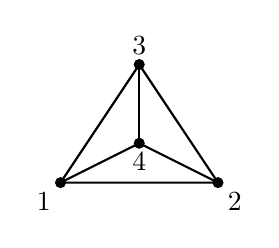
\begin{tikzpicture}
    % Define vertices (nodes)
    \fill (0,0) circle (2pt) node[below left] {1};
    \fill (2,0) circle (2pt) node[below right] {2};
    \fill (1,1.5) circle (2pt) node[above] {3};
    \fill (1,0.5) circle (2pt) node[below] {4}; % Center node for better look

    % Draw edges (connect every node to every other node)
    % \draw (0,0) -- (2,0) -- (1,1.5) -- (0,0) -- (1,0.5) -- (2,0) -- (1.5,1.5) -- (1,0.5) -- (0,0); % Not great, let's refine
    \draw[thick] (0,0) -- (2,0) -- (1,1.5) -- (0,0); % Outer triangle
    \draw[thick] (1,0.5) -- (0,0); % Diagonals
    \draw[thick] (1,0.5) -- (2,0);
    \draw[thick] (1,0.5) -- (1,1.5);
\end{tikzpicture}
\end{equation*}
ha bisogno di \(4\) colori. In generale, \(K_{n}\) è \(n\)-colorabile.
\end{esempio}

Nella tesi PhD di David Bayer:
\begin{quote}
una colorazione di un grafo è un punto di \(\A^{n}\) che annulla dei polinomi che ``contengono'' le informazioni sulle adiacenze nel grafo.
\end{quote}

Se \(G\) ha \(V(G) = \set{1,\dots,n}\), lavoro in \(\C[X_{1},\dots,X_{n}]\). Una colorazione è un insieme \(\V(I)\) con \(I\) ideale opportuno,
\(\V(I) \subseteq \C^{n}\).

Per studiare una \(k\)-colorazione, inserisco nell'ideale \(I_{k}\) delle condizioni i polinomi:
\begin{equation*}
X_{i}^{k}-1:\IMPLICA \V(X^{k}_{i}-1)\text{ radice \(k\)-esima dell'unità}.
\end{equation*}
Ogni radice \(k\)-esima dell'unità corrisponde ad un colore.

Supponiamo ad esempio che \(\set{1,2} \in E\). Considero quindi
\begin{align*}
X_{1}^{k}-1 &\in I_{k}\\
X_{2}^{k}-1 &\in I_{k}
\end{align*}
e quindi \(X_{1}^{k}-X_{2}^{k} \in I_{k}\). Quindi ogni colorazione \(p\) annulla \(X^{k}_{1}-X_{2}^{k}\):
\begin{equation*}
X_{1}^{k}-X_{2}^{k} = (X_{1}-X_{2}) \parentesi{g_{12}}{( X_{1}^{k-1} + X_{1}^{k-2}X_{2} +\dots + X_{2}^{k-1})}
\end{equation*}
Quindi, la condizione affinché due vertici adiacenti \uline{non} abbiano lo stesso colore, è che il polinomio di cui sopra non sia nullo.

Pongo quindi \(g_{12} \in I_{k}\). Questo è sufficiente per ottenere la condizione di cui sopra:
\begin{itemize}
\item se \(X_{1} = X_{2} = \xi\) radice \(k\)-esima dell'unità, allora
\begin{equation*}
g_{12}(\xi,xi) \neq 0
\end{equation*}
\item se \(X_{1}=\xi_{1}\neq\xi_{2} = X_{2}\) allora
\begin{equation*}
  g_{12}(\xi_{1},xi_{2}) = 0
\end{equation*}
\end{itemize}

Sostanzialmente, quindi, per ogni \(\set{i,j} \in E\), metto
\begin{equation*}
\frac{X_{i}^{k}-X_{j}^{k}}{X_{i}-X_{j}} \in I_{k}
\end{equation*}
L'ideale \(I_{k}\), quindi, è generato da
\begin{equation*}
\set{X_{i}^{k}-1}_{i=1,\dots,n}%
\cup%
\set{\frac{X_{i}^{k}-X_{j}^{k}}{X_{i}-X_{j}}}_{\set{i,j} \in E}
\end{equation*}
Si ha che le seguenti affermazioni sono equivalenti:
\begin{enumerate}
\item \(G\) è \(k\)-colorabile;
\item \(\V(I_{k}) \neq \emptyset\);
\item \(I_{k} \neq \K[X_{1},\dots,X_{n}]\)
\end{enumerate}
dove \(2.\Leftrightarrow 3.\) segue dal Nullstellensatz.

Quindi, l'algoritmo è, dato un grafo \(G\):
\begin{itemize}
\item costruisco \(I_{k}\);
\item calcolo la GB di \(I_{k}\);
\begin{itemize}
\item se GB di \(I_{k}\) è \(\set{1}\), allora \(G\) \uline{non è} \(k\)-colorabile;
\item se GB di \(I_{k}\) è \(\neq\set{1}\), allora \(G\) \uline{è} \(k\)-colorabile.
\end{itemize}
\end{itemize}
\newpage
\end{document}
